\chapter{Results}
\label{chapter:Results}

\section{Preprocessing}

\subsection{Integration of common datasets}

As mentioned in Section \ref{integration-method}, the gathered datasets were integrated into one depending on the diagnosis and tissue of origin, which are called integrated datasets (see Table \ref{tab:integrated-sets}). The distributions of the integrated datasets were normalized by quantiles in order to perform further analyses; an example is given in Fig. \ref{fig:norm}, the complete set of graphs are presented in Appendix \ref{dist-quantiles}. As it can be seen, the distributions of the samples had different shapes before normalizing; after quantile normalization is applied, the samples get a similar distribution, however the genes with low intensities, on the left tail, are not completely normalized. Additionally, these datasets required to be processed by \verb|ComBat| function since they came from different experiments. The PCA plots shown in Fig. \ref{fig:batchcorrection}a, present a clear separation given by the batch, which in this case corresponds to the distinct experiments. Moreover, Fig. \ref{fig:batchcorrection}b depicts the result of applying \verb|ComBat| to these datasets: the experiment variation is now negligible and DGE analysis can be carried out. 

\begin{table}[ht]
\centering
\caption{Source and number of samples included in each of the integrated datasets.}
\label{tab:integrated-sets}
\begin{tabular}{llcc}
\hline
\multicolumn{1}{c}{\textbf{Integrated dataset}} & \multicolumn{1}{c}{\textbf{Databases}} & \textbf{Control} & \textbf{Case} \\ \hline
\multirow{4}{*}{Prefrontal cortex PD} & GSE68719                           & 44           & 29           \\
                                      & GSE135036                          & 12           & 24           \\
                                      & BMC                       & 22           & 27           \\ \cline{3-4} 
                                      & \multicolumn{1}{r}{\textit{Total}} & \textbf{78}  & \textbf{80}  \\
\multirow{3}{*}{Prefrontal cortex HD} & GSE64810                           & 49           & 20           \\
                                      & GSE129473                          & 5            & 11           \\ \cline{3-4} 
                                      & \multicolumn{1}{r}{\textit{Total}} & \textbf{54}  & \textbf{31}  \\
\multirow{3}{*}{Parietal AD}          & GSE144254                          & 0            & 42           \\
                                      & AIBS (PaCx)                        & 46           & 37           \\ \cline{3-4} 
                                      & \multicolumn{1}{r}{\textit{Total}} & \textbf{46}  & \textbf{79}  \\
\multirow{3}{*}{Blood HD}             & GSE51799                           & 33           & 91           \\
                                      & GSE61405                           & 8            & 11           \\ \cline{3-4} 
                                      & \multicolumn{1}{r}{\textit{Total}} & \textbf{41}  & \textbf{102} \\
\multirow{3}{*}{Temporal AD}          & GSE104704                          & 10           & 12           \\
                                      & AIBS (TCx)                         & 50           & 41           \\ \cline{3-4} 
                                      & \multicolumn{1}{r}{\textit{Total}} & \textbf{60}  & \textbf{53}  \\
\multirow{3}{*}{Hippocampus AD}       & GSE67333                           & 4            & 4            \\
                                      & AIBS (HIP)                         & 50           & 36           \\ \cline{3-4} 
                                      & \multicolumn{1}{r}{\textit{Total}} & \textbf{54}  & \textbf{40}  \\
\multirow{3}{*}{Frontal AD}           & GSE125050                          & 57           & 36           \\
                                      & AIBS (FWM)                         & 47           & 38           \\ \cline{3-4} 
                                      & \multicolumn{1}{r}{\textit{Total}} & \textbf{104} & \textbf{74}  \\ \hline
\end{tabular}

\footnotesize FWM: Frontal white matter; HIP: Hippocampus; PaCx: Parietal cortex; TCx: Temporal cortex.
\end{table}

\begin{figure}%
    \centering
    \subfloat[\centering Before quantile normalization ]{{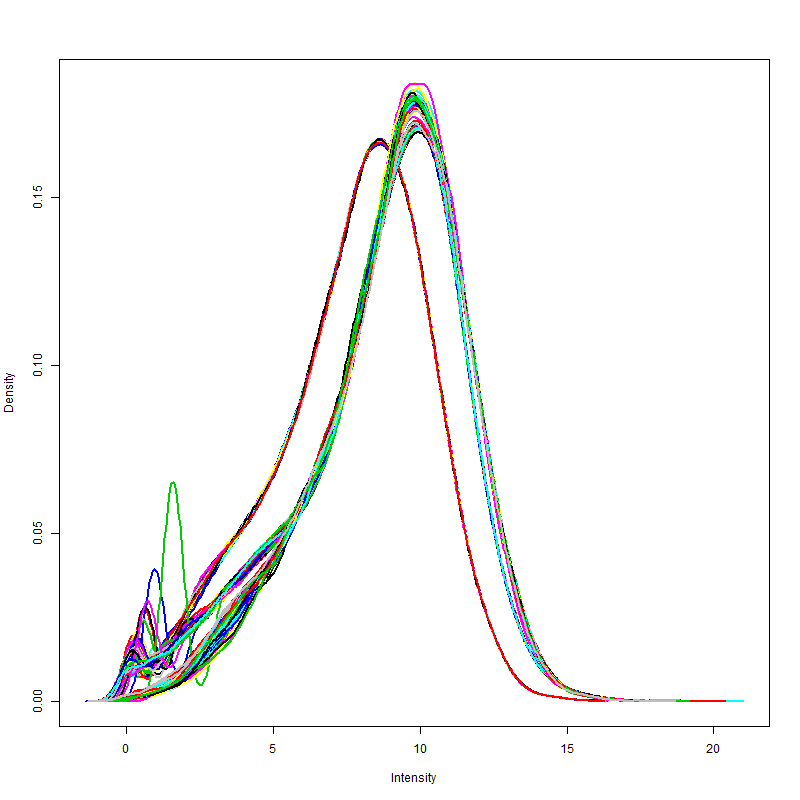
\includegraphics[width=5cm]{Figures/PD-densities_before.png} }}%
    \qquad
    \subfloat[\centering After quantile normalization ]{{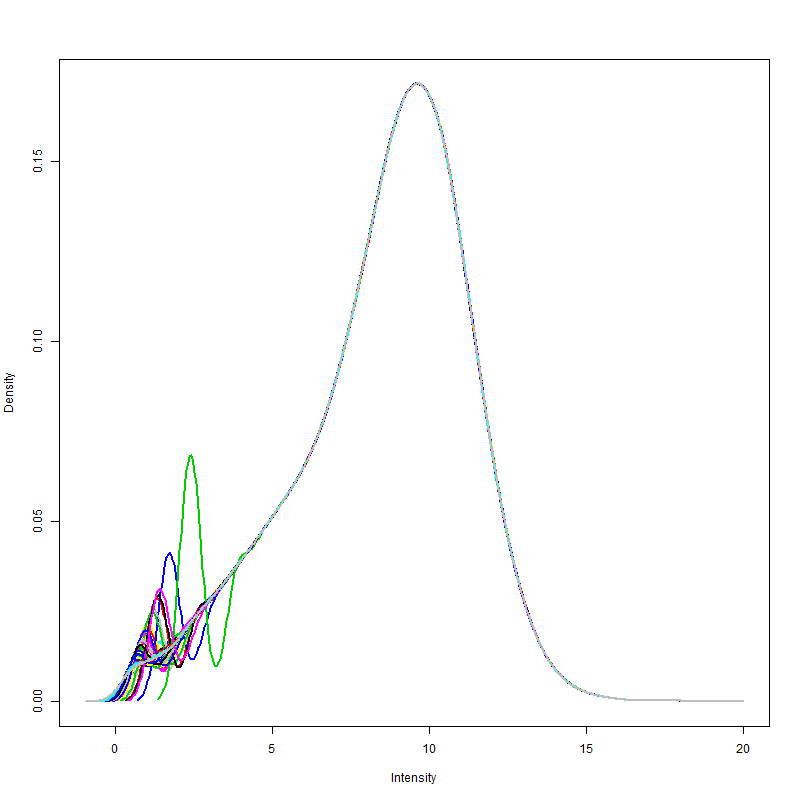
\includegraphics[width=5cm]{Figures/PD-densities_after.png} }}%
    \caption{Quantile normalization example for PCx-PD integrated dataset}%
    \label{fig:norm}%
\end{figure}

\begin{figure}%
    \centering
    \subfloat[\centering Before batch correction ]{{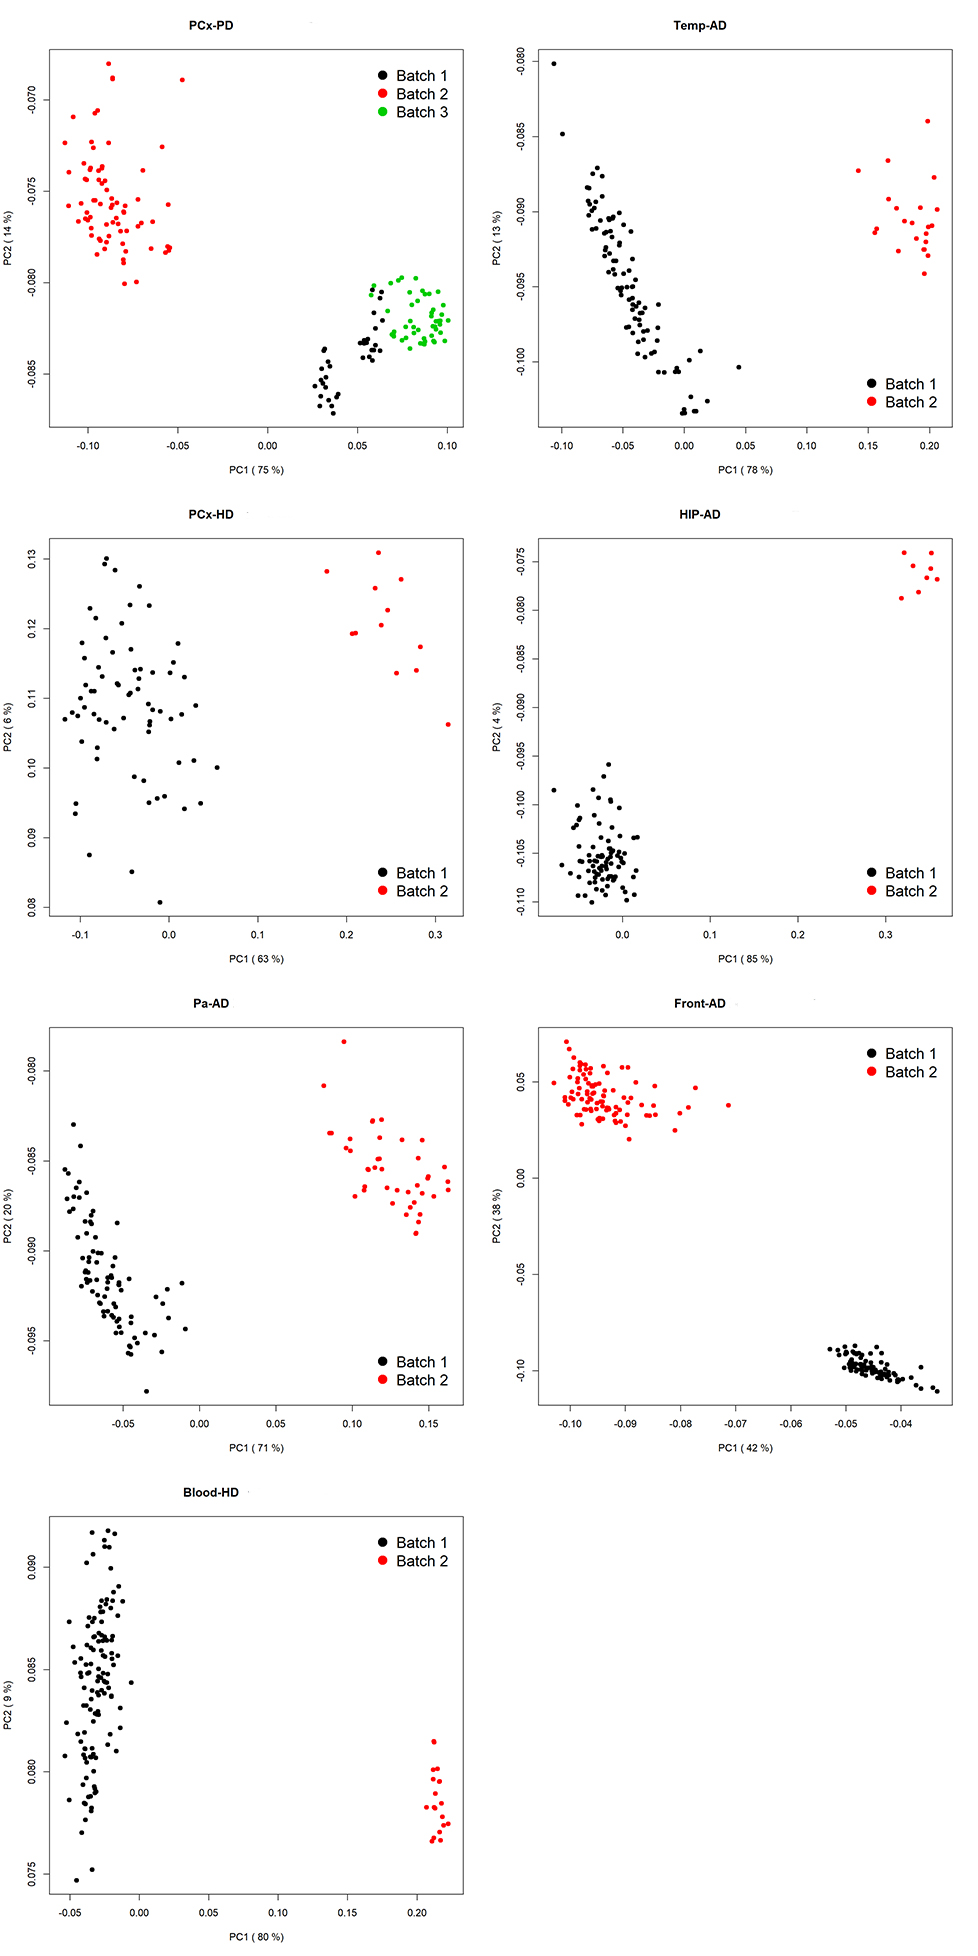
\includegraphics[width=6.5cm]{Figures/batchcorrectionA.jpg} }}%
    \qquad
    \subfloat[\centering After batch correction ]{{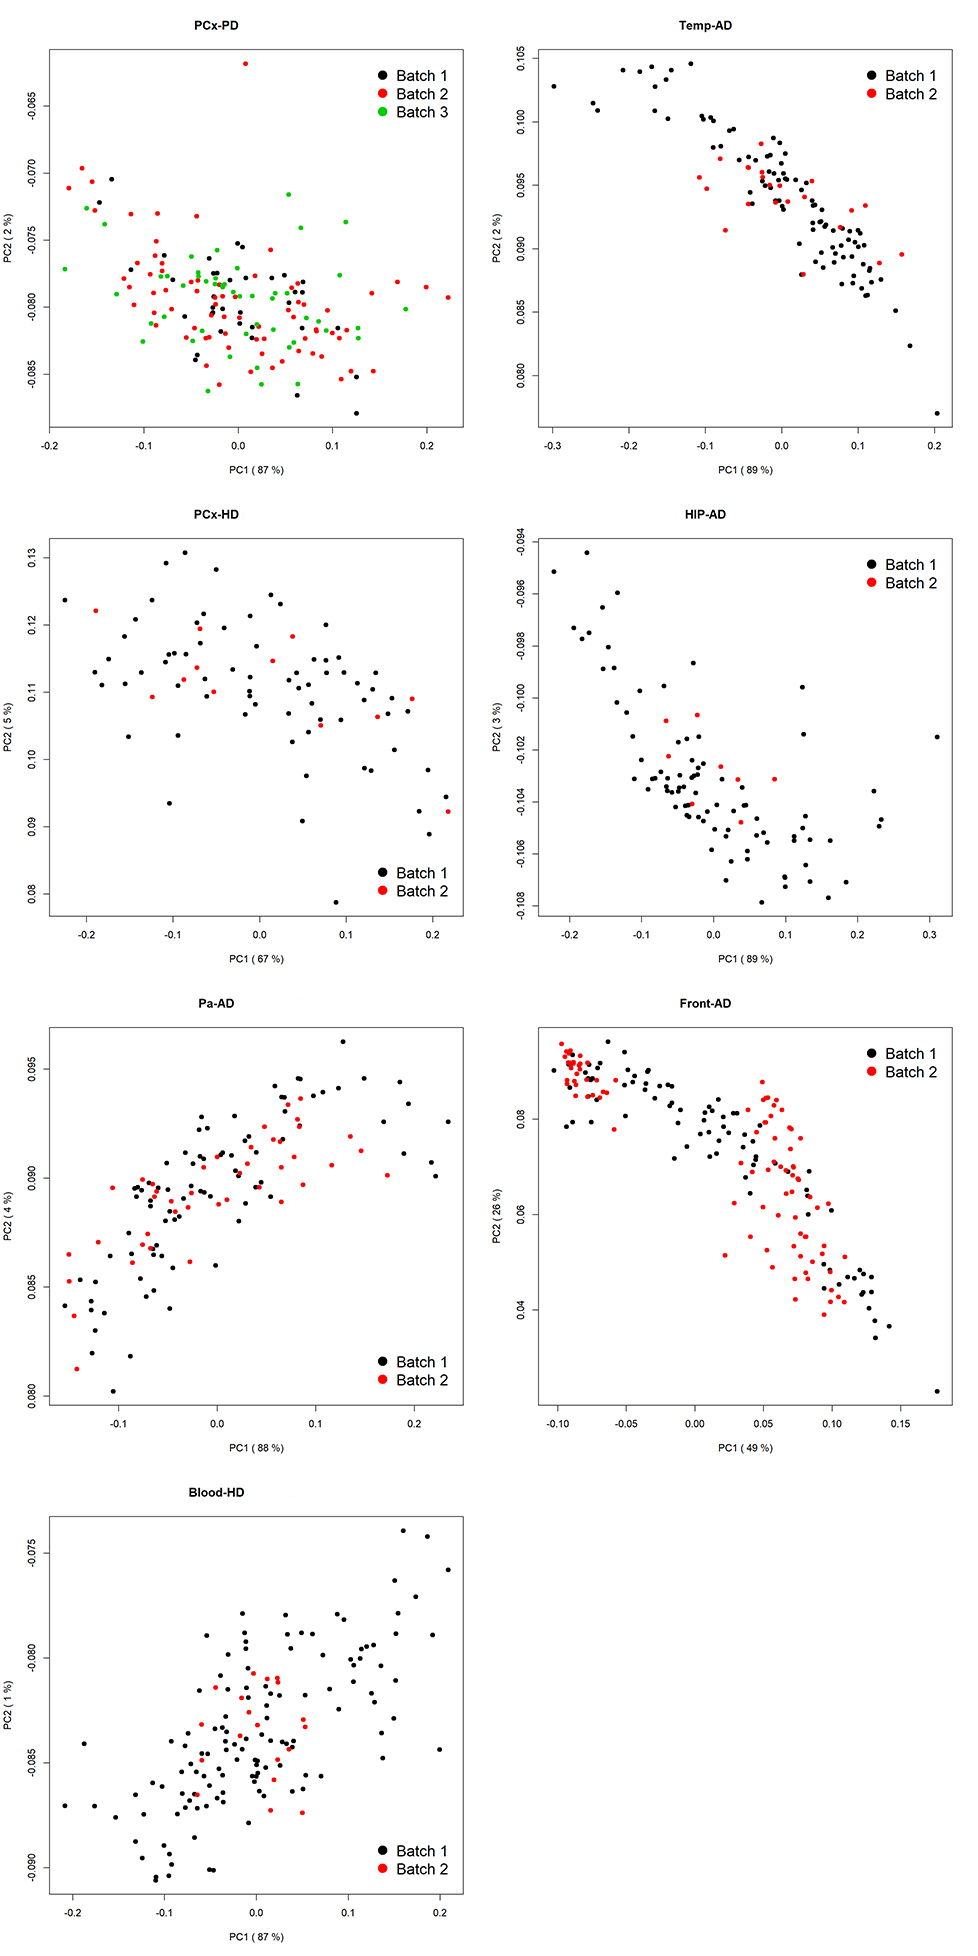
\includegraphics[width=6.5cm]{Figures/batchcorrectionB.jpg} }}%
\caption{PCA plots for each integrated dataset before and after batch correction with \texttt{ComBat} function.}
\label{fig:batchcorrection}%
\end{figure}

\subsection{Covariate identification}

Before continuing to the analytic phase, other preprocessing steps were done. The method explained in Section \ref{cov-method} identified the sex covariate as an important factor on the gene expression of all the sets. In addition, Braak score and age variables were only relevant in Fus-AD database (adjusted in DGE analysis); age had a slightly effect on the remaining sets (see Table \ref{tab:limma-cov}). Subsequently, the datasets were divided by the sex covariate, meaning that from one dataset it resulted in two datasets (female and male). Nevertheless, Prefrontal cortex PD (PCx-PD) and Prefrontal cortex HD (PCx-HD) integrated datasets were not partitioned by sex since the former consisted of approximate 85\% male samples, and the latter had no clinical information. The number of samples included in the split datasets are presented in the first three columns of Table \ref{tab:homosex-sets}.

As note, the most imbalance datasets before splitting by sex were Temporal AD (Temp-AD) and Frontal AD (Front-AD) with a ratio female/male of 39/74 and 68/110 on total samples, respectively. On the other hand, the smallest disproportion on control/case ratio was obtained by PCx-PD (78/80), Temp-AD-f (20/19), Hippocampus AD female split (Hip-AD-f) (22/21) and Front-AD-f (35/33); the remaining sets have an imbalance of at least 14 samples. This gives more evidence of the importance of partitioning the data by the sex covariate. 

\begin{table}[!ht]
\centering
\caption{Number of affected genes by the covariates according to the linear model generated with \textit{limma} for each dataset.}
\label{tab:limma-cov}
\begin{tabular}{llc}
\hline
\multicolumn{1}{c}{\textbf{Integrted Dataset}} & \multicolumn{1}{c}{\textbf{Covariates}} & \textbf{Affected number of genes} \\ \hline
PCx-PD   & Age   & 296   \\
         & Sex   & 15037 \\
         & PMI   & 1     \\
PCx-HD  & No information & \\
Blood-HD & Age   & 60    \\
         & Sex   & 12181 \\
Pa-AD    & Age   & 0     \\
         & Braak & 0     \\
         & Sex   & 14609 \\
Temp-AD  & Age   & 8     \\
         & Braak & 0     \\
         & Sex   & 18469 \\
Hip-AD   & Age   & 0     \\
         & Braak & 0     \\
         & Sex   & 12601 \\
Front-AD & Age   & 0     \\
         & Braak & 0     \\
         & Sex   & 15185 \\
Fus-AD   & Age   & 479   \\
         & Braak & 3255  \\
         & Sex   & 16168 \\ \hline
\end{tabular}

\footnotesize PMI: Post-mortem interval.
\end{table}

\begin{table}[!ht]
\centering
\small
\caption{Size of the integrated and Fus-AD datasets after sex partition and selection of core samples.}
\label{tab:homosex-sets}
\begin{tabularx}{1.0\textwidth}{L{1.8cm}C{1.8cm}C{1.8cm}C{1.8cm}C{1.8cm}C{1.8cm}C{1.8cm}}
\toprule
Dataset & All samples & All control & All case & Core samples & Core control & Core case \\
  \midrule
\textbf{PCx-PD}     & 158 & 78 & 80  & 106 & 50 & \textbf{56} \\
PCx-HD     & 81  & 52 & 29  & 54  & 32 & 22 \\
\textbf{Blood-HD-f} & 77  & 24 & 53  & 44  & 11 & \textbf{33} \\
\textbf{Blood-HD-m} & 66  & 17 & 49  & 39  & 6  & \textbf{33} \\
Pa-AD-f    & 56  & 18 & 38  & 37  & 14 & 23 \\
Pa-AD-m    & 69  & 28 & 41  & 44  & 22 & 22 \\
Temp-AD-f  & 39  & 20 & 19  & 23  & 11 & 12 \\
Temp-AD-m  & 74  & 40 & 34  & 47  & 28 & 19 \\
Hip-AD-f   & 43  & 22 & 21  & 30  & 16 & 14 \\
Hip-AD-m   & 51  & 32 & 19  & 34  & 24 & 10 \\
Front-AD-f & 68  & 35 & 33  & 36  & 18 & 18 \\
Front-AD-m & 110 & 69 & 41  & 69  & 49 & 20 \\
\textbf{Fus-AD-f}   & 130 & 33 & 97  & 91  & 26 & \textbf{65} \\
\textbf{Fus-AD-m}   & 159 & 37 & 122 & 114 & 29 & \textbf{85} \\
\bottomrule

\end{tabularx}
\end{table}


\subsection{Selection of core samples}

While examining the MAD PCA plots of all the new databases, it was observed that some control samples were placed in the case cluster, and vice-versa; this effect was considered as inter-heterogeneity among the sample groups. In view of this, NMF was employed as described in Section \ref{hete-method} to conclude with a more unvaried set of samples. In Fig. \ref{fig:outliers-plots}, the confusing samples are represented in green, these samples were removed from the 14 datasets in order to stay with purer groups. The last three columns of Table \ref{tab:homosex-sets} show the resulting sizes of the datasets after the selection of core samples for each group. The biggest loss occurred on Front-AD-f with a reduction of 47\% on total samples. On the other hand, the smaller decrease happen on Fus-AD-m with a loss of 28\% on all samples. A compelling aspect of this removal is that the majority of the datasets had a reduction of around 30\%. Moreover, the largest loss occurred on Blood-HD-m for control samples, and on Hip-AD-m for case samples with a 65\% and 47\% reduction, respectively. All the same, the lesser decrease happened on Fus-AD-f for control samples, and PCx-HD for case samples with a 21\% and 24\% loss. In consequence, 413 samples were removed out of 1181 ($\sim$35\%) from all the datasets in order to have more uniform sets.

\begin{figure}[ht]
    \centerline{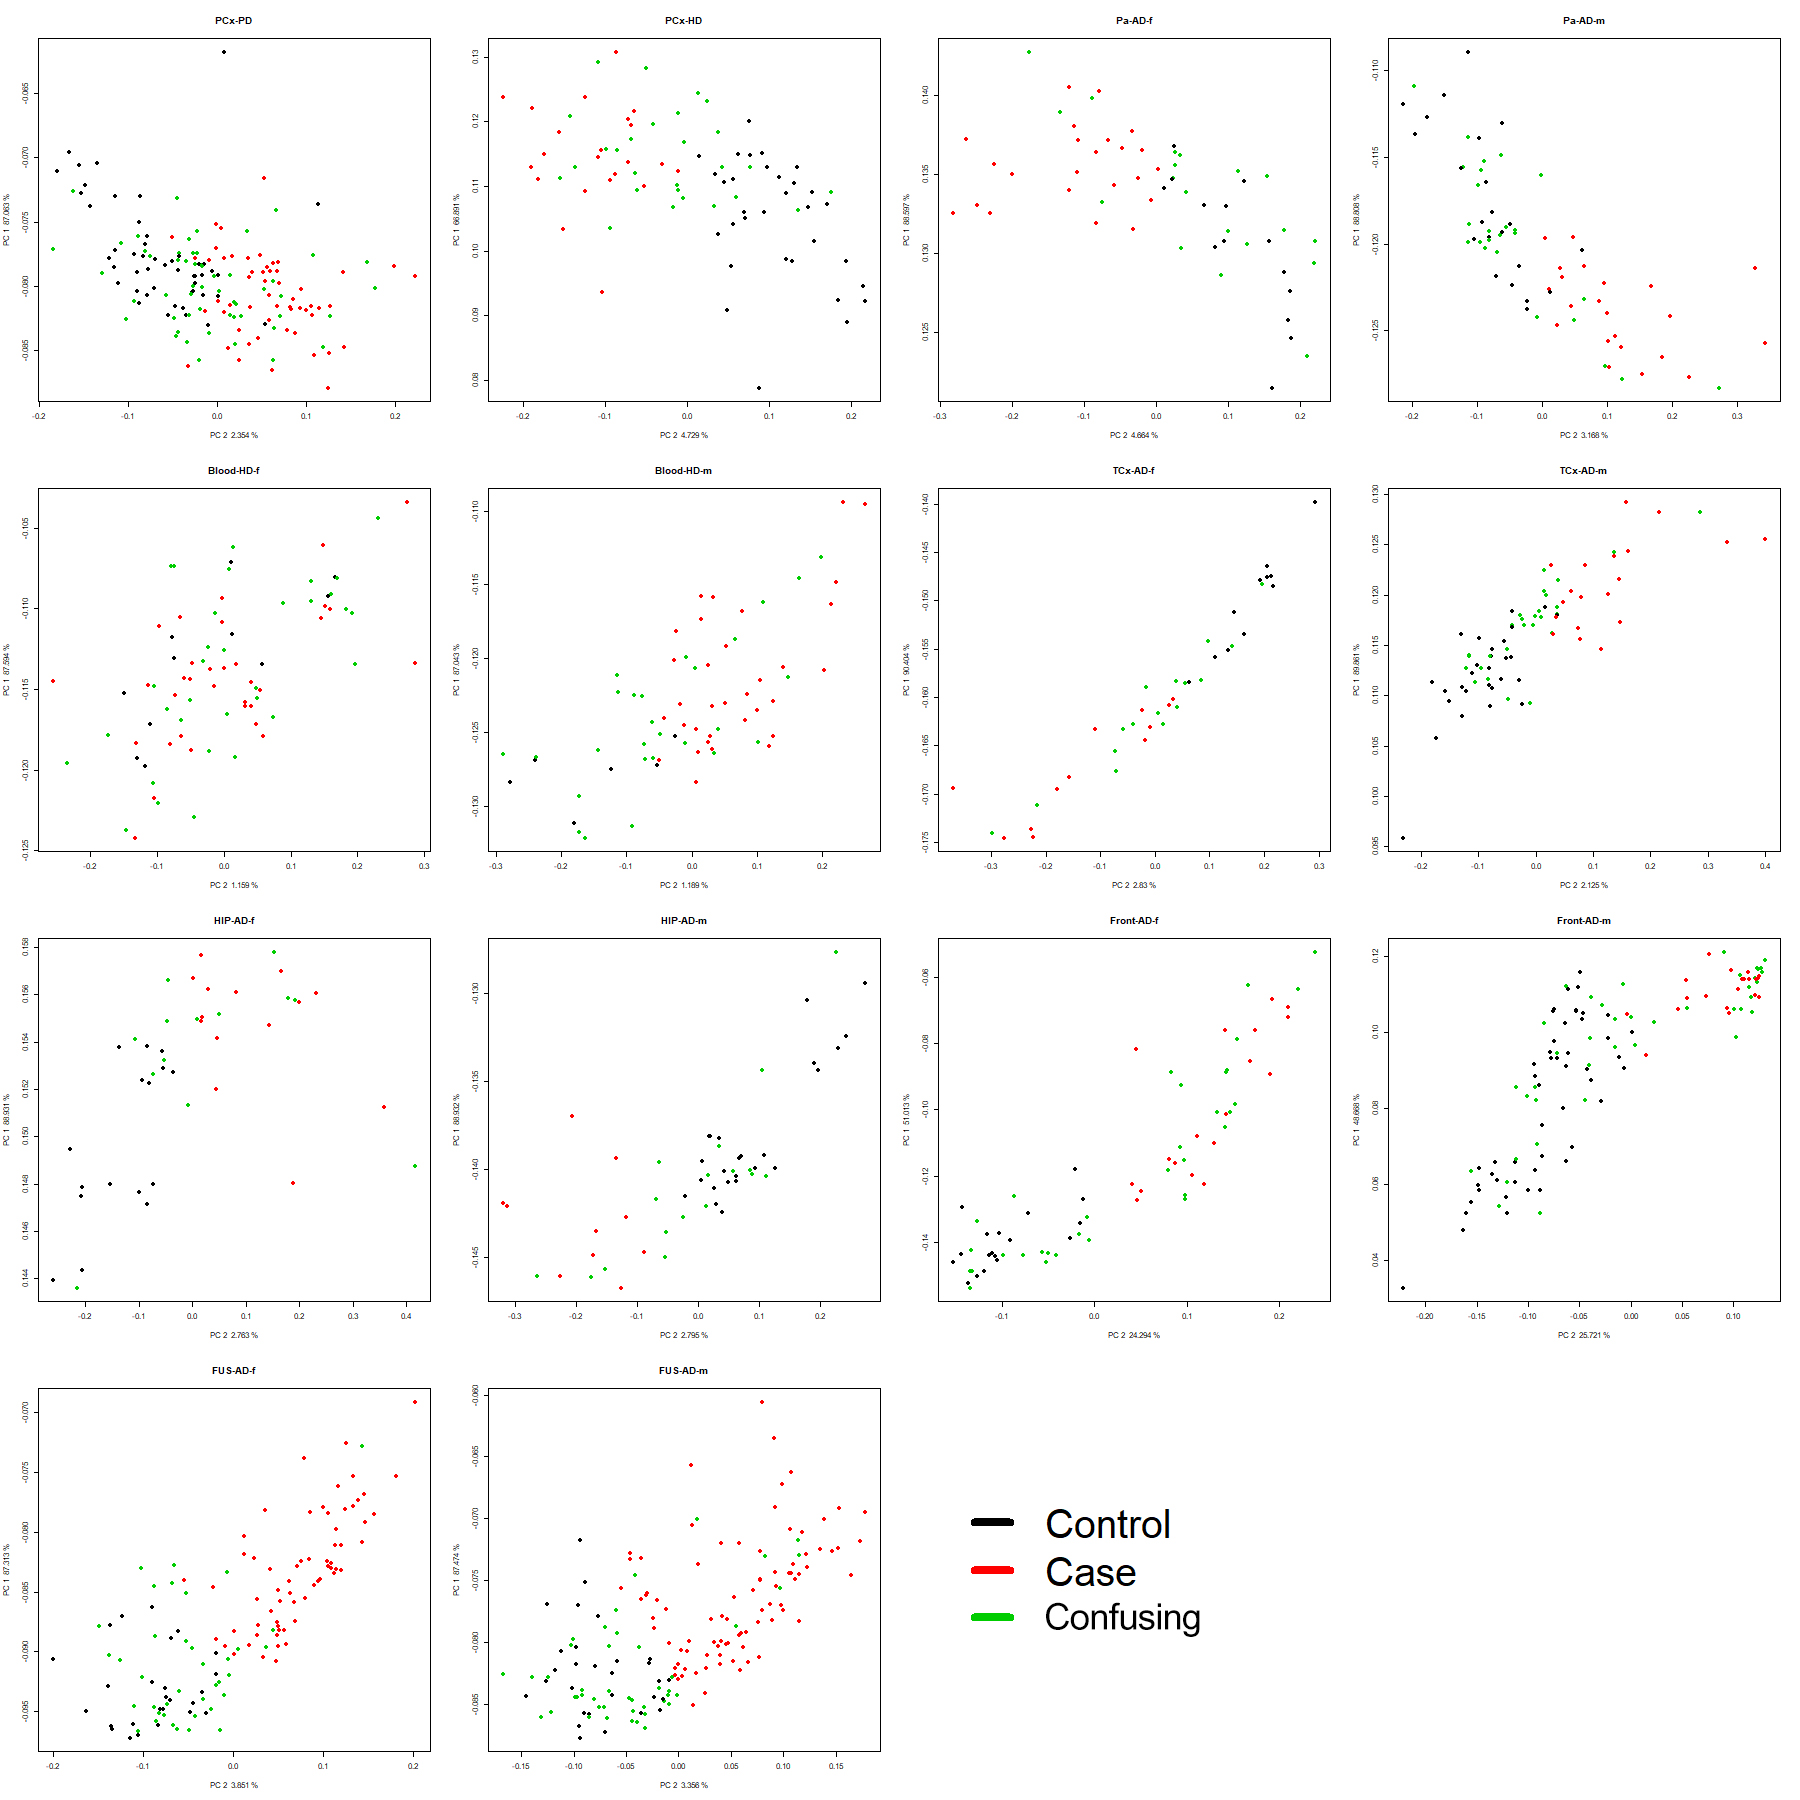
\includegraphics[width = 15cm]{Figures/outliers-removal.jpg}}
\caption{Selection of core samples represented by PCA plots.}
\label{fig:outliers-plots}
\end{figure}

\section{Molecular Subtype Identification}

The first step of the analytic phase, was the molecular subtype identification. As explained in the previous section (Section \ref{subtype-method}), NMF method was once again used to accomplish this step. Is important to mention that not all databases were eligible for this process, only PCx-PD, Blood-HD and Fus-AD were analyzed here, since they had more than 30 case samples (datasets which names are in bold in Table \ref{tab:homosex-sets}). After obtaining the membership of each sample by NMF, the expression data of these five sets were processed by PCA and their results were plotted and coloured according this membership; the graphs are presented in Fig. \ref{fig:pca-subtype}. Interestingly, three molecular subtypes were determined in female splits and PCx-PD, while in male splits only two subtypes were ascertained. On further analyses, the differences between subtypes will be assessed.

\begin{figure}[ht]
    \centerline{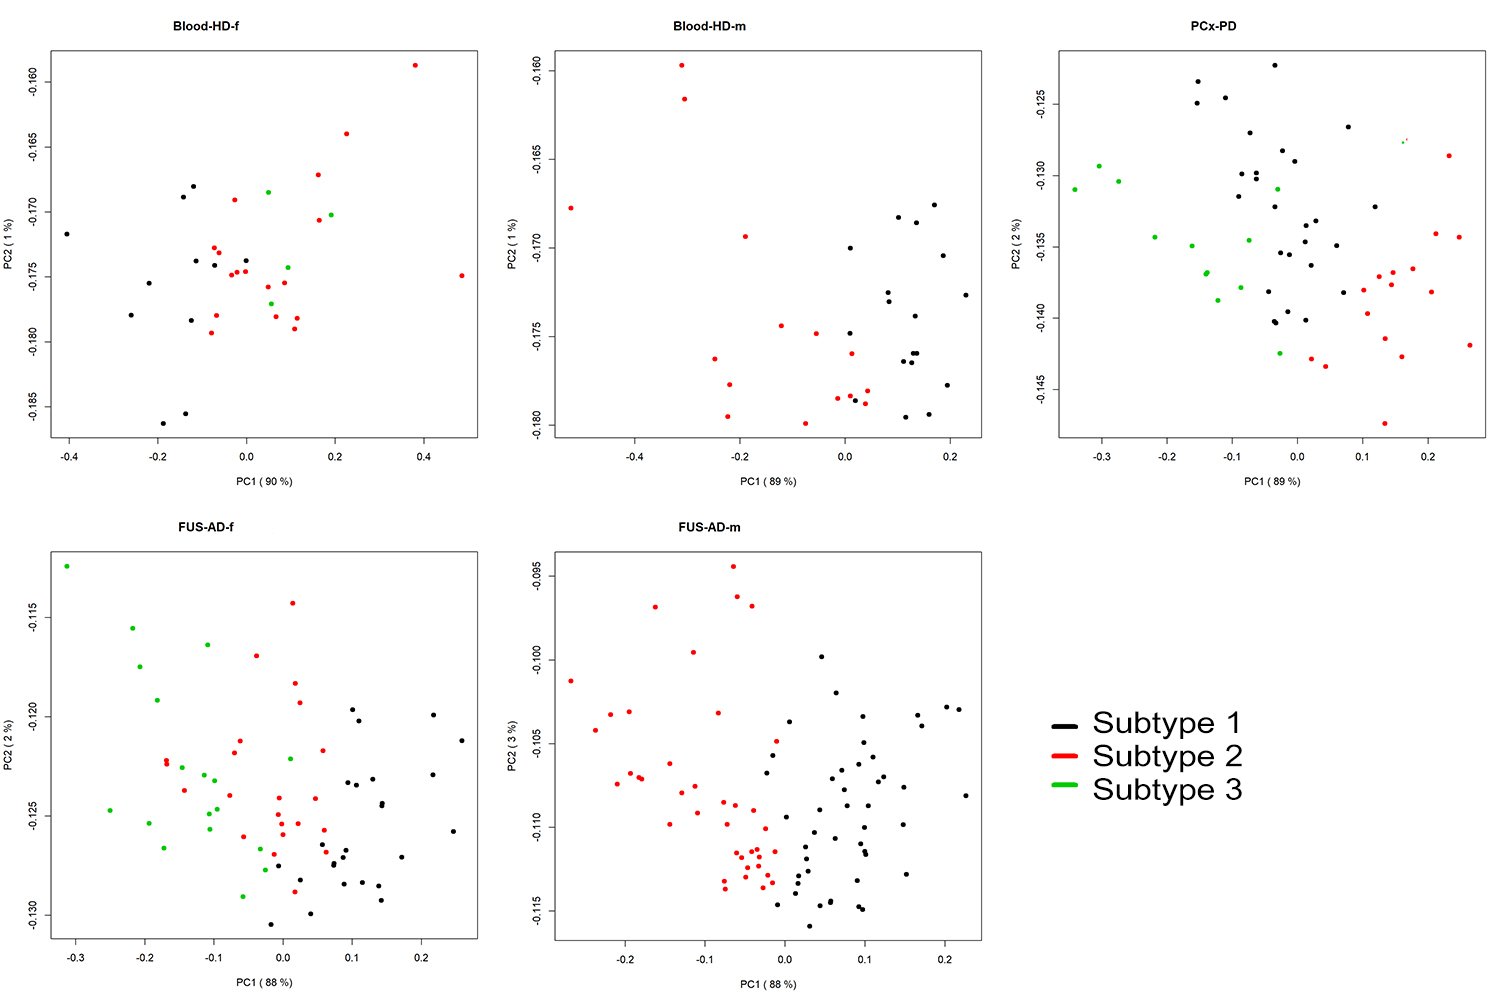
\includegraphics[width = 13cm]{Figures/pca-subtype.jpg}}
\caption{Molecular subtype identification presented by PCA plots.}
\label{fig:pca-subtype}
\end{figure}

\section{Cell Proportion Estimation} \label{result-cells}

Before reaching to the DGE analysis, the cell proportion estimation was performed on the core samples of each datasets. As mentioned in Section \ref{cells-method}, the estimation of immune cell type proportion was done separately from the brain cell type proportion prediction, and using different algorithms. Therefore, this section is divided into two steps which are described below.

\subsection{Immune cell types}

The estimation of abundances of immune cell types from a mixture cell population was done by CIBERSORTx, as explained in Section \ref{immune-method}. The analysis is simple in the way that the web service carries with all the work, the important part is to upload the required matrices in the correct form. After imputing the corresponding data and parameters, the job takes a few minutes to finish and the results can be gathered. Subsequently, $t$-tests were applied to these results in order to distinguish significant change in the immune cells population between control and case samples; Fig. \ref{fig:cibersort} presents these changes.

\begin{figure}[ht]
    \centerline{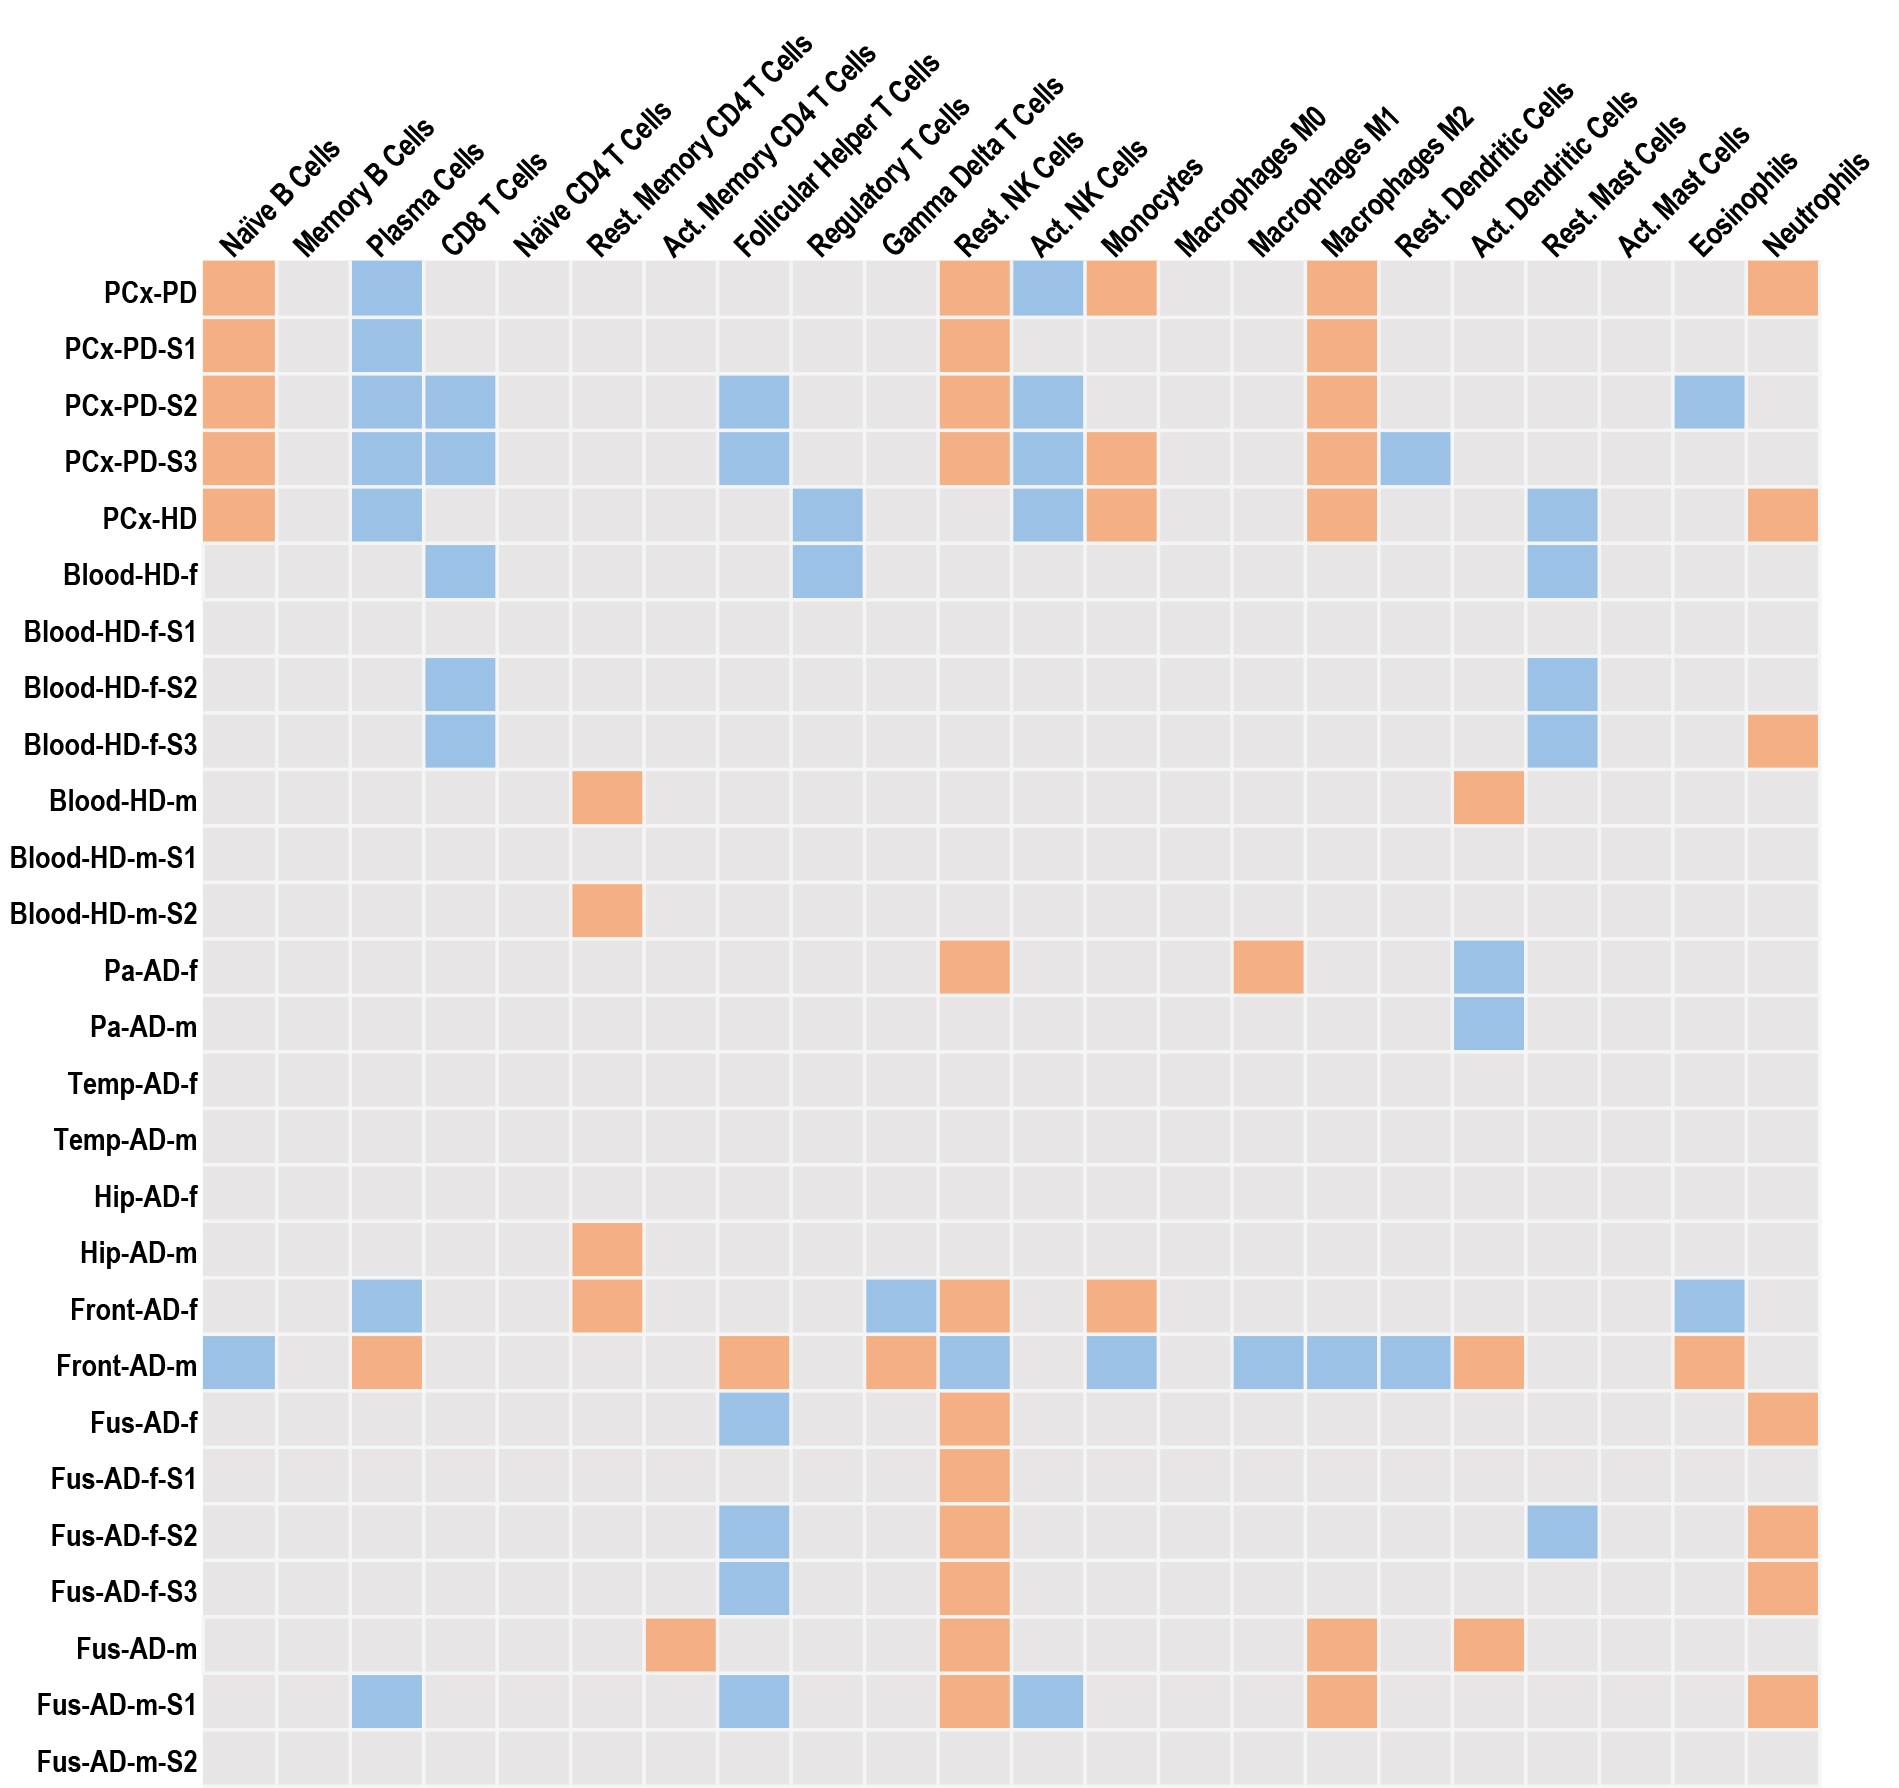
\includegraphics[width = 13cm]{Figures/immune.jpg}}
\caption{Heatmap representation for calculated changes of 22 immune cell types abundances between control and case samples.}
\footnotesize Orange: Case $>$ Control; blue: Control $>$ Case; gray: not significant change (q-value $>$ 0.05).
\label{fig:cibersort}
\end{figure}

\textbf{PCx-PD.} The first row of Fig. \ref{fig:cibersort} shows the results obtained in the comparison between control and PD samples. These suggest that the immune system is depressed since the naïve B cells are more abundant in the case samples than in control samples. In addition, there are more plasma cells in control; this behavior is expected since naïve B cells transform to plasma cells or memory B cells. Also, the immune system could be depressed in PD because the population of resting NK cells increased, while in control there are more activated NK cells. Lastly, markers of inflammation are higher in PD than in control: monocytes, macrophages M2, and neutrophils.

Moving forward to PD subtypes, the molecular subtype 1 of PD in prefrontal cortex (PCx-PD-S1) appears to have fewer alterations than the whole PD samples. PCx-PD-S1 could also have immune system depression as PD due to the increase in naïve B cells and resting NK cells, and reduction in plasma cells. Moreover, high macrophage M2 population suggests that a possible inflammation is trying to be constrained. PCx-PD-S2 is similar to PCx-PD-S1 except the former have four more changes, then the interpretation for S1 applies to S2. In addition, there are more plasma cells in control as well as follicular helper T Cells; naïve B cells transform to plasma cells or memory cells aided by the follicular helper T cells. If there are less follicular helper T cells in case samples, then it could mean that there will be less plasma cells and more naïve B cells. Normally, low eosinophil abundance is not of concern, but it could mean there is an increase in cortisol. Finally, PCx-PD-S3 has the largest amount of variations between case and control, many similar to PD. Same as for the other subtypes, the results suggest a depressed immune system, and a process for constraining inflammation. Moreover, PCx-PD-S3 has lower monocyte and resting dendritic cells abundance in case than in control which also suggest an immunodeficiency; dendritic cells are involved in antigen-presentation.

\textbf{PCx-HD.} The results obtained from this analysis suggest that the decrease in HD of regulatory T cells may lead to proliferation of T cells. Similar to PD, the immune system could be depressed since the population of naïve B cells is high and the abundance of plasma cells is low in HD, as well as the activated NK cells. Morevoer, monocytes, neutrophils and macrophages M2 are high in HD suggesting the presence of an inflammation process. Finally, there are more resting dendritic cells in control than in HD.

\textbf{Blood-HD-f.} As it can be seen in the figure, the results from Blood-HD-f have similar changes to PCx-HD, which adds up to theory since immune cells travel by blood. The decrease of regulatory T cells in HD may lead to proliferation of T cells, as mentioned above; however, dataset has also a reduction in the population of CD8 T cells in HD. Likewise, there is a decrement in the abundance of resting mast cells. Analyzing the molecular subtypes, Blood-HD-f-S1 has none significant change. Blood-HD-f-S2 has two similar changes with Blood-HD-f: a decrease in CD8 T cells and resting mast cells in case. Lastly, Blood-HD-S3 has also the same variation on CD8 T cells and resting mast cells, but includes an increase in neutrophiles in HD (suggesting inflammation) which is similar to PCx-HD. All these variations suggests a compromised immune system, specially because CD8 T cells and resting mast cells are low in case condition.

\textbf{Blood-HD-m.} It would be expected that Blood-HD-m was alike to PCx-HD as well, but it was not the situation. Maybe the PCx-HD dataset contained more female samples, however it cannot be known since the database had no additional clinical information. Moving on, Blood-HD-m has an increase in resting memory CD4 T cells. The latter suggests that the antigen has not been present yet. Additionally, HD has higher activated dendritic cells than control samples, which may mean that the antigen-presentation is happening. 
Continuing with the molecular subtype explanation, Blood-HD-m-S1 does not have any significant changes in the population of immune cells between control and HD samples. On the other hand, Blood-HD-m-S2 has just one change: increased abundance of resting memory CD4 T cells in HD, which also happens in Blood-HD-m.

\textbf{Pa-AD-f.} The variations in Pa-AD-f are few and prompt to a response of inflammation: high abundance of macrophage M1 in case. In AD, the increase in resting NK cells and the reduction in activated dentritic cells could suggest a depressed antigen-presentation.

\textbf{Pa-AD-m.} This dataset only contain one alteration which is common to Pa-AD-f, the loss of activated dendritic cells in AD.

\textbf{Temp-AD-f.} No significant changes in the abundance of immune cell types.

\textbf{Temp-AD-m.} No significant changes in the abundance of immune cell types.

\textbf{Hip-AD-f.} No significant changes in the abundance of immune cell types.

\textbf{Hip-AD-m.} This set resulted in only one alteration. The analysis implies an increment in resting memory CD4 T cells in AD which is not present in the female counterpart. Interestingly, it is the same result obtained for Blood-HD-m-S2.

\textbf{Front-AD-f.} Many of the changes occurring in Front-AD-f may imply a depression in the immune system processes: decrease in plasma cells and gamma delta T cells, and increase in resting memory CD4 cells and resting NK cells in AD. Moreover, a high monocyte abundance could mean inflammation. Low eosinophils could imply production of cortisol.

\textbf{Front-AD-m.} The rise of plasma cells, activated NK cells, follicular helper T cells, activated dendritic cells and gamma delta T cells suggest an active immune system. On the other hand, a contradiction may occurre since macrophages M1 and M2, and monocytes are decreased, and eosinophils are increased in AD. The latter tells there is inflammation along with an active immune response, the former suggests no inflammation process. Furthermore, both sexes have the same change, but the orientation is given in opposite direction.

\textbf{Fus-AD-f.} Similar to other results, the changes imply an inflammation response and depressed immune system in AD. The latter is given by the low presence of follicular helper T cells, and high abundance of resting NK cells. The former is suggest by the high concentration of neutrophils. 

Moving on to molecular subtype explanation. Interestingly, the three subtypes have an increase in resting NK cells in case; S2 and S3 have a decrease in follicular helper T cells as well as an increase in neutrophils, which may represent an inflammation process. What is more, Fus-AD-f-S2 uniquely has a reduction of active mast cells in AD.

\textbf{Fus-AD-m.} Fus-AD-f and Fus-AD-m have one resemblant variation in activate NK cells. Likewise, high abundance of macrohpage M2 may signify an inflammation response. Moreover, when there are activated dendritic cells, the antigen-presentation process has been initialized. The aforementioned makes sense with the high activated memory CD4 T cells abundance in AD.

The interpretation of the molecular subtypes suggests that, similar to the female counterpart, male subtype 1 presents an increase of resting NK cells and loss of follicular Helper T cells; however, Fus-AD-m-S1 contains a decrease in plasma cells in the case condition as well as in active NK cells. Moreover, this subtype implies a possible inflammation given by the rise of neutrophils and macrophages M2 in case; the latter is shared with Fus-AD-m. Finally, Fus-AD-m-S2 does not have any significant alterations among the immune cells.

\subsection{Brain cell types}

The prediction for brain cell type population was performed with \textit{BRETIGEA}; in Section \ref{brain-method} the process is described. Similar to the estimation of immune cell types abundance, the brain cell types were calculated first in order to make a comparison between the means of each group and evaluate if a possible difference is present. The results of the $t$-tests are depicted in Figure \ref{fig:bretigea}.

\begin{figure}[ht]
    \centerline{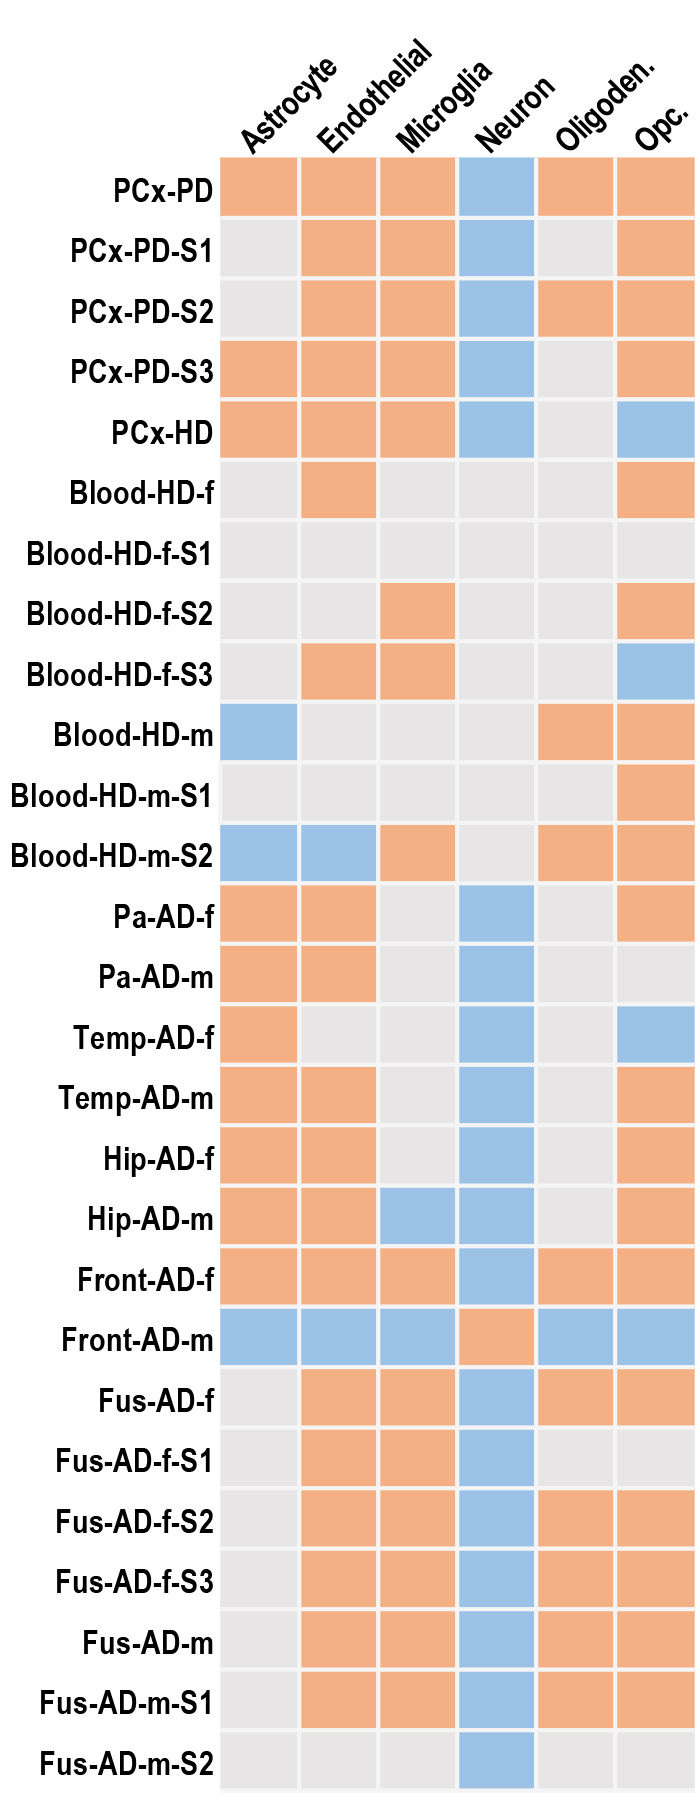
\includegraphics[width = 4cm]{Figures/brains.jpg}}
\caption{Heatmap representation of calculated changes of 6 brain cell types abundances between control and case samples.}
\footnotesize Orange: Case $>$ Control; blue: Control $>$ Case; gray: not significant change (q-value $>$ 0.05).
Opc: oligodendrocyte precursors.
\label{fig:bretigea}
\end{figure}

\textbf{PCx-PD.} The first row of Fig. \ref{fig:bretigea} depicts the changes occurred between control and PD samples. These results suggest that neurons decreases in the samples with PD, while all the other cells increase in this condition. Analyzing the molecular subtypes, it can be seen that PCx-PD-S1 has similar variations as PD: there is a loss of neurons in case samples, as well as an increment of endothelial cells, microglia and oligodendrocyte precursors (Opc). Same as before, PCx-PD-S2 has a reduction of neurons in case condition. Additionally, S2 has an increase of oligodendrocytes in case, which will be relevant in further studies. Finally, PCx-PD-S3 has a rise in all type of brain cells except for neuron (reduction) and oligodendrocytes (no significant change). In summary, PD and its three subtypes are concordant with the reduction of neurons and increment in the other cell types. According to \cite{bryois}, in PD samples, it has been identified a decrease of enteric, cholinergic and monoaminergic neurons in substantia nigra, an increase in oligodendrocytes, and no change in microglia.  

\textbf{PCx-HD.} Corresponding to \cite{bookHD}, HD samples have presented a decrease of neurons, an increase of microglia and astrocytes, and no significant change of oligodendrocytes. In this dataset, the results coincide with literature. However, there is no sufficient information on texts about the variations of endothelial cells and Opc; the results of this analysis imply an increase of the former an a decrease of the latter.

\textbf{Blood-HD-f.} As it can be observed from the Fig. \ref{fig:bretigea}, the pattern of PCx-HD is very different from the pattern of Blood-HD-f, just resembling on the increase of endothelial cells. It can be the situation that the results are not precise since they were obtained from blood samples. On the other hand, Blood-HD-f-S2 and S3 do have an increment of microglia in case samples. However, none of the three subtypes nor the main Blood-HD-f set conclude with a decrease in neural cells. S1 is dissimilar to S2 and S3 because it does not contain any significant change. S2 shares the alteration in Opc. with S3, but the change is given in the opposite direction.

\textbf{Blood-HD-m.} The male dataset of Blood-HD has one more variation than its female counterpart. Although, it does not include a change in neuron abundance and has a decrease of astrocytes, it has an increment of oligodendrocytes and Opc in HD. Moreover, the alterations in the molecular subtype 2 of Blood-HD-m are alike to the main set. The three datasets resulted in an increase of Opc. The differences are that Blood-HD-m-S1 just contains one change (Opc.), and S2 have reduced endothelial cells in case samples, and has rose microglia numbers. The only similarity between these datasets and PCx-HD is the increase of microglia in HD.

\textbf{Pa-AD-f.} According to \cite{ekonomou}, in AD, astrocyte and microglia abundance increase with the severity of the disease since neurons die and the cerebral tension must be maintained. However, no information was found about endothelial cells, oligodendrocytes and Opc., but reason suggests they also may increase in order to keep the cerebral tension stable. The results match the literature because astrocytes, endothelial cells and Opc. have an increment in AD. In addition, neurons are reduced. Nevertheless, microglia has no significant change in Pa-AD-f.

\textbf{Pa-AD-m.} This dataset is very similar to the female set. It has the same variations of astrocytes, endothelial cells and neurons, which agrees the texts as well. However, it does not involve an alteration in Opc.

\textbf{Temp-AD-f.} The most relevant alterations are the reduction of neuron and the increment of astrocytes in AD since they are mentioned in the text. However, it does not have a significant change in microglia and oligodendrocyte abundance. In addition, there appears to be a loss of Opc.

\textbf{Temp-AD-m.} Neurons and astrocytes seem to have the known change direction. Likewise, Temp-AD-m has increased endothelial cells and Opc, which might coincide with reason. On the other hand, Temp-AD-m and Temp-AD-f have just two similar variations.

\textbf{Hip-AD-f.} The reduction of neurons in AD goes along with variations found in literature, as well as the increment of astrocytes. Moreover, the set has an increase in endothelial cells and Opc. Interestingly, Pa-AD-f and Temp-AD-m share exactly same variations with Hip-AD-f.

\textbf{Hip-AD-m.} The resulted alterations between both sexes in this tissue are the same, except for the reduction of microglia which appears in the male set. Therefore, the interpretation for Hip-AD-f also pertain to this set apart from the loss of microglia in AD.

\textbf{Front-AD-f.} This database has all possible significant variations. What is more, all of these variations concur with those described in literature above; especially, rise of astrocyte numbers and decrement of neuron abundance.

\textbf{Front-AD-m.} An equivalent situation occurred in the estimation of immune cell type proportion with this tissue: the changes have exactly the inverse direction between sexes. Nevertheless, the results of the male set do not agree with the variations found in literature.

\textbf{Fus-AD-f.} The alterations estimated in this dataset are similar to those identified in Front-AD-f, except for astrocyte. Hence, its variations mostly coincide with literature. Moreover, Fus-AD-f-S2 and S3 have exactly the changes and directions; Fus-AD-f-S1 shares its variations with the other two subtypes, but does not include the increment in oligodendrocytes and Opc. The molecular subtypes are resemblant to AD.

\textbf{Fus-AD-m.} Interestingly, both sexes in fusiform gyrus obtained the same results in this analysis; then, the interpretation of Fus-AD-f also belongs to the male set. Furthermore, Fus-AD-m-S1 is equivalent to the whole AD set. Finally, Fus-AD-m-S2 only contains a reduction of neuron abundance.

It should be noted that all the databases, regardless of the disease or tissue the samples were originated, have a consistent pattern, with exception of blood sets and Front-AD-m. A clear blue line is appreciated in the neuron column. Additionally, a orange frame surrounds this line in Fig. \ref{fig:bretigea}.

\section{Differential Gene Expression Analysis} \label{res-dgea}

The DGE analysis is one of the key examinations in this study since its results are utilized in the following four steps. After all, in the preprocessing phase and the molecular subtype identification, the datasets are introduced to \textit{limma} as explained in Section \ref{limma-method}. The LFC threshold in absolute value was set to 1; the threshold for subtypes varied according to amount of DEGs found in each comparison. Table \ref{tab:de-genes} reports the number of DEGs identified, both up- and down-regulated, along with the LFC threshold defined for each dataset. What is more, the number of samples and the LFC threshold do not correlate with the number of DEGs found (Spearman correlation test with p-value equal to 0.57 and 0.91, respectively). Furthermore, the heatmap for each comparison can be found in Appendix \ref{de-heatmaps}. It is important to highlight that the reference of contrast in all comparisons are the case samples.

\begin{table}[!ht]
\centering
\caption{Number of differentially expressed genes (DEGs) per dataset.}
\label{tab:de-genes}
\begin{tabular}{lccc}
\hline
\multicolumn{1}{c}{\textbf{Dataset}} & \textbf{LFC threshold} & \textbf{Number of DEGs} & \textbf{Number of Samples} \\ \hline
PCx-PD        & 1    & 383  & 104 \\
PCx-PD-S1     & 1.6  & 13   & 27  \\
PCx-PD-S2     & 1.6  & 475  & 16  \\
PCx-PD-S3     & 1.6  & 217  & 12  \\
PCx-HD        & 1    & 1857 & 54  \\
Blood-HD-f    & 1    & 27   & 44  \\
Blood-HD-f-S1 & 1    & 1270 & 11  \\
Blood-HD-f-S2 & 1    & 186  & 18  \\
Blood-HD-f-S3 & 1    & 1287 & 4   \\
Blood-HD-m    & 1    & 277  & 39  \\
Blood-HD-m-S1 & 1.25 & 42   & 18  \\
Blood-HD-m-S2 & 1.25 & 62   & 15  \\
Pa-AD-f       & 1    & 195  & 37  \\
Pa-AD-m       & 1    & 89   & 44  \\
Temp-AD-f     & 1    & 239  & 23  \\
Temp-AD-m     & 1    & 105  & 47  \\
Hip-AD-f      & 1    & 23   & 30  \\
Hip-AD-m      & 1    & 100  & 34  \\
Front-AD-f    & 1    & 3832 & 36  \\
Front-AD-m    & 1    & 3560 & 69  \\
Fus-AD-f      & 1    & 2090 & 91  \\
Fus-AD-f-S1   & 1.5  & 1142 & 25  \\
Fus-AD-f-S2   & 1.5  & 3041 & 22  \\
Fus-AD-f-S3   & 1.5  & 2538 & 18  \\
Fus-AD-m      & 1    & 1265 & 114 \\
Fus-AD-m-S1   & 1.5  & 2580 & 46  \\
Fus-AD-m-S2   & 1.5  & 577  & 39   \\ \hline
\end{tabular}
\end{table}

\sloppy
\textbf{PCx-PD.} Beginning with the interpretation of PCx-PD results, it can be seen in heatmap (Appendix \ref{DE-pcx-pd}) a defined contrast between the up-regulated control section and down-regulated PD section. However, in the over-expressed block of case, there are some samples which have blue (down-regulated) segments. This event may involve possible molecular subtypes which explain the divergent behaviour.

\textbf{PCx-HD.} Appendix \ref{DE-pcx-hd} presents the heatmap for PCx-HD dataset. The resulting pattern contains a clear contrast of four blocks. It seems the variability within case is less than within control. Although, there are some samples out of pattern, a subtype analysis could not be performed because there were no sufficient HD samples. In general, the pattern shows consistency.

\textbf{Blood-HD.} Blood-HD-f set has no defined pattern in its heatmap (Appendix \ref{DE-blood-hd-f}), specially since only 27 DEGs were found. Interestingly, after subtype characterization, hundreds more were obtained as shown in Table \ref{tab:de-genes}. Likewise, the heatmap presented in Appendix \ref{DE-blood-hd-m} for the male set does not show contrast with the case samples. However, when it is divided by subtype, a somehow more apparent pattern is seen. Moreover, a comparison of identified DEGs between female and male was performed and zero genes were found in the intersection, for both up- and down-regulated DEGs (Appendix \ref{Venn-degs}).

\textbf{Pa-AD.} Moving to Pa-AD dataset, although the male part have just 89 DEGs, four blocks are clearly seen its heatmap (Appendix \ref{DE-pa-ad-m}). However, some samples, both case and control, have distinct expressions than the others. Specifically, the fourth control sample (left to right) which has almost all genes sub-expressed, as well as the fourth and twelfth case samples. For the female counterpart (Appendix \ref{DE-pa-ad-f}), control samples have almost no variation. On the other hand, the AD section contains anomalous samples, those that do not follow the general pattern. Furthermore, 32 over-expressed and 40 under-expressed DEGs were identified in both sexes, while 75 and 48 were unique up- and down-regulated DEGs for female set, respectively; 13 and 4 for the male set, respectively (see Appendix \ref{Venn-degs}). The above may imply that the pathogenesis of female and male patients are not so distinct between them.

\textbf{Temp-AD.} For Temp-AD-f dataset, in general, a clear contrast is observed in the heatmap located in Appendix \ref{DE-temp-ad-f}. All control samples are consistent with the pattern. However, some case samples appear to have all the DEGs down-regulated, specifically the eighth sample. For the male set, only 105 DEGs were found in the analysis (Appendix \ref{DE-temp-ad-m}). As oppose to the female dataset, the control group has a meager more variation within its samples than the case group; the latter has a more uniform pattern. The fifth and ninth control samples seems to have the majority of its genes under-expressed. Additionally, in the comparison among sexes, 39 over-expressed and 28 under-expressed DEGs were found in both sets; 63 and 109 were unique up- and down-regulated DEGs for female set, respectively; 21 and 17 for the male set, respectively (see Appendix \ref{Venn-degs}). These suggest that female patients may have more altered biological pathways than male patients.

\textbf{Hip-AD.} Continuing with the results of Hip-AD-f (Appendix \ref{DE-hip-ad-f}), the 23 DEGs obtained in this analysis generated a mosaicked heatmap. Nonetheless, contrasting blocks can be appreciated between case and control groups. The Hip-AD-m heatmap in Appendix \ref{DE-hip-ad-m} was created with 100 DEGs. As it can be seen in the graph, control group is far more assorted than the case samples, meaning that the case group has few variations within its samples. Contrary to the previous interpretations, the male set obtained more unique DEGs than female, in both directions. This suggests that AD affects more the male hippocampus than the female one (see Appendix \ref{Venn-degs}).

\textbf{Front-AD.} The heatmap obtained for Frontal-AD-f database (Appendix \ref{DE-front-ad-f}) has an evident opposing pattern among control and AD samples. Moreover, control group has low variance except for the fifth sample, which almost all the genes appear to be under-expressed. On the other hand, the red block of AD has more fluctuations, while the blue block is uniform with exception of the penultimate sample. Additionally, the male counterpart heatmap of Appendix \ref{DE-front-ad-m} shows an almost perfect uniform contrast between under- and over-regulated genes of AD group, and between control and AD group. Nevertheless, the control group has a slightly high variance within its samples. Furthermore, when the DEGs are compared among the sexes, the intercepts of both directions remain empty as seen in Appendix \ref{Venn-degs}. As mentioned in Section \ref{result-cells}, an unusual phenomenon occurred since it seems that the orientation of the DEGs between female and male frontal tissue is transposed. Here, female set resulted in 480 and 390 unique up- and down-regulated DEGs, respectively, whereas male obtained 298 and 595, respectively.

\textbf{Fus-AD.} Lastly, the heatmap generated for Fus-AD-m dataset (Appendix \ref{DE-fus-ad-m}) has a defined contrast, specially between over- and under-regulated genes of the control group, but also between conditions. Moreover, some samples of the AD group seem to resemble more to the control pattern. The same happens in the heatmap of Fus-AD-f (Appendix \ref{DE-fus-ad-f}); it has a clear distinction between AD and control groups, but few samples bear a likeliness to the pattern of control group. Also, since there are several samples of AD in this dataset for both sexes, molecular subtype analyses were done and are further explained. Finally, the DEGs are compared between female and male sets. Although the sex covariant was characterized as extremely relevant, the high number DEGs shared by both suggests that there are similarities (see Appendix \ref{Venn-degs}): 365 down-regulated DEGs and 820 up-regulated genes. In addition, the female dataset resulted in numerous DEGs, more than 450 genes in both directions, whereas the male set only obtained 54 and 26 under- and over-expressed DEGs, respectively. These may imply that female patients have a more severe pathophysiological events.  

Additionally, the DEGs obtained for the molecular subtypes were compared with those resulted from different subtypes from the same database. These comparisons are visualized with Venn diagrams in Fig. \ref{fig:venn-subtypes}.

\textbf{PCx-PD.} For PCx-PD dataset, subtype 1 obtained only five unique DEGs, while S2 and S3 resulted in 464 and 207 DEGs, respectively. Although there are just 13 DEGs in S1 when contrasted with control, there is a very noticeable contrast between these groups in Appendix \ref{DE-pcx-pd}. On the other hand, S2 and S3 have few DEGs intercepted which may imply a distinctive pathophysiology among these subtypes. Moreover, in the heatmap, S2 appears to have low variations within its samples; in fact, it looks like control samples have more variations than S2. Same happens in the heatmap of control vs S3. Interestingly, S3 has very few down-regulated genes. In addition, S3 has a some more variation than that found in S2, but less than the control samples.

\begin{figure}[ht]
    \centerline{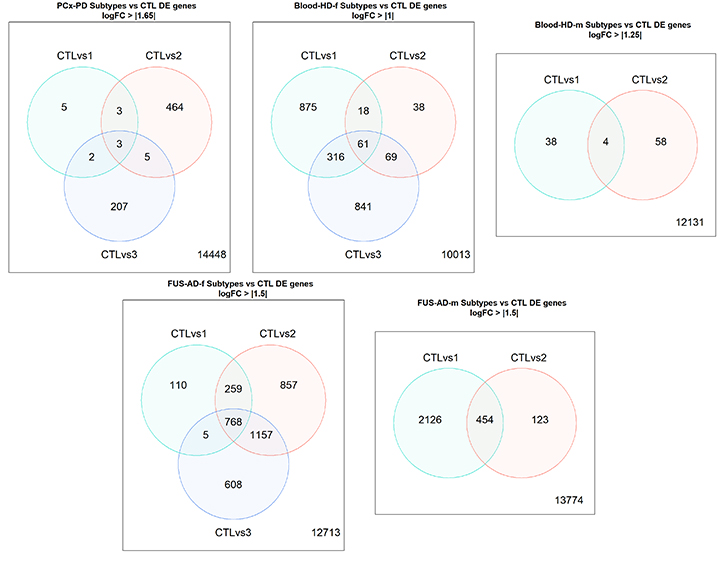
\includegraphics[width = 15cm]{Figures/subtype-venn.jpg}}
\caption{Venn diagrams for comparison of differentially expressed genes of each molecular subtype.}
\label{fig:venn-subtypes}
\end{figure}

\textbf{Blood-HD.} Moving on to Blood-HD-f, subtype 1 and subtype 3 resulted with more than 800 unique DEGs, while S2 obtained around 40. Furthermore, S1 and S3 shares 316 DEGs. The aforementioned suggests that S1 and S3 may have a more distinct pathological mechanisms caused by the high number of DEGs than those of S2. The three heatmaps presented in Appendix \ref{DE-blood-hd-f} show a clear contrast between case and control samples. Even though, S2 has less DEGs than the other subtypes, a distinction between S2 samples and control samples can be seen.

As mentioned before, only two subtypes were identified for Blood-HD-m. Nonetheless, these two sutbypes only intercept on four DEGs. Subtype 1 obtained 38 unique DEGs, and S2 resulted with 58. Its important to highlight that the LFC threshold is higher than for its female counterpart. As it is expected in both heatmaps (Appendix \ref{DE-blood-hd-m}), the pattern of the case samples is less clear than the one appreciated for the control samples given the amount of DEGs.

\textbf{Fus-AD.} Continuing to Fus-AD-f database, Fig. \ref{fig:venn-subtypes} reports large numbers of sutbype DEGs; remarkable contrasts are expected in the heatmaps. The number of common DEGs among Subtype 2 and 3 (1925 genes) supposes there is a high similarity between them. Nevertheless, S1 shares more than a thousand genes with S2 and around 770 with S3. Additionally, in Appendix \ref{DE-fus-ad-f}, the heatmaps of S1 and S2 appear to have a homogeneous under-expressed block on the case section, as well as in over-expressed part but with some blue spots. In general, the case samples has less variance than control. S2 has a perfect contrast.

Finally, sutbype 1 of Fus-AD-m resulted in more than 2,000 unique DEGs which suggests a more serious pathophysiology. S2 obtained 123 particular DEGs with an intercept of 454 genes with S1. The above may imply an equivalence between the two molecular subtypes. On the other hand, analyzing the heatmaps in Appendix \ref{DE-fus-ad-m}, it can be seen an uniform case block for S1, however, some samples do not resemble to neither control or case patterns. Same happens in S2 heatmap. In summary, both graphs contains a very clear contrast between case and control samples, which was foreseeable with the number of DEGs.

The last inference of this section belongs to the comparison of DEGs between distinct tissues with the same diseases, or similar tissues with different conditions. Observing the first Venn diagrams of Fig. \ref{fig:common-tissues-up} and \ref{fig:common-tissues-down}, only 52 over-expressed genes are shared among PD and HD in the prefrontal cortex, whereas, 151 under-expressed genes are common between these two conditions. In total, PD and HD share more than 200 DEGs in this tissue. Nevertheless, HD has 300 unique up-regulated and 468 down-regulated genes, which may suggest a more drastic change in the biologic pathways for this disease than for PD (92 and 88 genes, respectively).

\begin{figure}[!ht]
    \centerline{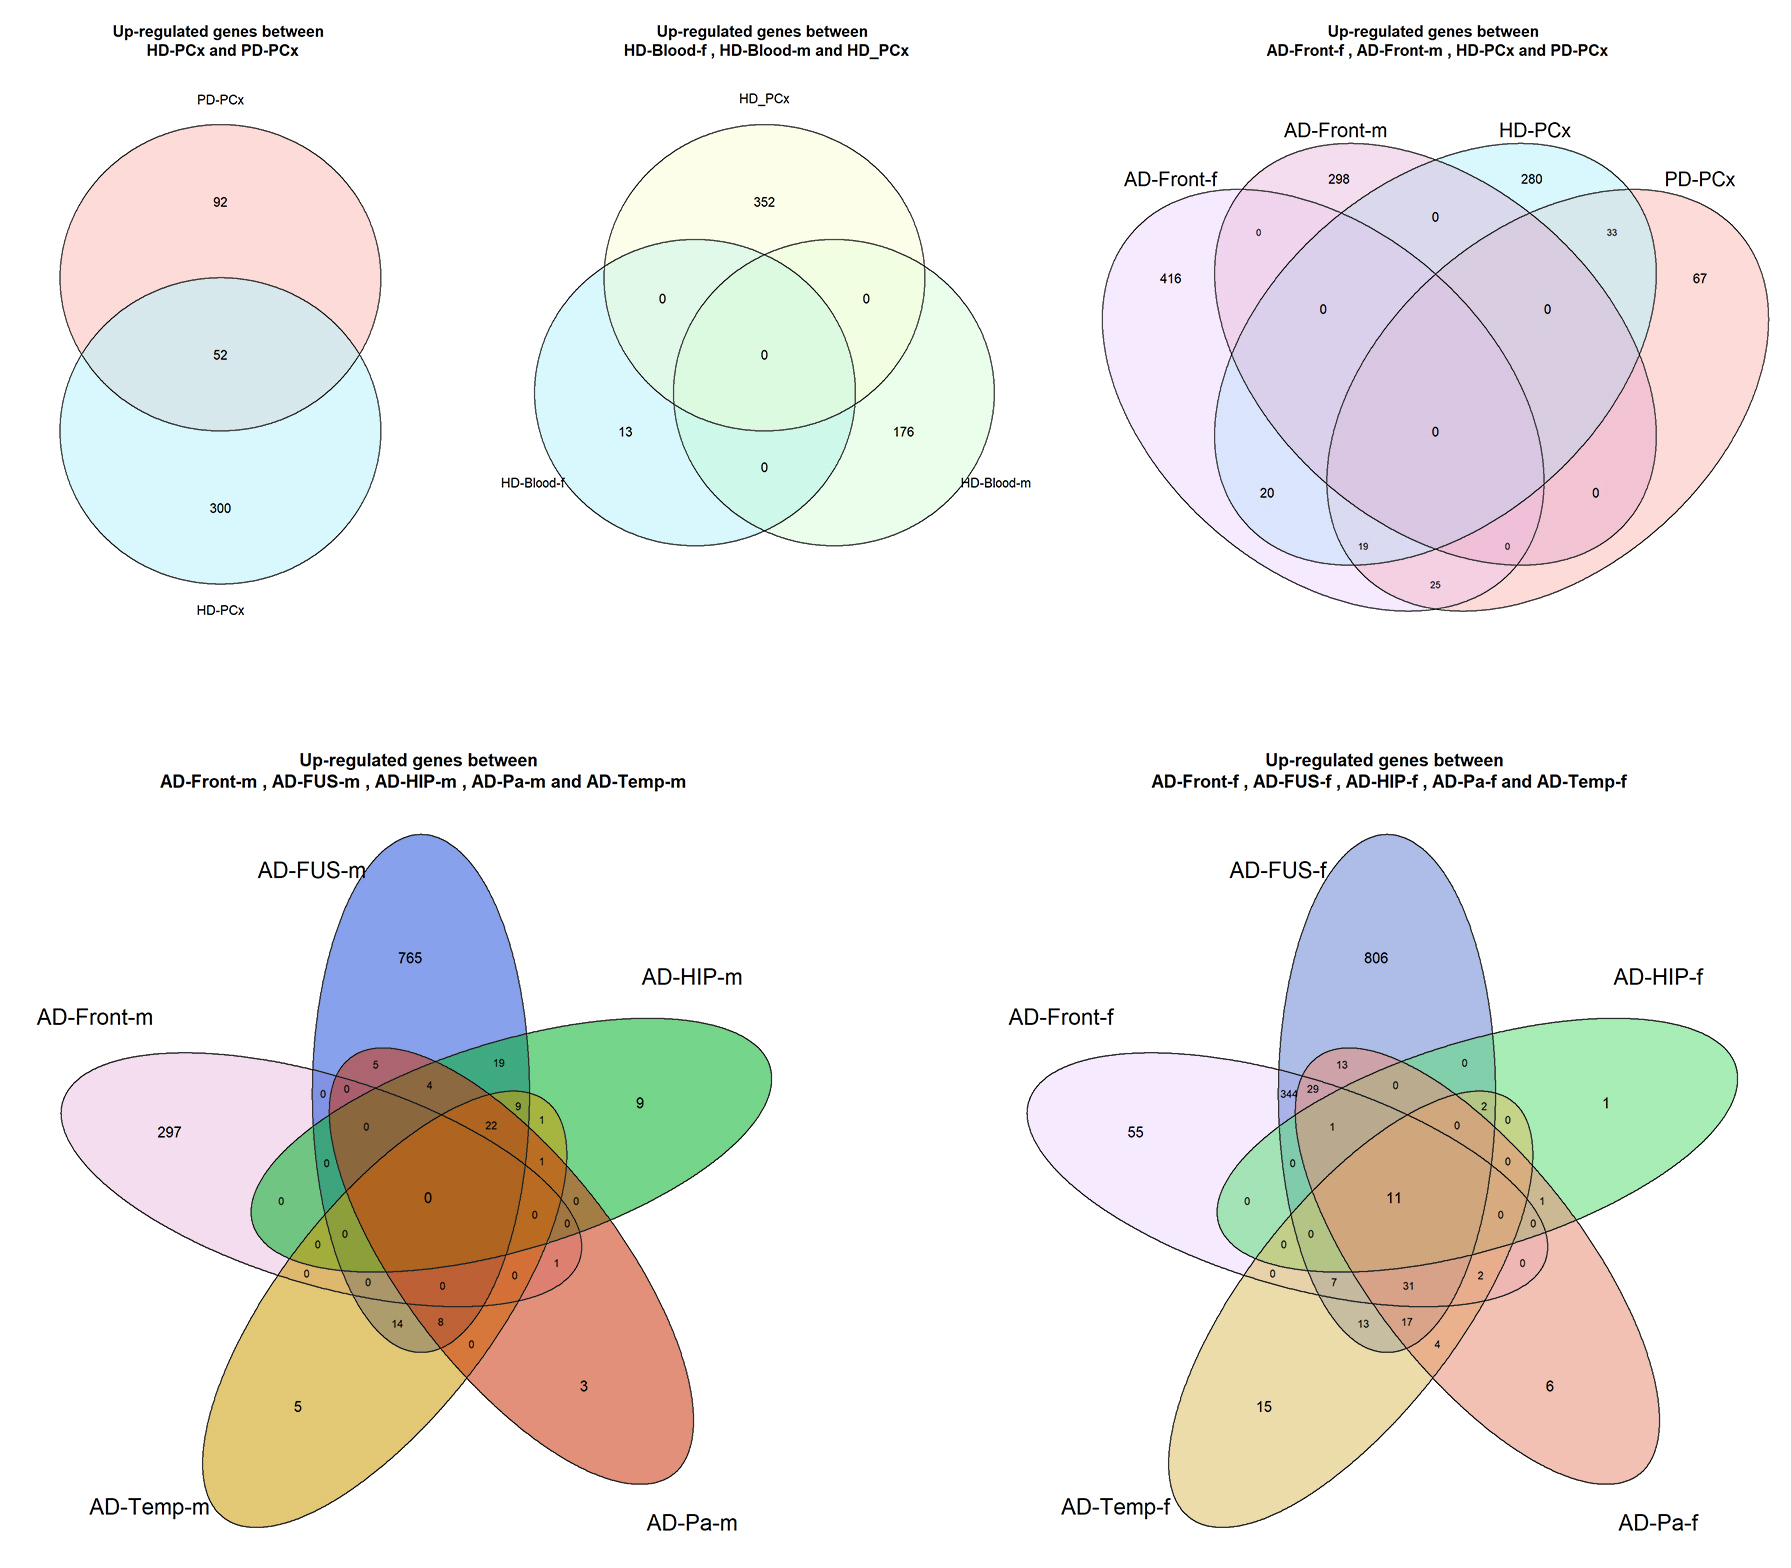
\includegraphics[width=10cm]{Figures/common-tissue-up-col.jpg}}
    \caption{Common up-regulated differentially expressed genes between tissues.}
\label{fig:common-tissues-up}
\end{figure}
    
\begin{figure}[!ht]
    \centerline{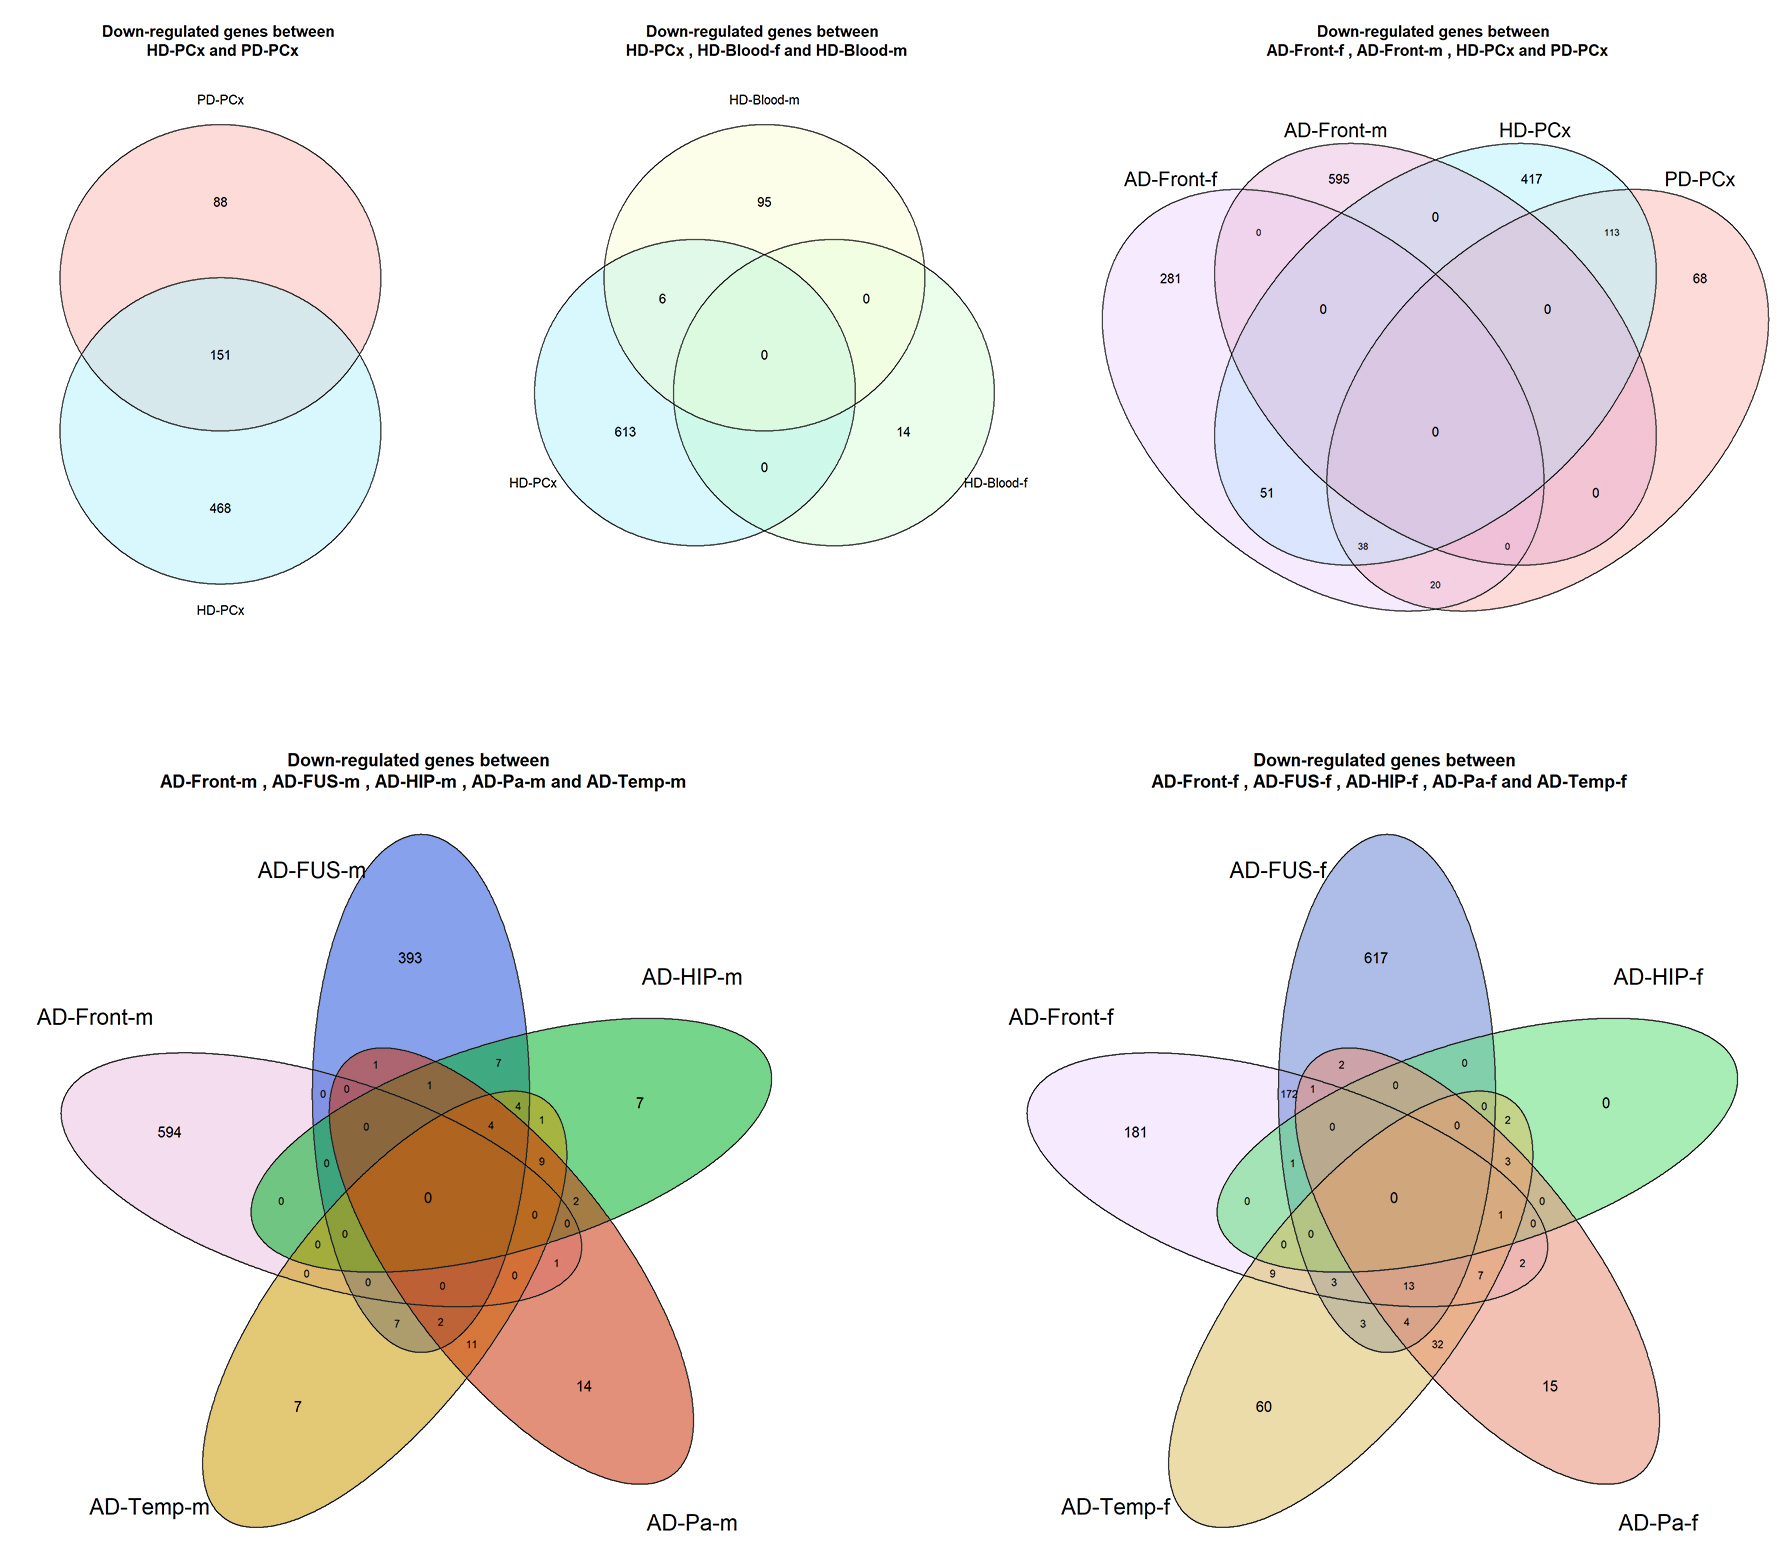
\includegraphics[width=10cm]{Figures/common-tissue-col.jpg}}
\caption{Common down-regulated differentially expressed genes between tissues.}
\label{fig:common-tissues-down}
\end{figure}

For the second diagrams of the figures, the comparisons among Blood-HD datasets and PCx-HD are shown. Interestingly, just six down-regulated genes are shared between PCx-HD and Blood-HD-m. The aforementioned may imply that blood does not resemble the alterations occurring in HD. Also, the magnitude of the altered genes of PCx-HD is far larger than the blood samples which supports the above idea. 

Furthermore, the comparison between similar tissues was done for the three conditions. As it can be seen in Fig. \ref{fig:common-tissues-up}, the three diseases do not have any gene in common, as well as in Fig. \ref{fig:common-tissues-down}. However, it is interesting to see that PCx-HD shares around 40 up-regulated and 90 down-regulated genes with Front-AD-f, while zero genes are intercepted with the male set. This could have suggested that PCx-HD was formed with a majority of female samples, but PCx-PD also shares around 100 DEGs with the female dataset, and it is known that PCx-PD contains 80\% of male samples. Moreover, as mention before, Front-AD-f and Front-AD-m does not have genes in common since they appear to be inverted.

Lastly, the interpretation of the relation among AD samples in varied tissues is given according to the bottom Venn diagrams of the two figures. It is interesting to observe that the male frontal tissue does not share any DEG with the other tissues, except for one under-expressed gene with parietal. However, Front-AD-f behaves differently, it has similarities with fusiform gyrus, and some others with the parietal and temporal lobes. Nonetheless, what is more interesting is the likeliness of these four diagrams. The tissues which are similar to other according on the number of common DEGs are the same between female and male, and the corresponding direction. In Table \ref{tab:eq-tissues}, the relation between tissues is shown. As it can be observed, the only divergence among the sexes is the frontal tissue.

\begin{table}[!ht]
\centering
\caption{Tissues similarities according to the number of differentially expressed genes.}
\label{tab:eq-tissues}
\begin{tabular}{ll|ll}
\hline
 & \multicolumn{1}{c|}{\textbf{Reference}} & \multicolumn{1}{c}{\textbf{Female}} & \multicolumn{1}{c}{\textbf{Male}} \\ \hline
\textbf{Up}   & Fusiform    & Frontal  & Hippocampus           \\
              & Parietal    & Fusiform & Fusiform              \\
              & Temporal    & Fusiform & Fusiform              \\
              & Hippocampus & Fusiform & Fusiform              \\
              & Frontal     & Fusiform & \multicolumn{1}{c}{-} \\ \hline
\textbf{Down} & Fusiform    & Frontal  & Temporal              \\
              & Parietal    & Temporal & Temporal              \\
              & Temporal    & Parietal & Parietal              \\
              & Hippocampus & Temporal & Temporal              \\
              & Frontal     & Fusiform & \multicolumn{1}{c}{-} \\ \hline
\end{tabular}
\end{table}

\section{Alternative Copy Number Variation}

After the DGE analysis was performed and the LFC of each gene was calculated, the alternative CNV analysis could be done. As mentioned in Section \ref{cnv-method}, the LFC averages of a moving 50 gene window (i.e. chromosome segments of 50 genes) were used to compute the CN. Its important to keep in mind that the reference of the contrast were the case conditions, except for the subtype comparison (control as reference). Moreover, the CNV results of the molecular subtypes were plotted in heatmaps, while the results of the datasets are given in CNV plots (Appendix \ref{cnvplots}).

\sloppy
\textbf{PCx-PD.} Briefly, the CNV plot of PCx-PD presented in Appendix \ref{cnvplots} shows an over-expression on chromosome 17 and 19. However, the mean-lines tend to go down the graph. Additionally, in order to compare the CN expression of the subtypes and the control, a heatmap was generated (Fig. \ref{fig:cnv-hm-pd}). As it can be seen, control group has a clear block which can be used to contrast with subytpes. The most evident contrast between control and subtype 1 happens somewhere in the region of chromosome 1 until 8, and 16 till X; where control is down-regulated, S1 is up-regulated, and vice-versa. On the other hand, subtype 2 looks alike to S1, and S3 appears to have a more mixed color, although some blocks that differ from control can be appreciated.

\begin{figure}[!ht]
    \centerline{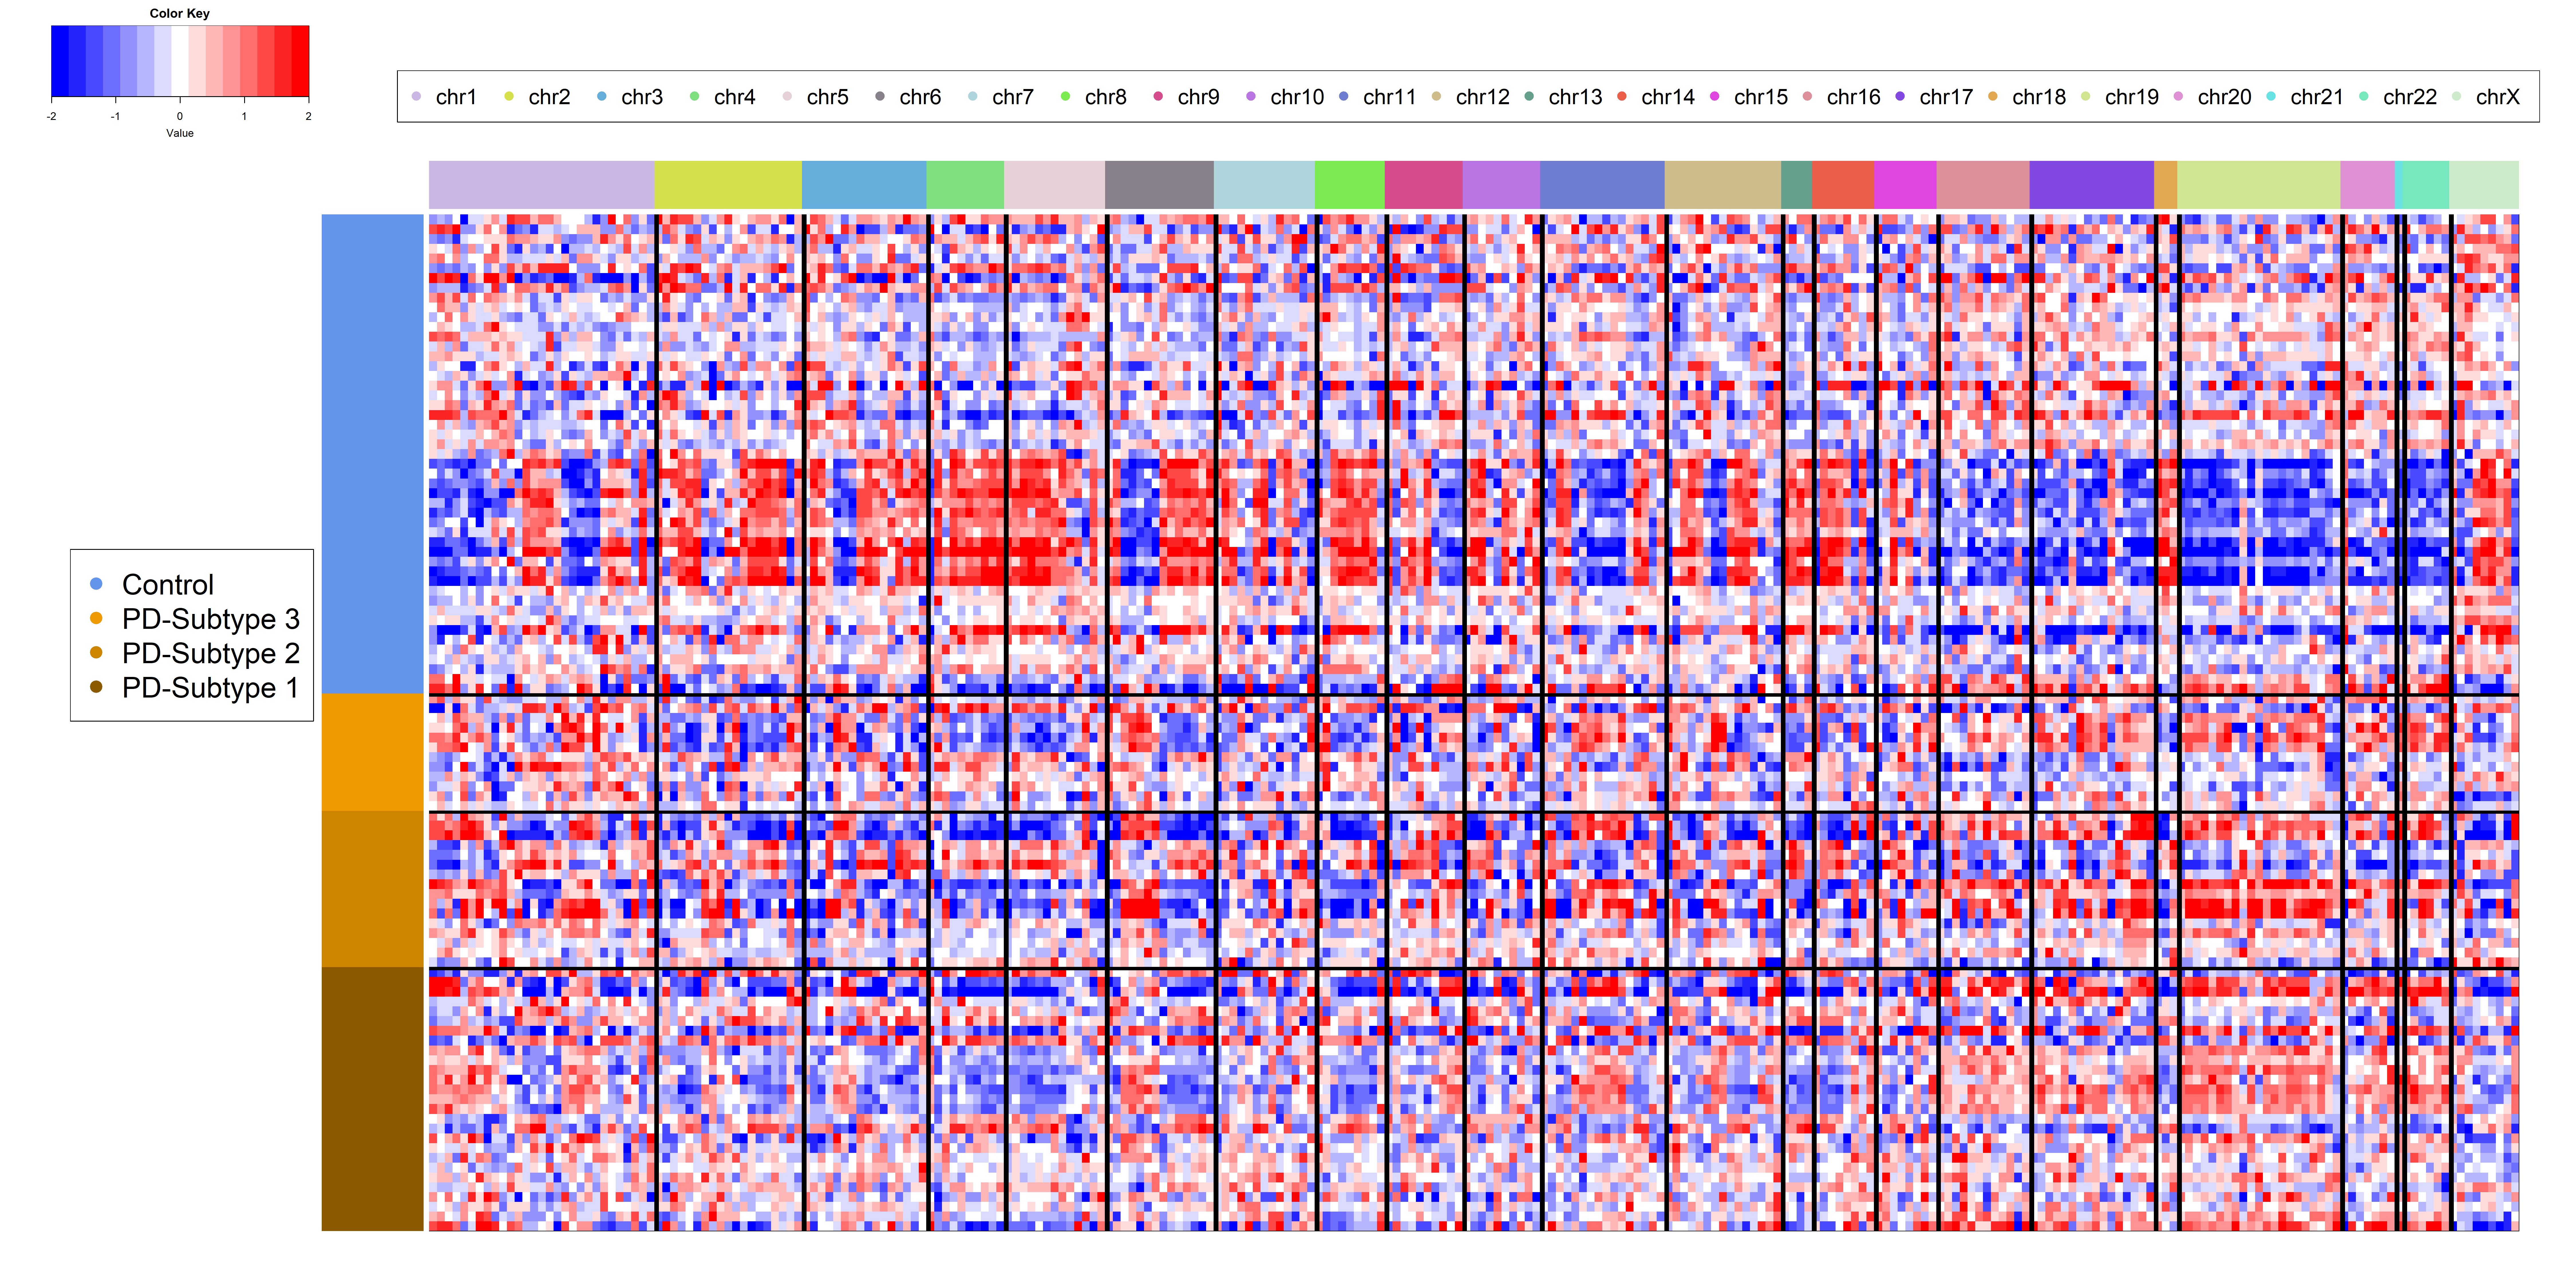
\includegraphics[width = 15cm]{Figures/CNV/cnv-pd.png}}
\caption{Heatmap for the comparison of CNV between control and molecular subtypes of PCx-PD.}
\label{fig:cnv-hm-pd}
\end{figure}

\textbf{PCx-HD.} In Appendix \ref{fig:cnv-pcx}, it seems that there is no relevant changes in the mean-line for PCx-HD. However, there are some segments (dots on the graph) which have an extreme expression. These segments are located in the positive direction in chromosome 1, 6, 11, 16 and 19, and in the negative direction in chromosome 5.

\textbf{Blood-HD.} The female set CNV plot (see Appendix \ref{fig:cnv-blood}) suggests that chromosome 17, 19 and 20 have a high number of up-regulated genes, and chromosome 5 has several down-regulated segments. For the male part, chromosome 2 to 5 have many over-expressed segments, specially chromosome 13. While chromosome 16, 17, 19 and 22 tend to go down. When both sexes are compared, more male segments are differentiated and with higher magnitude than in the female set; which make sense with the results in Table \ref{tab:de-genes}. Furthermore, in the subtype heatmap of Blood-HD-f in Fig. \ref{fig:cnv-hm-blood}, it can be appreciated that control and subtype 1 contrast in chromosome 4, 5, 16, 17, and 19. Subtype 2 seems to have no relevant changes, and S3 appears to have the same pattern as S1. Moreover, the male heatmap shows a contrast among S2 and control at chromosome 3, 4, 5, and 16 till 22. S1 seems to have 2 patterns (half above and half below), but according to NMF, three molecular subtypes were less possible than two.

\begin{figure}[!ht]
    \centerline{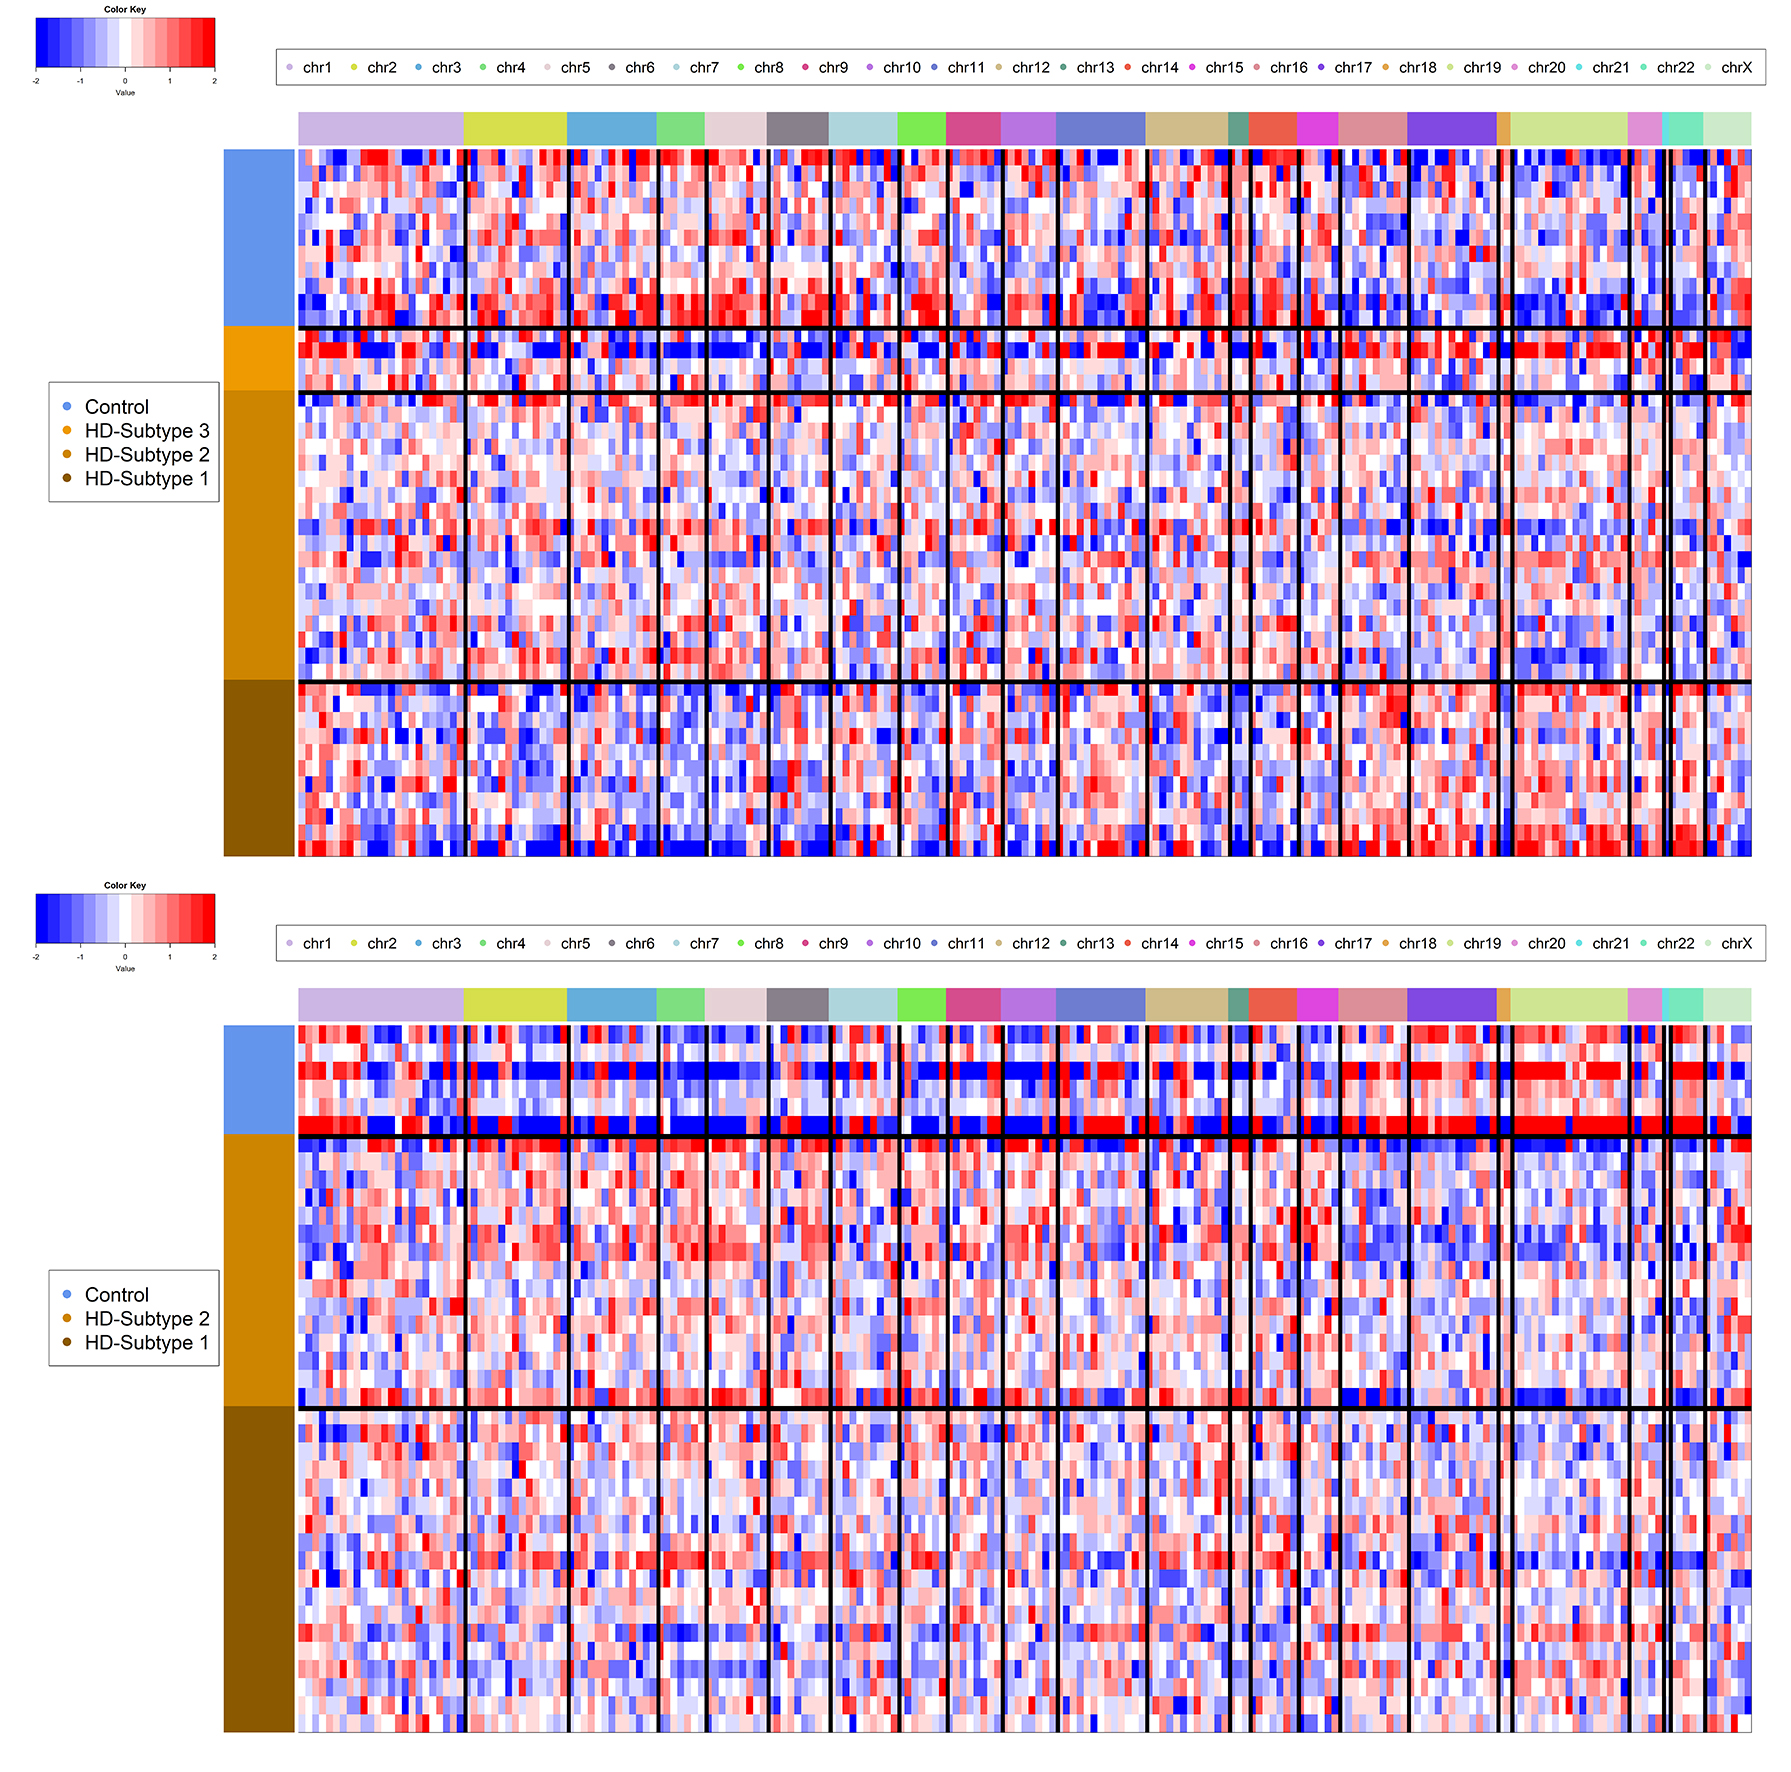
\includegraphics[width = 15cm]{Figures/CNV/cnv-blood.jpg}}
\caption{Heatmap for the comparison of CNV between control and molecular subtypes of Blood-HD.}
\footnotesize Top female, bottom male.
\label{fig:cnv-hm-blood}
\end{figure}

\textbf{Pa-AD.} In CNV plot of Pa-AD-f in Appendix \ref{fig:cnv-pa}, some chromosomes get the attention due to the several over-expressed segments: chromosome 16, 17, 19 and 22. Also, chromosome X is down-regulated and contains one point which is extremely down. In general, the chromosome expressions tend to be under-expressed, according to the mean-lines. In addition, the same tendency can be appreciated in the graph of the male counterpart: all chromosome are inclined to go down, chromosome X has the acutest negative value, and chromosomes 16 to 22 are over-expressed. The biggest change between the sexes is in chromosome 6.

\textbf{Temp-AD.} In general, both sexes are similar except for the magnitude, which it seems that in the female samples is a bit higher (see Appendix \ref{fig:cnv-temp}). Then again, the chromosomes tend to go to the negative values. The larger alterations occurred somewhere in the region of chromosomes 2 till 8, and 16 to 19, and X; the highest segments are located in chromosomes 16 and 19, while the lowest is in chromosome X.

\textbf{Hip-AD.} Looking at the mean-lines of Appendix \ref{fig:cnv-hip}, the changes among female and male sets are very similar; the female alterations are less differentiated than those of the male set. Another exception is that the mean-line of chromosome 10 in female is up-regulated, whereas in male is down-regulated. Similar to other datasets, the chromosomes are inclined to the negative side. The most under-expressed segments are located in chromosomes 2, 4, 5, 8, and X; the latter contains the lowest point. On the other hand, the most up-regulated chromosomes are 16, 17, 19, and 22; the highest point is at chromosome 19.

\textbf{Front-AD.} In the CNV plots of Appendix \ref{fig:cnv-front}, the first aspect to notice is that the female and male patterns appear to be inverted (same idea of previous sections). While in female chromosomes 16, 17 and 19 go to the up direction, in male those chromosomes go down; the female chromosomes 8, 13, 18 and X are under-expressed, whereas in male are over-expressed. As the other datasets, the lowest point in female is located in X, and the highest in chromosome 6 and 17; the opposite happens in male CNV plots.

\textbf{Fus-AD.} Finally, Fus-AD results are plotted in Appendix \ref{fig:cnv-fus}. The female set obtained five chromosomes with up-regulated expression (1, 11, 16, 17, and 19) and two with down-regulated tendency (4 and X). For both sexes the mean-lines tend to go down, as in other tissues. Moreover, the male set has a resemblant pattern to that of the female. Lastly, the female subtpye heatmap (Fig. \ref{fig:cnv-hm-fus}) presents a defined contrast between control and S1 along the majority of chromosomes. Additionally, the difference is hard to notice for sutbype 2, but in chromosomes 19 and X is visible. Likewise, S3 has some clear contrasts only in chromosomes 5, 16, 17, 19, 20, and 22. For the male set, although S1 has a mixed pattern, a difference is appreciated in the first half of chromosome 6, as well as in chromosomes 19, 20 and X. On the other hand, S2 is more explicit and has a strong contrast with control samples: up for chromosomes 6, 16 to 22, and down for chromosomes 4, 5, half of 6, and 13.

\begin{figure}[!ht]
    \centerline{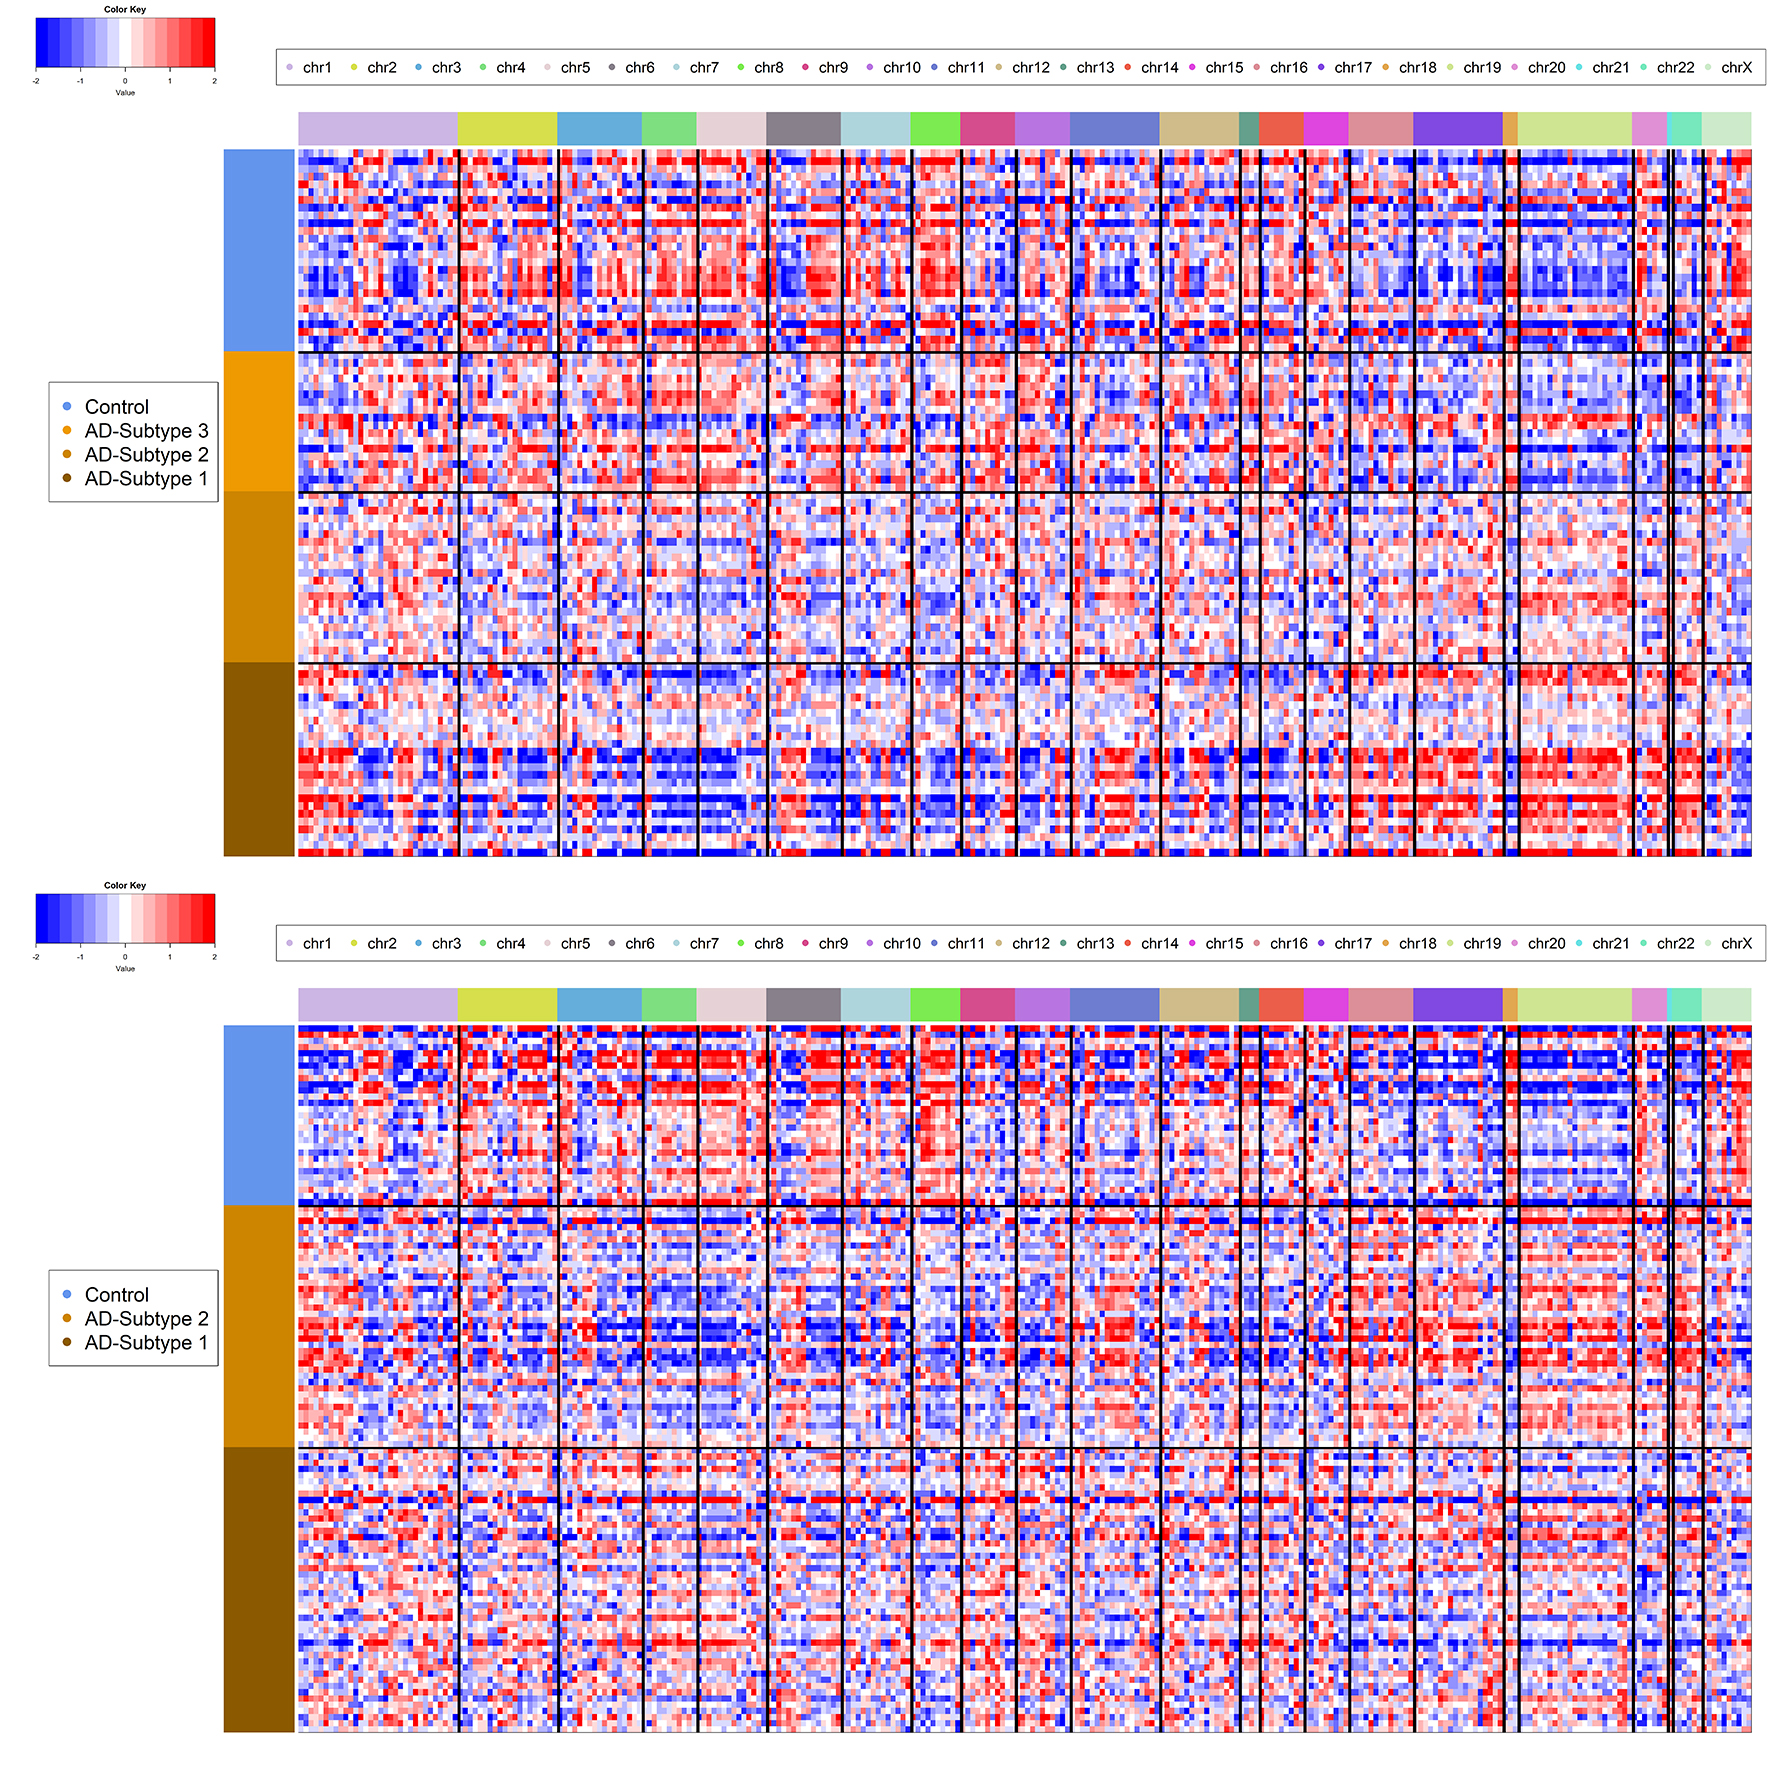
\includegraphics[width = 15cm]{Figures/CNV/cnv-fus.jpg}}
\caption{Heatmap for the comparison of CNV between control and molecular subtypes of Fus-AD.}
\footnotesize Top female, bottom male.
\label{fig:cnv-hm-fus}
\end{figure}

\section{Functional Analysis}

Functional analysis as an essential examination that allows to identify the altered pathways in which the DEGs are implicated. Hence, this analysis helps to understand the general pathophysiology of a disease. In Section \ref{path-method}, the steps of this analysis are explained. For the interpretation of the results only the bar and dot plot were used; the other type of visualizations generated are located in Appendix \ref{gsea-plots}. Keep in mind that all the changes in case vs control contrast are based on case, while the changes in subtype vs control are based on control.

\textbf{PCx-PD.} According to the 20 most significant pathways of the ORA analysis (Fig. \ref{fig:path-pxc-pd}), the DEGs of PCx-PD dataset are involved in immune system processes, response to bacteria, homeostasis, secretion, and neuropeptide signaling pathways. Whereas the GSEA results focused on terms associated with the brain, such as neuron synapse, substantia nigra development, and tau protein binding. In addition, pathways related to protein localization and cytosolic ribosome were obtained. 

\begin{figure}[ht]
    \centerline{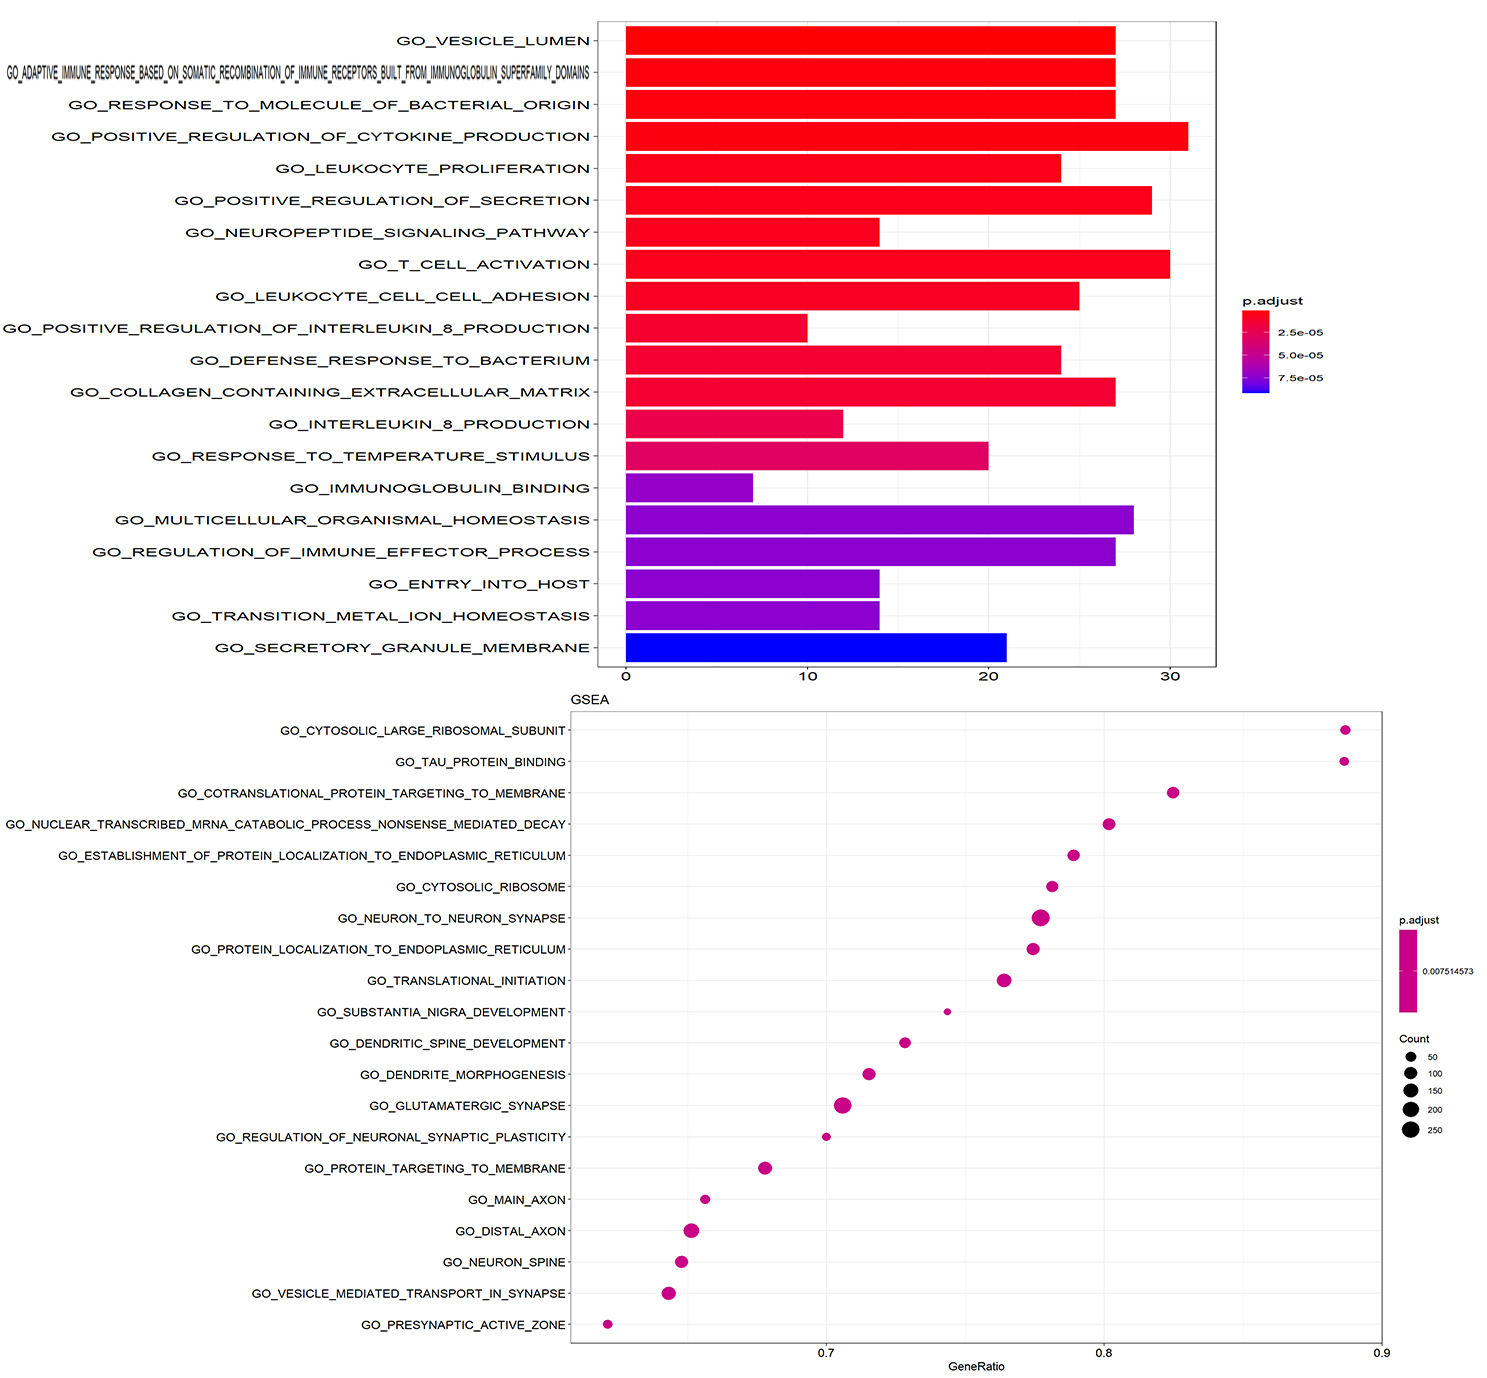
\includegraphics[width = 10cm]{Figures/Path/Path-PCx-PD.jpg}}
\caption{Visualization of over representation analysis and gene set enrichment analysis with a bar plot and dot plot, respectively, for PCx-PD.}
\label{fig:path-pxc-pd}
\end{figure}

Furthermore, the functional test for the molecular subtypes of PD resulted in the following. In Fig. \ref{fig:path-pd-sub}, subtype 1 only obtained 2 pathways with adjusted p-value of 0.036: protein folding chaperon, and neuropeptide hormone activity. S2 pathways are enclosed in ensheatment of neurons and synapse, membrane transporter and channels, oligodendrocyte development, glial cells, and myosin II binding (for muscle contraction); these pathways are more related to nervous system processes. The results for S3 can be summarized in extracellular matrix and collagen, and immune response and inflammation. Additionally, for GSEA, S1, S2 and S3 resulted with immune system processes and inflammation, while S1 and S3 have cardiovascularity development pathways. Moreover, S2 was enriched in gliogenesis, oligodendrocyte development, and ensheatment of neurons, similar to those obtained in ORA. S3 also resulted with extracellular matrix pathways.

\begin{figure}[!ht]%
    \centering
    \subfloat[\centering ORA for S1. ]{{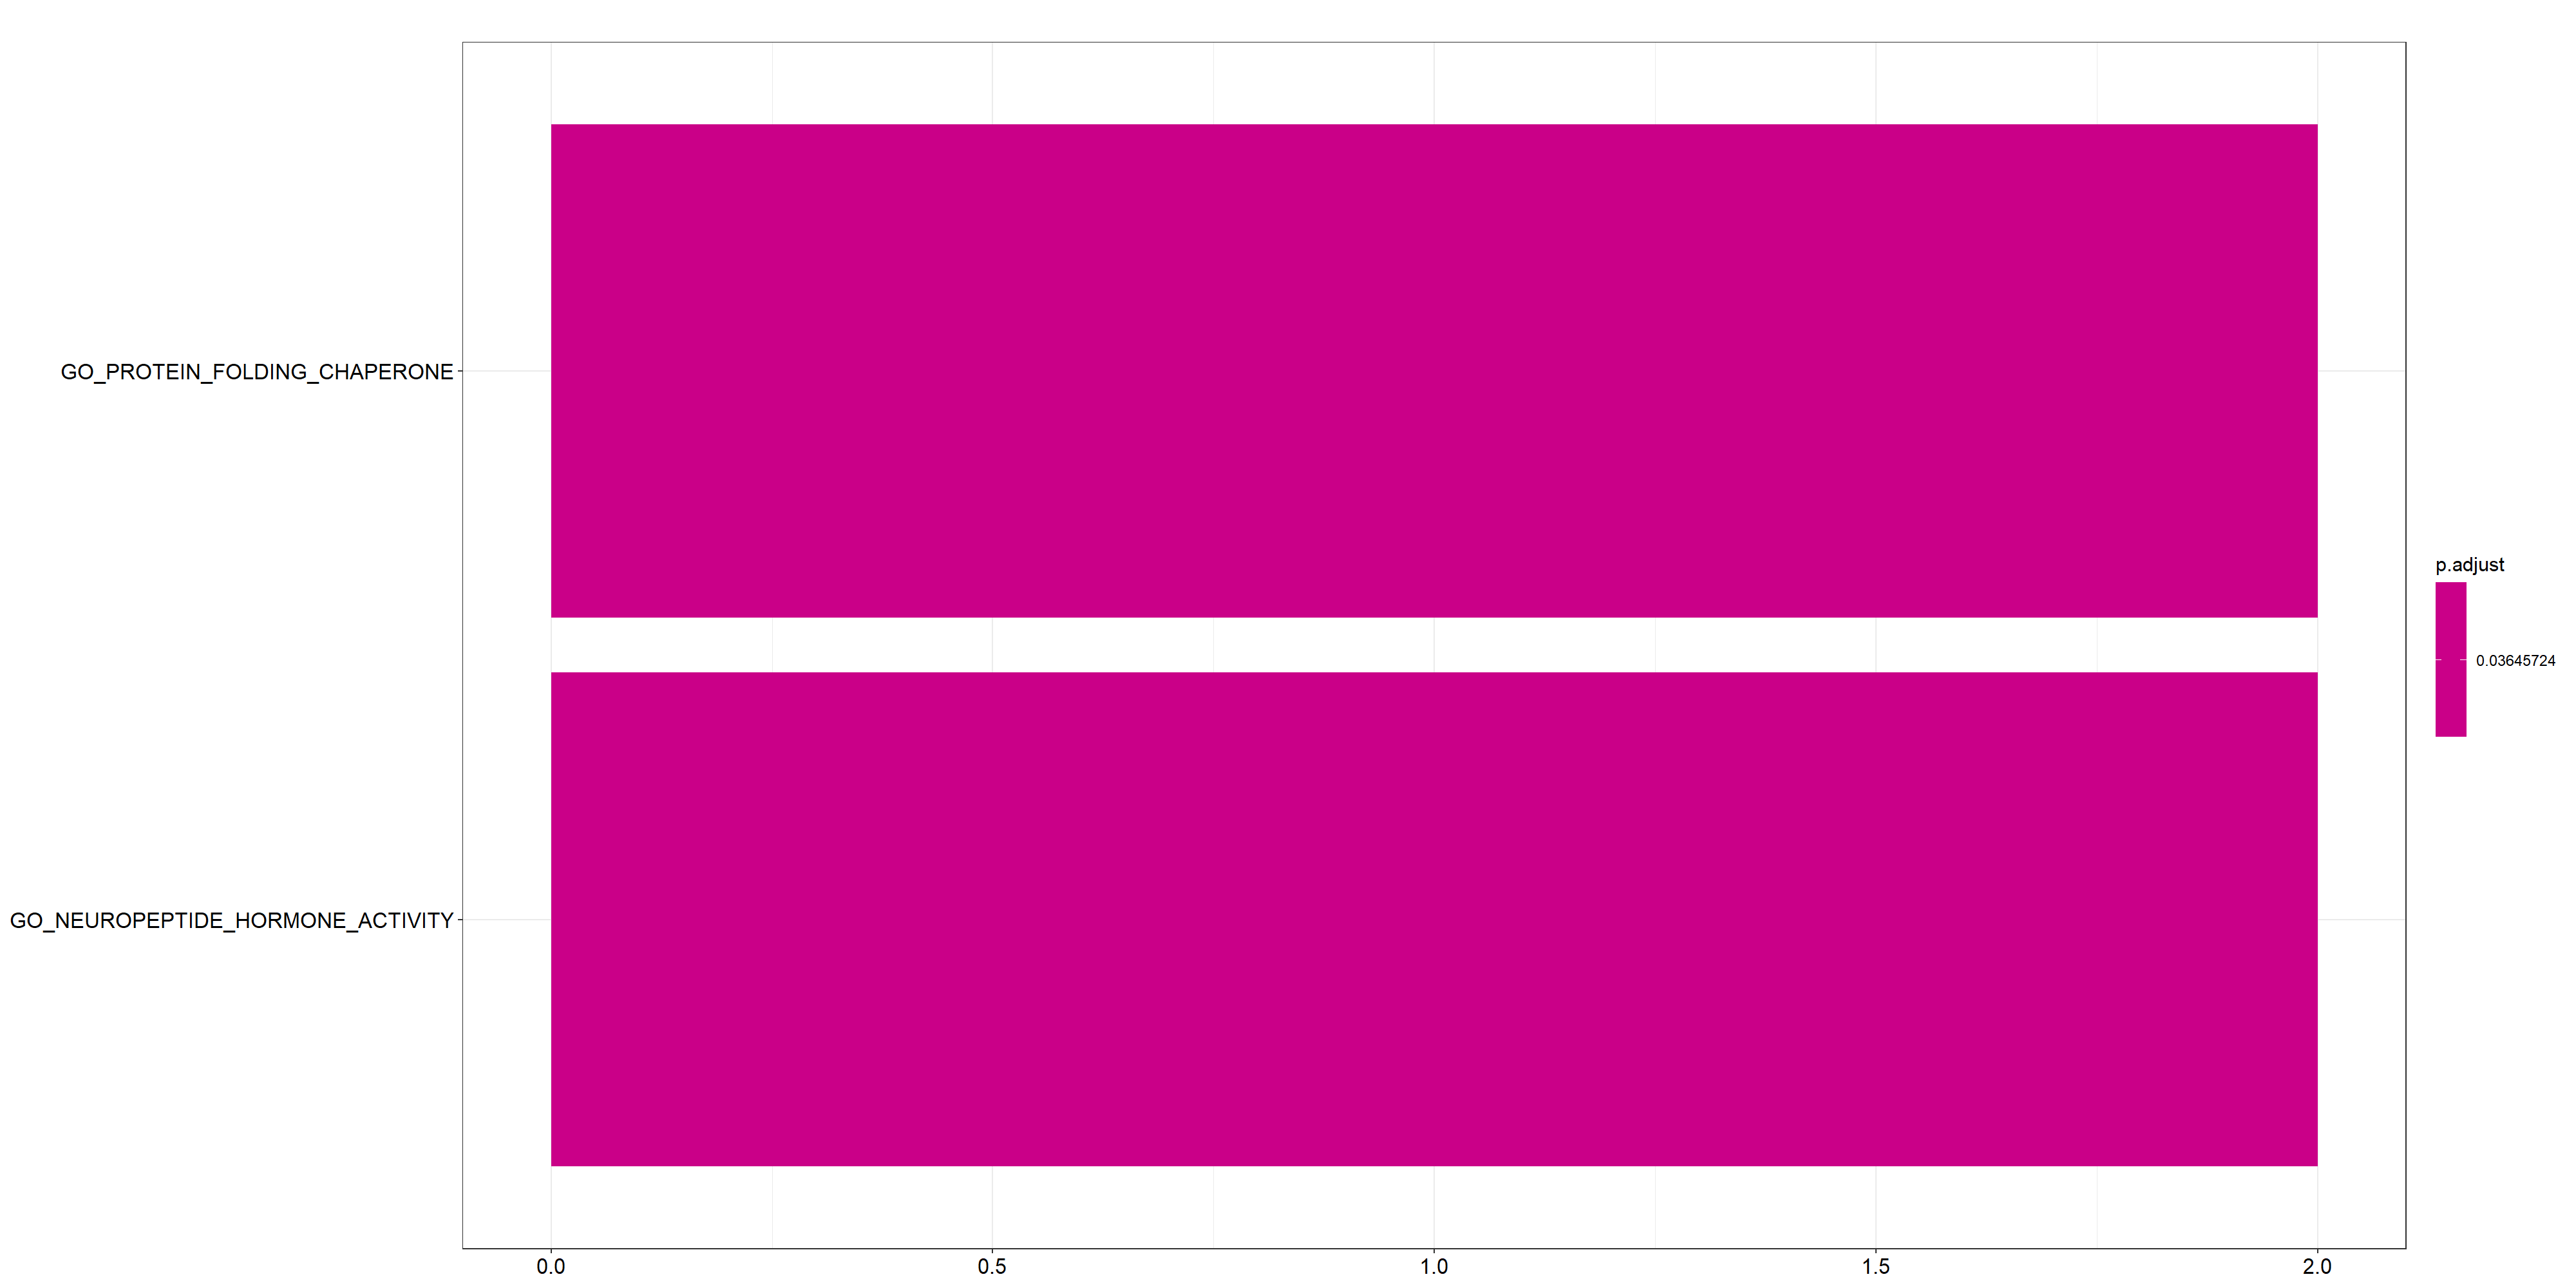
\includegraphics[width=5cm]{Figures/Path/CTLvs1_e_barplot.png} }}%
    \qquad
    \subfloat[\centering GSEA for S1. ]{{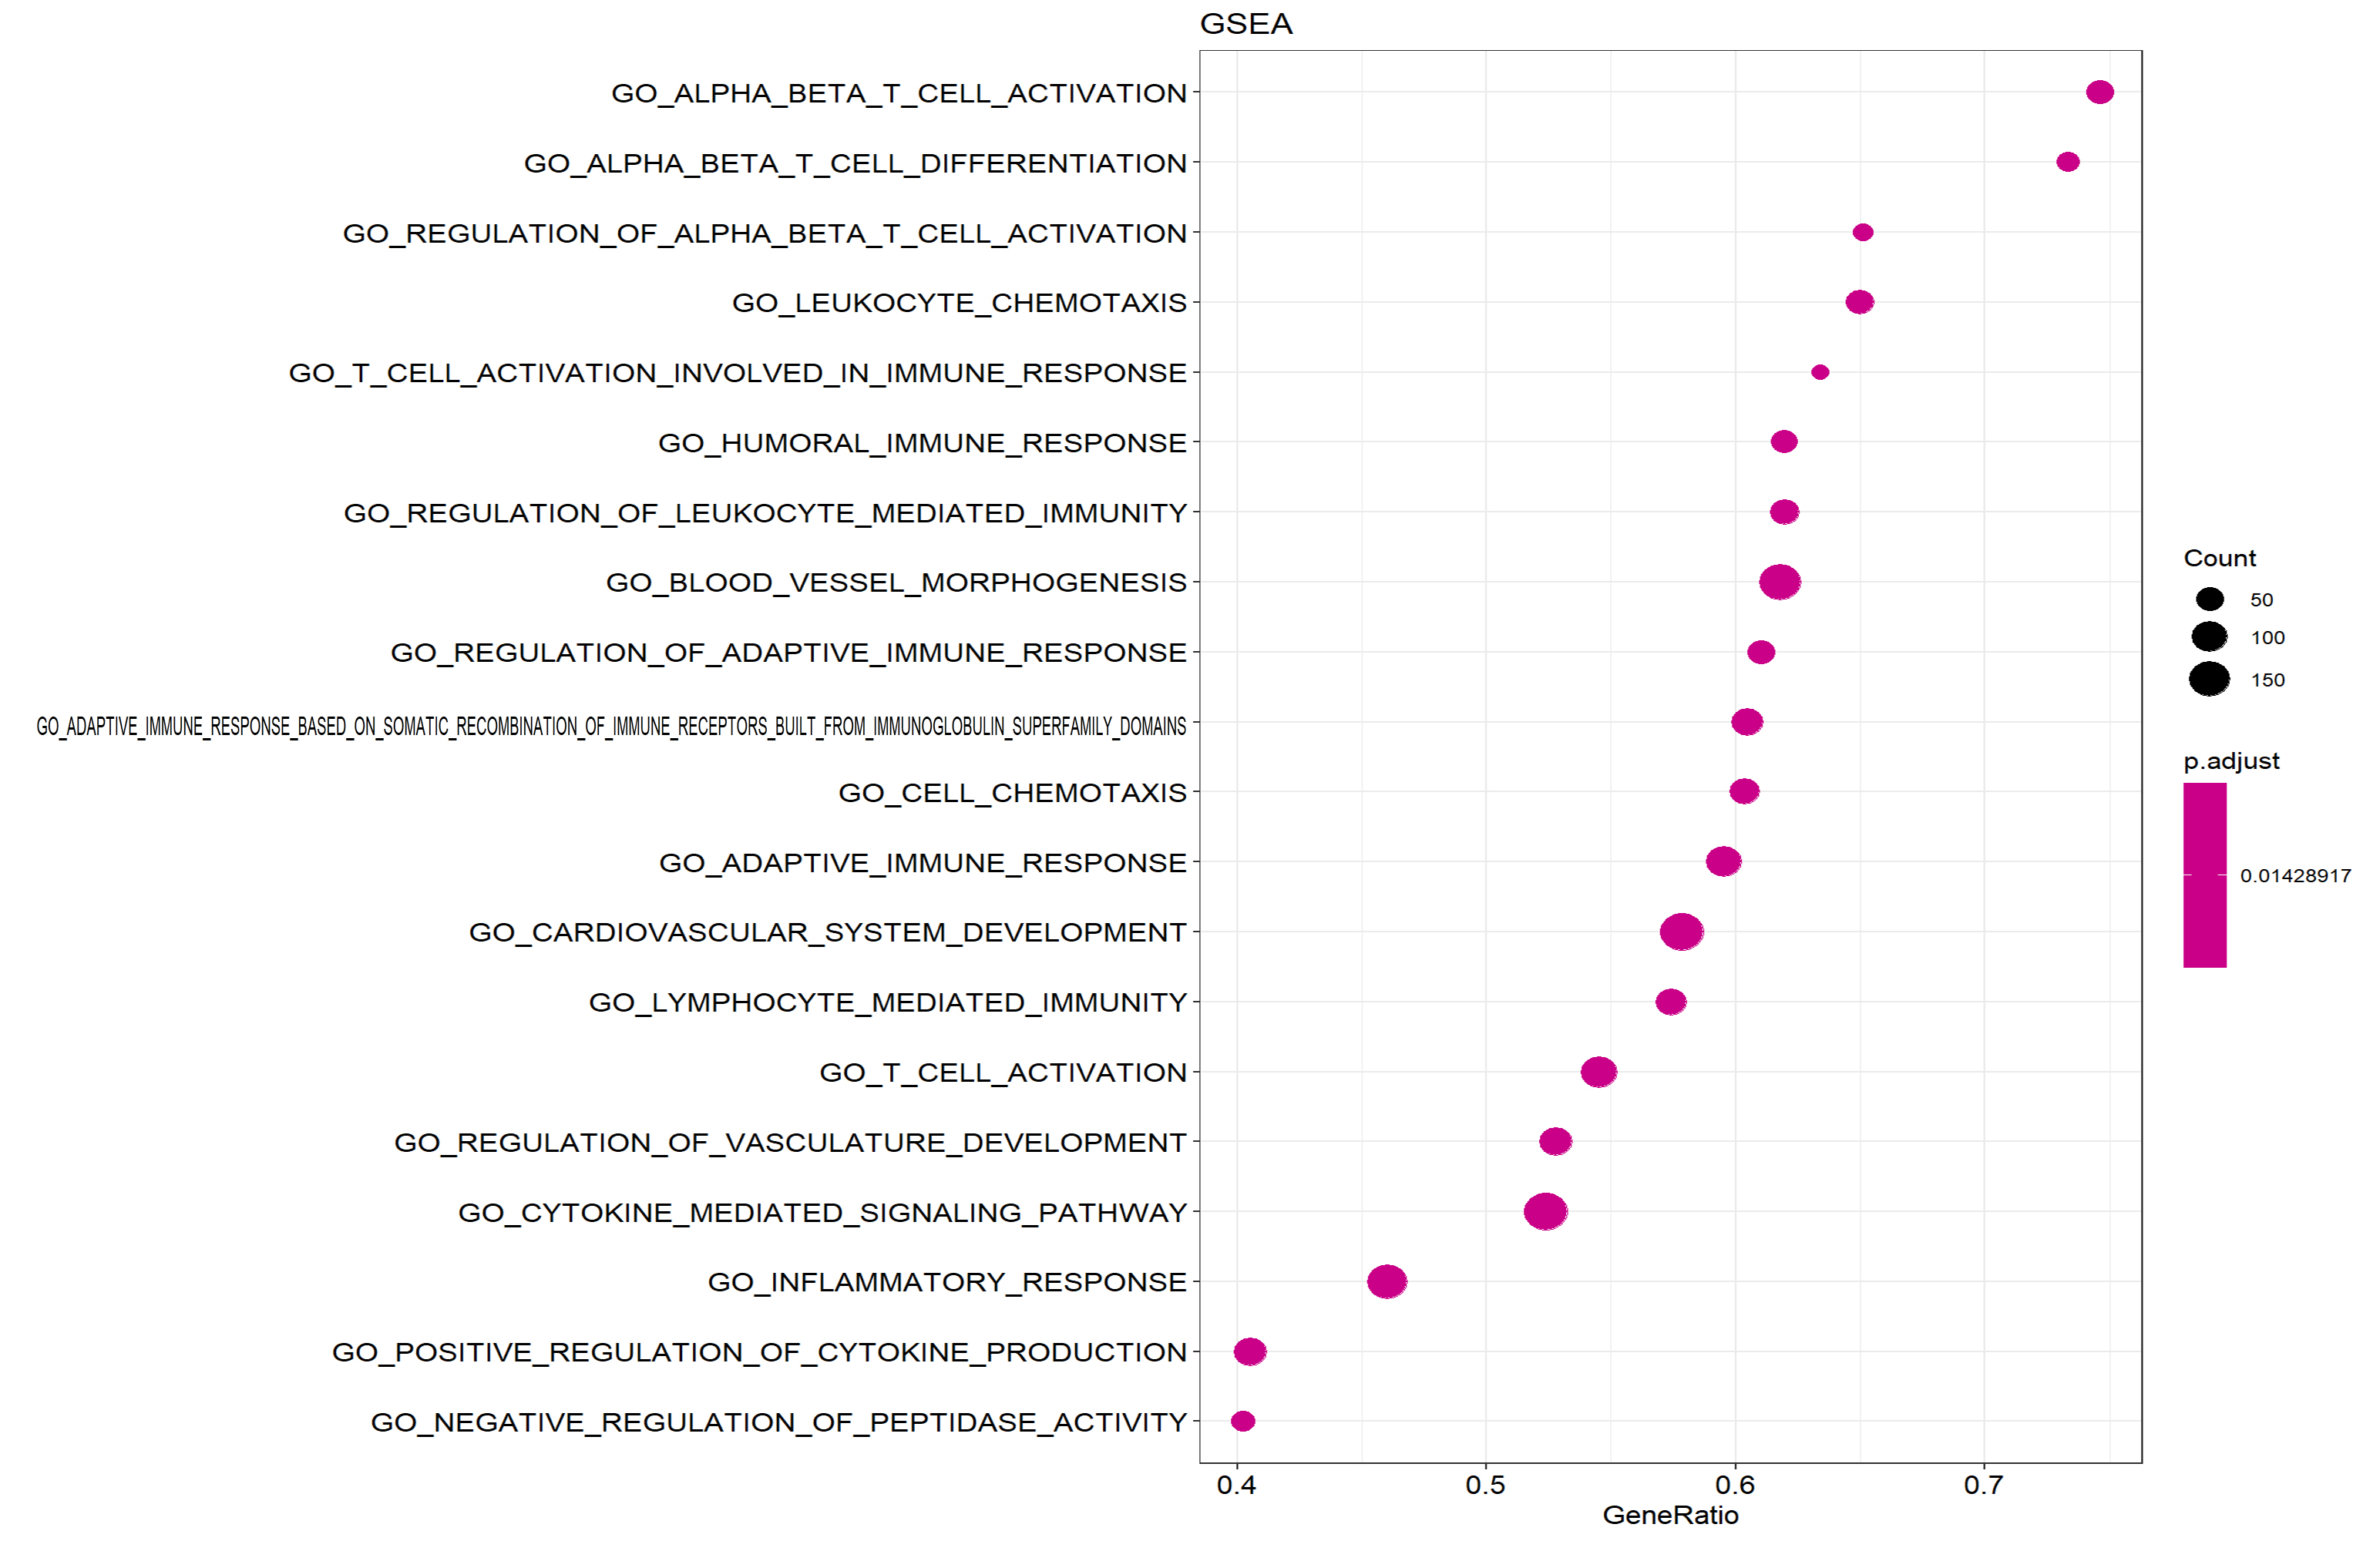
\includegraphics[width=5cm]{Figures/Path/dot-plot-s1.jpg} }}%
    \\
    \subfloat[\centering ORA for S2. ]{{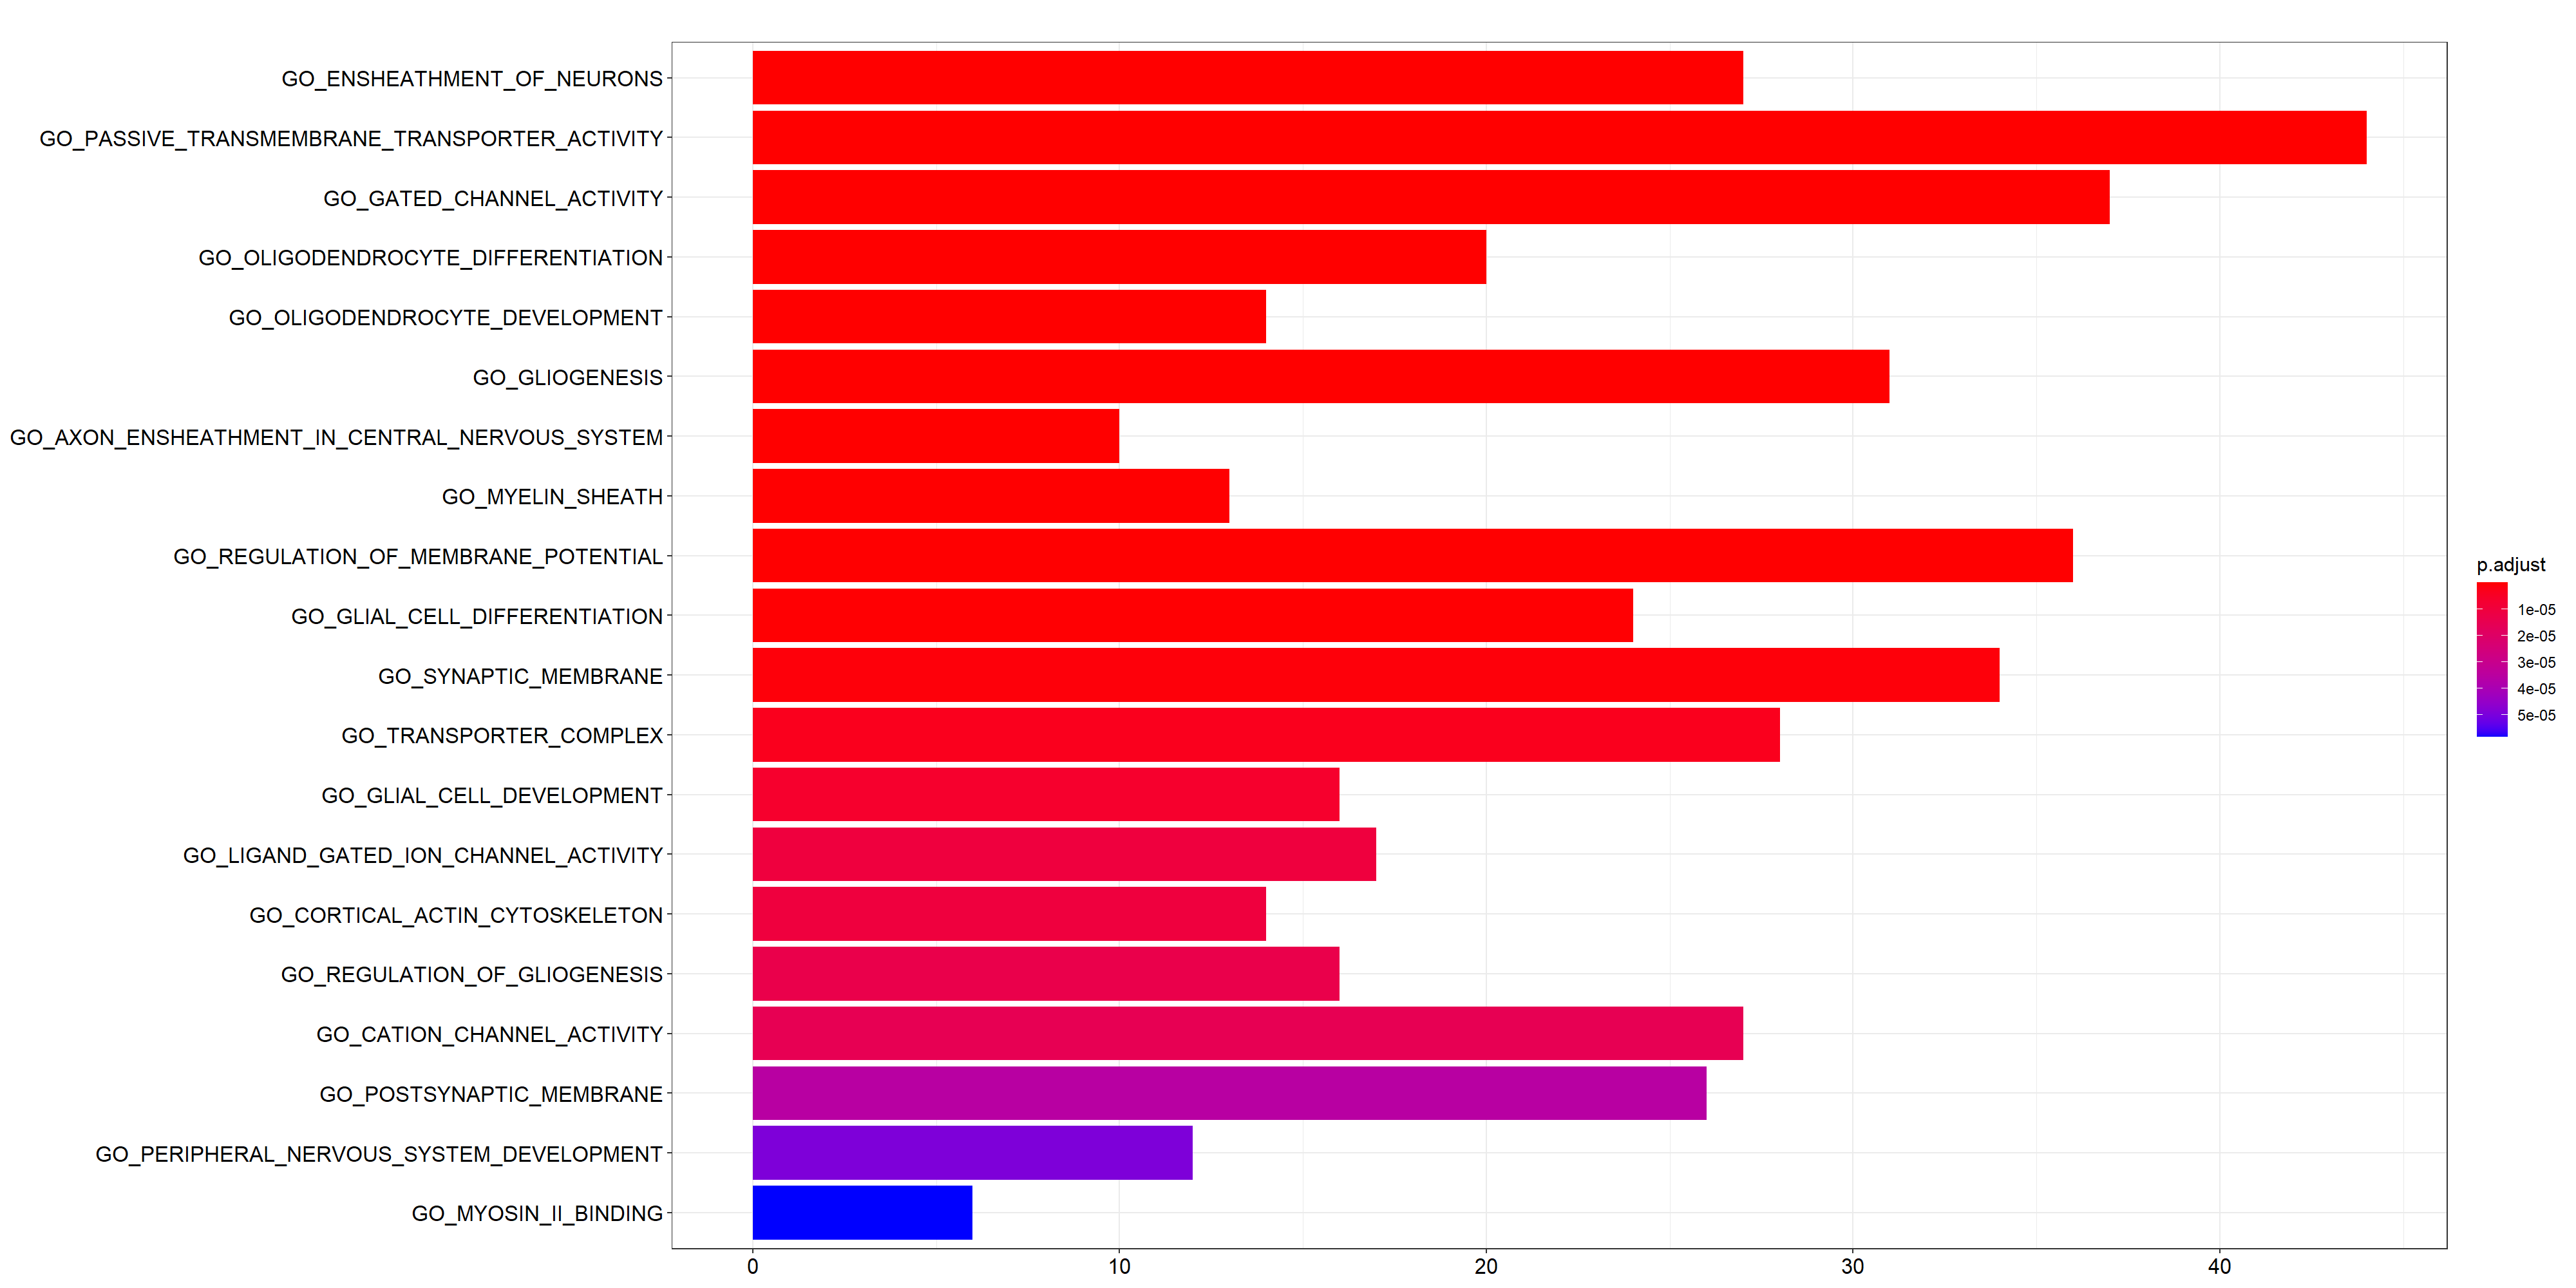
\includegraphics[width=5cm]{Figures/Path/CTLvs2_e_barplot.png} }}%
    \qquad
    \subfloat[\centering GSEA for S2. ]{{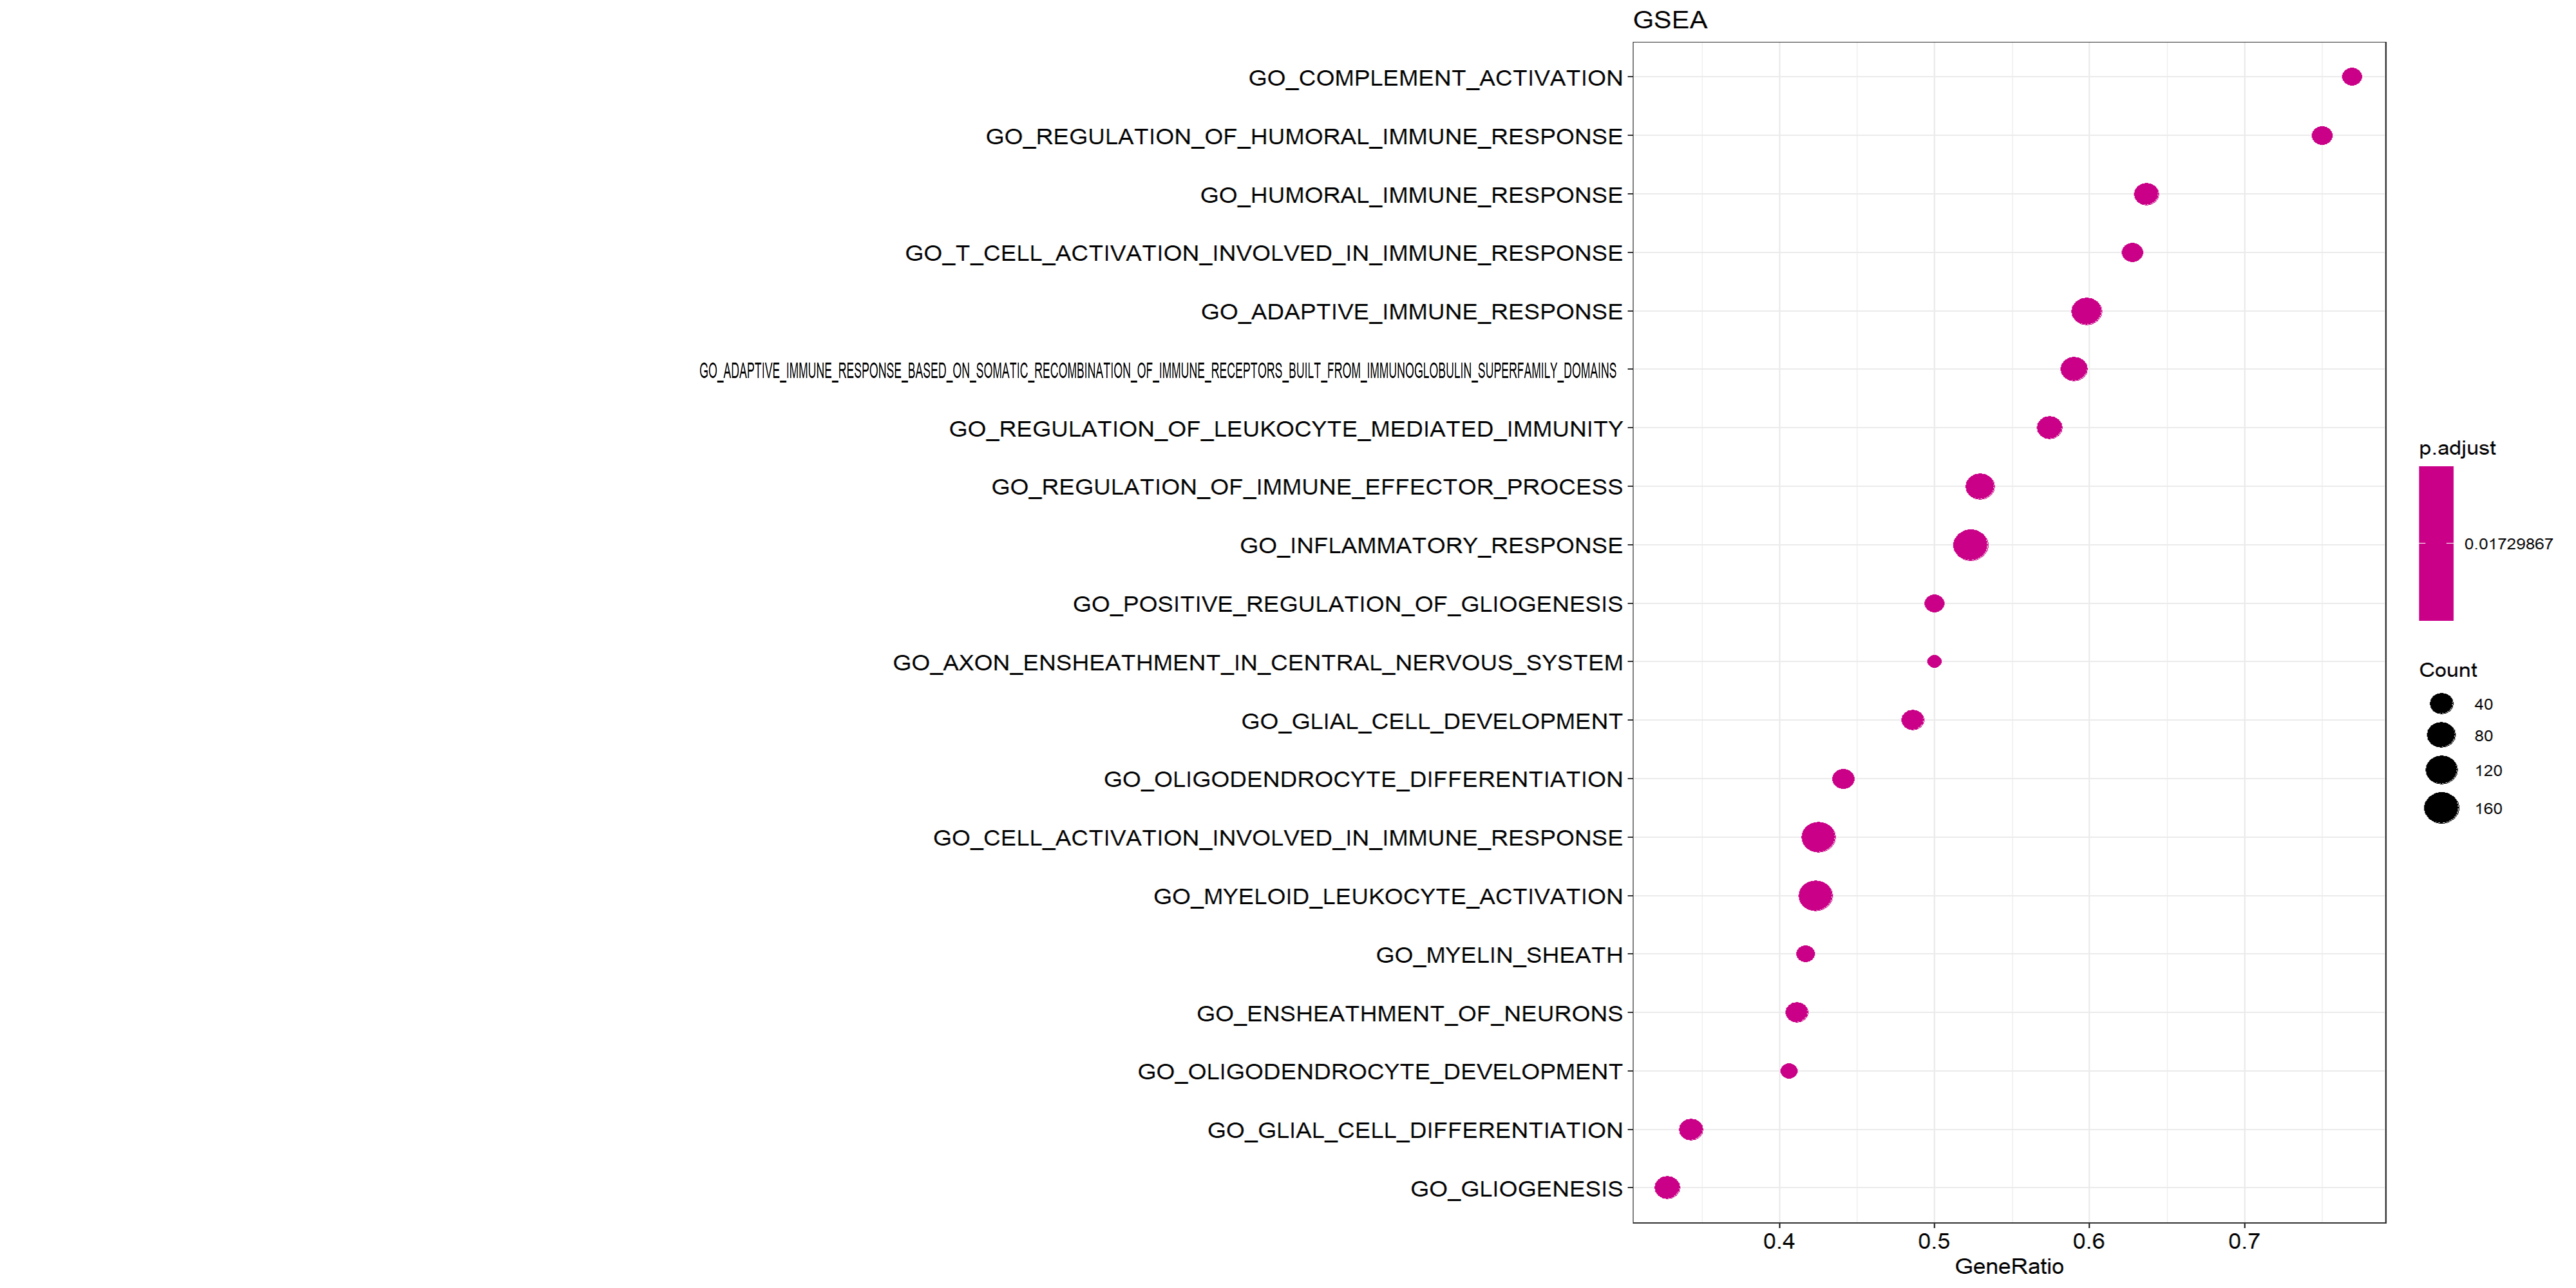
\includegraphics[width=5cm]{Figures/Path/dot-plot-s2.jpg} }}%
    \\
    \subfloat[\centering ORA for S3. ]{{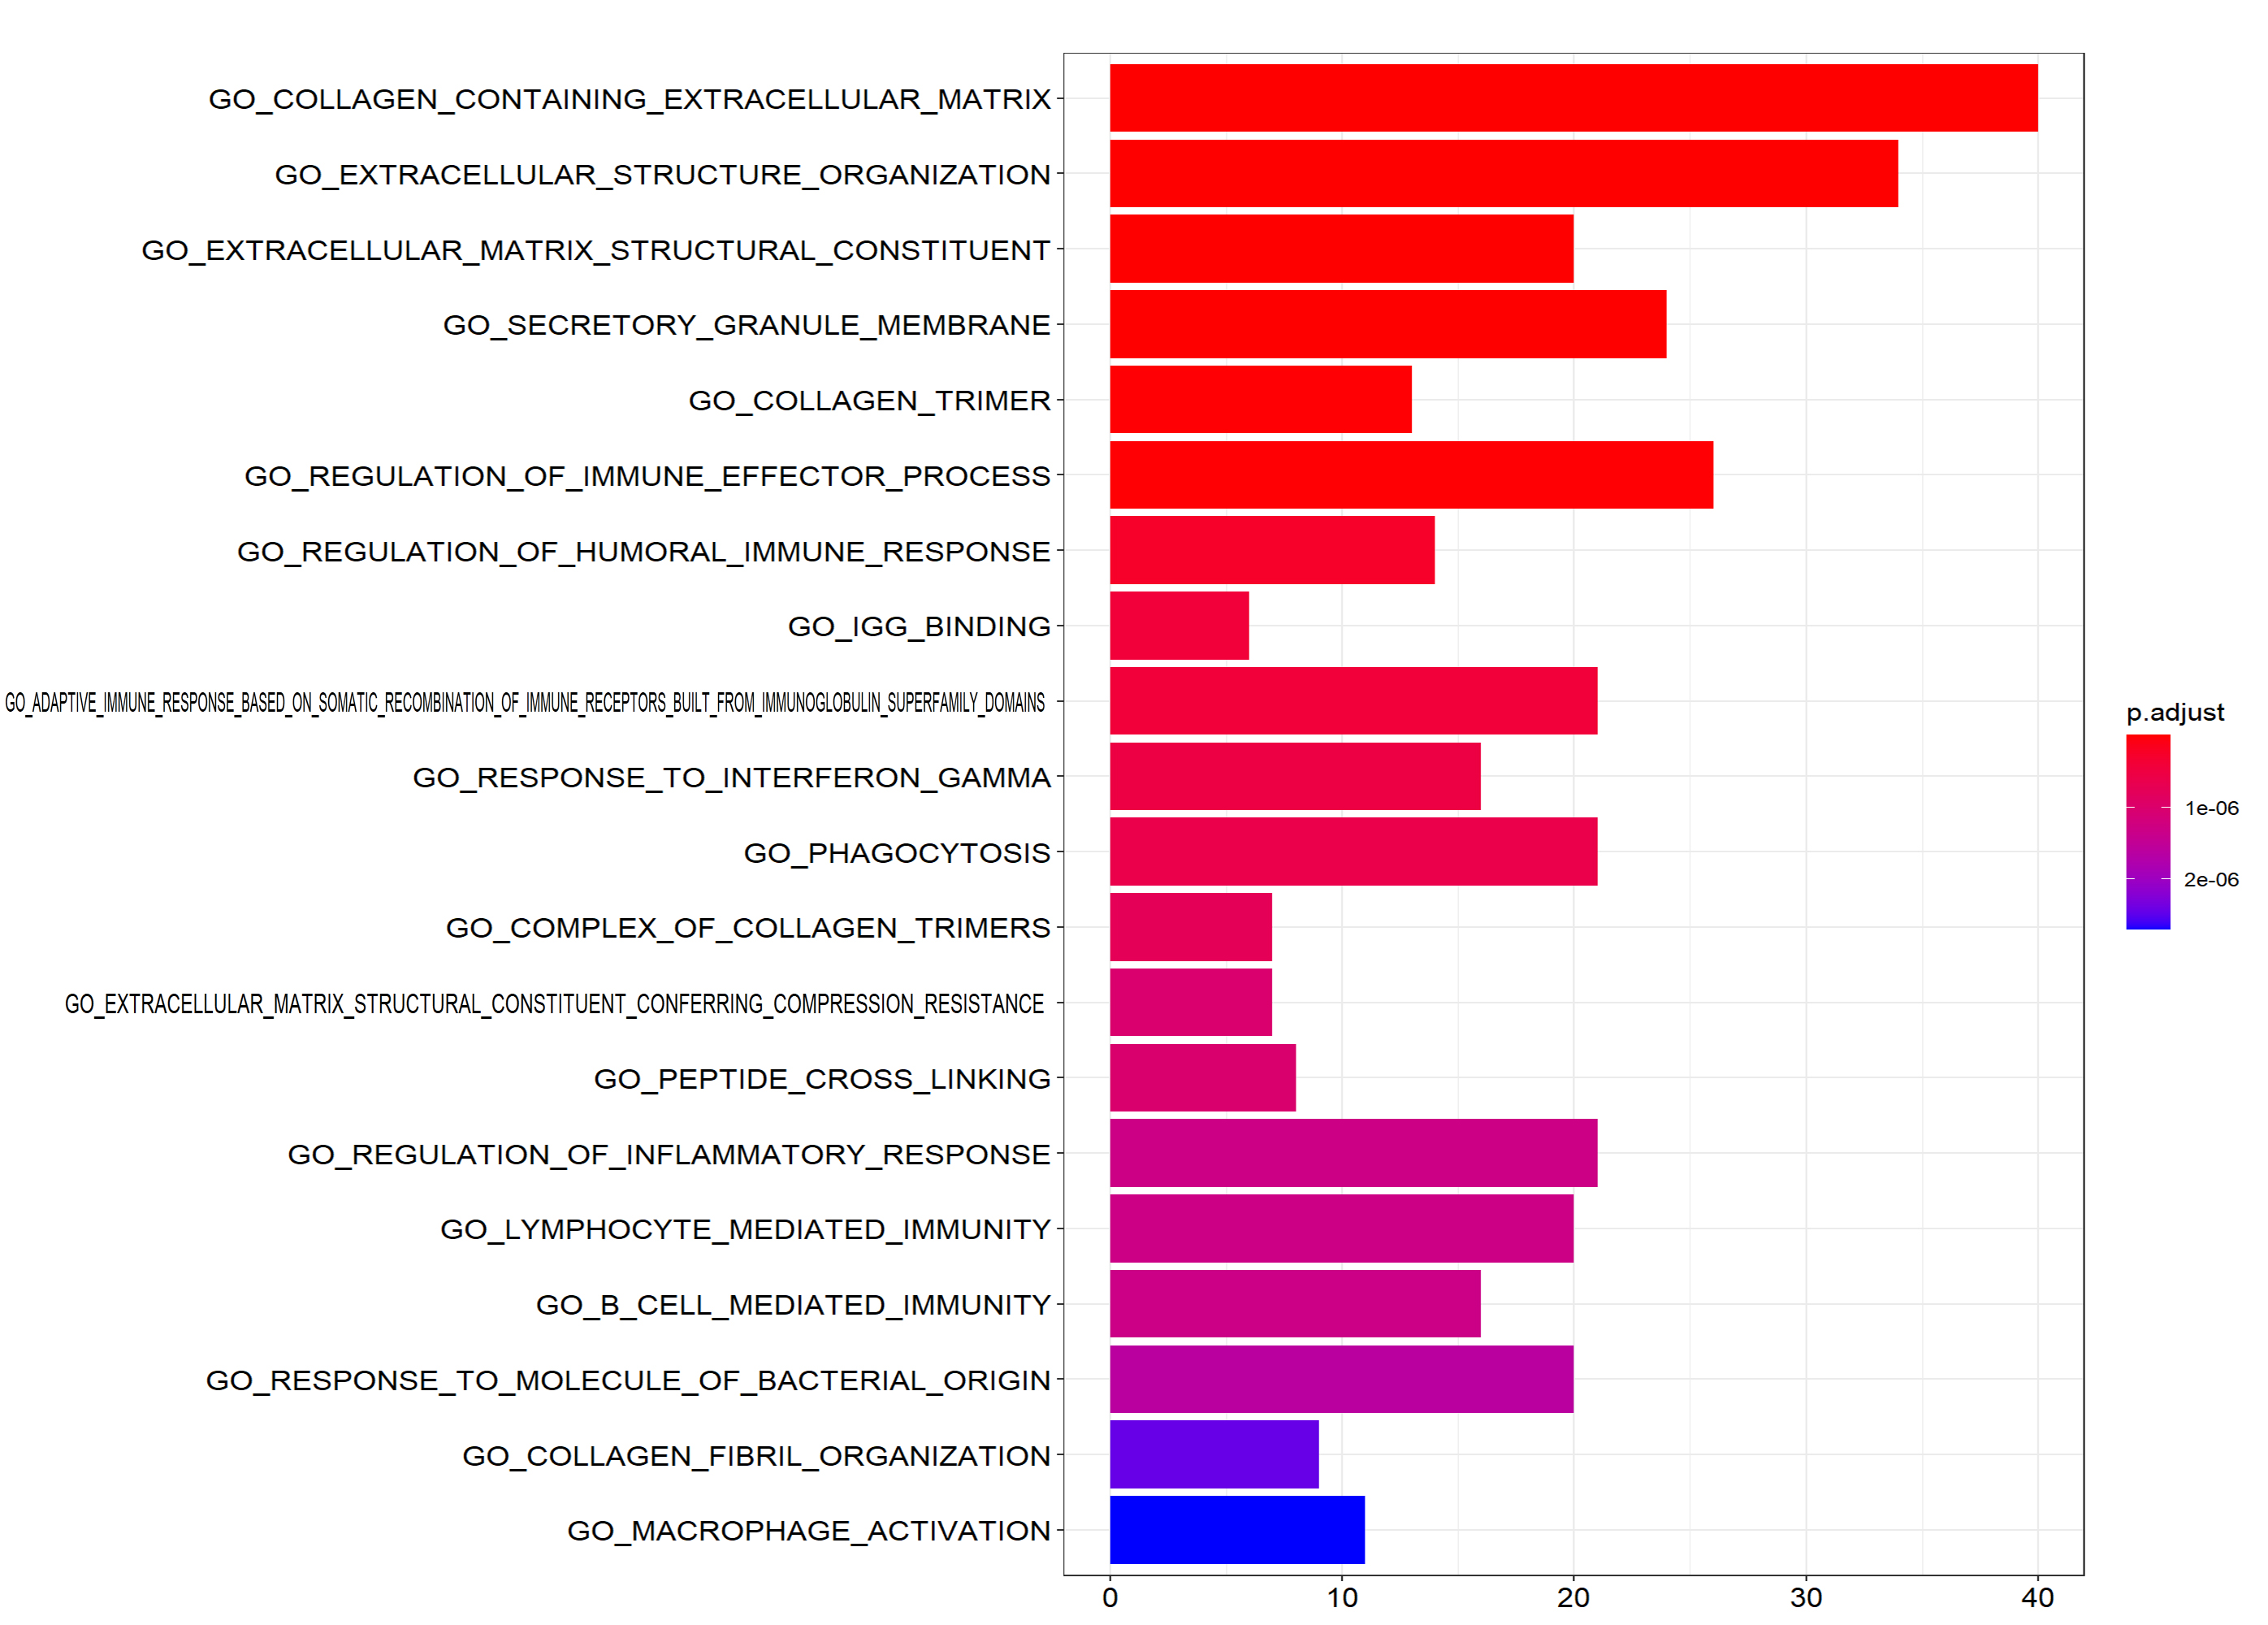
\includegraphics[width=5cm]{Figures/Path/bar-plot-s3.jpg} }}%
    \qquad
    \subfloat[\centering GSEA for S3. ]{{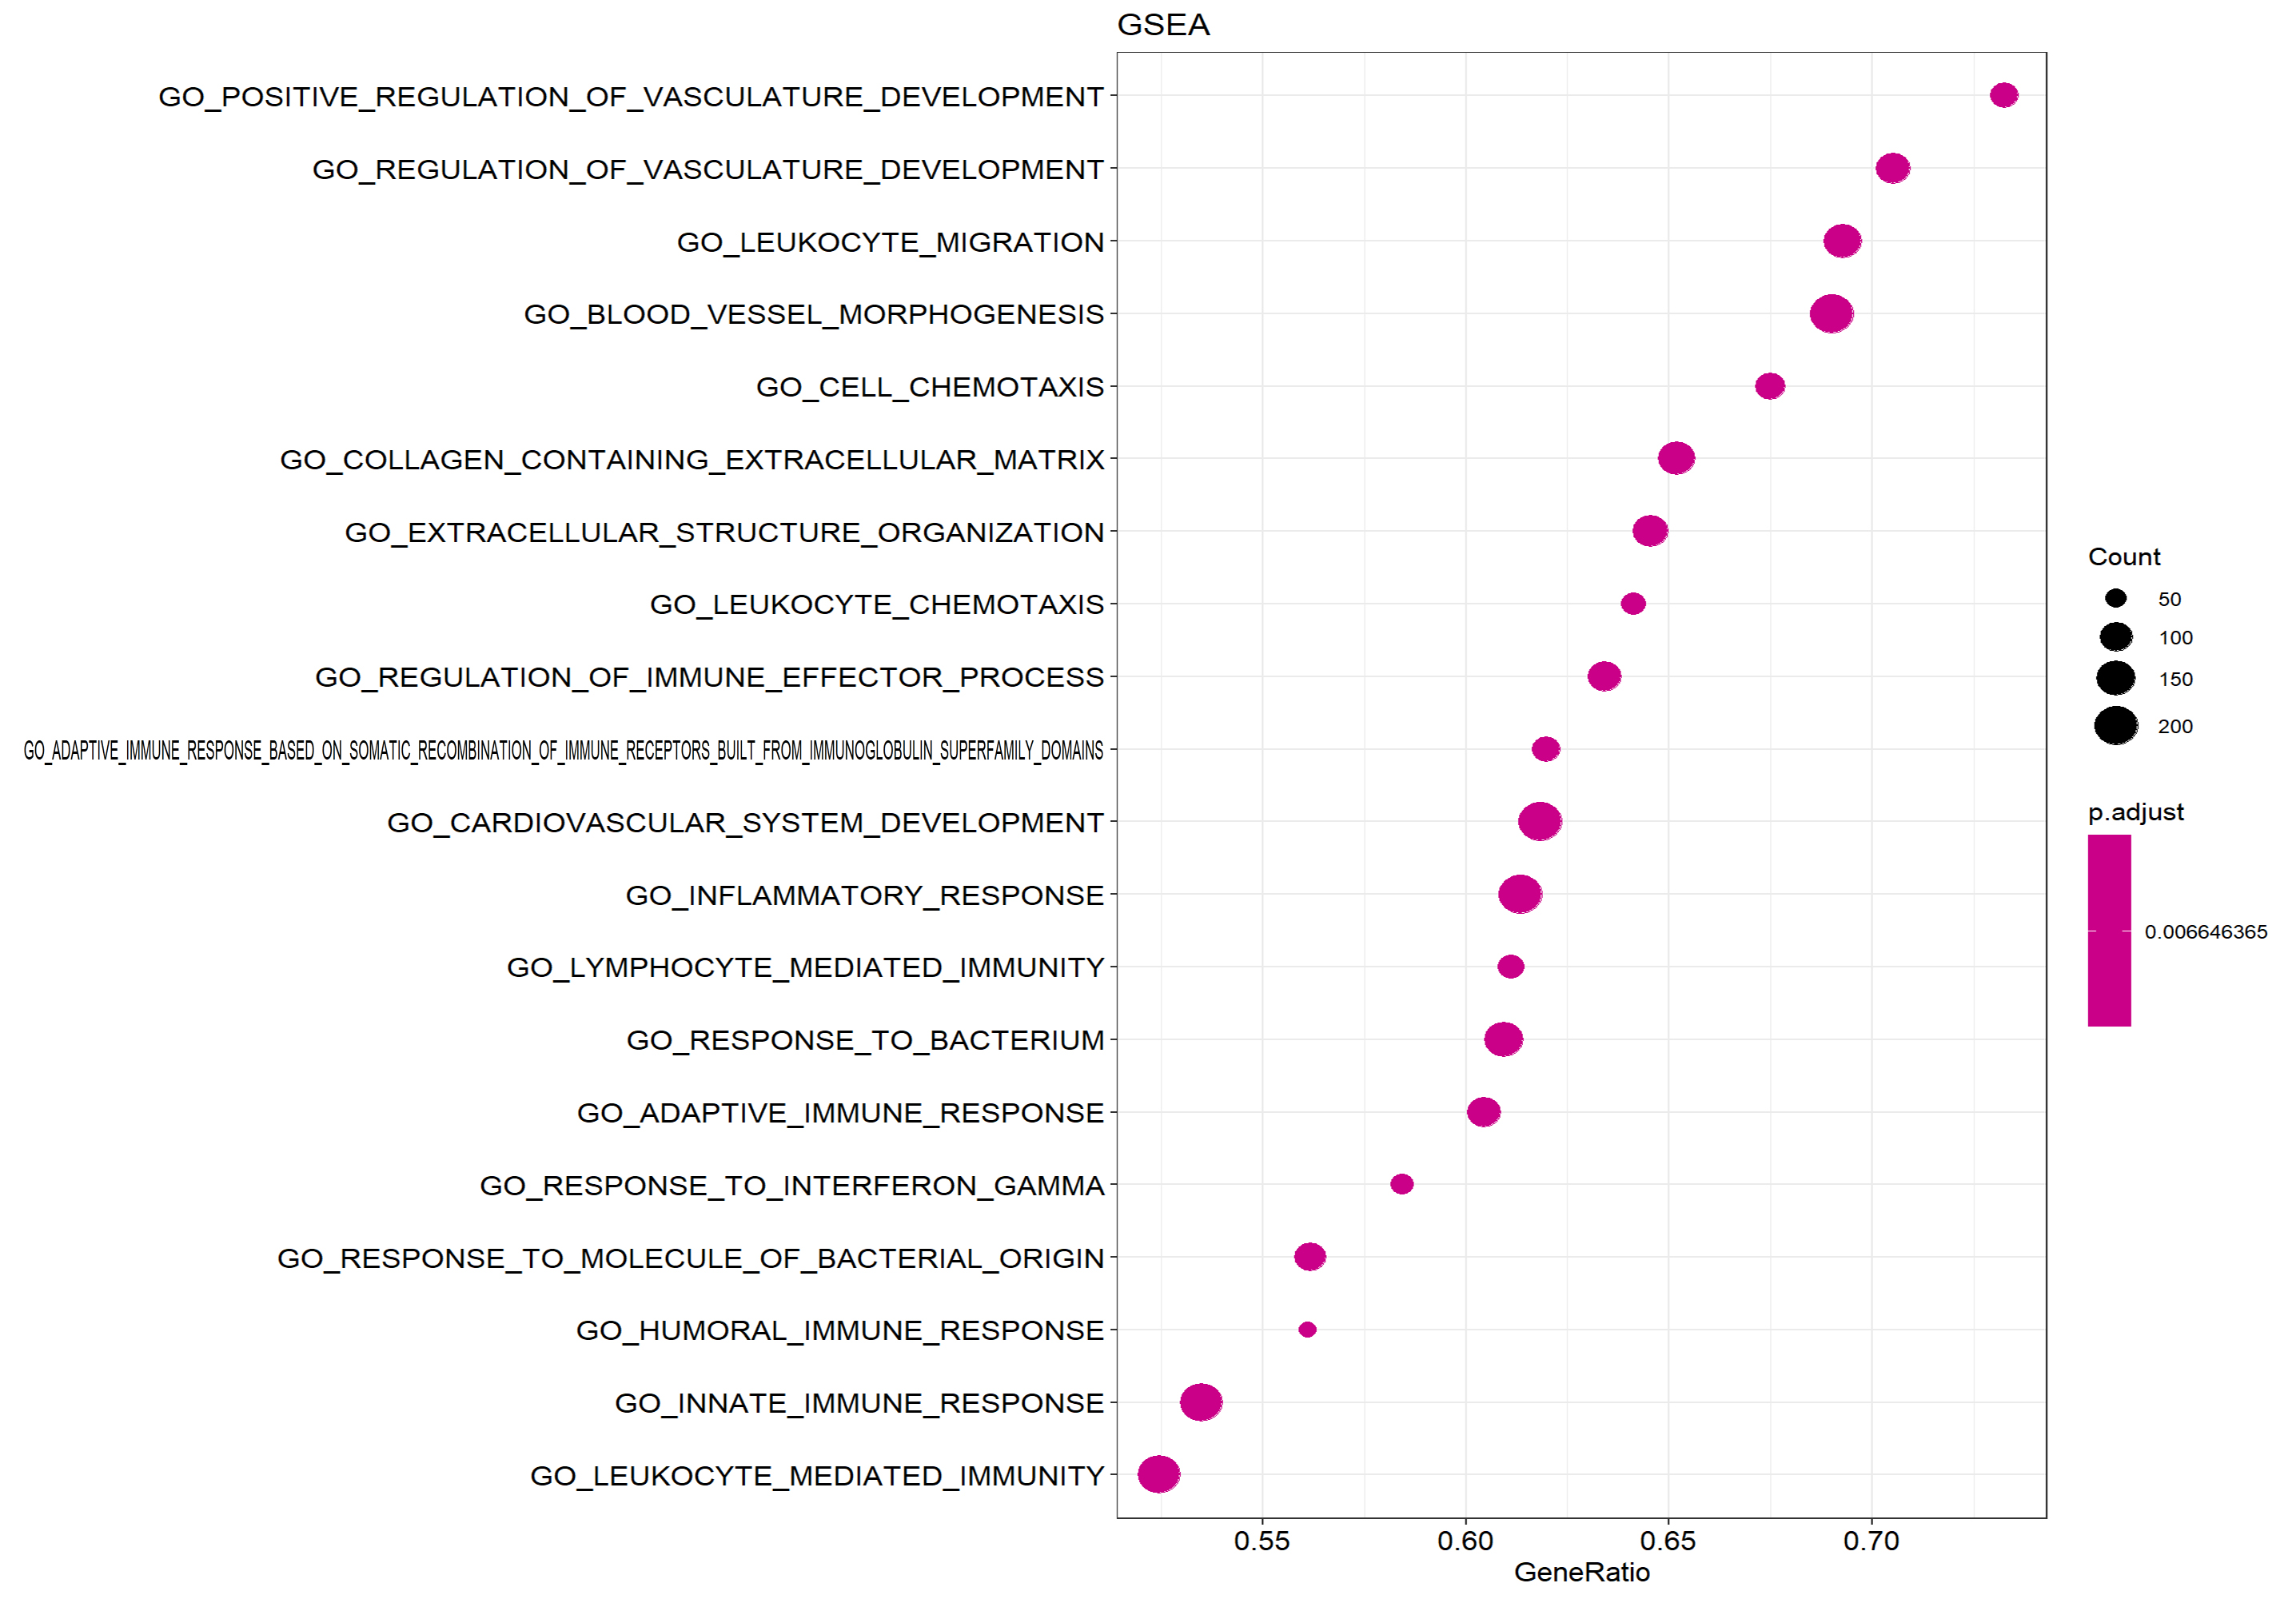
\includegraphics[width=5cm]{Figures/Path/dot-plot-s3.jpg} }}%
\caption{Bar plot and dot plot visualization for over representation analysis and gene set enrichment analysis, respectively, of sutbype in PCx-PD.}
\label{fig:path-pd-sub}%
\end{figure}

\textbf{PCx-HD.} Briefly, the associated pathways of ORA were immune system and inflammatory processes, extracellular matrix and granules. On the other hand, the related pathways of GSEA in this datasets were about cellular respiration (ATP, NADH), cytosolic ribosome, and protein localization. The resulted pathways linked with brain were node of Ranvier, tau protein binding, substantia nigra development, and main axon.

\begin{figure}[!ht]%
    \centering
    \subfloat{{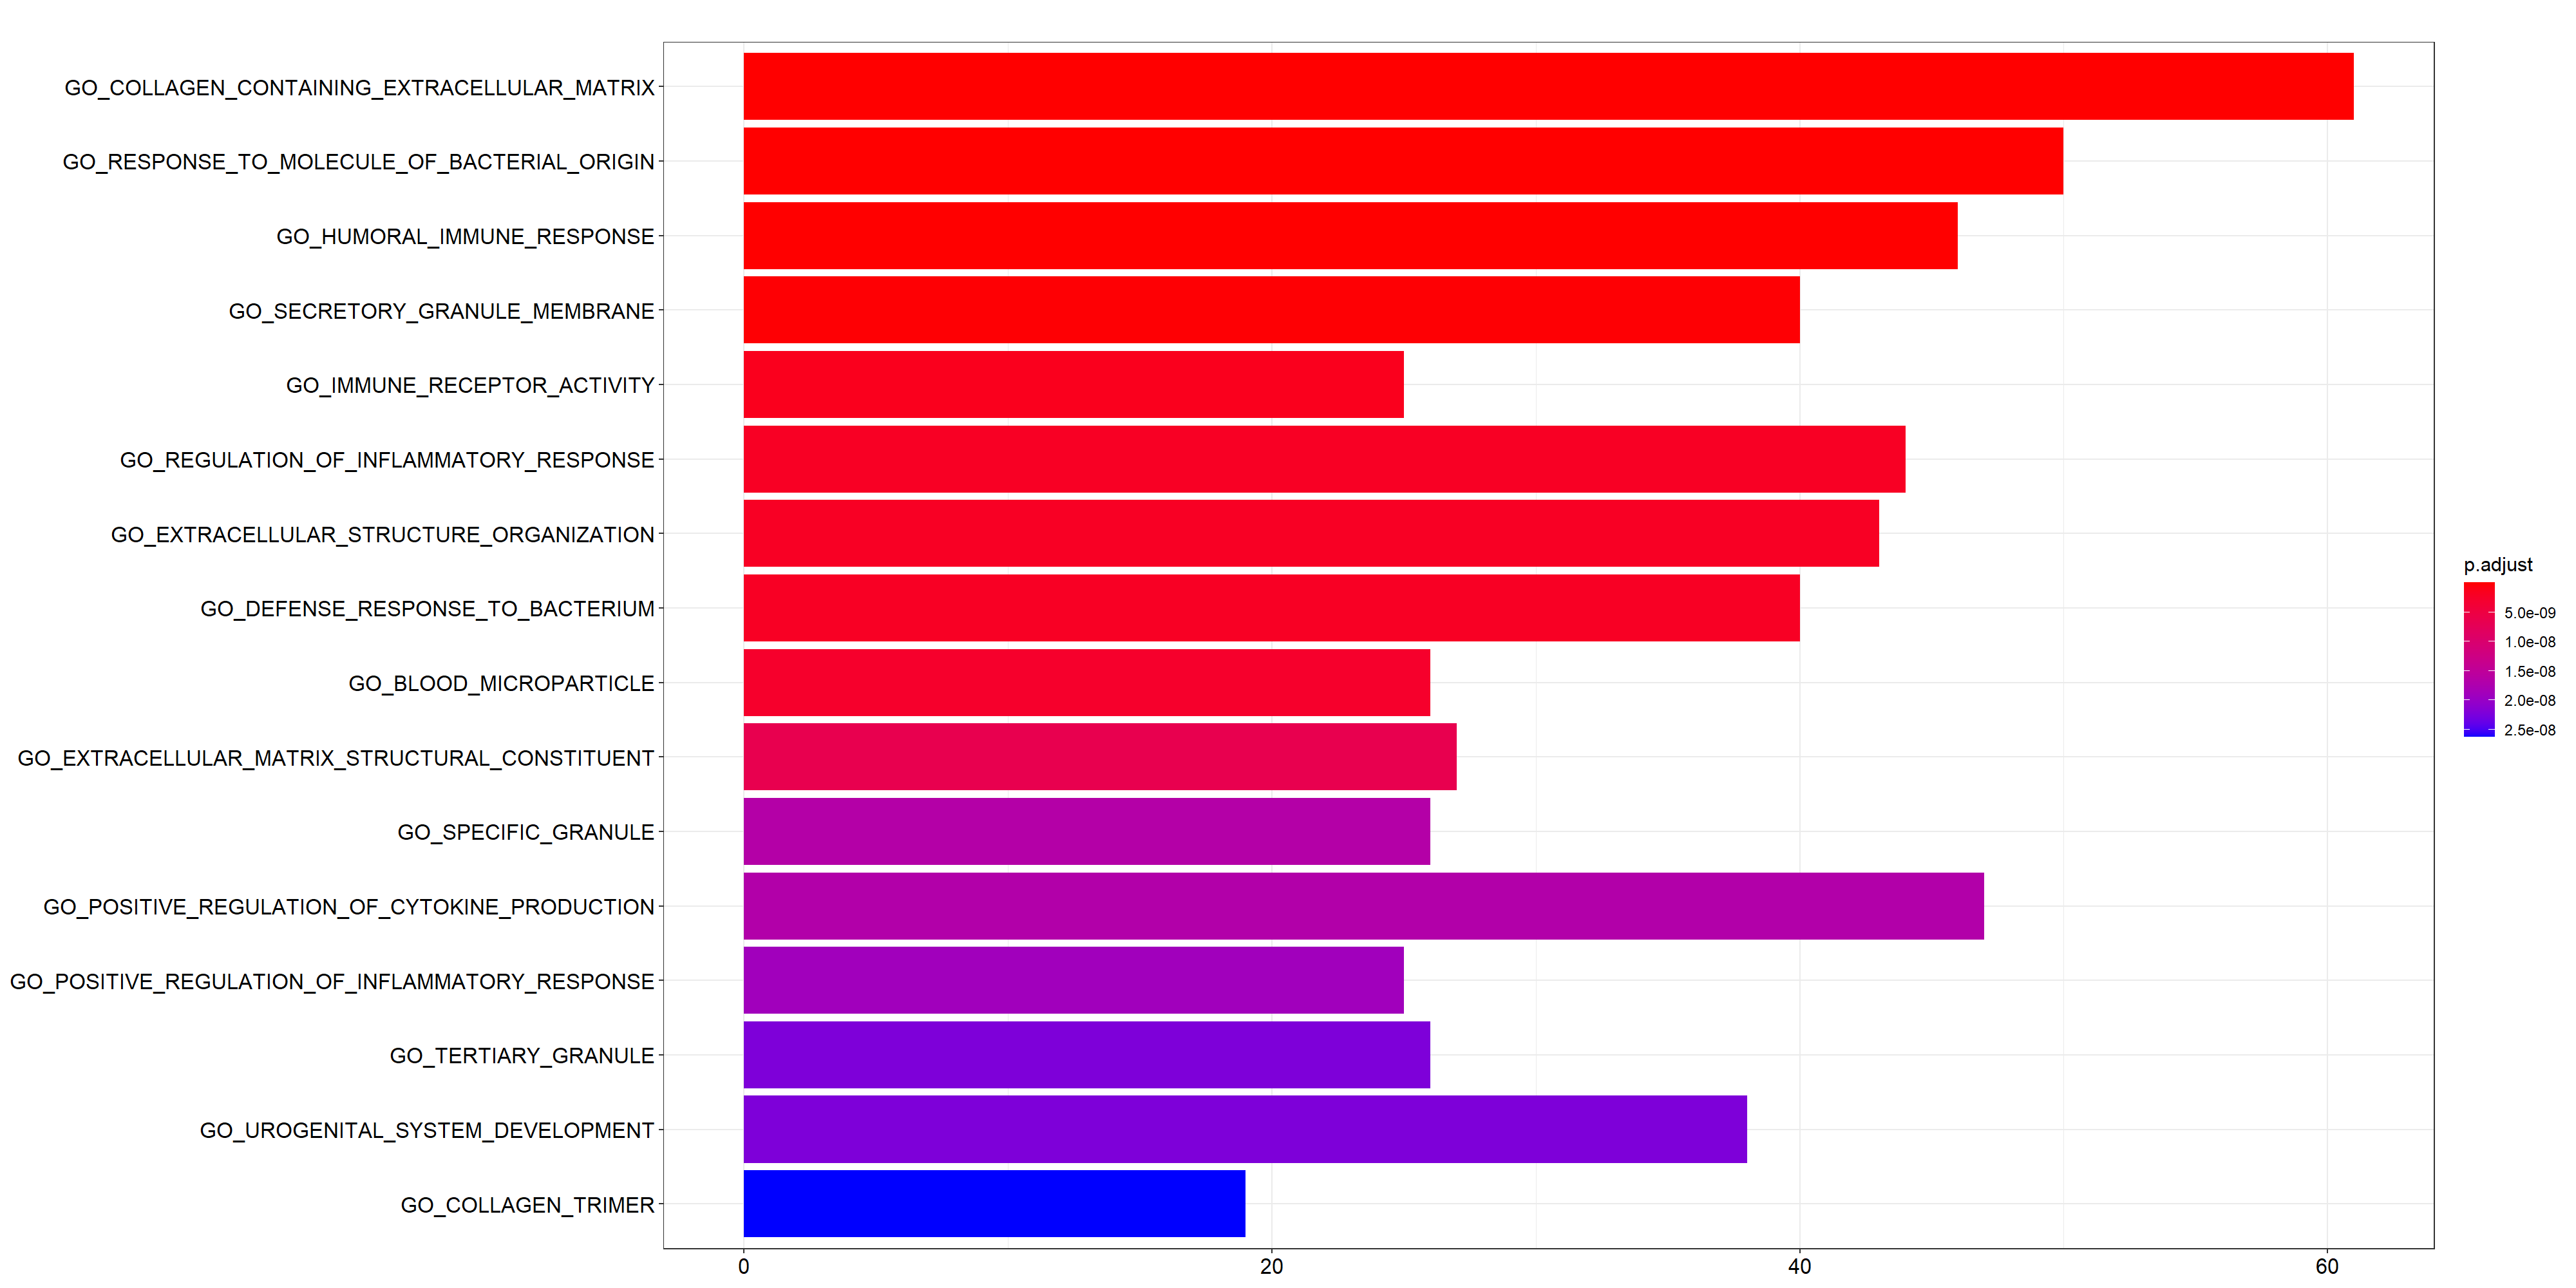
\includegraphics[width=9cm]{Figures/Path/CTLvsHD_barplot.png} }}%
    \\
    \subfloat{{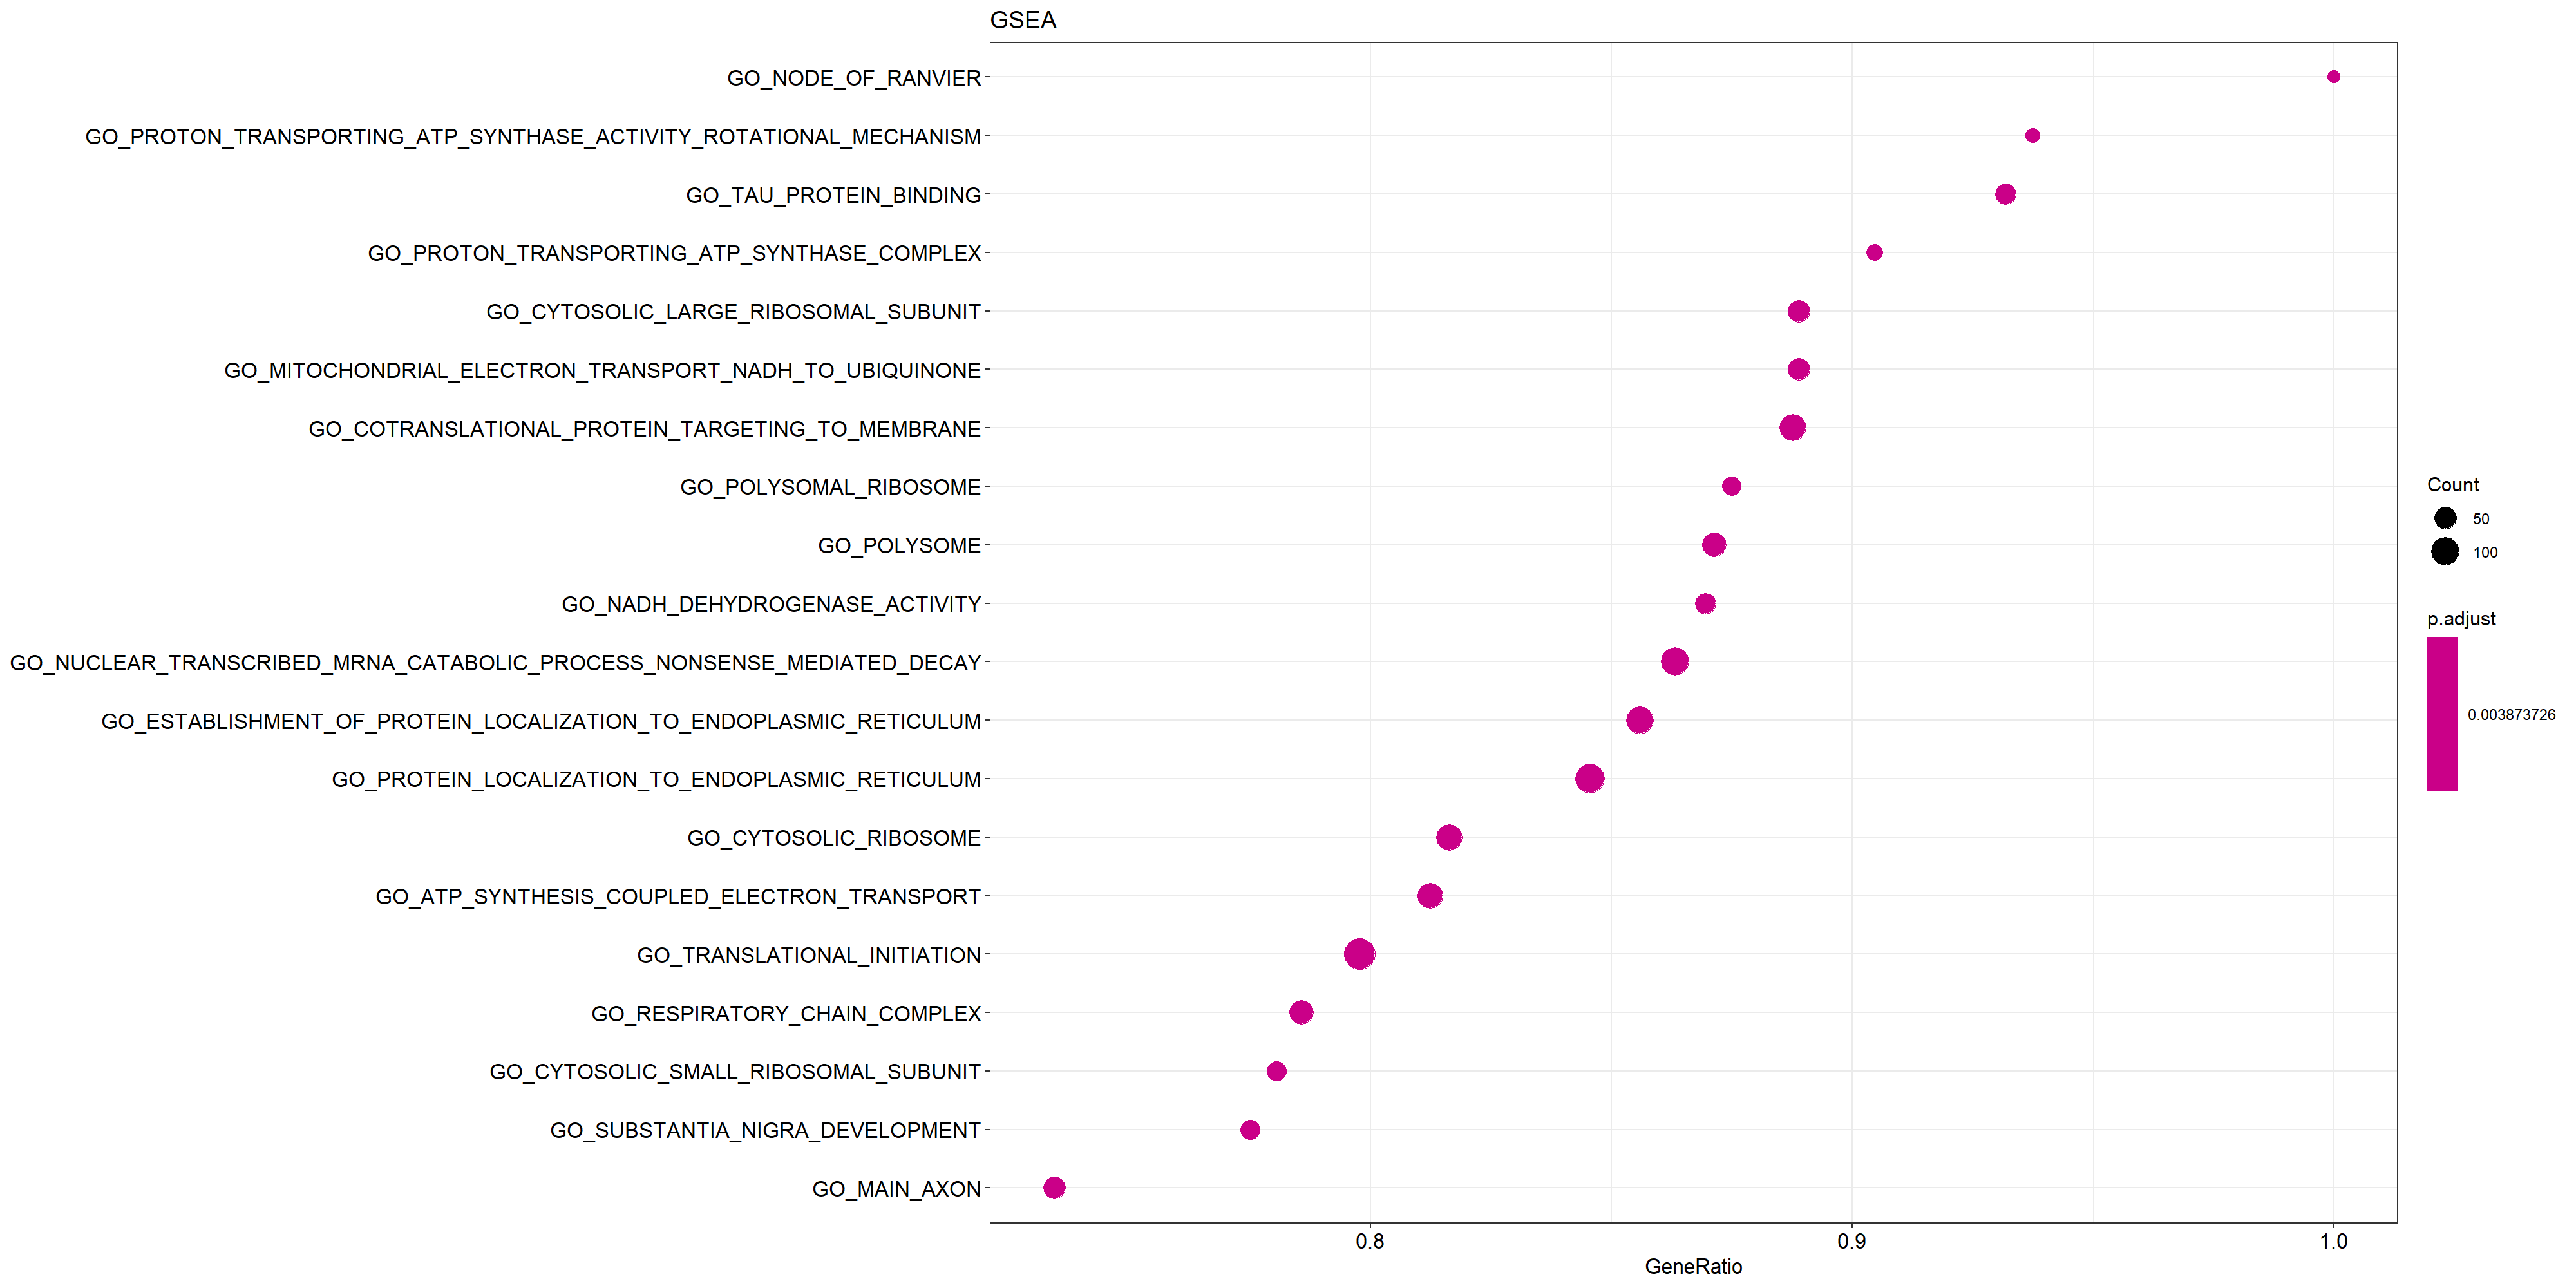
\includegraphics[width=9cm]{Figures/Path/CTLvsHD_dotplot.png} }}%
\caption{Bar plot and dot plot visualization for over representation analysis and gene set enrichment analysis, respectively, of PCx-HD.}
\label{fig:path-pcx-hd}%
\end{figure}

\textbf{Blood-HD.} Interestingly, although the male and female set did not share any common DEG, they do have in common seven out of 20 pathways of GSEA (see Fig. \ref{fig:path-blood-hd}). The distinct pathways in female are superoxide anion generation, regulation of phagocytosis, and response to interlukein 12, whereas the male pathways relate with granule and membrane raft organization. However, in the ORA results, one pathway is shared among sexes: regulation of chromosome organization. The female set contains routes related to RNA, while the male set comprises paths associated with chromatin and telomeres. It is relevant to highlight that the ORA results for the male part obtained an adjusted p-value of 0.47. 

\begin{figure}[!ht]%
    \centering
    \subfloat{{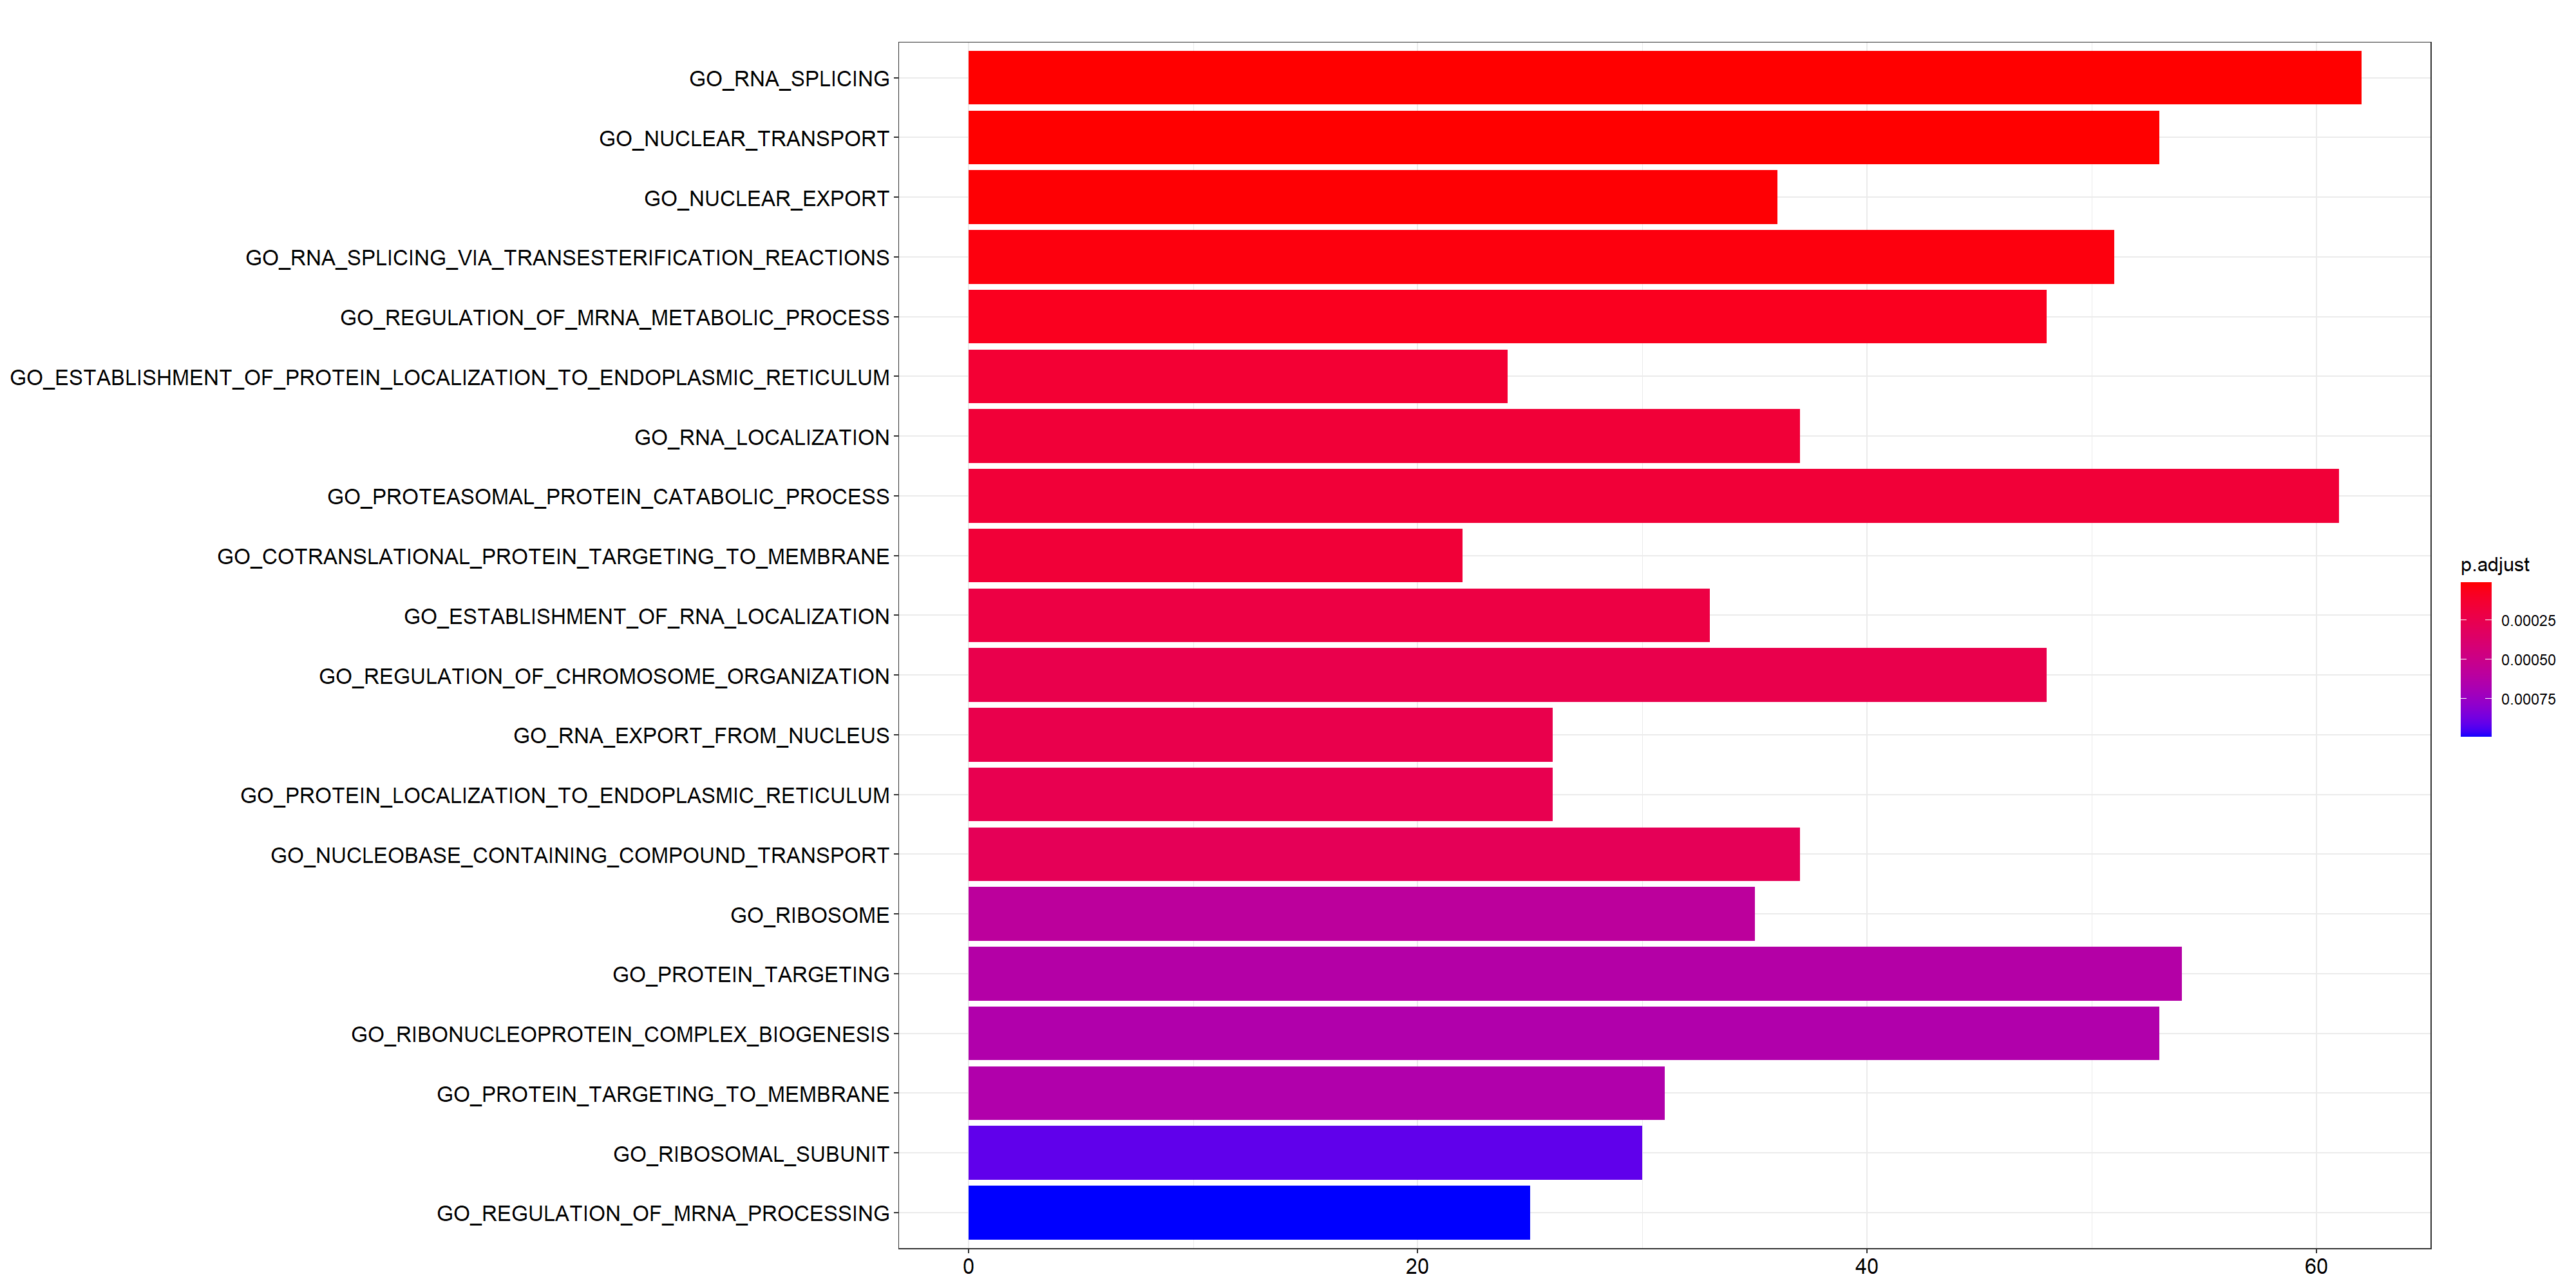
\includegraphics[width=5cm]{Figures/Path/CTLvsHD_ef_barplot.png} }}%
    \qquad
    \subfloat{{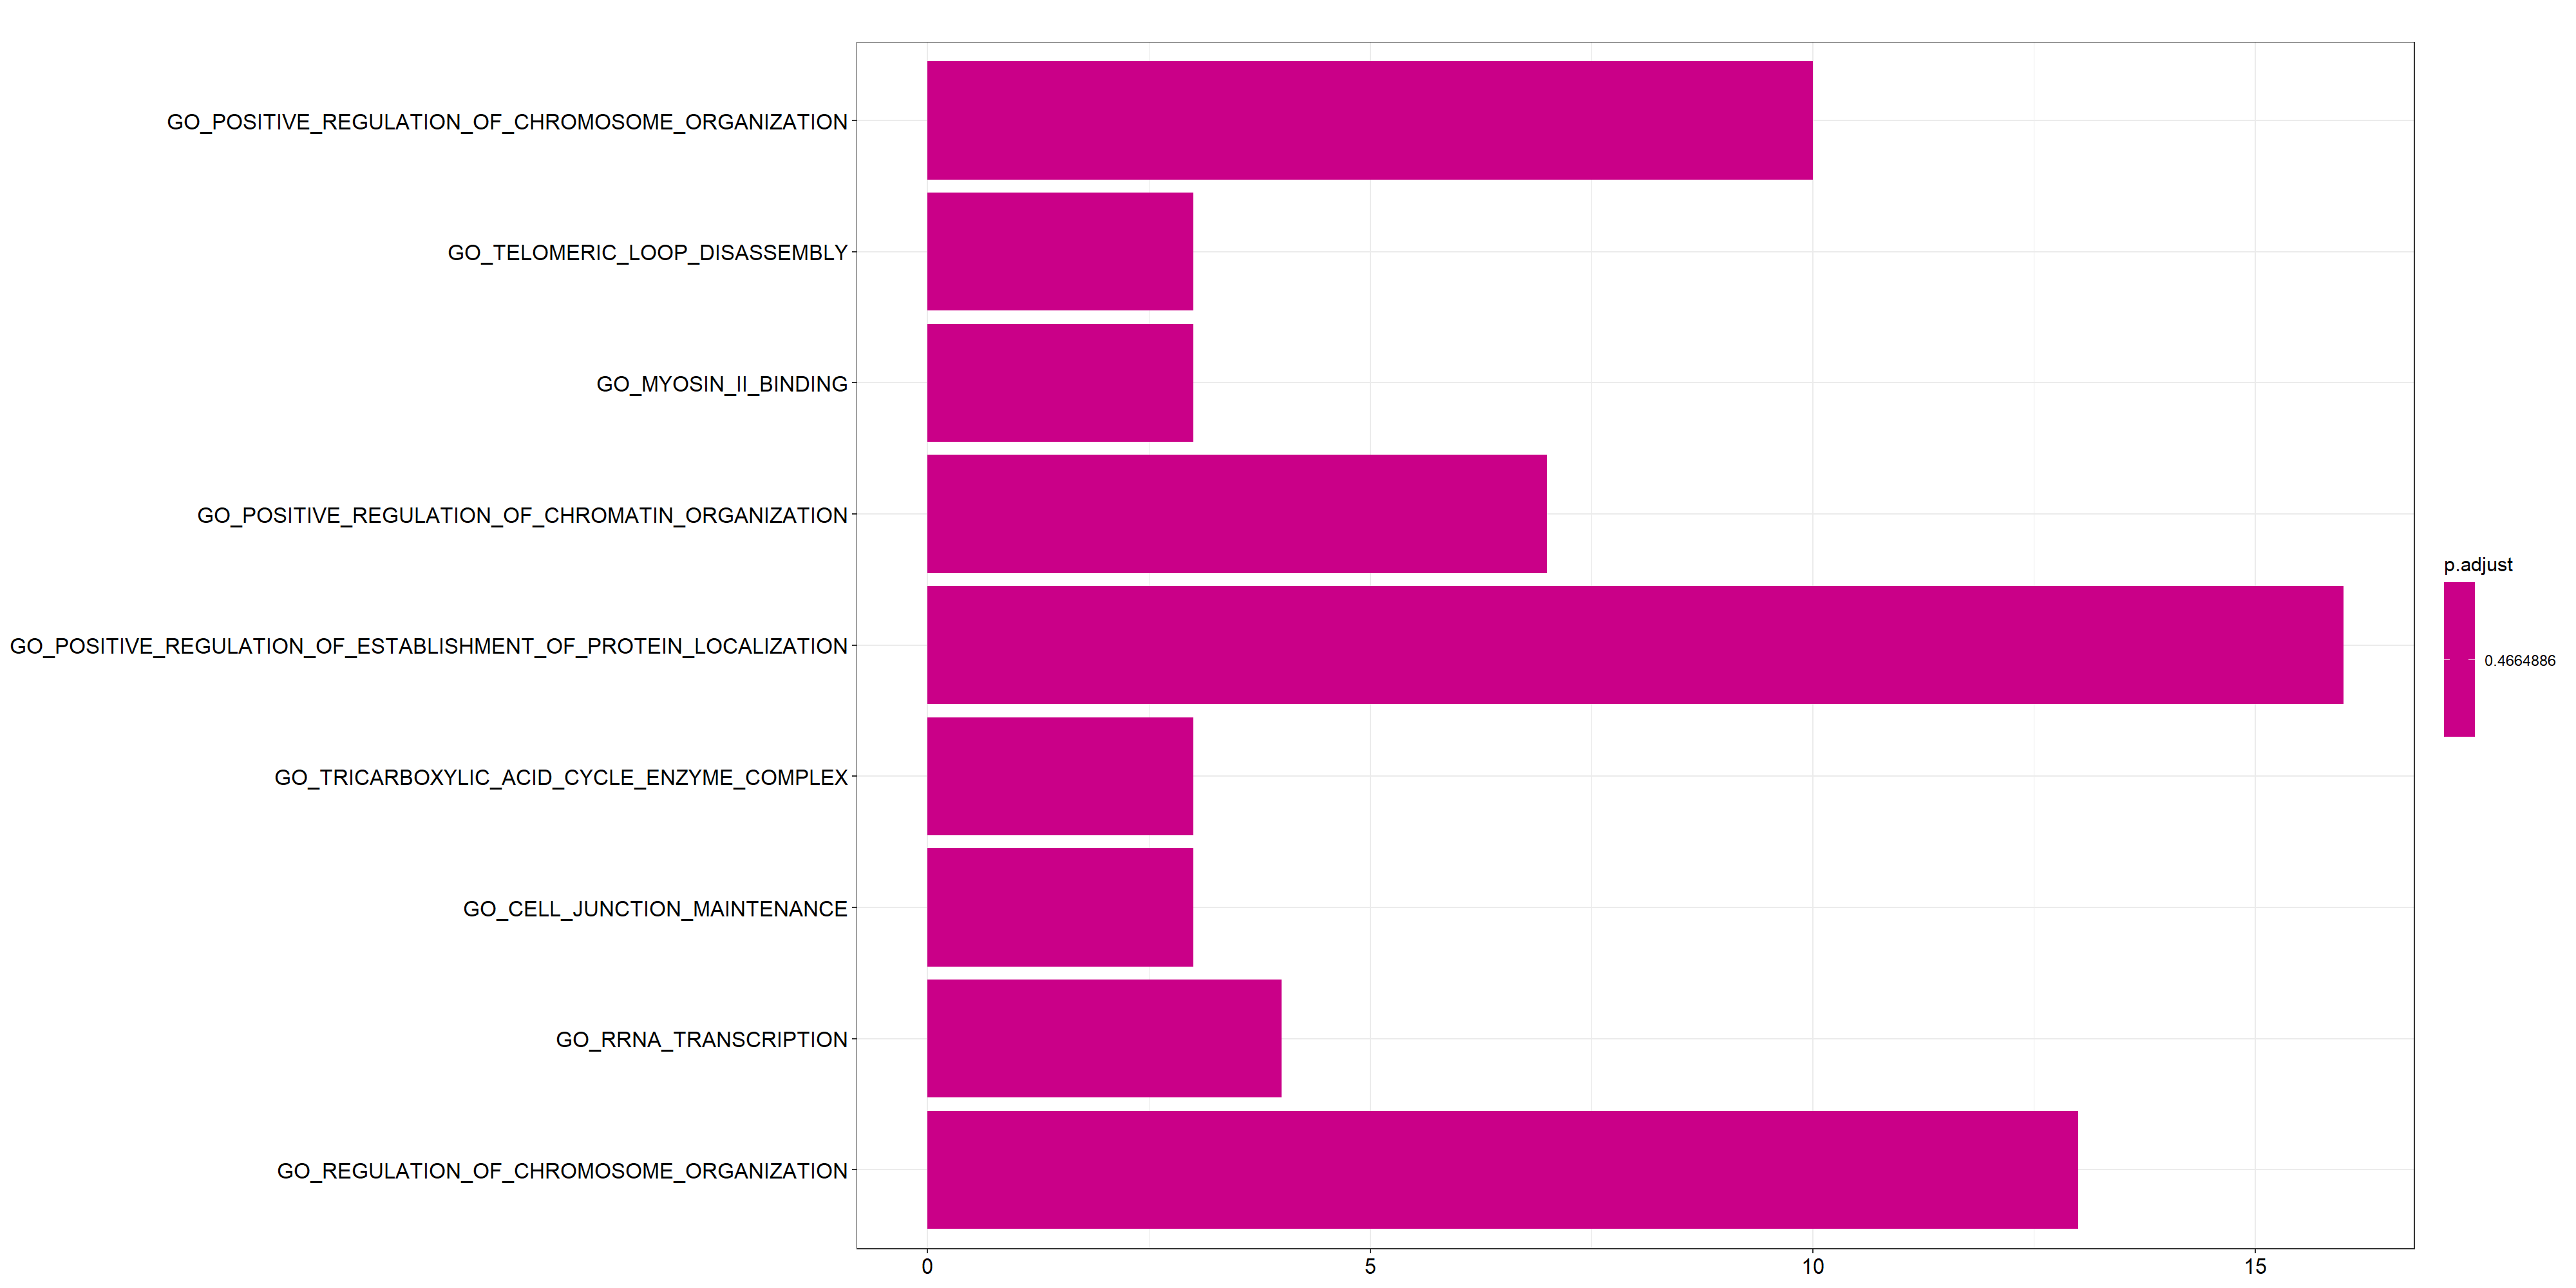
\includegraphics[width=5cm]{Figures/Path/CTLvsHD_em_barplot.png} }}%
    \\
    \subfloat{{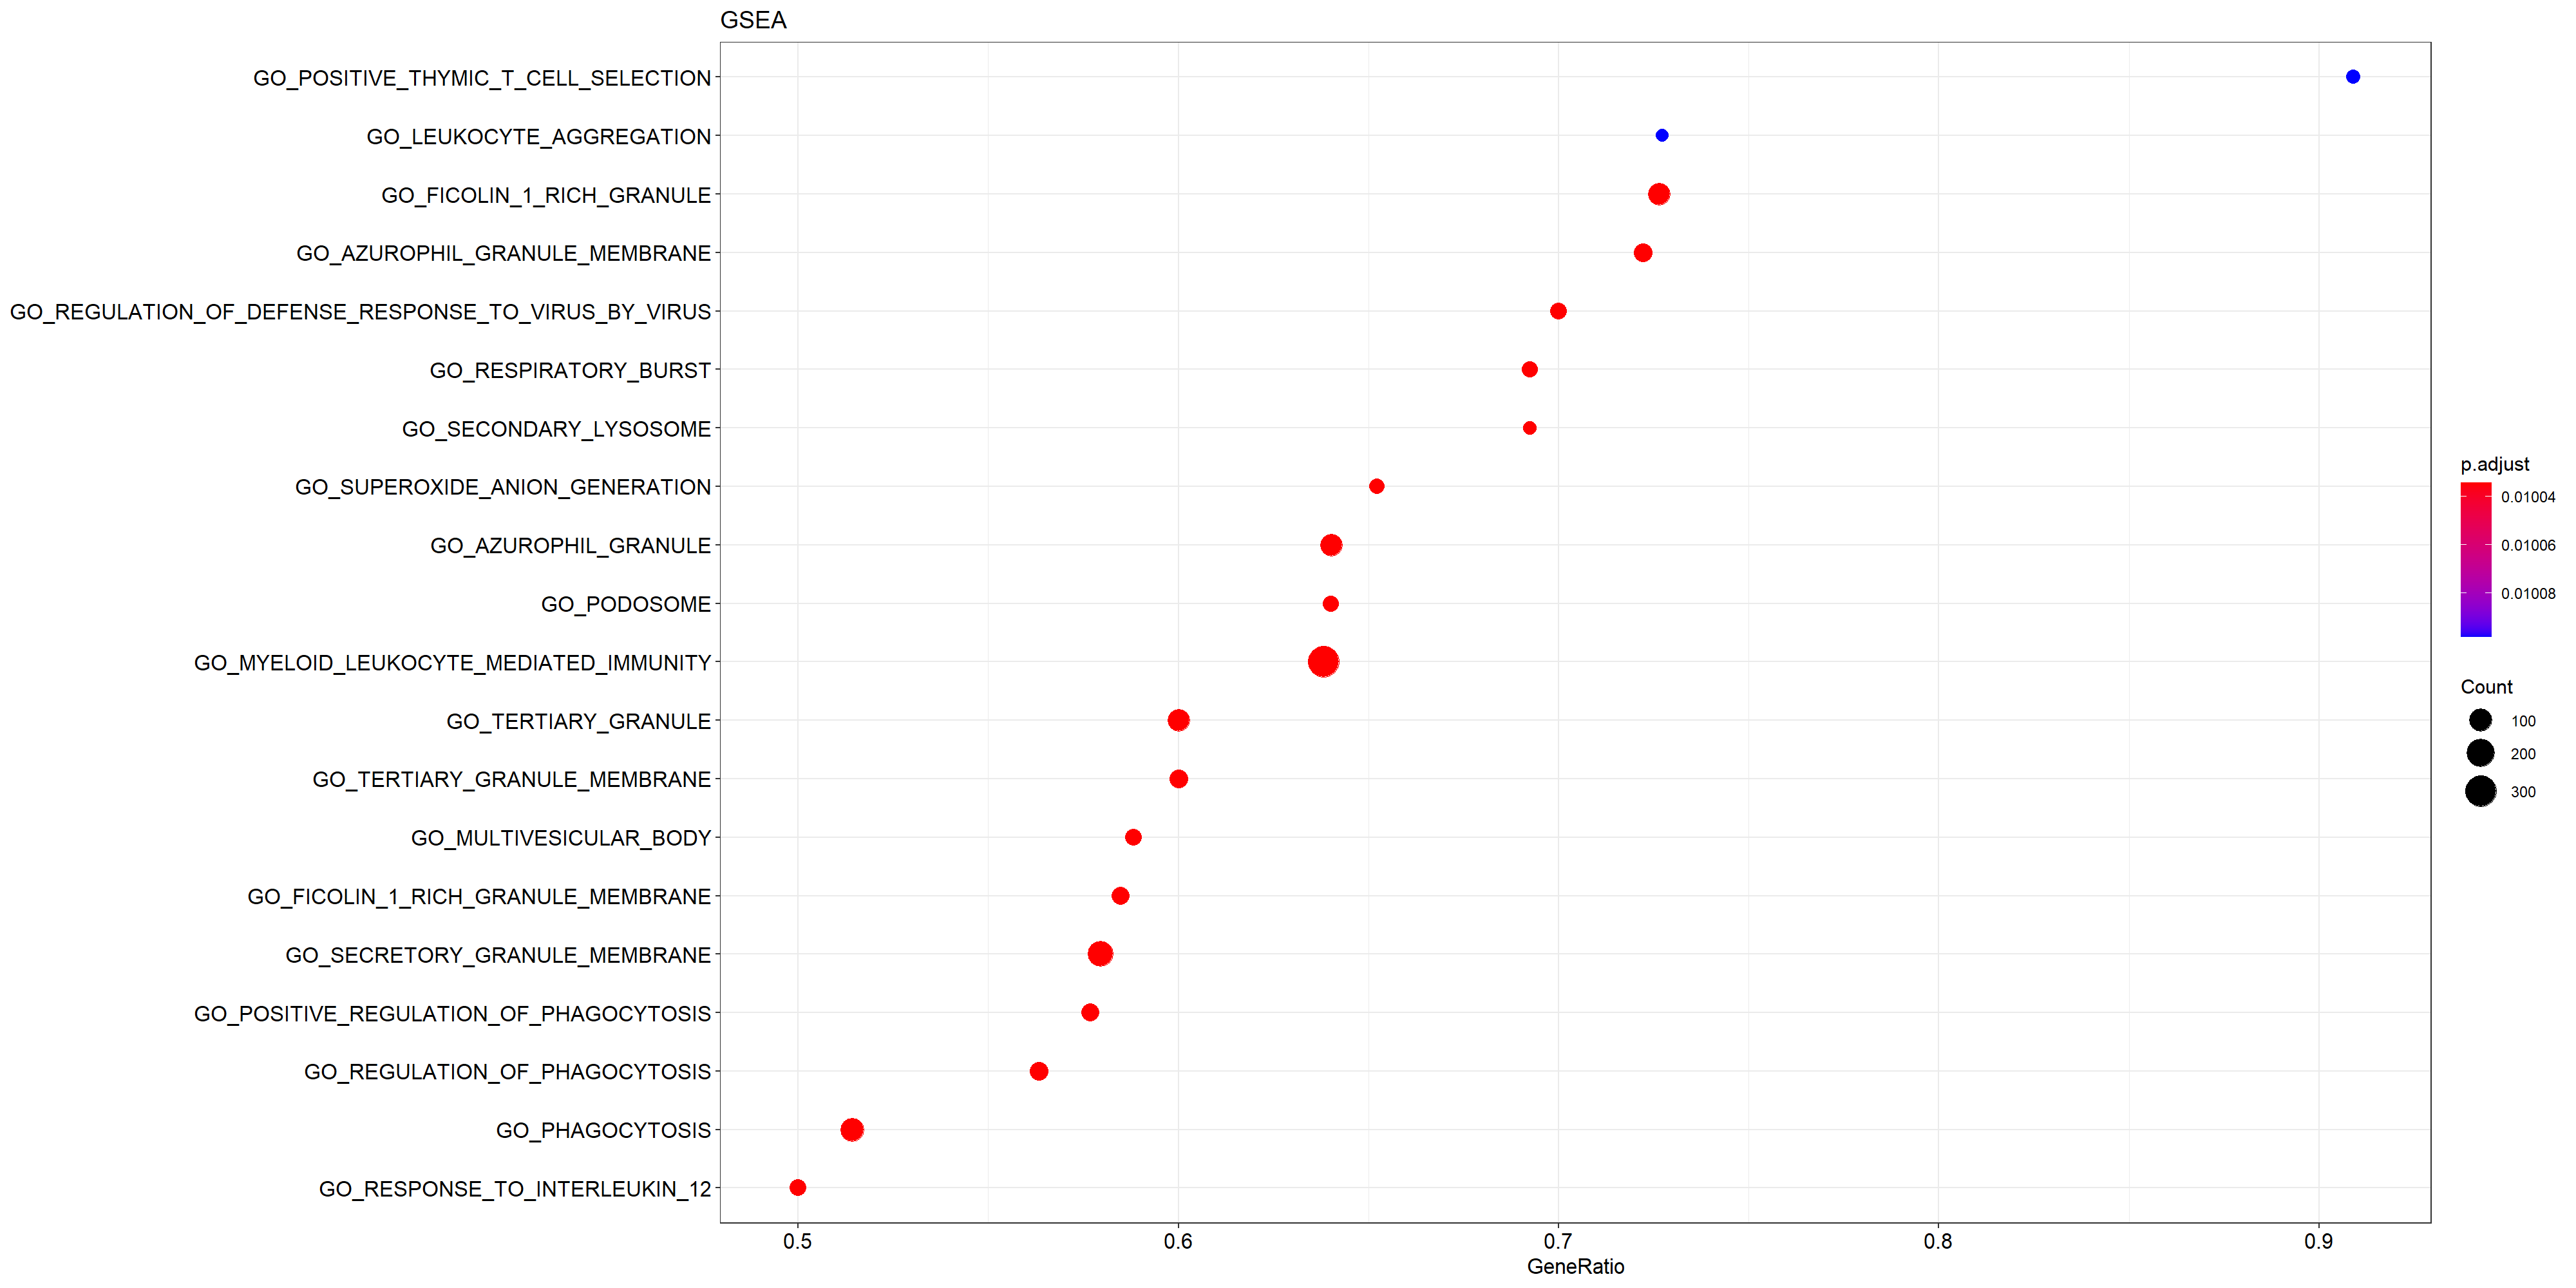
\includegraphics[width=5cm]{Figures/Path/CTLvsHD_ef_dotplot.png} }}%
    \qquad
    \subfloat{{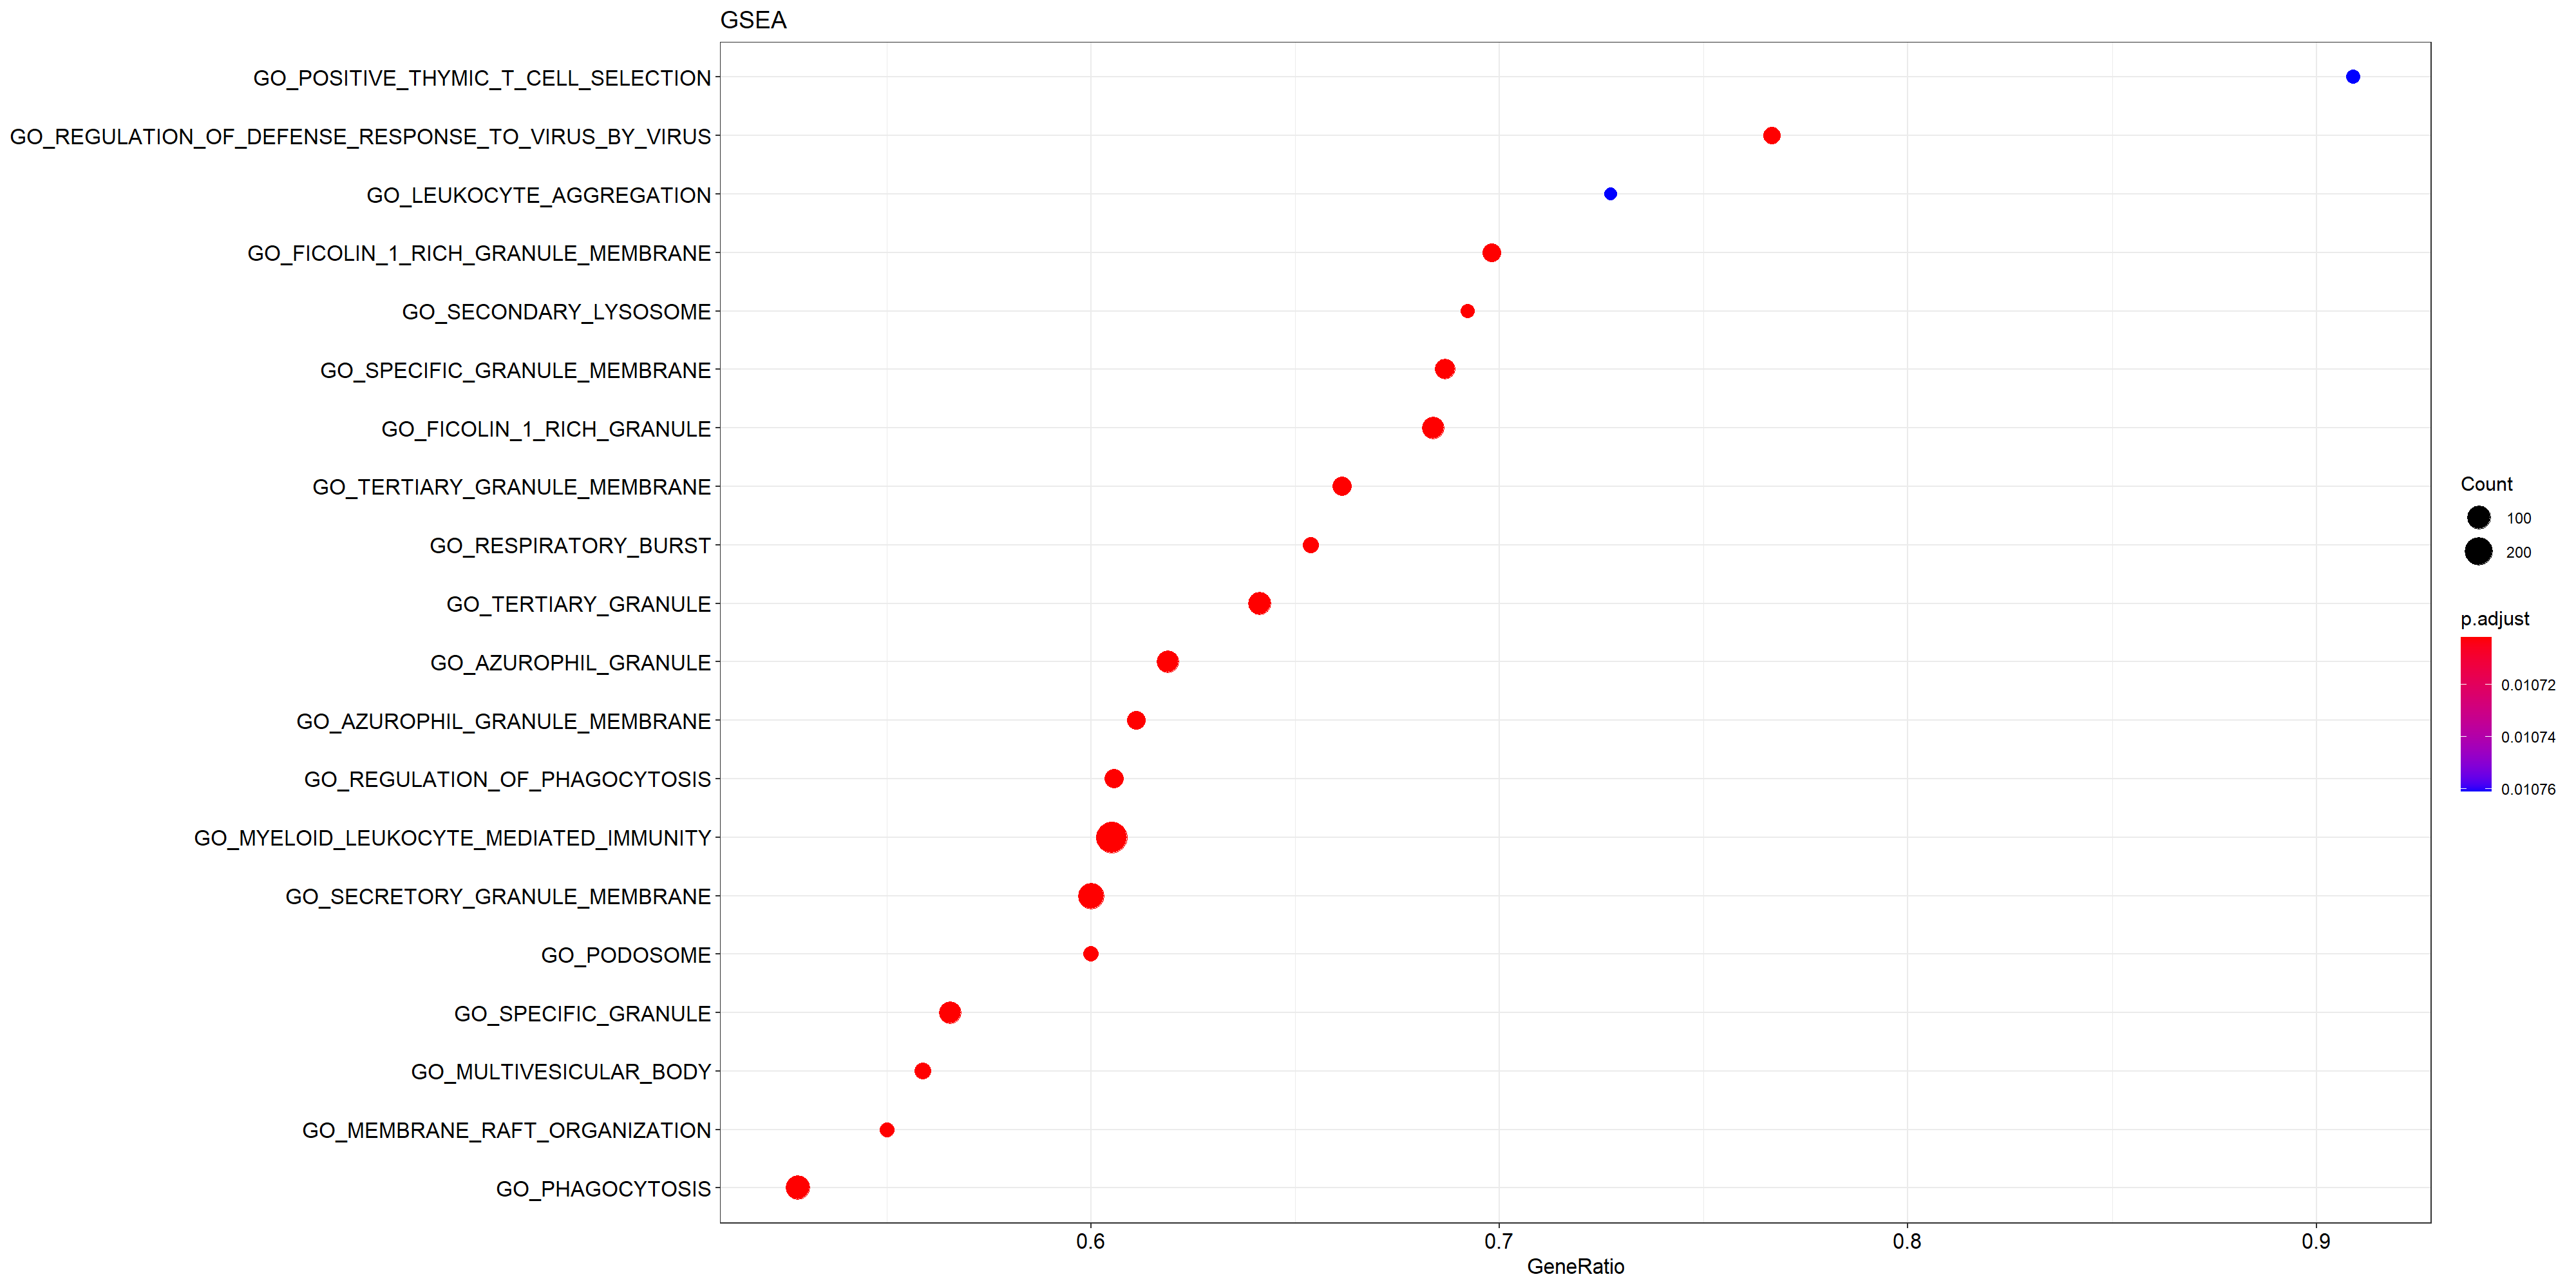
\includegraphics[width=5cm]{Figures/Path/CTLvsHD_em_dotplot.png} }}%
\caption{Bar plot and dot plot visualization for over representation analysis and gene set enrichment analysis, respectively, of Blood-HD.}
\footnotesize Left for female; right for male.
\label{fig:path-blood-hd}%
\end{figure}

The results of the female subtype functional analysis are presented in Fig. \ref{fig:path-blood-f-sub}. The ORA pathways obtained by S1 are related to mRNA processes, nuclear transport, protein localization, and ribosome. In addition, S2 has linked paths about cell killing, and proteolysis. Last, S3 has associated pathways of RNA splicing, ribosome, cell cycle, ubiquitination, and antigen-presentation. What is more, according to the dot plots, S1 is related to neuron projection guidance, membrane processes, extracellular matrix, wound healing, cell adhesion, and external stimulus response. S2 has been related to lipid metabolism, transporter activity (ions), secretory processes, leukocyte activation, reproduction, and neuron project as well. Also, S3 relates to extracelluar matrix, immune response and inflammation, adhesion, wound healing, circulatory system, and cell motility pathways.

\begin{figure}[!ht]%
    \centering
    \subfloat[\centering ORA for S1. ]{{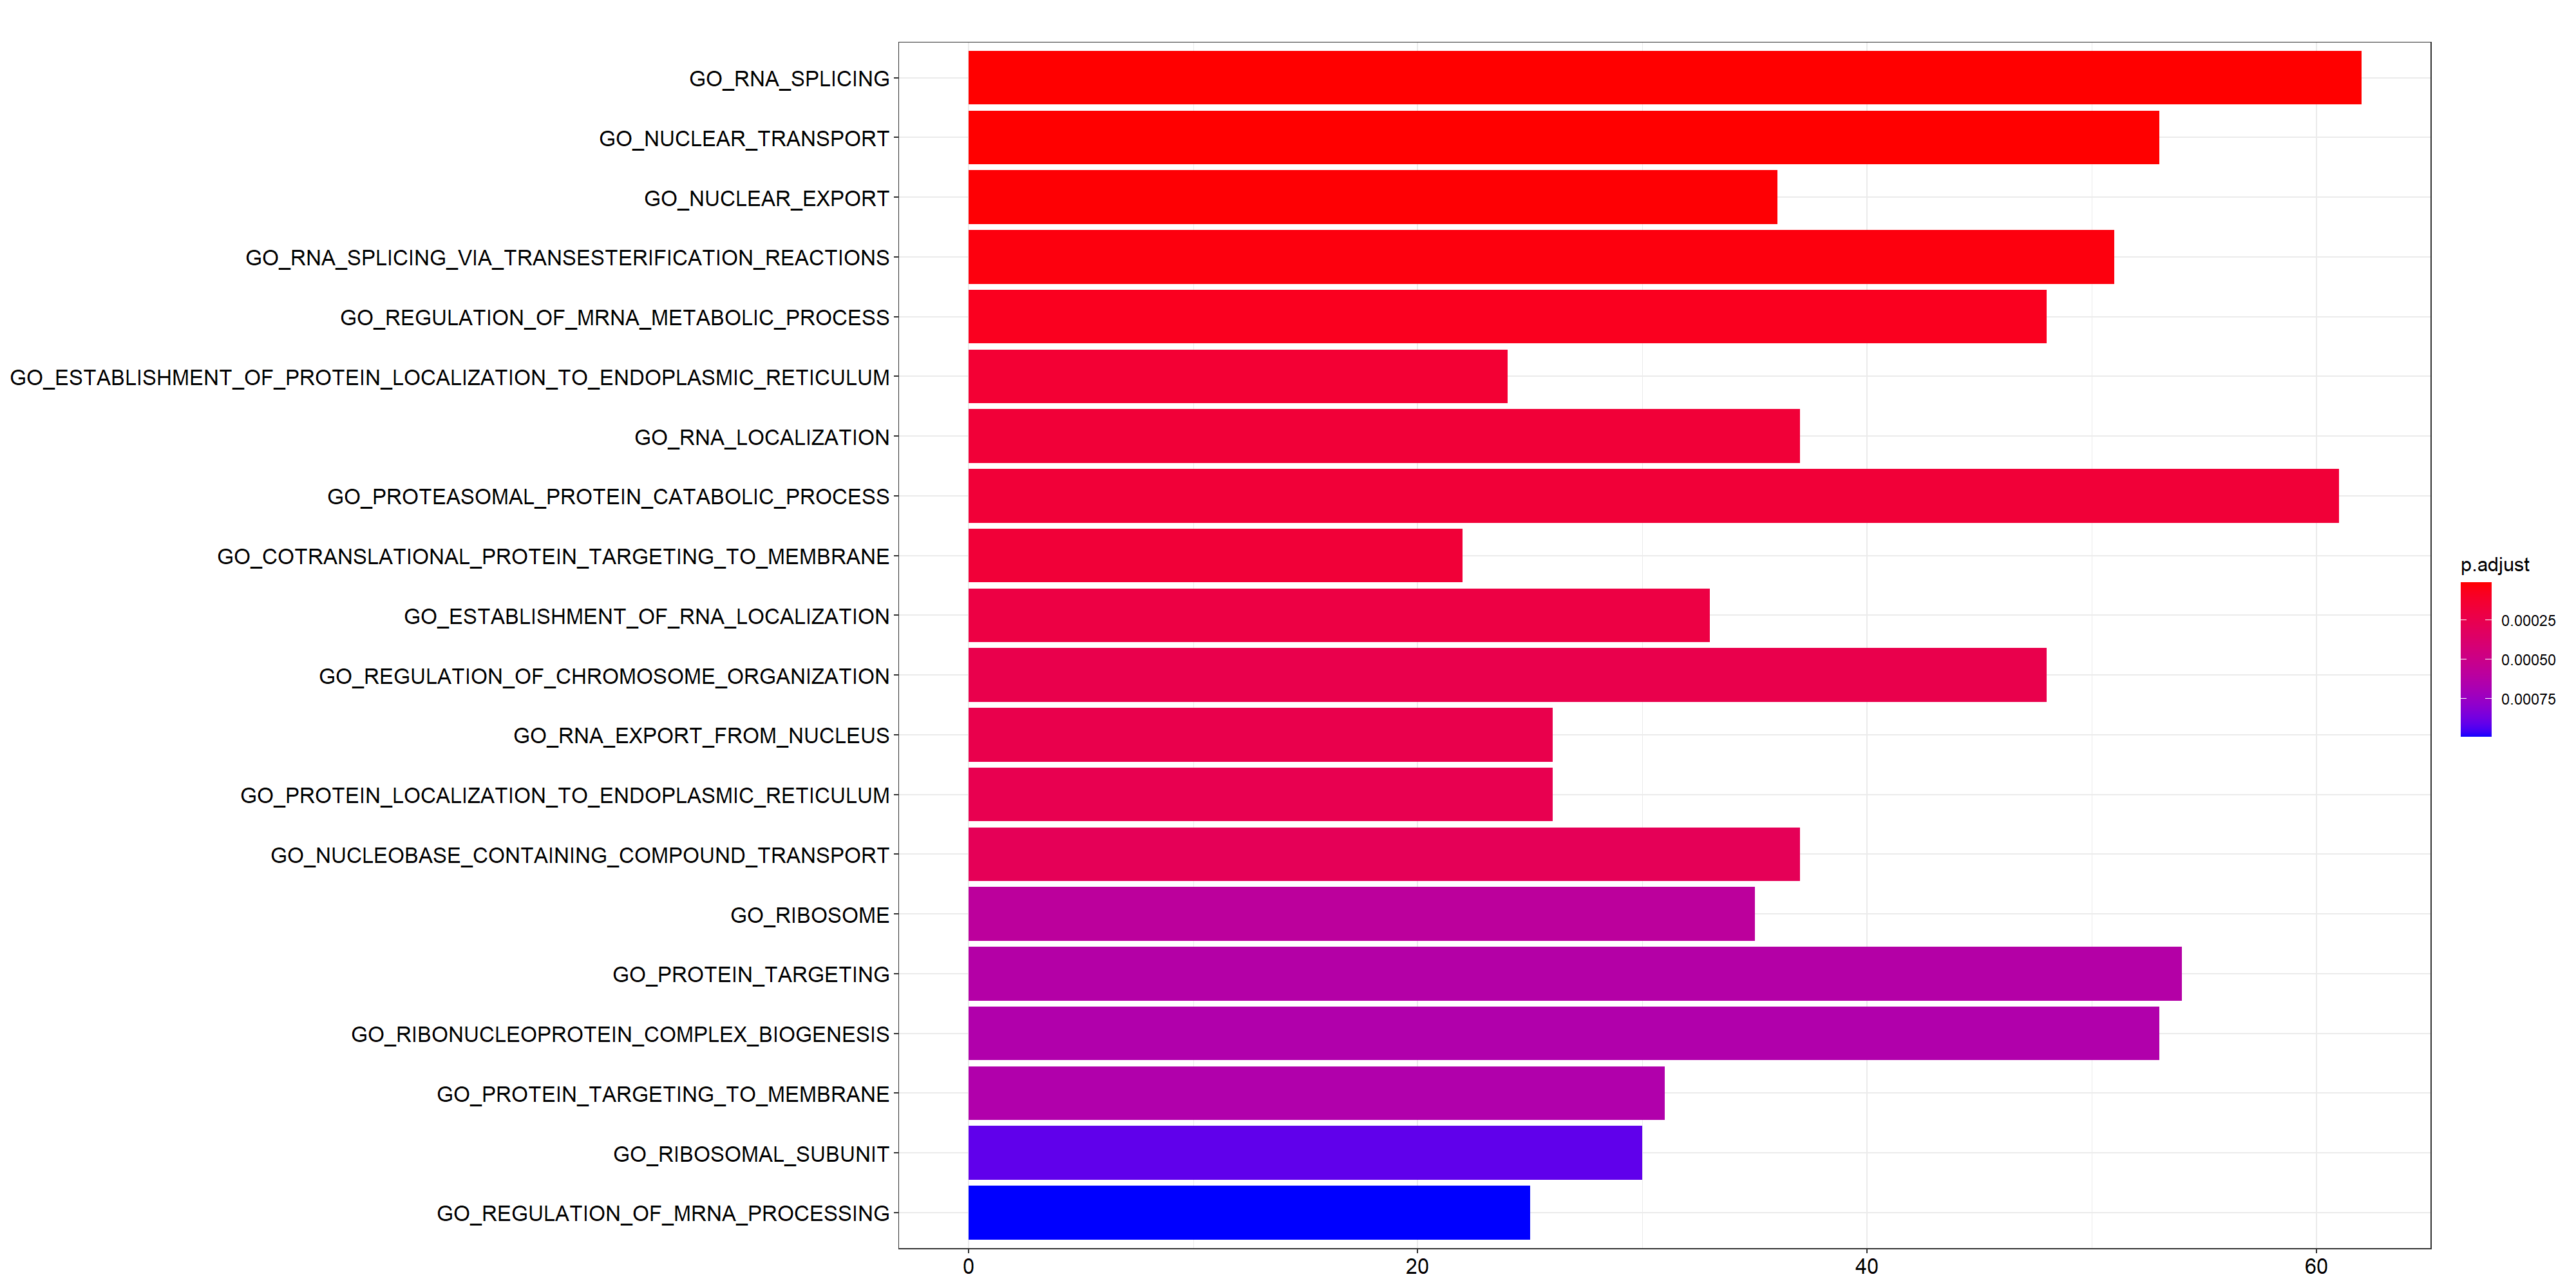
\includegraphics[width=5cm]{Figures/Path/CTLvs1_ef_barplot.png} }}%
    \qquad
    \subfloat[\centering GSEA for S1. ]{{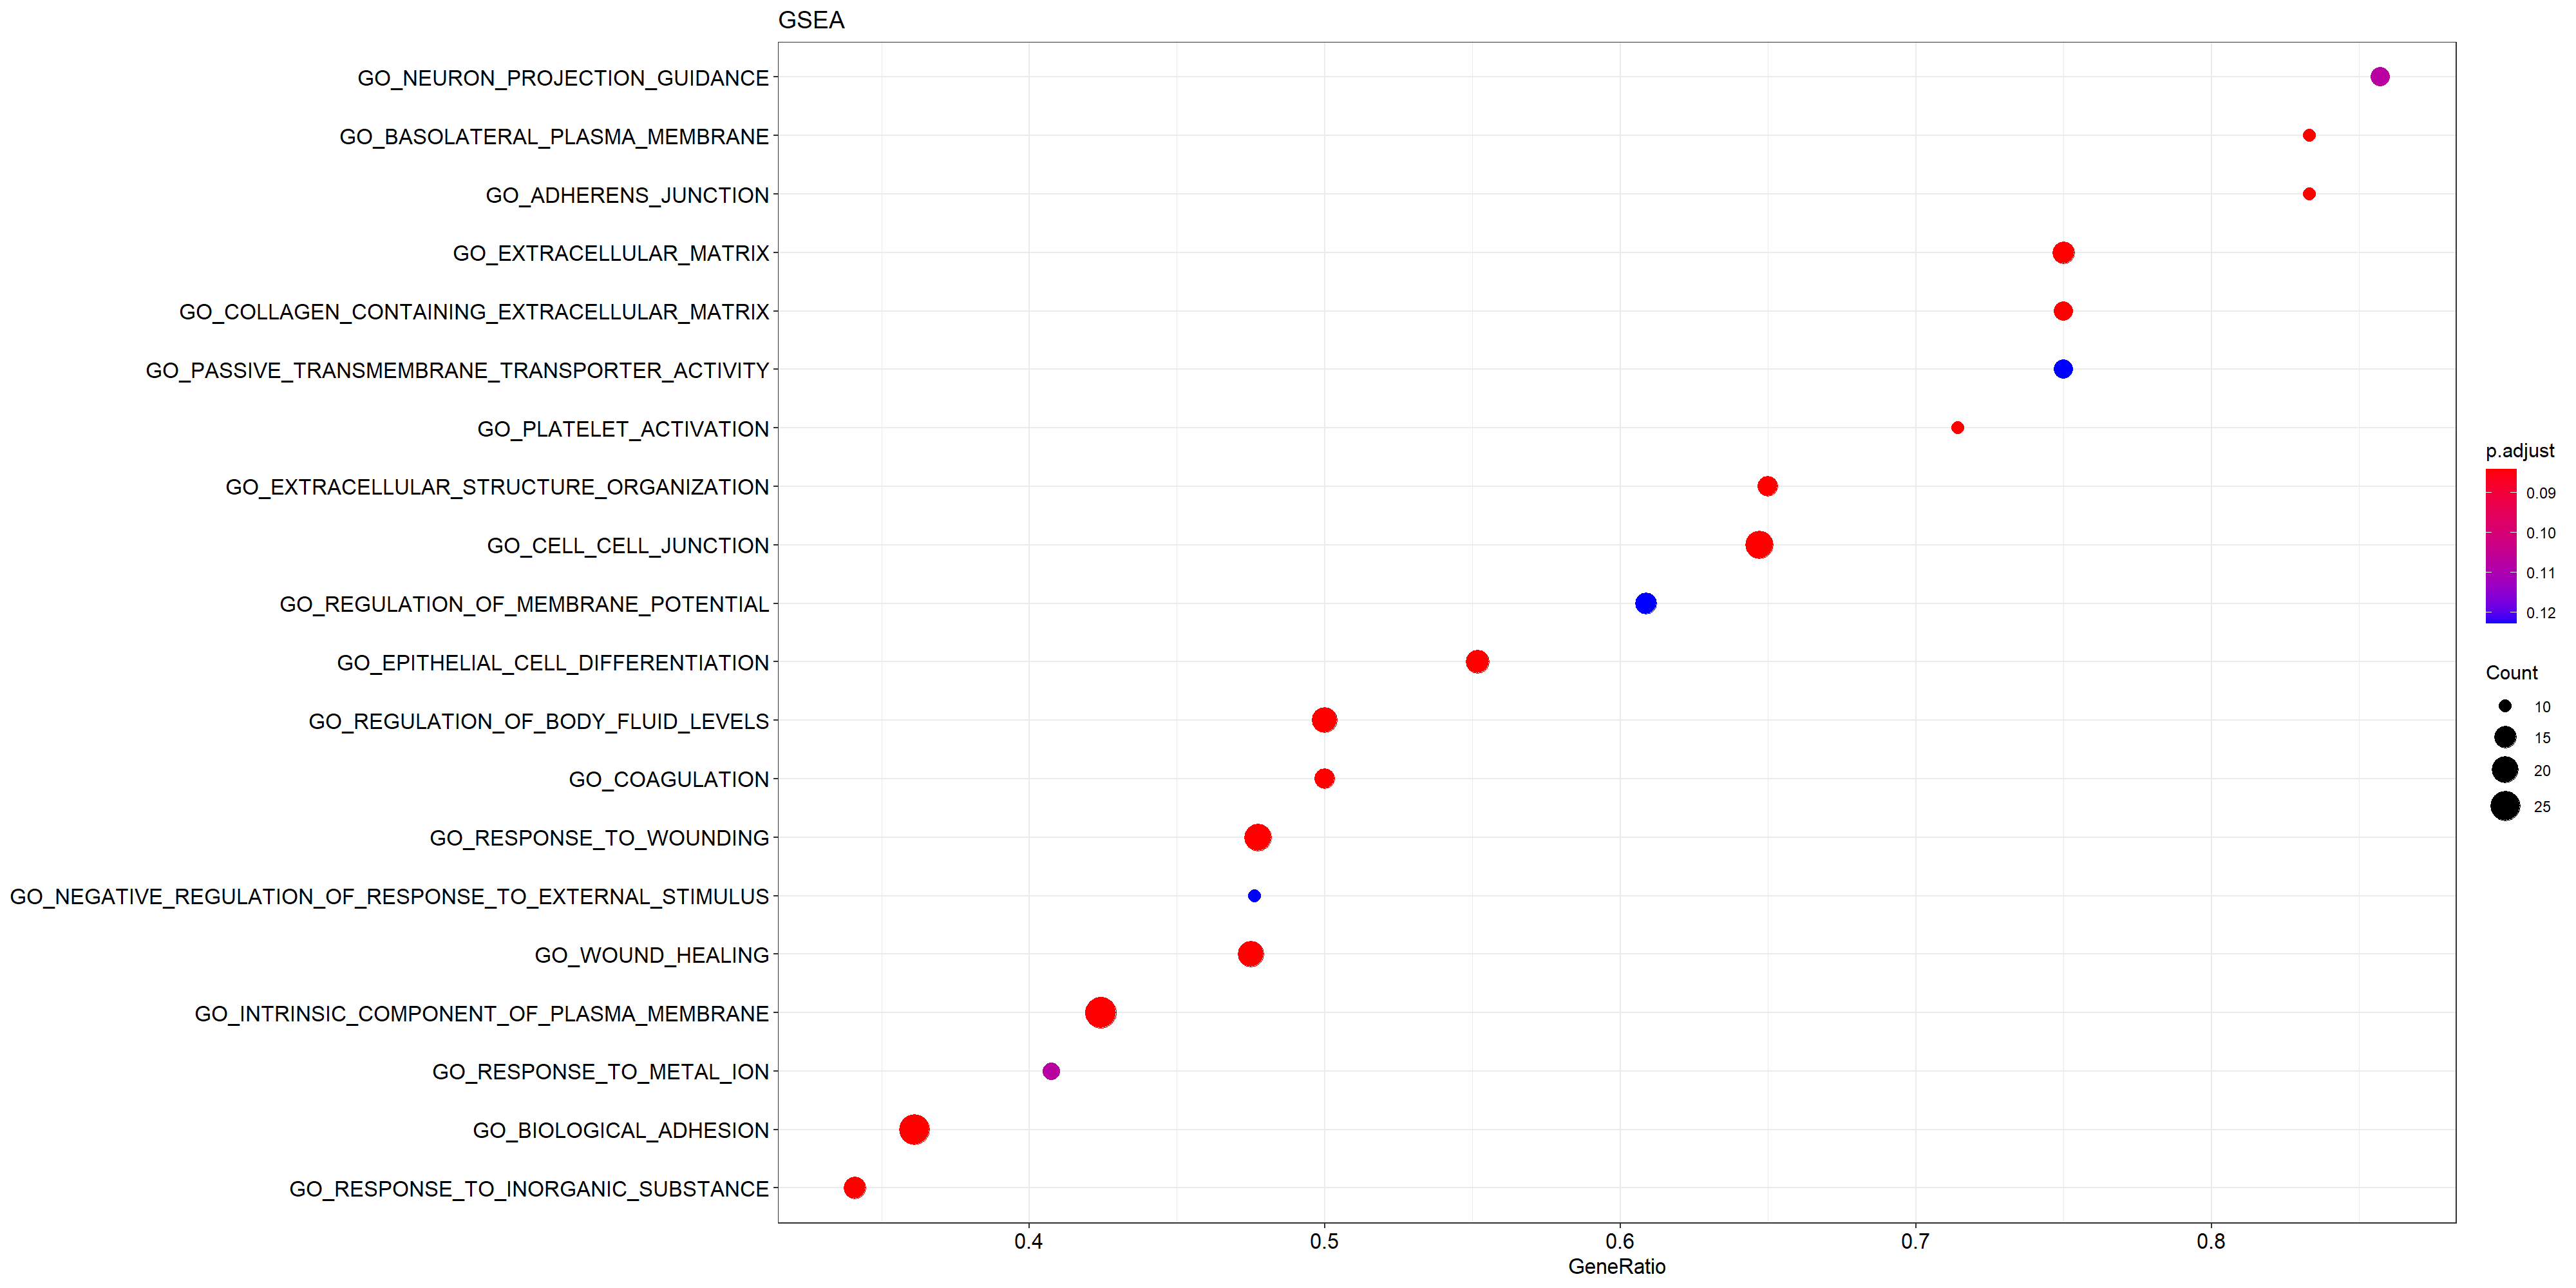
\includegraphics[width=5cm]{Figures/Path/CTLvs1_ef_dotplot.png} }}%
    \\
    \subfloat[\centering ORA for S2. ]{{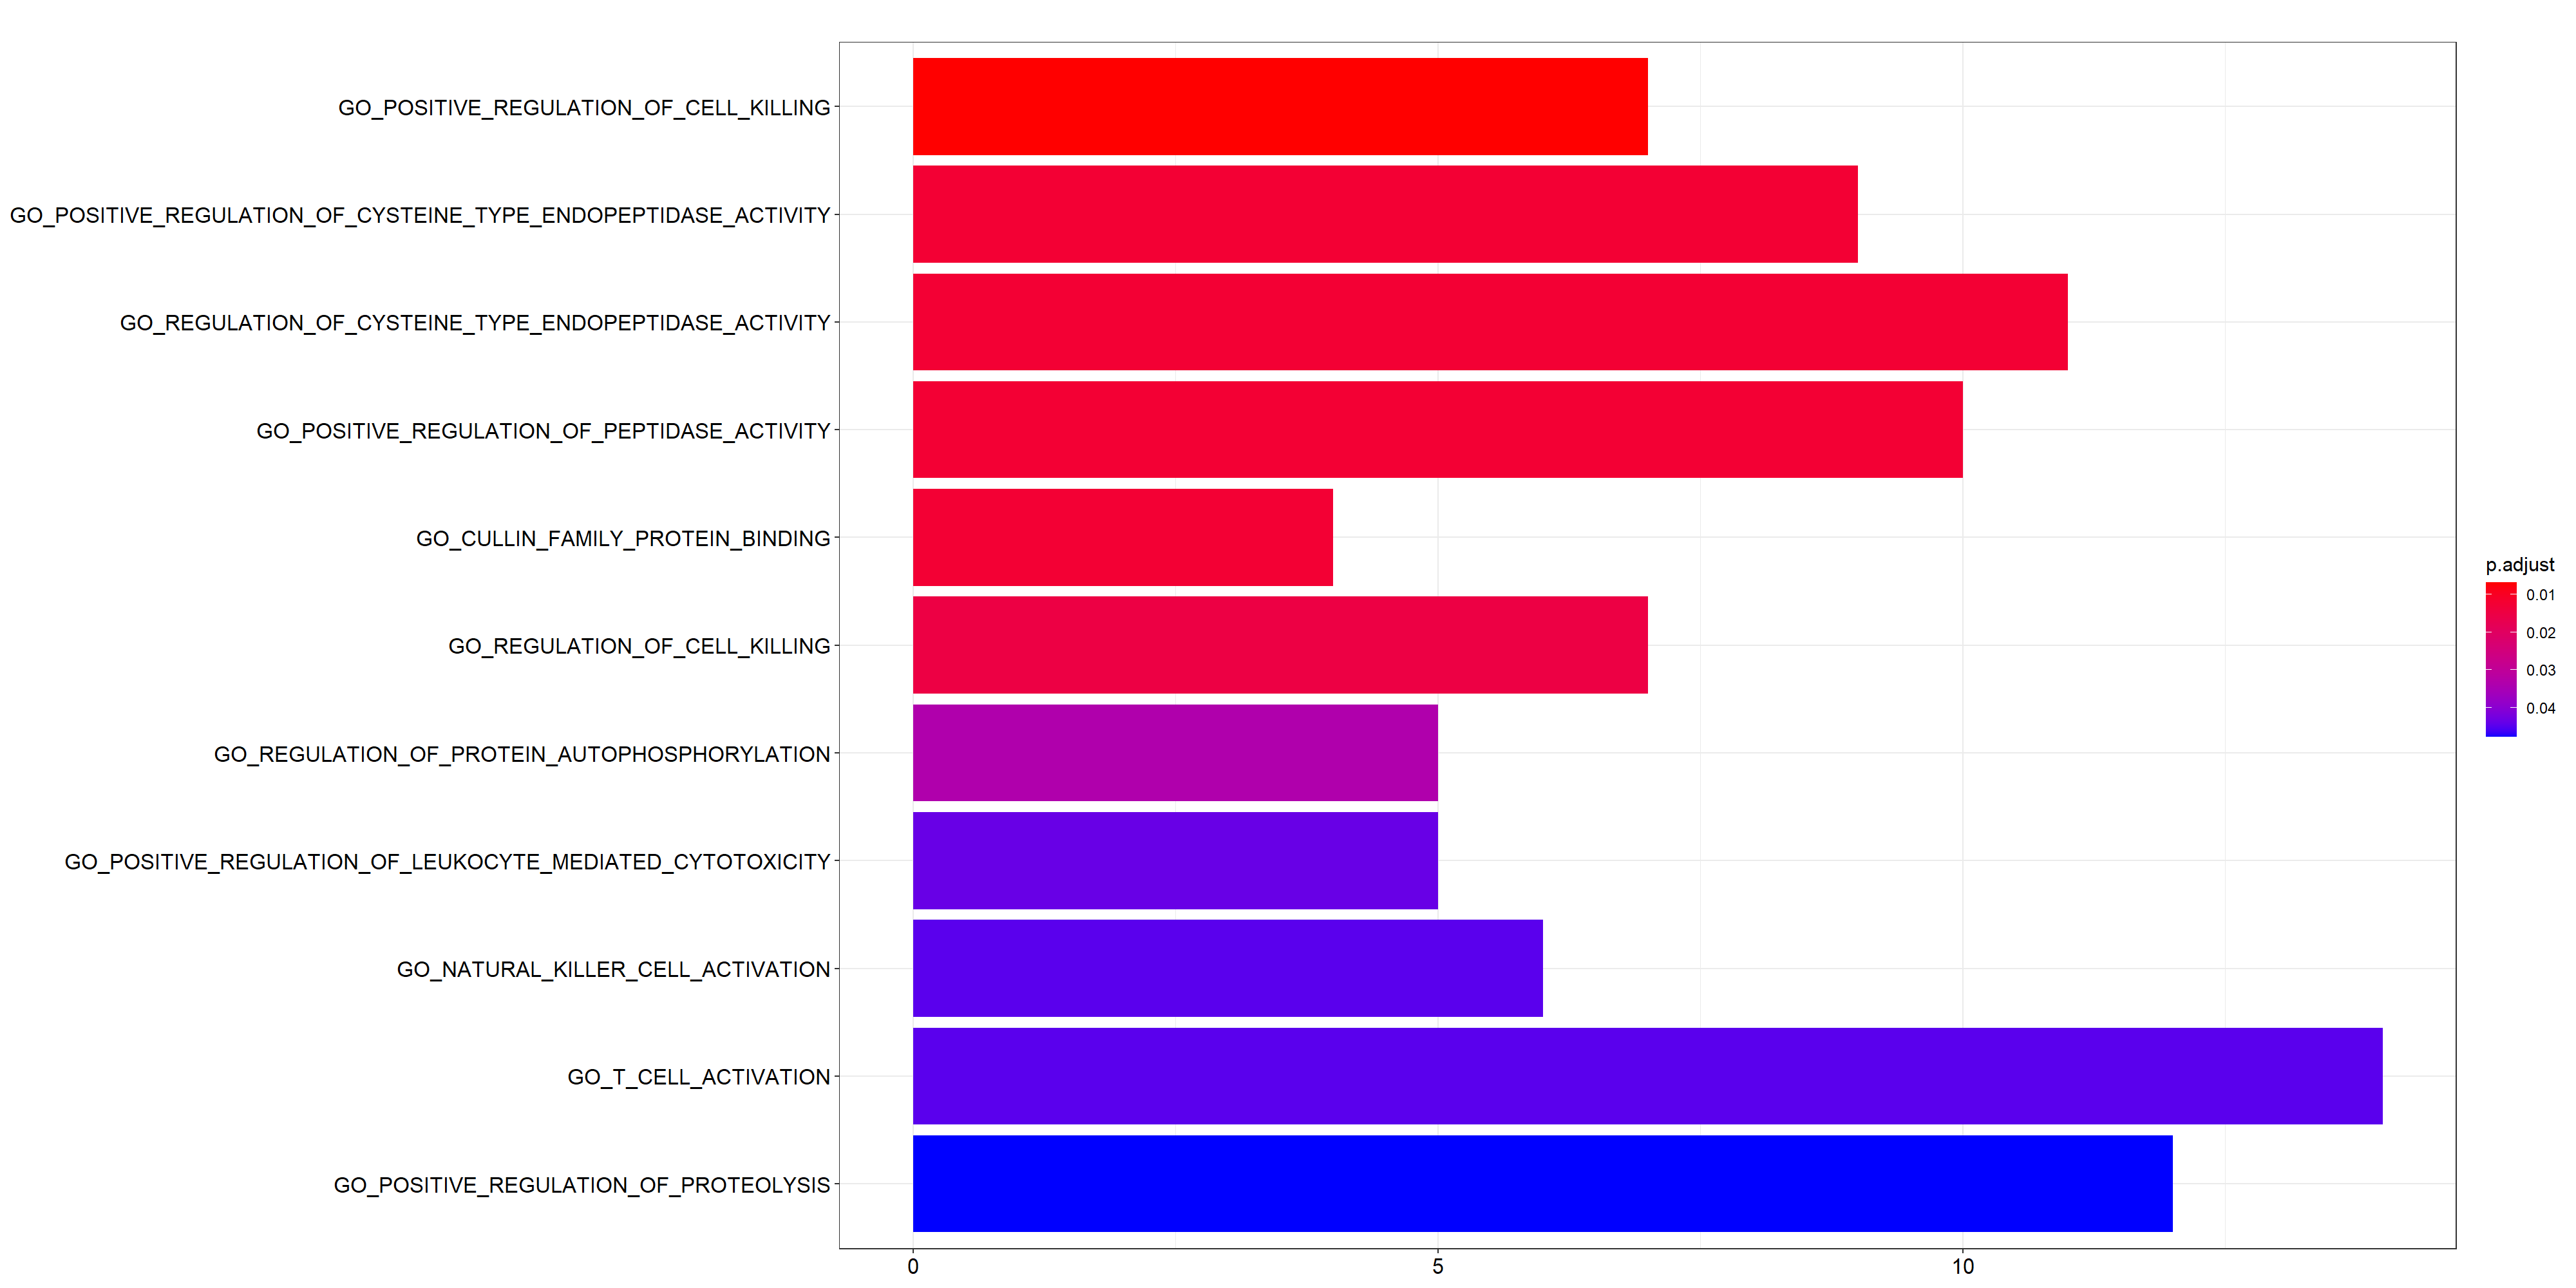
\includegraphics[width=5cm]{Figures/Path/CTLvs2_ef_barplot.png} }}%
    \qquad
    \subfloat[\centering GSEA for S2. ]{{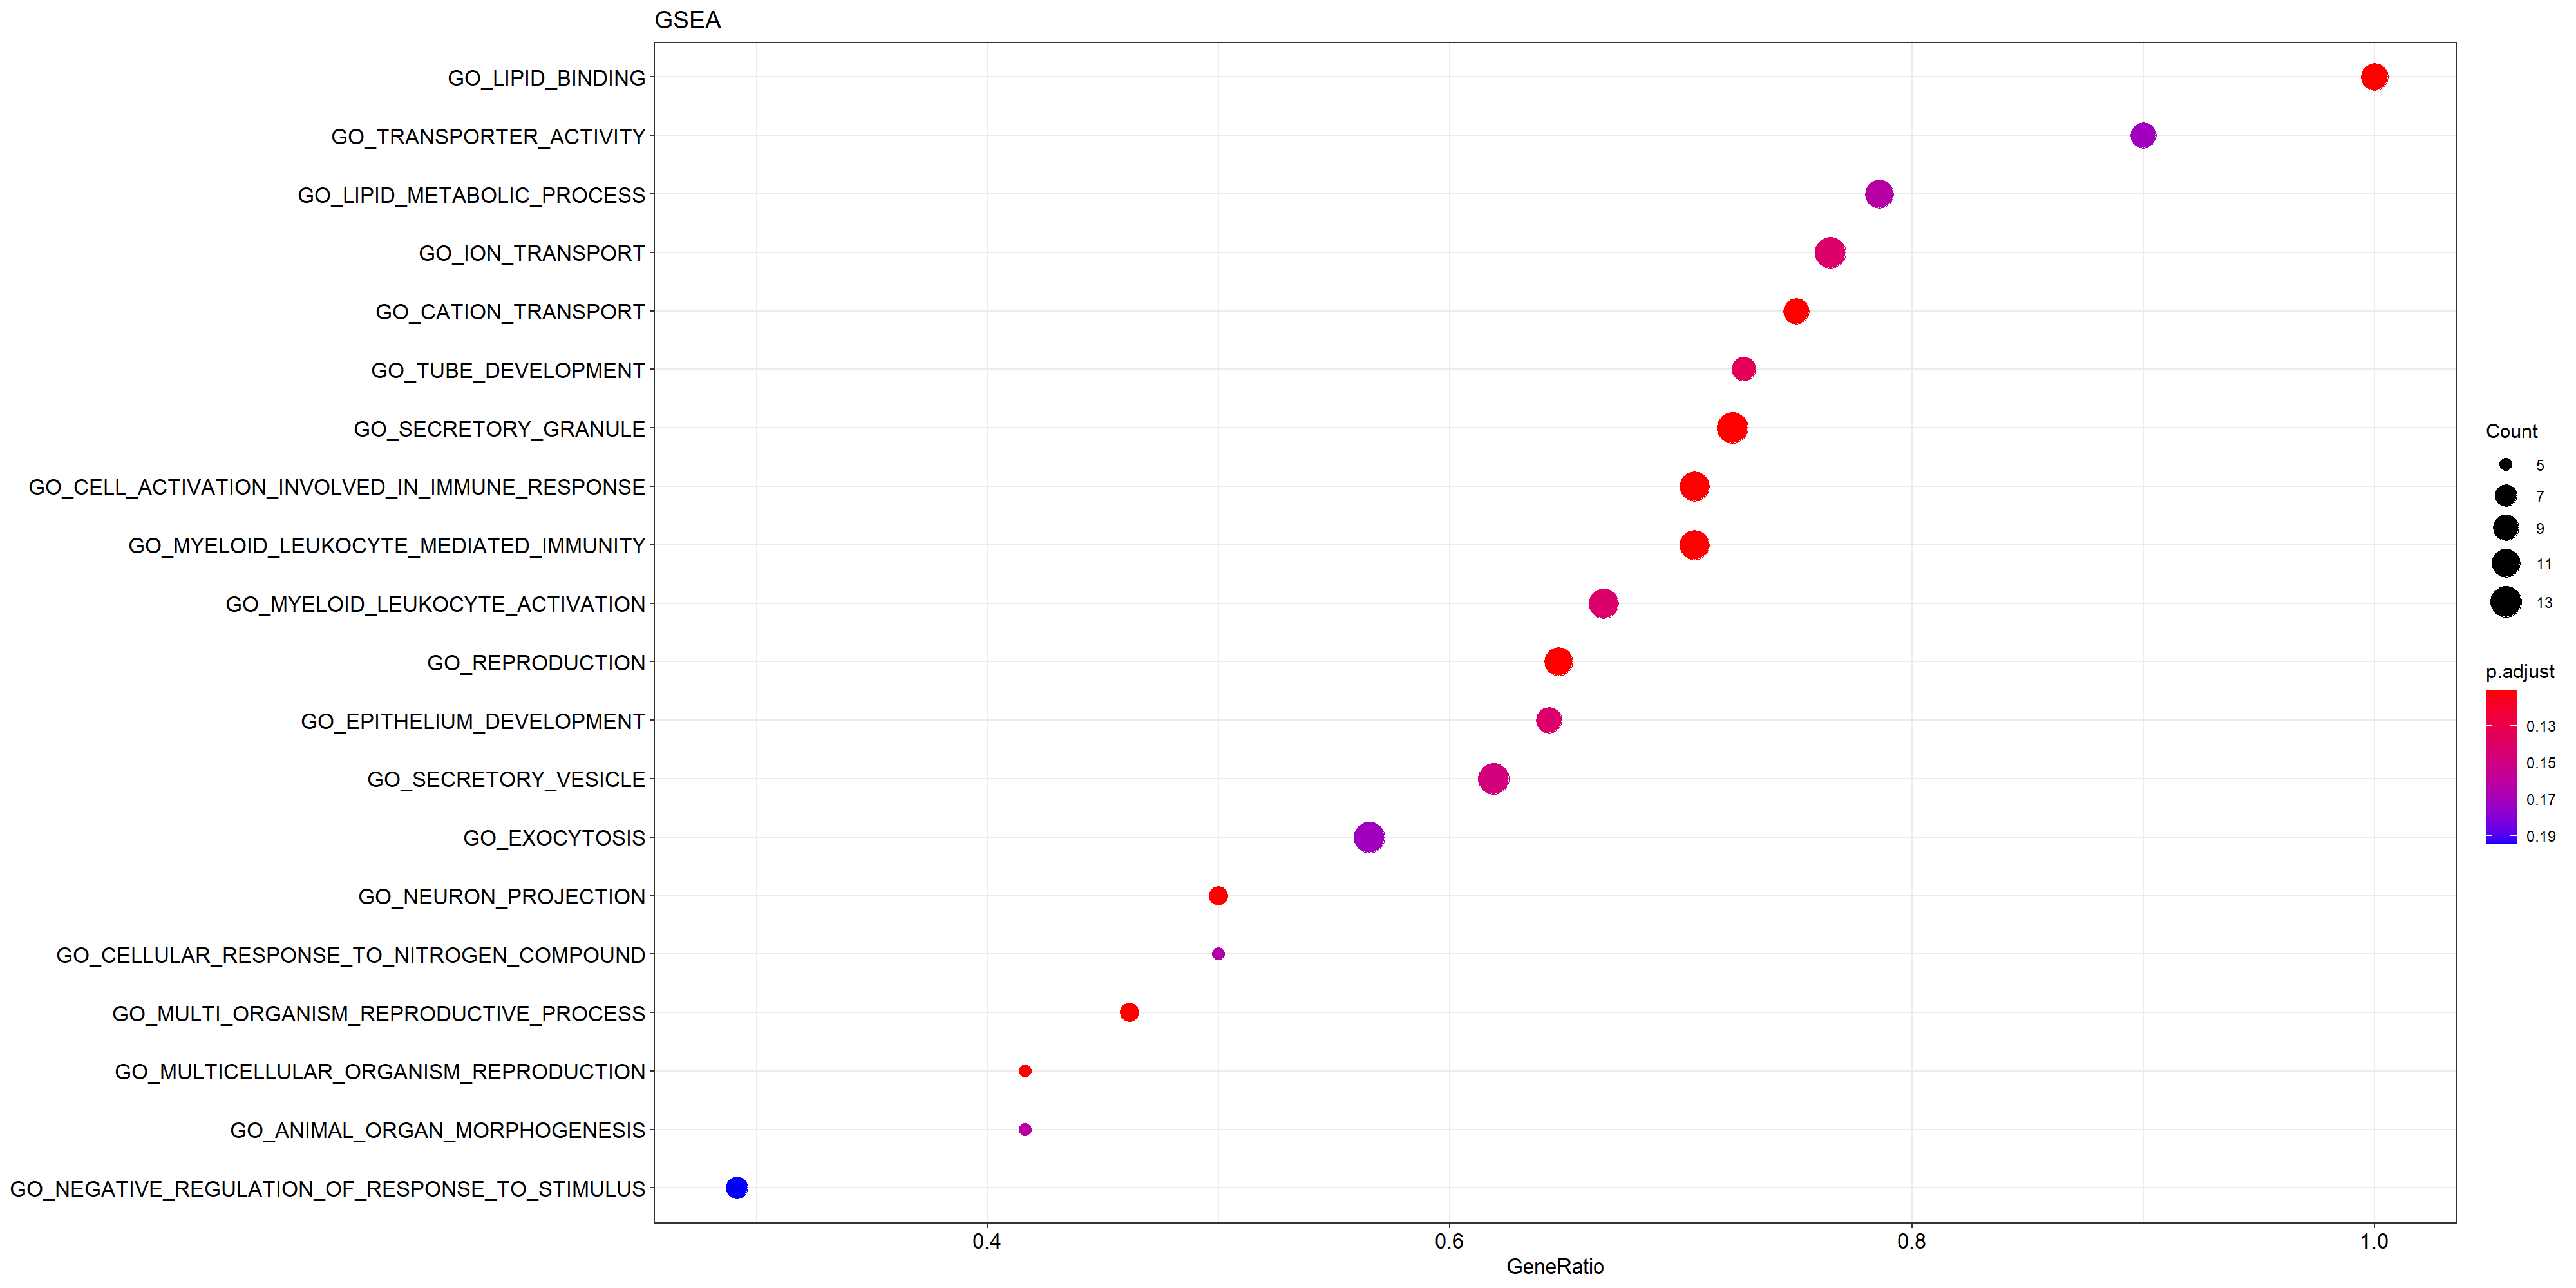
\includegraphics[width=5cm]{Figures/Path/CTLvs2_ef_dotplot.png} }}%
    \\
    \subfloat[\centering ORA for S3. ]{{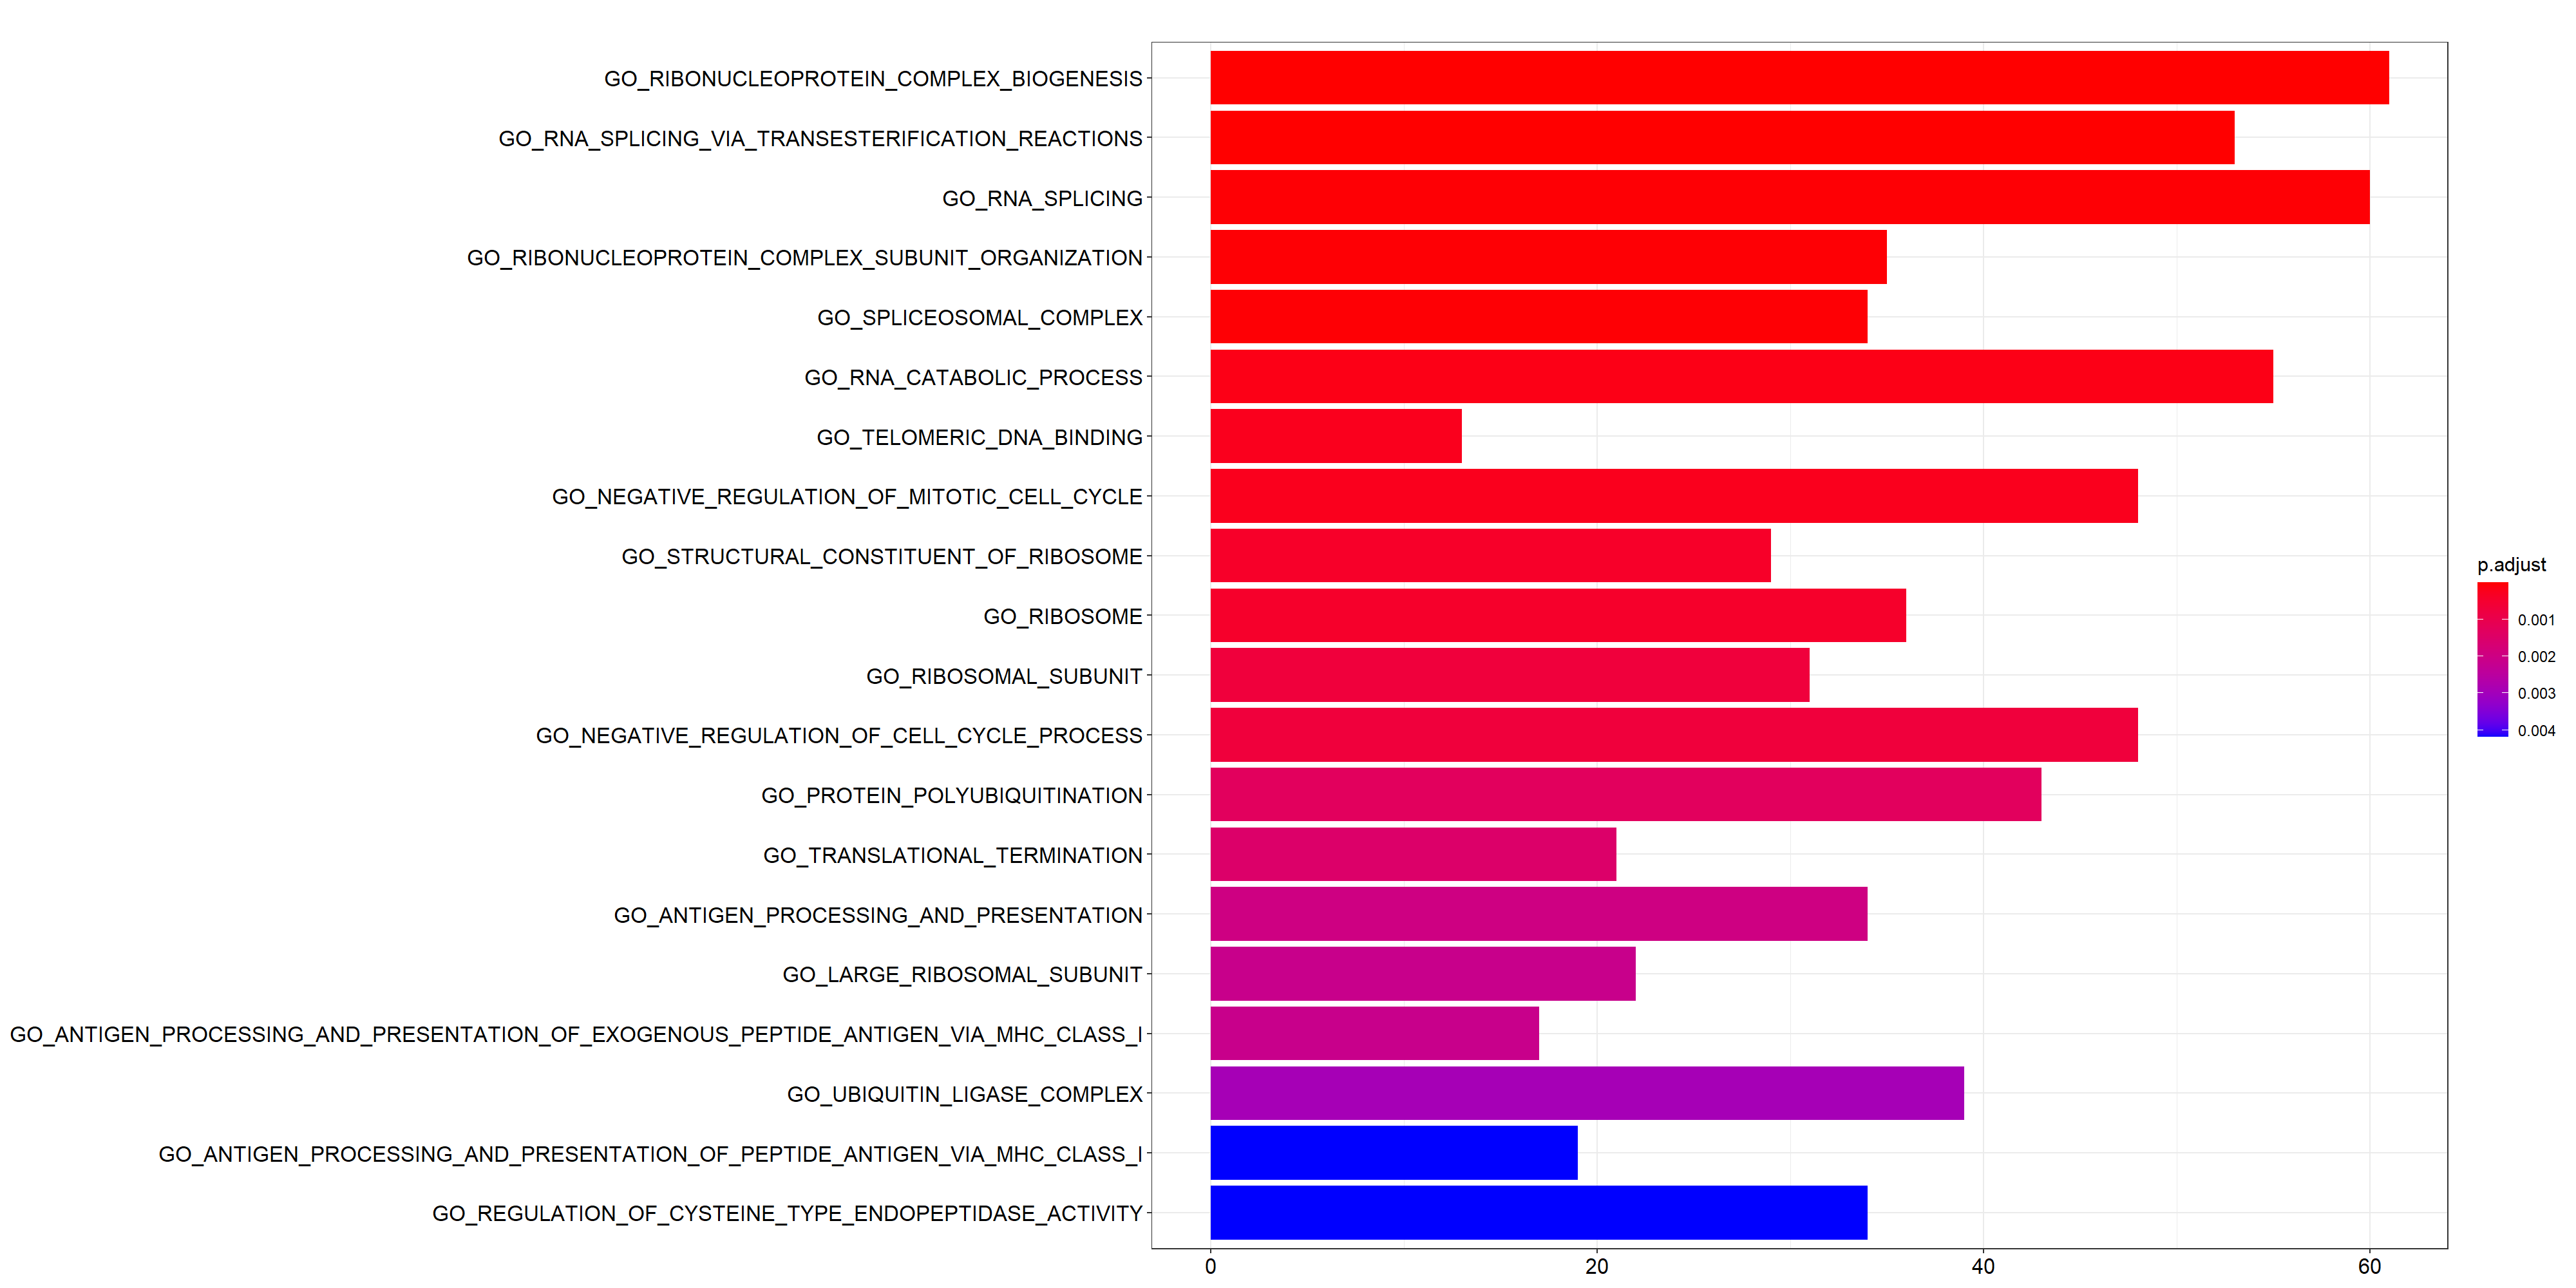
\includegraphics[width=5cm]{Figures/Path/CTLvs3_ef_barplot.png} }}%
    \qquad
    \subfloat[\centering GSEA for S3. ]{{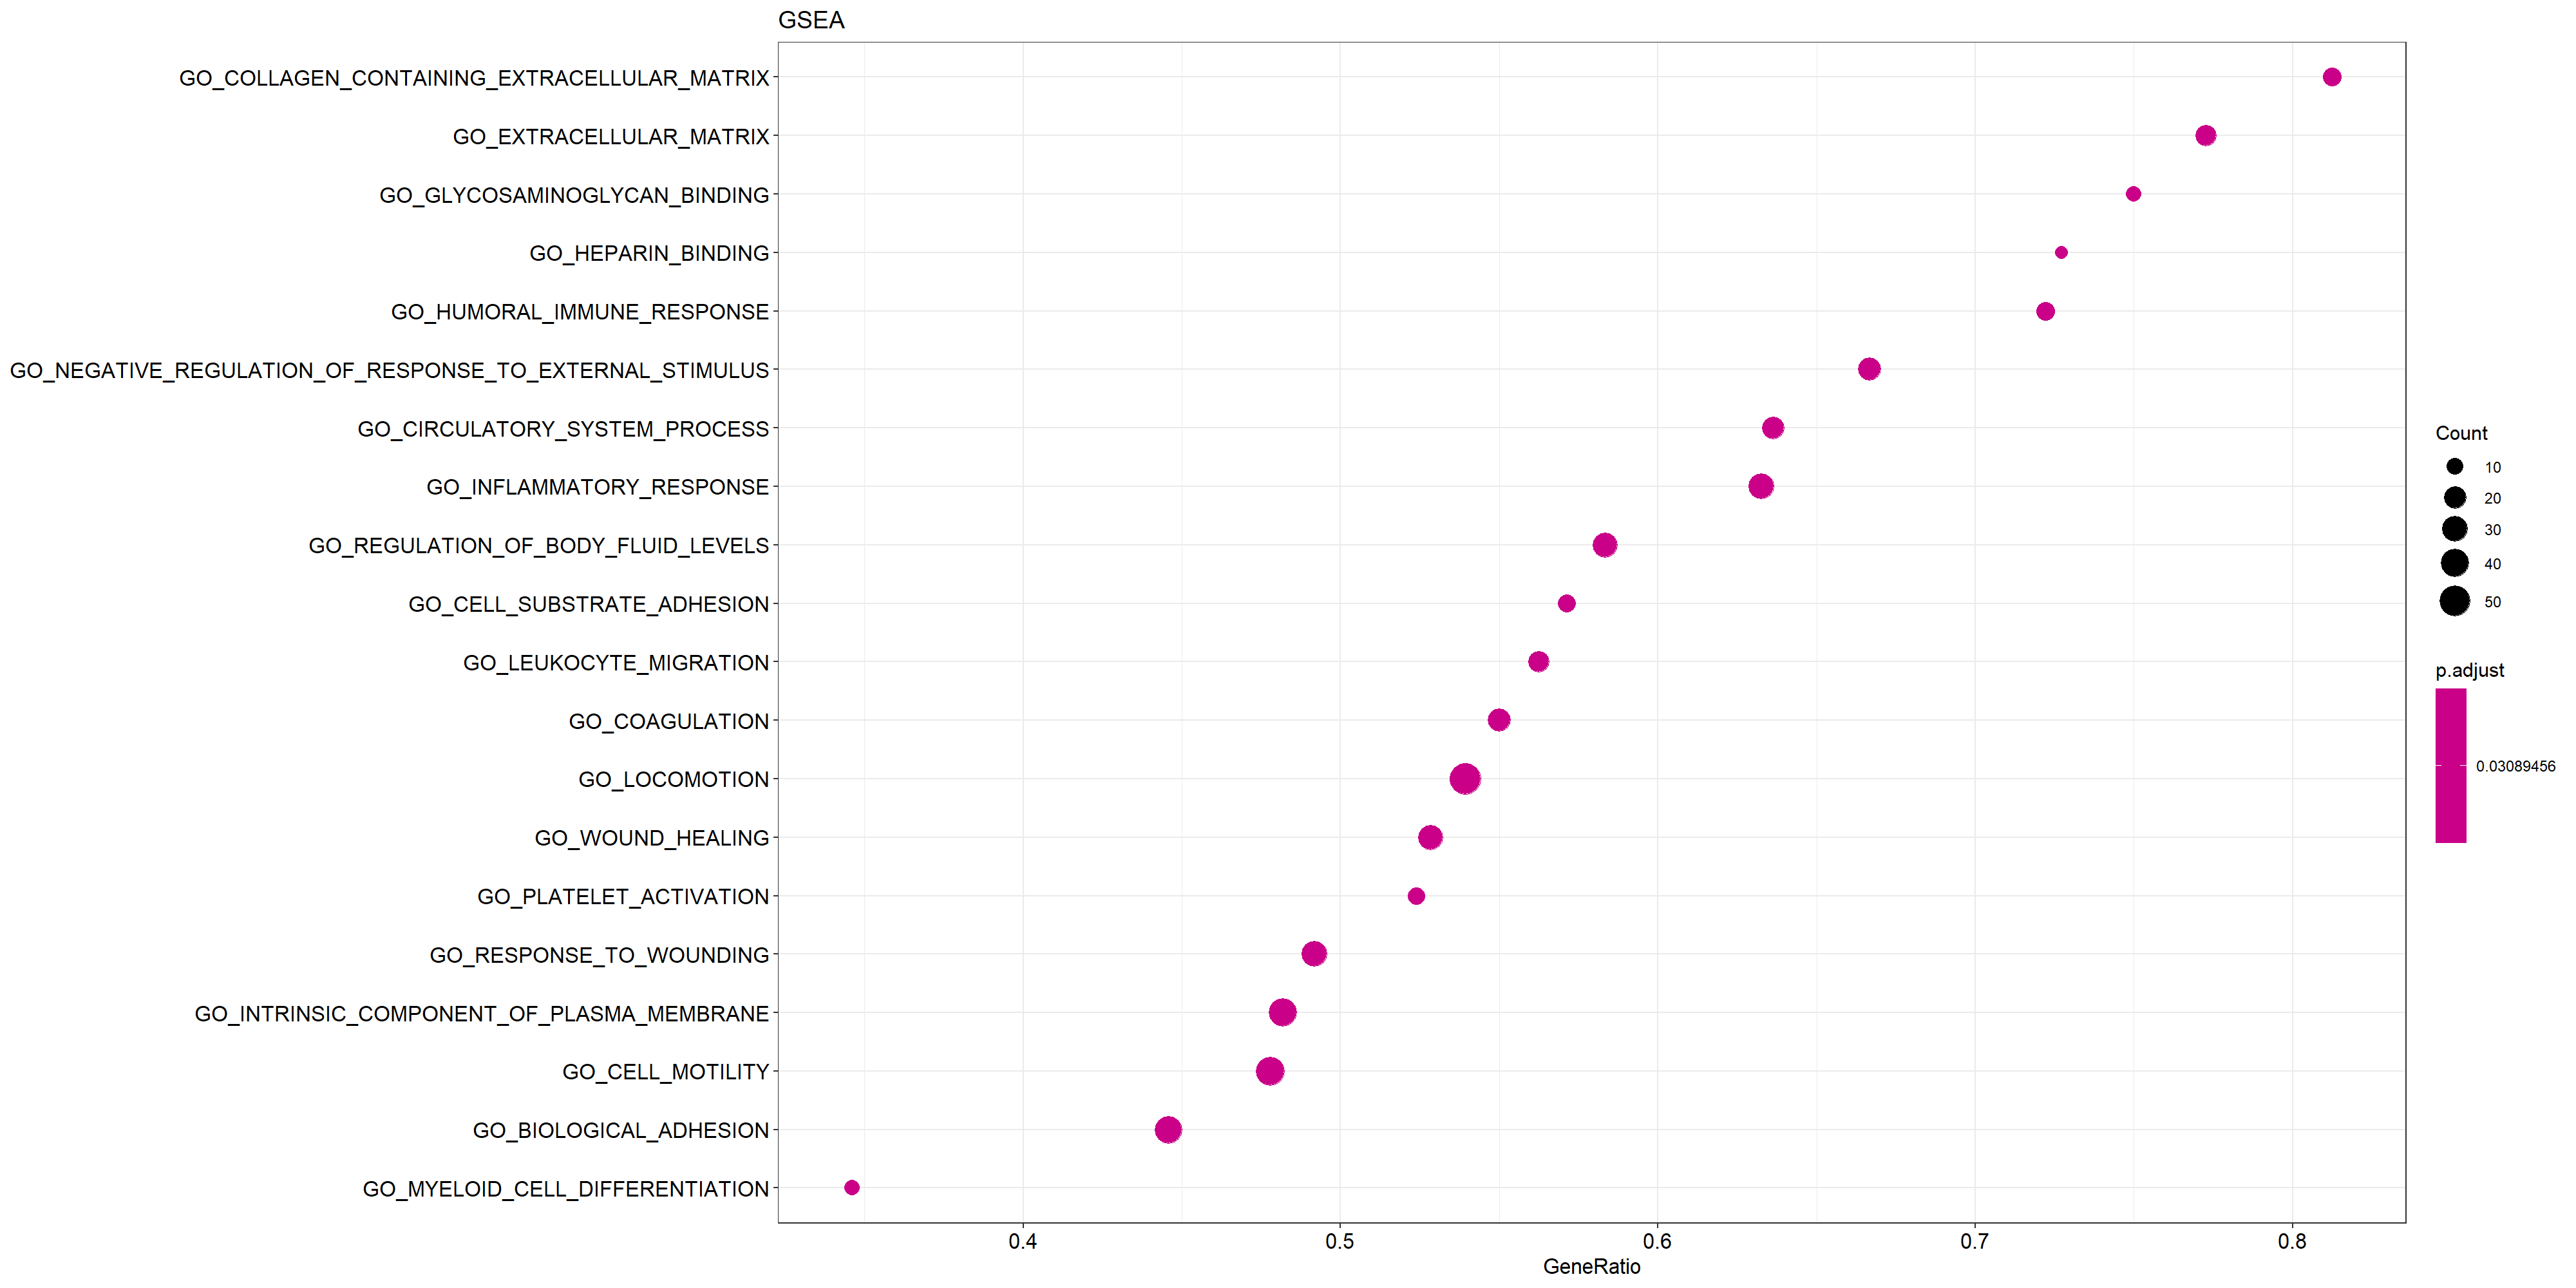
\includegraphics[width=5cm]{Figures/Path/CTLvs3_ef_dotplot.png} }}%
\caption{Bar plot and dot plot visualization for over representation analysis and gene set enrichment analysis, respectively, of sutbype in Blood-HD-f.}
\label{fig:path-blood-f-sub}%
\end{figure}

On the other hand, according to ORA results, the male sutbype 1 has linked pathways about macroauthophagy/ autophagy processes, catabolic procesess, ubiquitination, and RNA splicing. Subtype 2 is also related to autophagy, RNA splicing, intracellular transport, and chromosome region (see Fig. \ref{fig:path-blood-m-sub}). Moreover, for GSEA, subtype 1 contained mainly immune system related pathways, specially with leukocytes, and autophagy. Likewise, S2 included pathways associated with immune system processes, neuroinflammation response, and glial cell activation. 

\begin{figure}[!ht]%
    \centering
    \subfloat[\centering ORA for S1. ]{{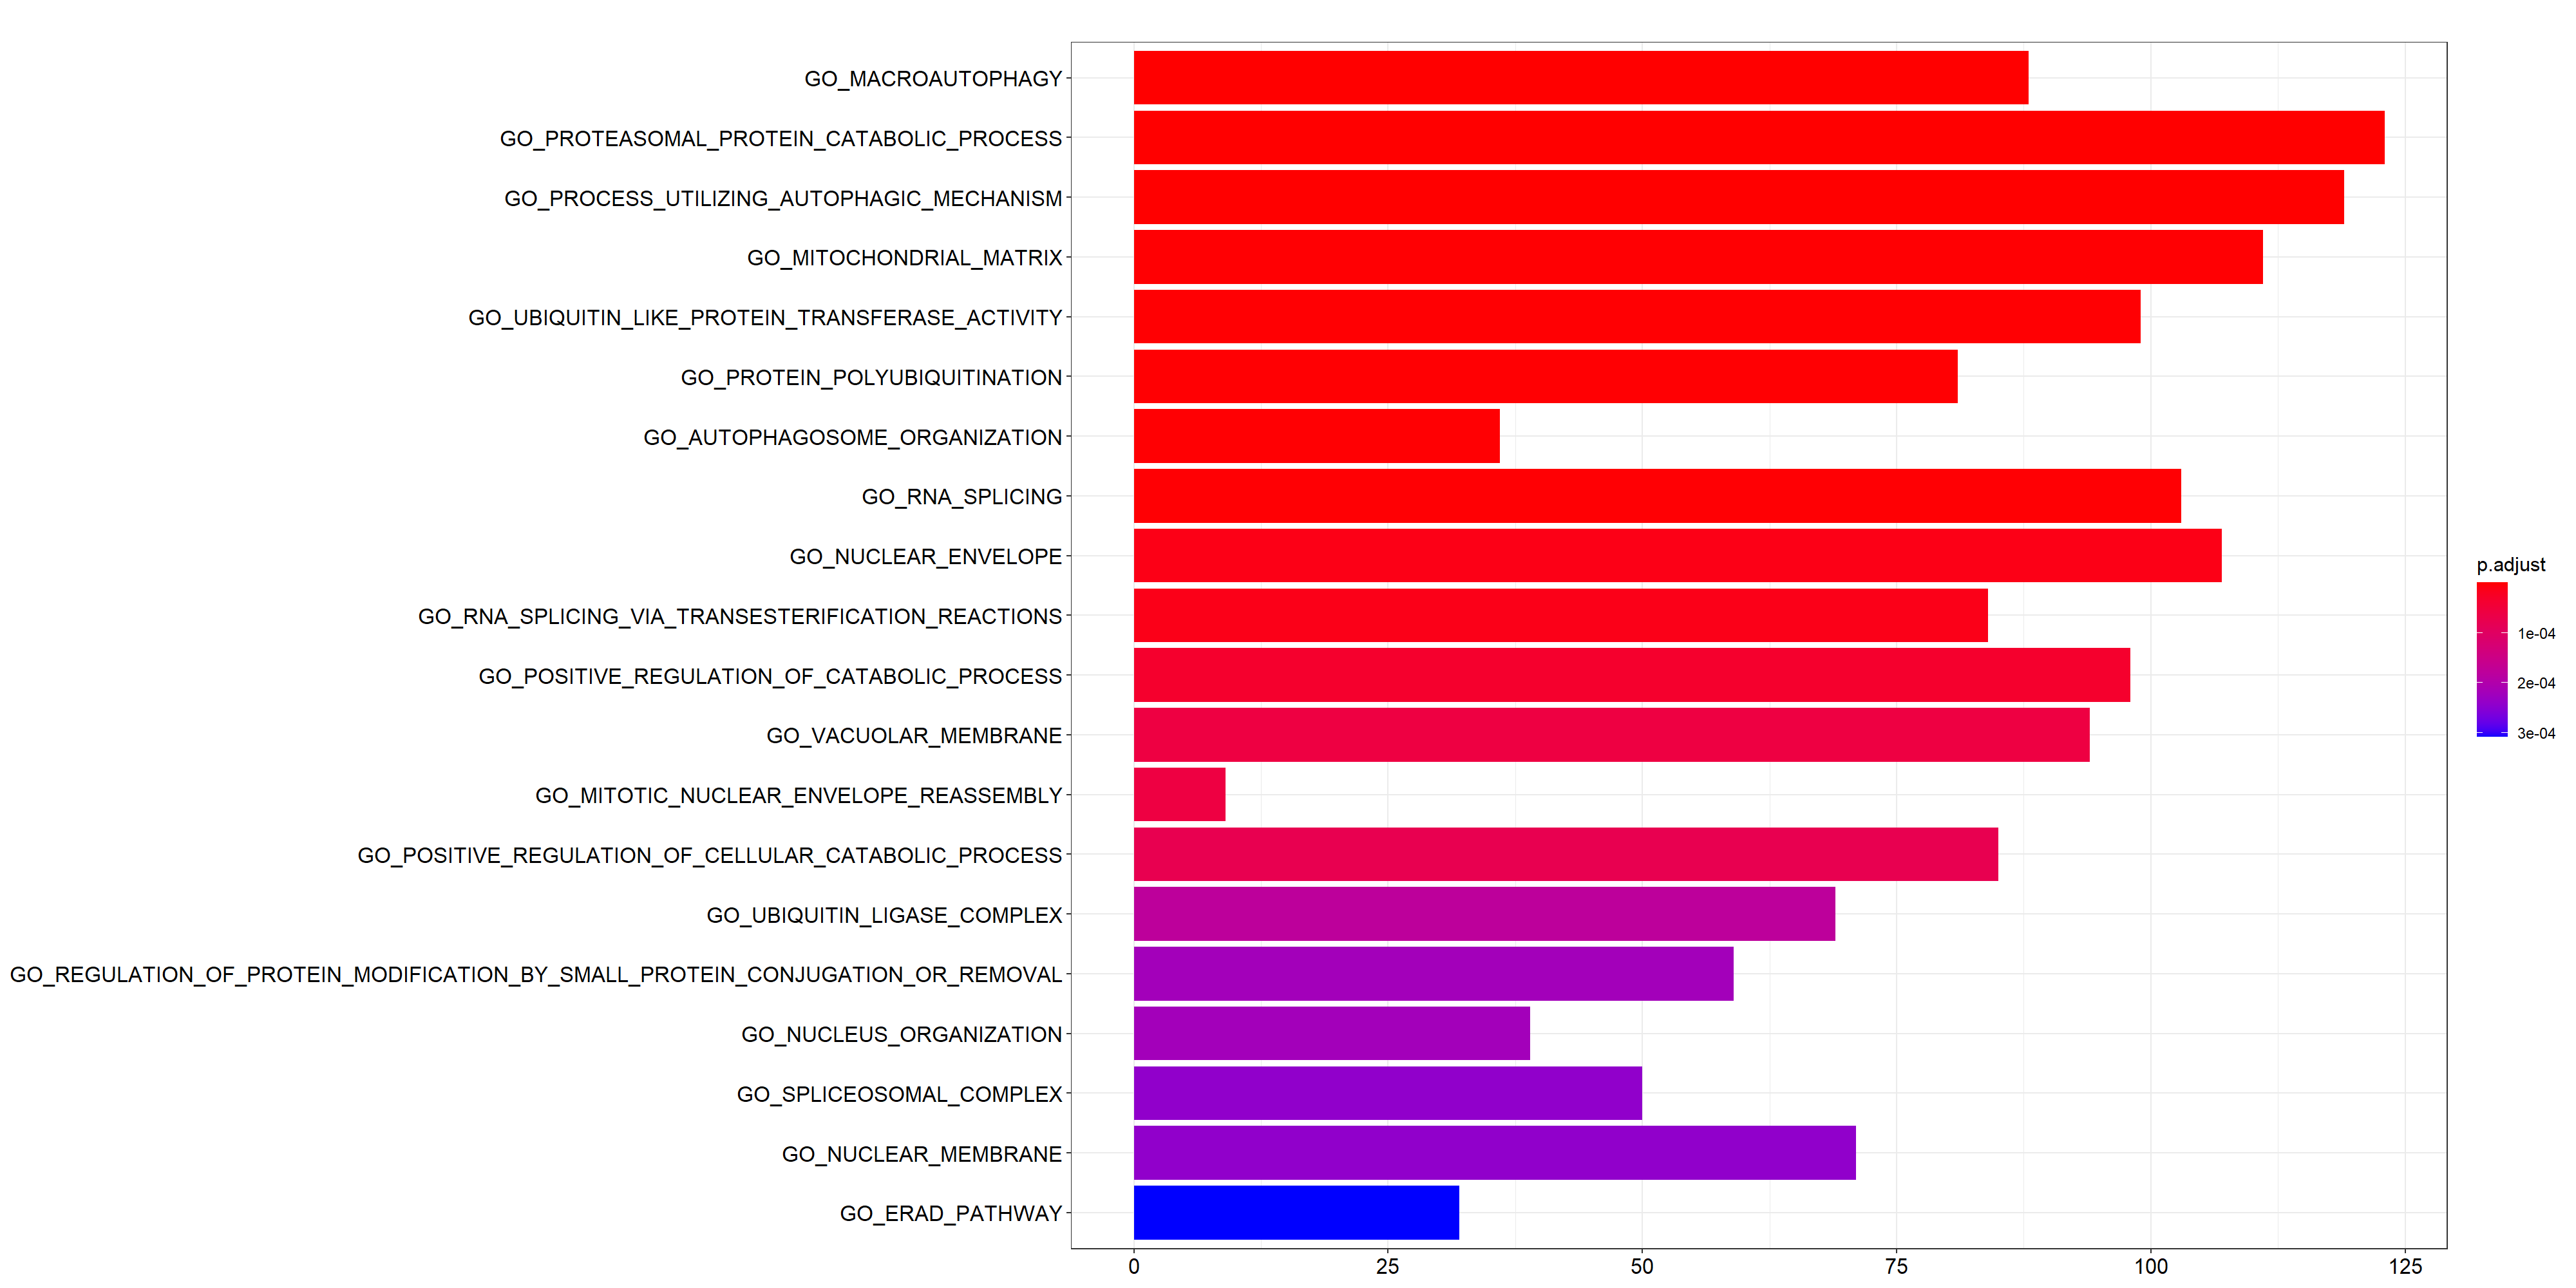
\includegraphics[width=5cm]{Figures/Path/CTLvs1_em_barplot.png} }}%
    \qquad
    \subfloat[\centering GSEA for S1. ]{{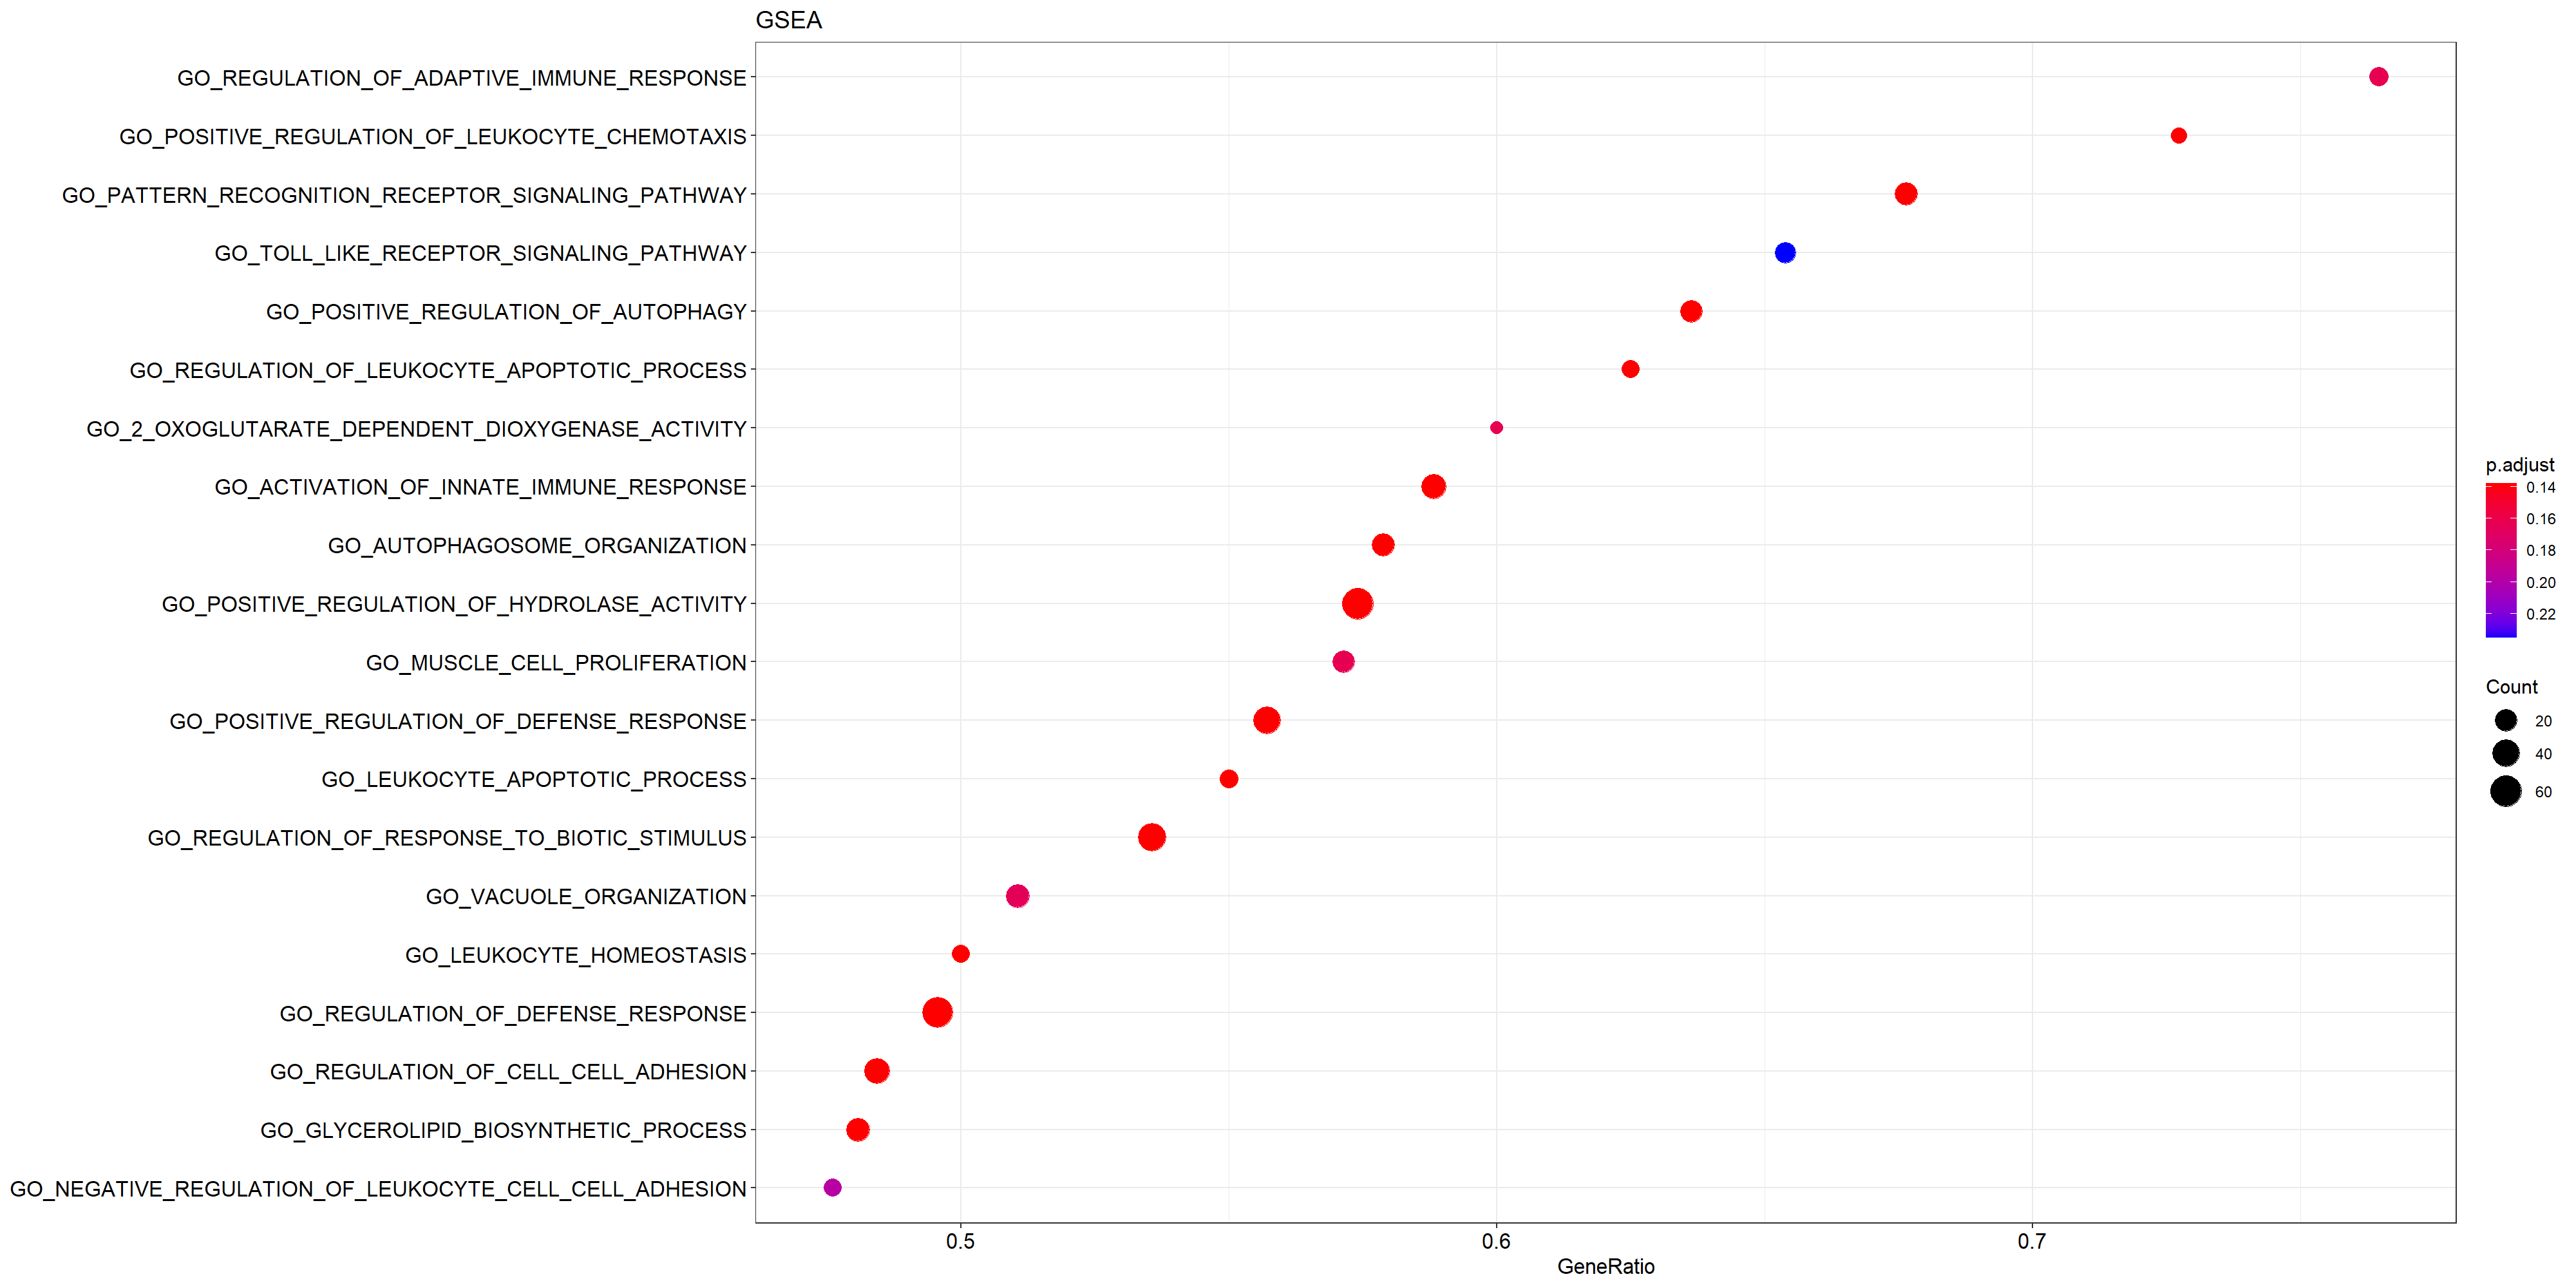
\includegraphics[width=5cm]{Figures/Path/CTLvs1_em_dotplot.png} }}%
    \\
    \subfloat[\centering ORA for S2. ]{{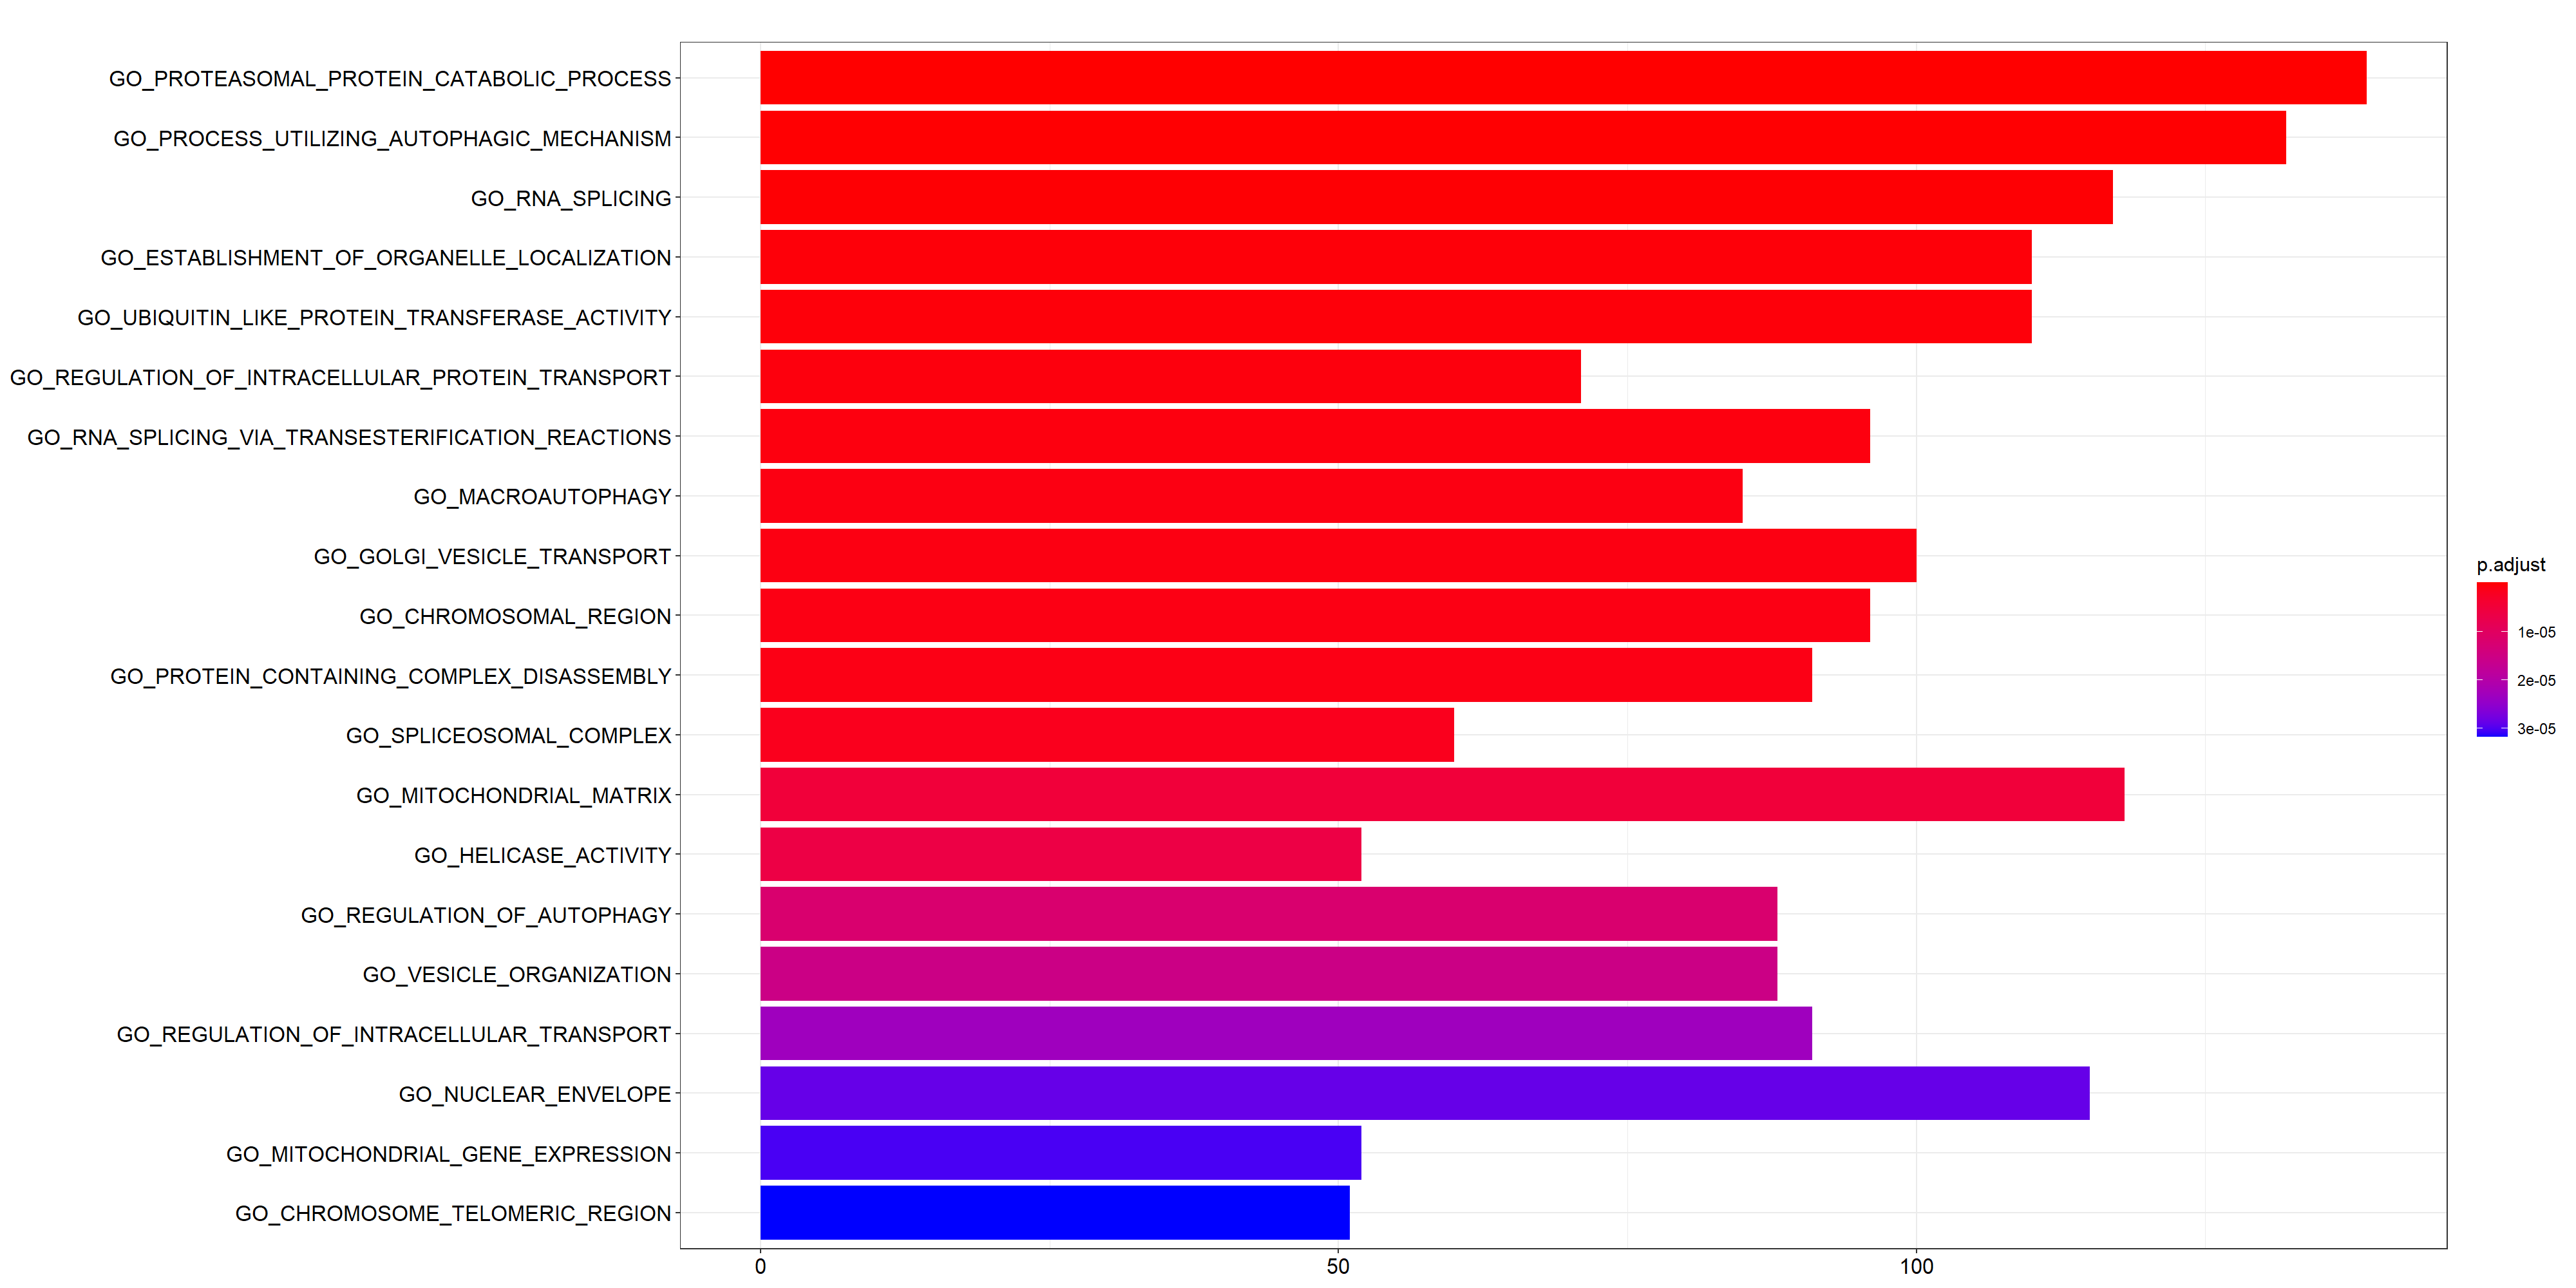
\includegraphics[width=5cm]{Figures/Path/CTLvs2_em_barplot.png} }}%
    \qquad
    \subfloat[\centering GSEA for S2. ]{{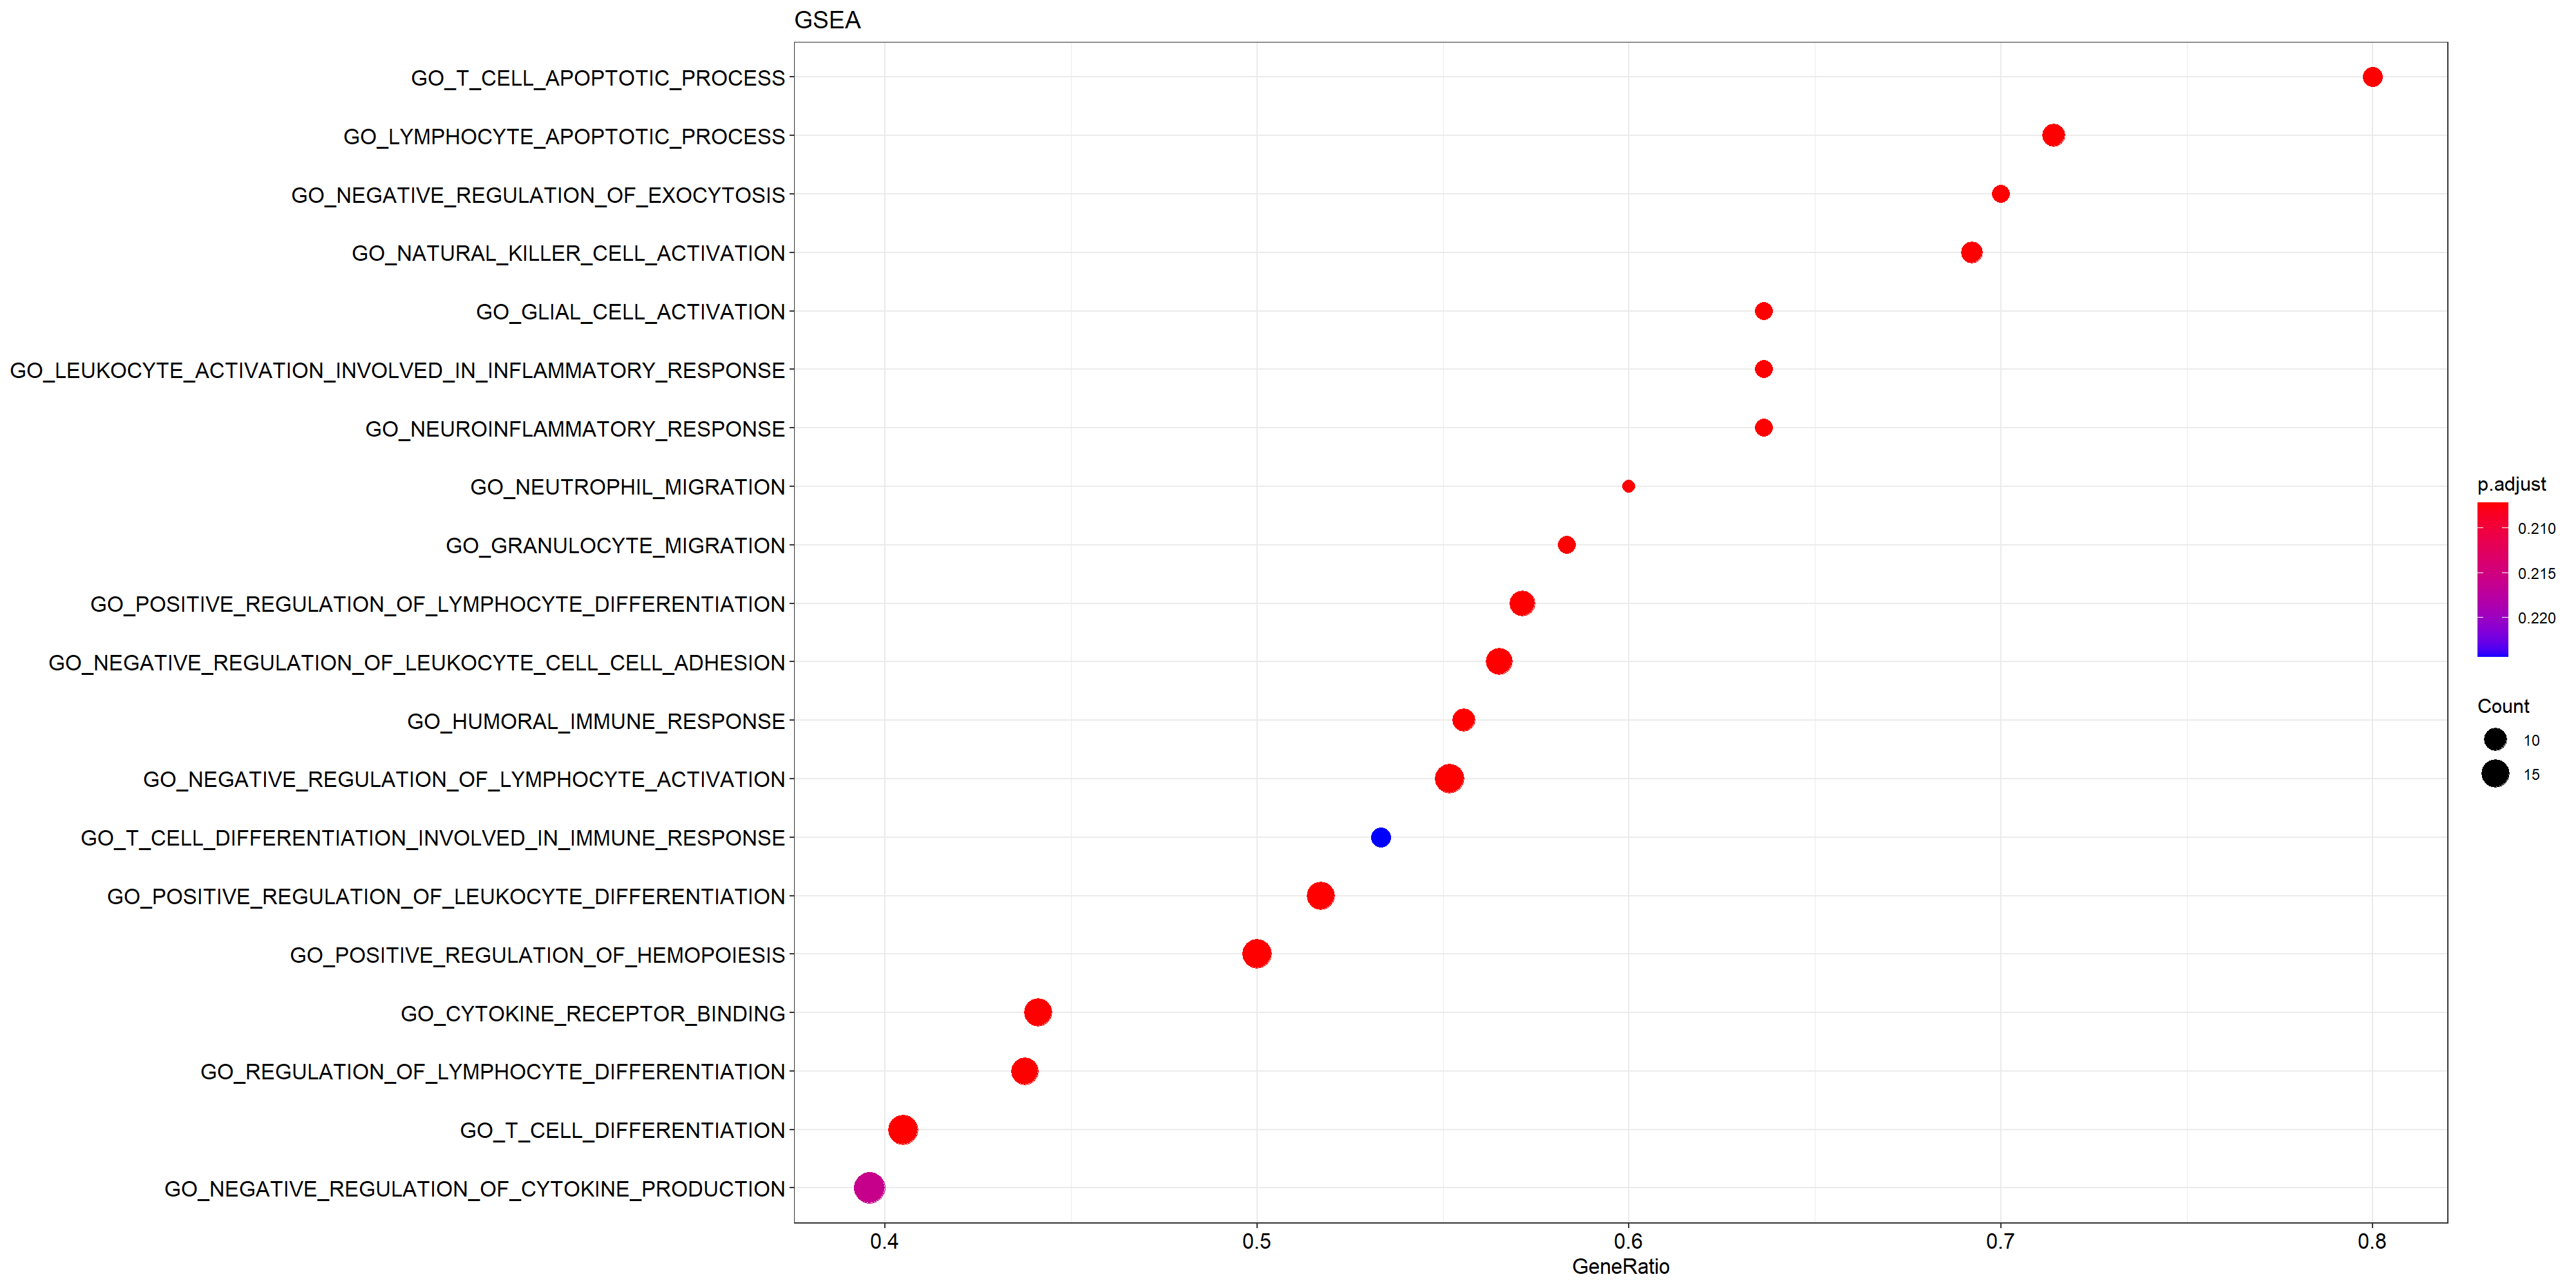
\includegraphics[width=5cm]{Figures/Path/CTLvs2_em_dotplot.png} }}%
\caption{Bar plot and dot plot visualization for over representation analysis and gene set enrichment analysis, respectively, of sutbype in Blood-HD-m.}
\label{fig:path-blood-m-sub}%
\end{figure}

\textbf{Pa-AD.} As it can be seen in the bar plots of Fig. \ref{fig:path-pa-ad}, the female and male datasets only have six equal pathways which are involved in synapse. The female results associate with synapse processes, neuron projection and differentiation, detoxification of inorganic compounds, and respiratory system development. Whereas the male set was related in the majority with synapse processes, transport, nervous system processes, and cognition, memory and adult behaviour; the latter pathway are truly interesting. Moreover, GSEA results of both sexes have many similarities (34/40); the difference resides on the male containing more cellular respiration pathways. According to GSEA, the female set is linked to cytosolic ribosome, synapse, electron transport chain, translation of proteins to membrane, axon, substantia nigra development, and node of Ranvier; the male counterpart was also related to node of Ranvier, substantia nigra development, synapse, translation of proteins, cytosolic ribosome, and axon.

\begin{figure}[!ht]%
    \centering
    \subfloat{{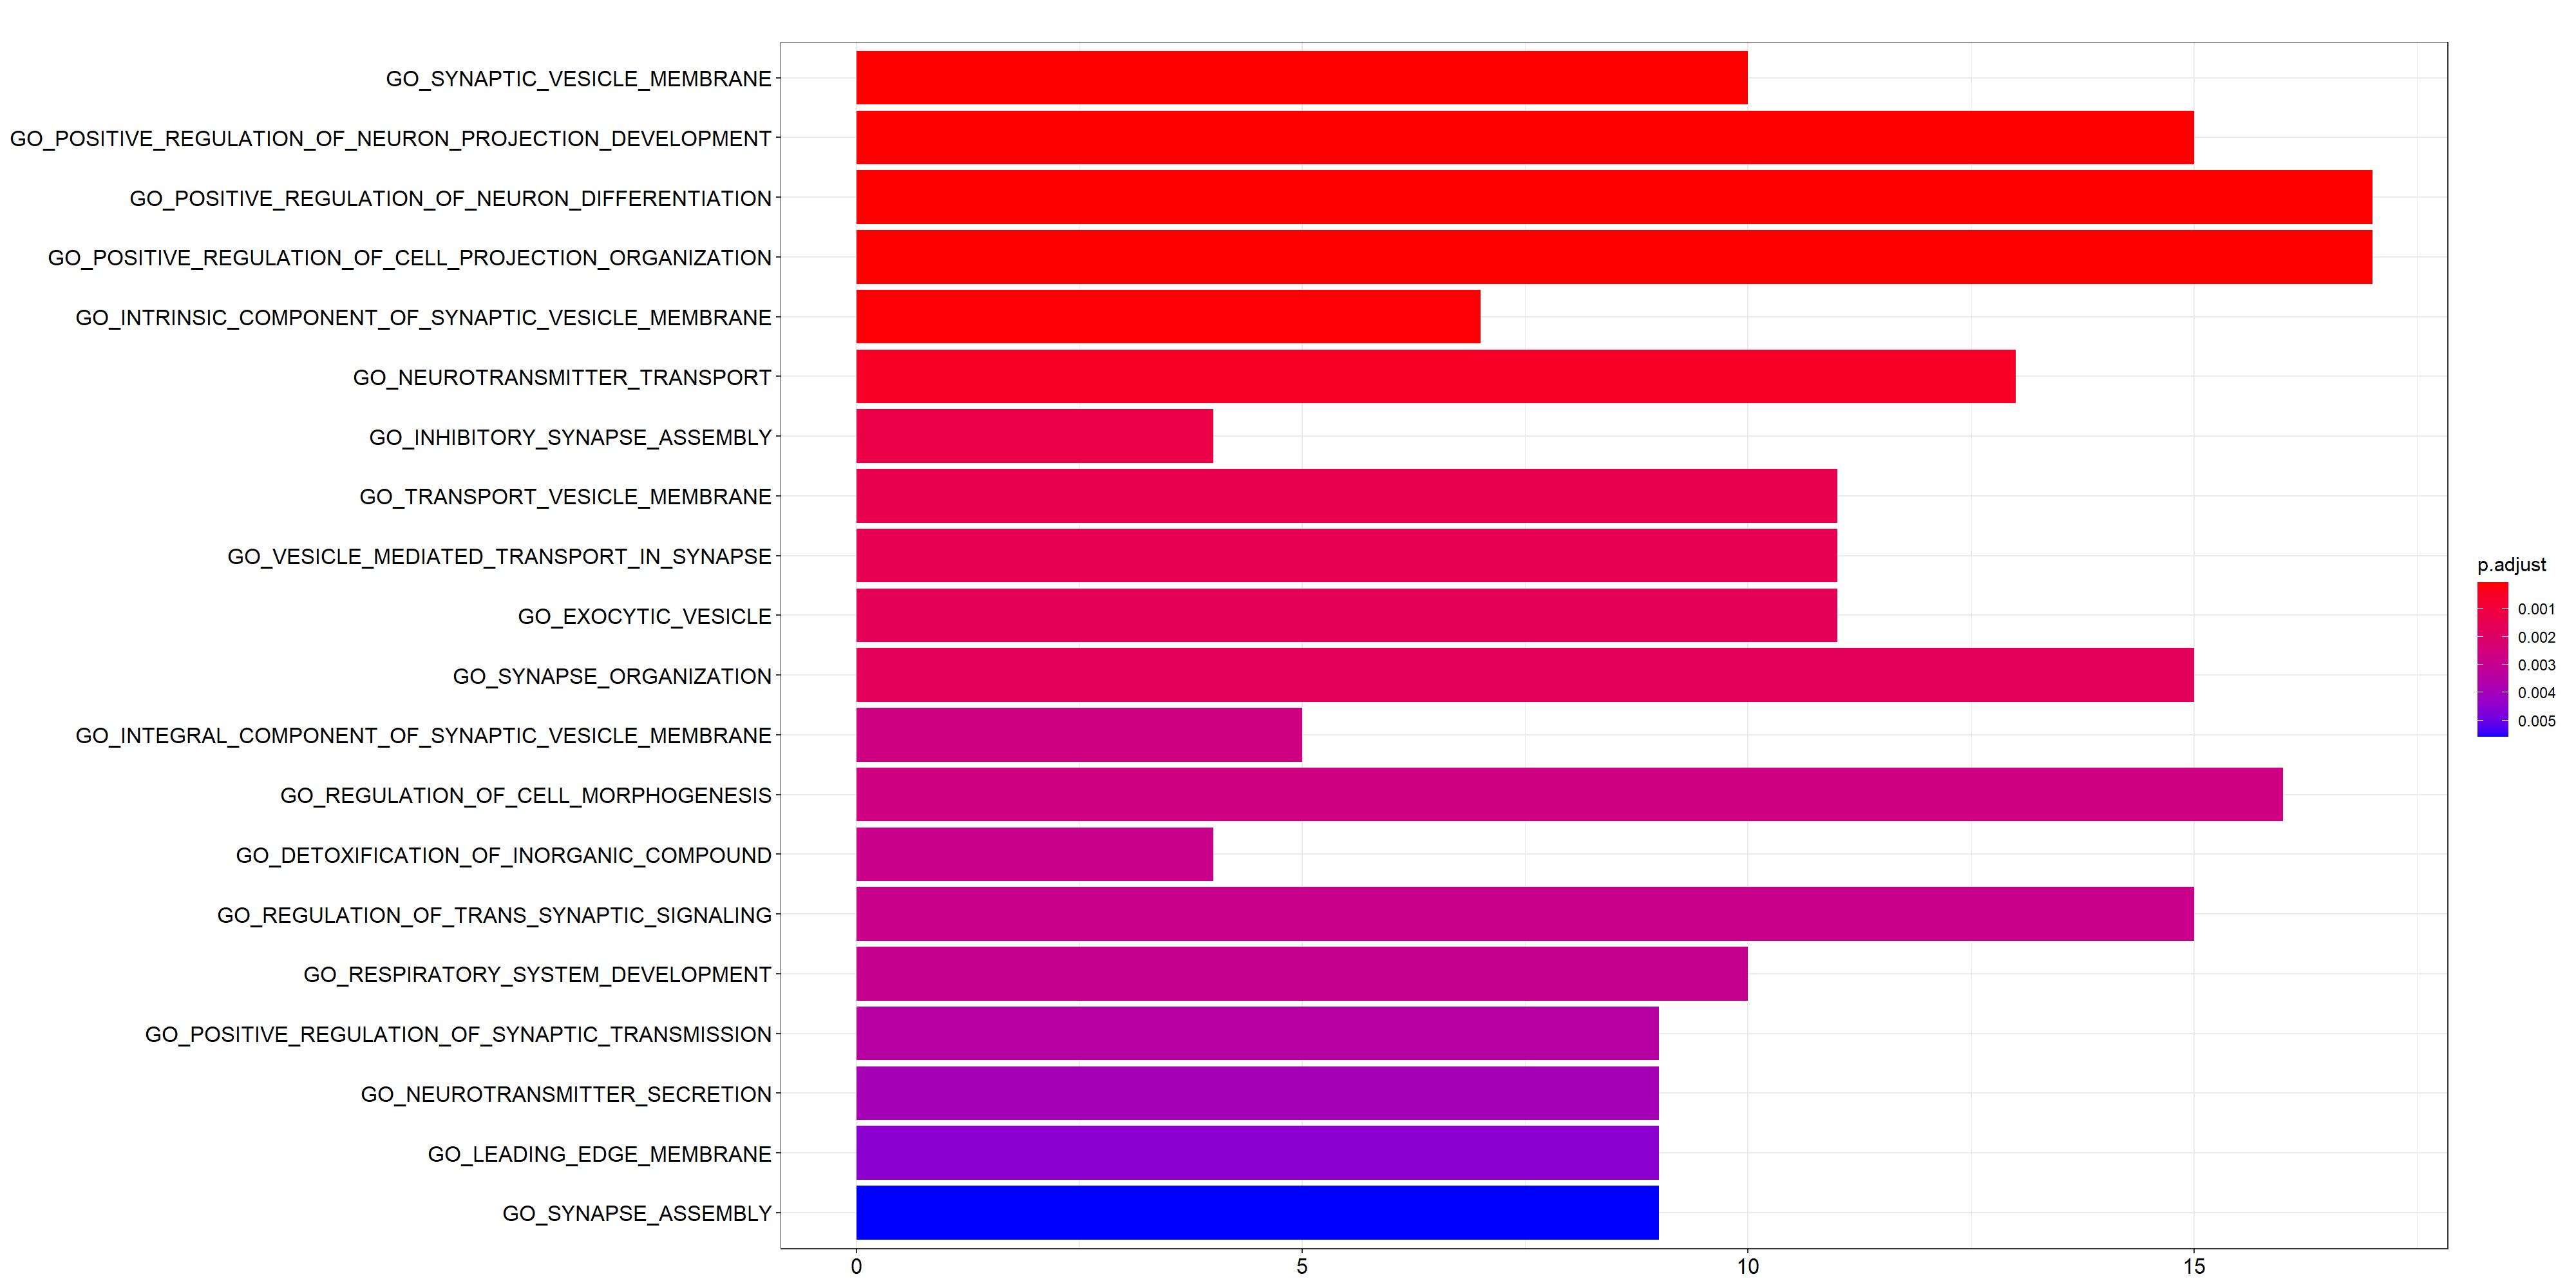
\includegraphics[width=5cm]{Figures/Path/CTLvsAD_ef_barplot-pa.png} }}%
    \qquad
    \subfloat{{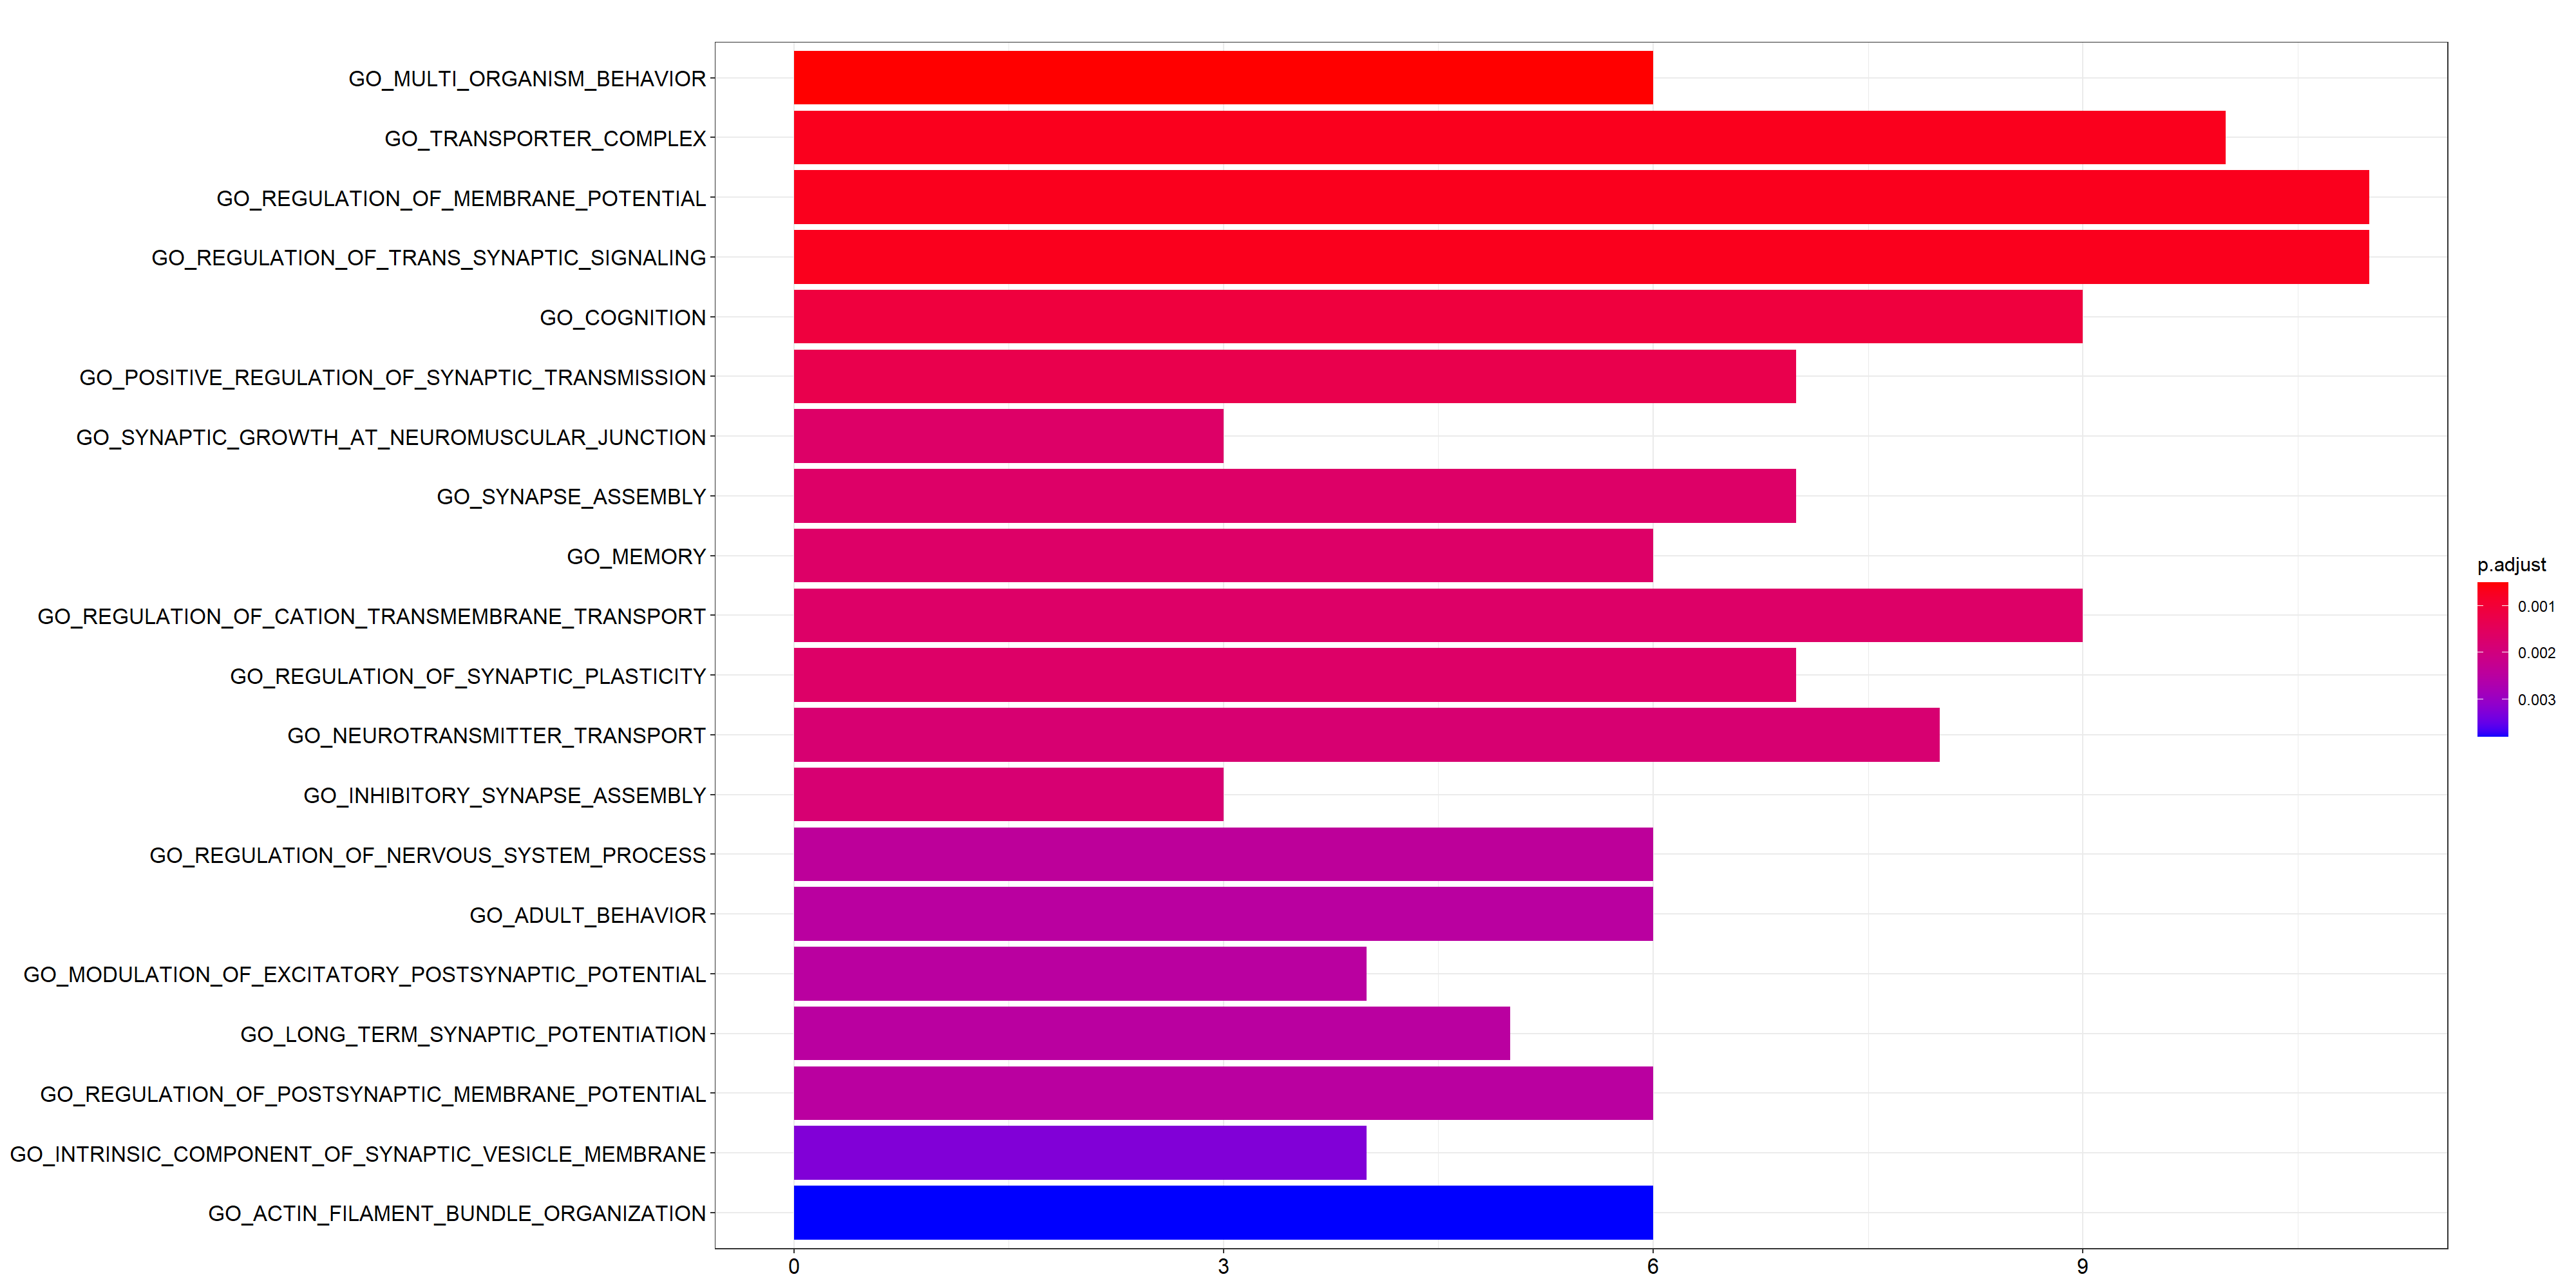
\includegraphics[width=5cm]{Figures/Path/CTLvsAD_em_barplot-pa.png} }}%
    \\
    \subfloat{{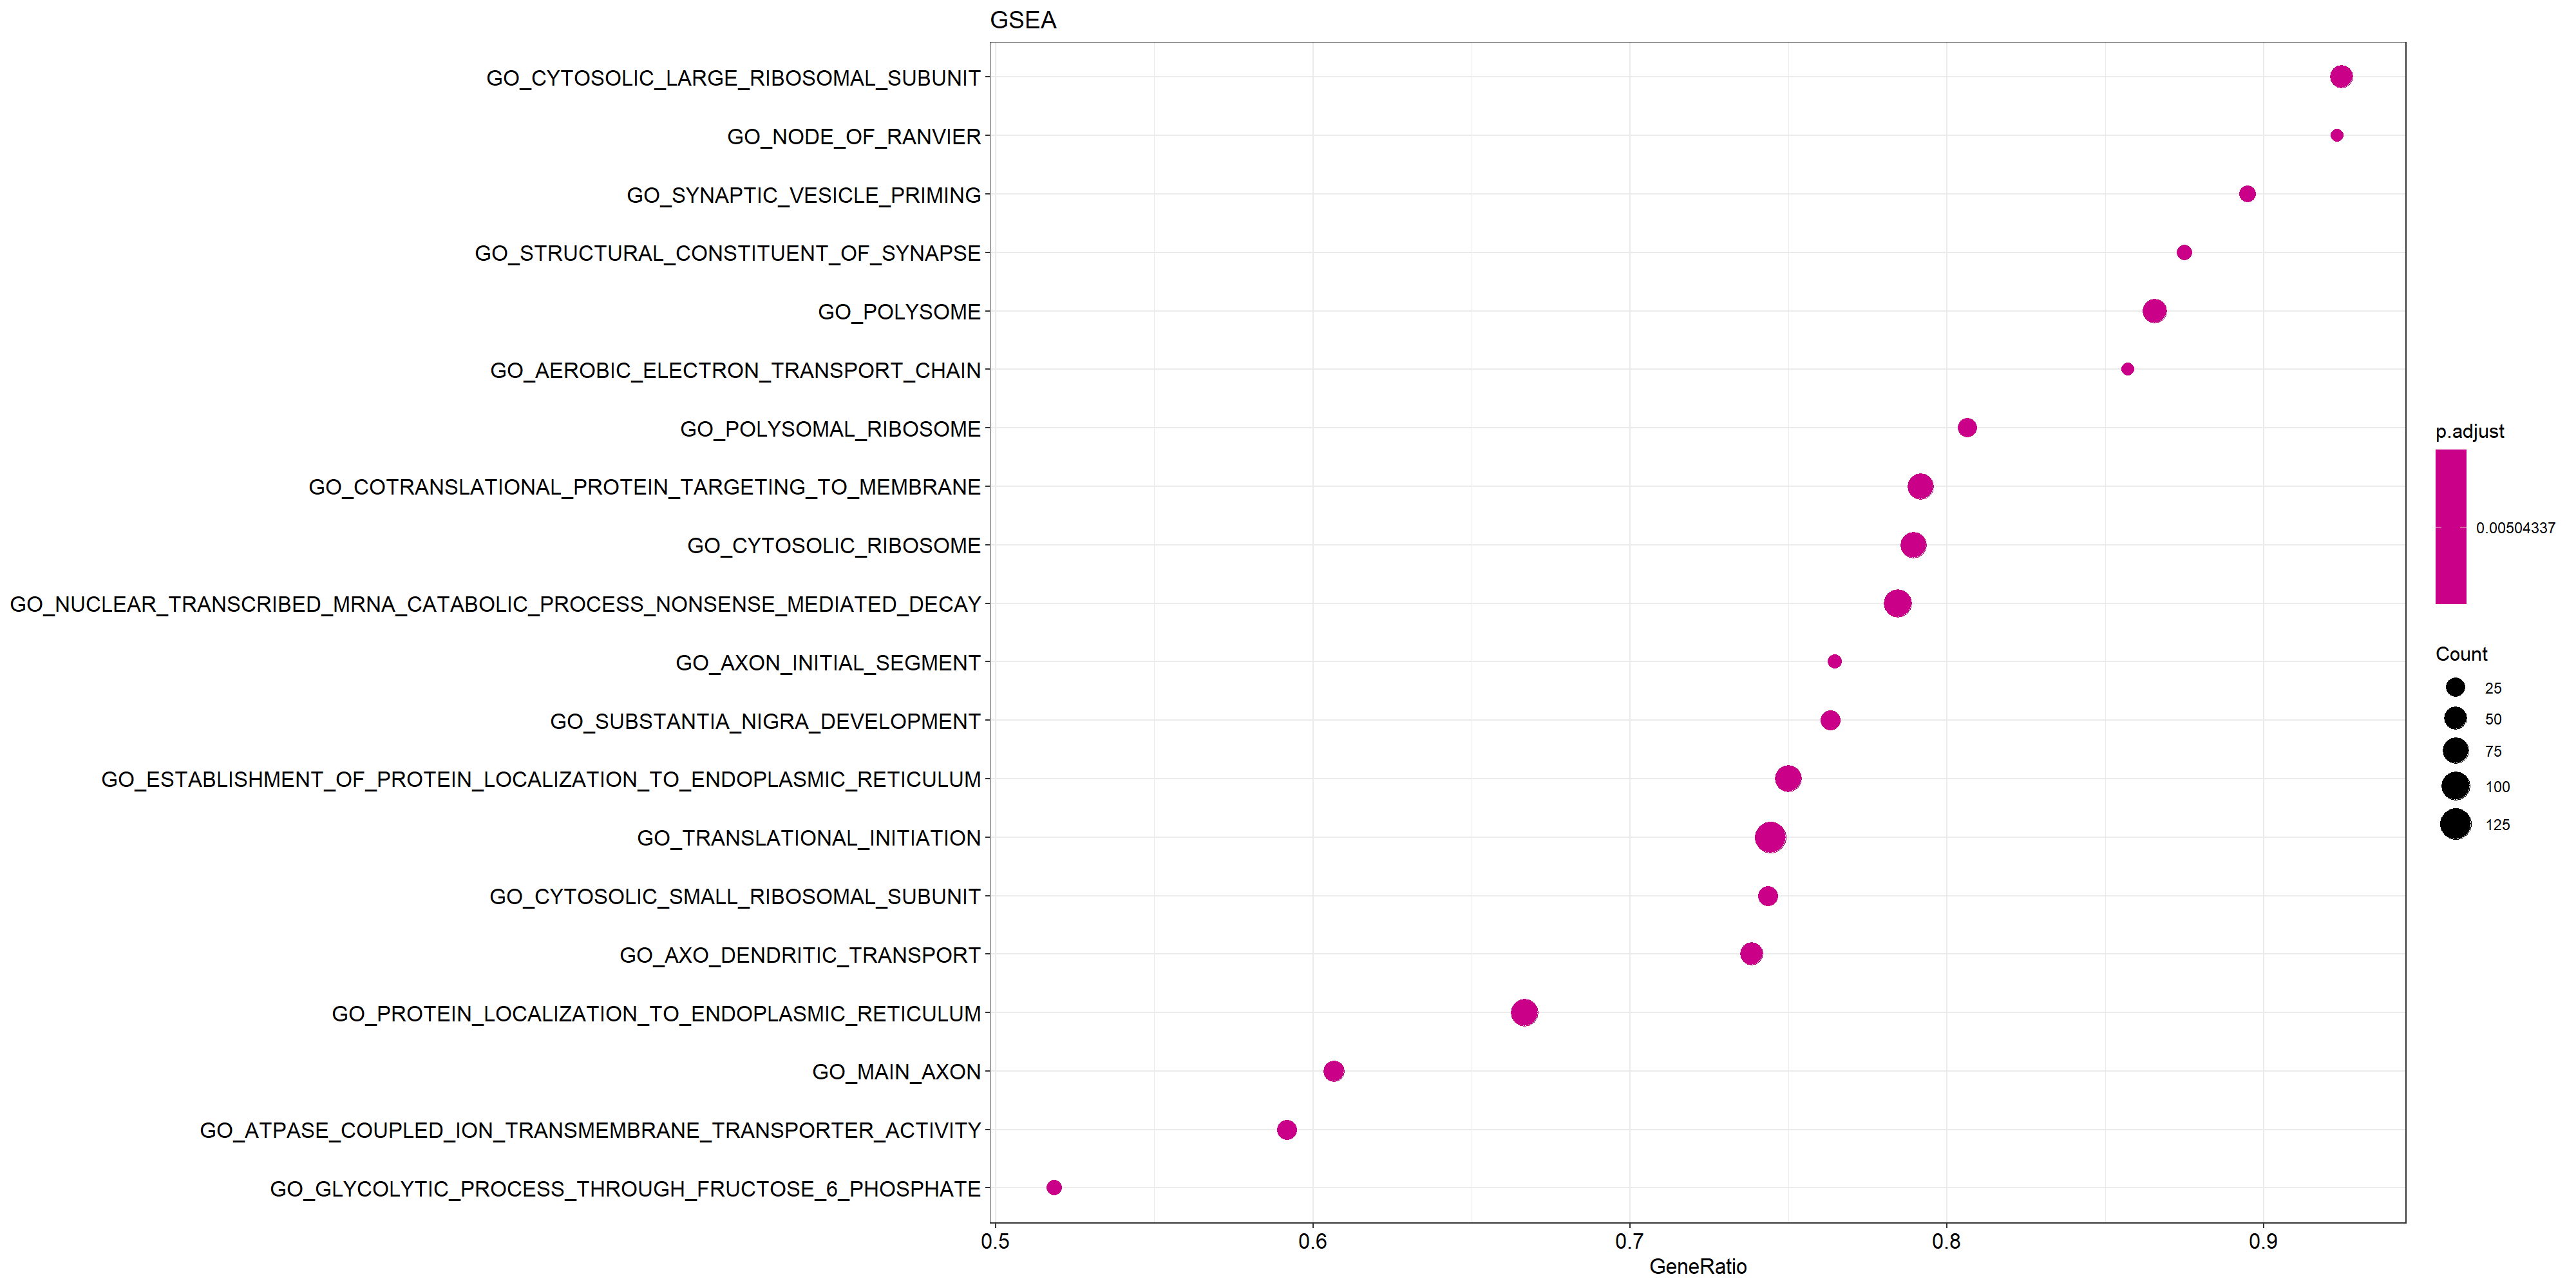
\includegraphics[width=5cm]{Figures/Path/CTLvsAD_ef_dotplot-pa.png} }}%
    \qquad
    \subfloat{{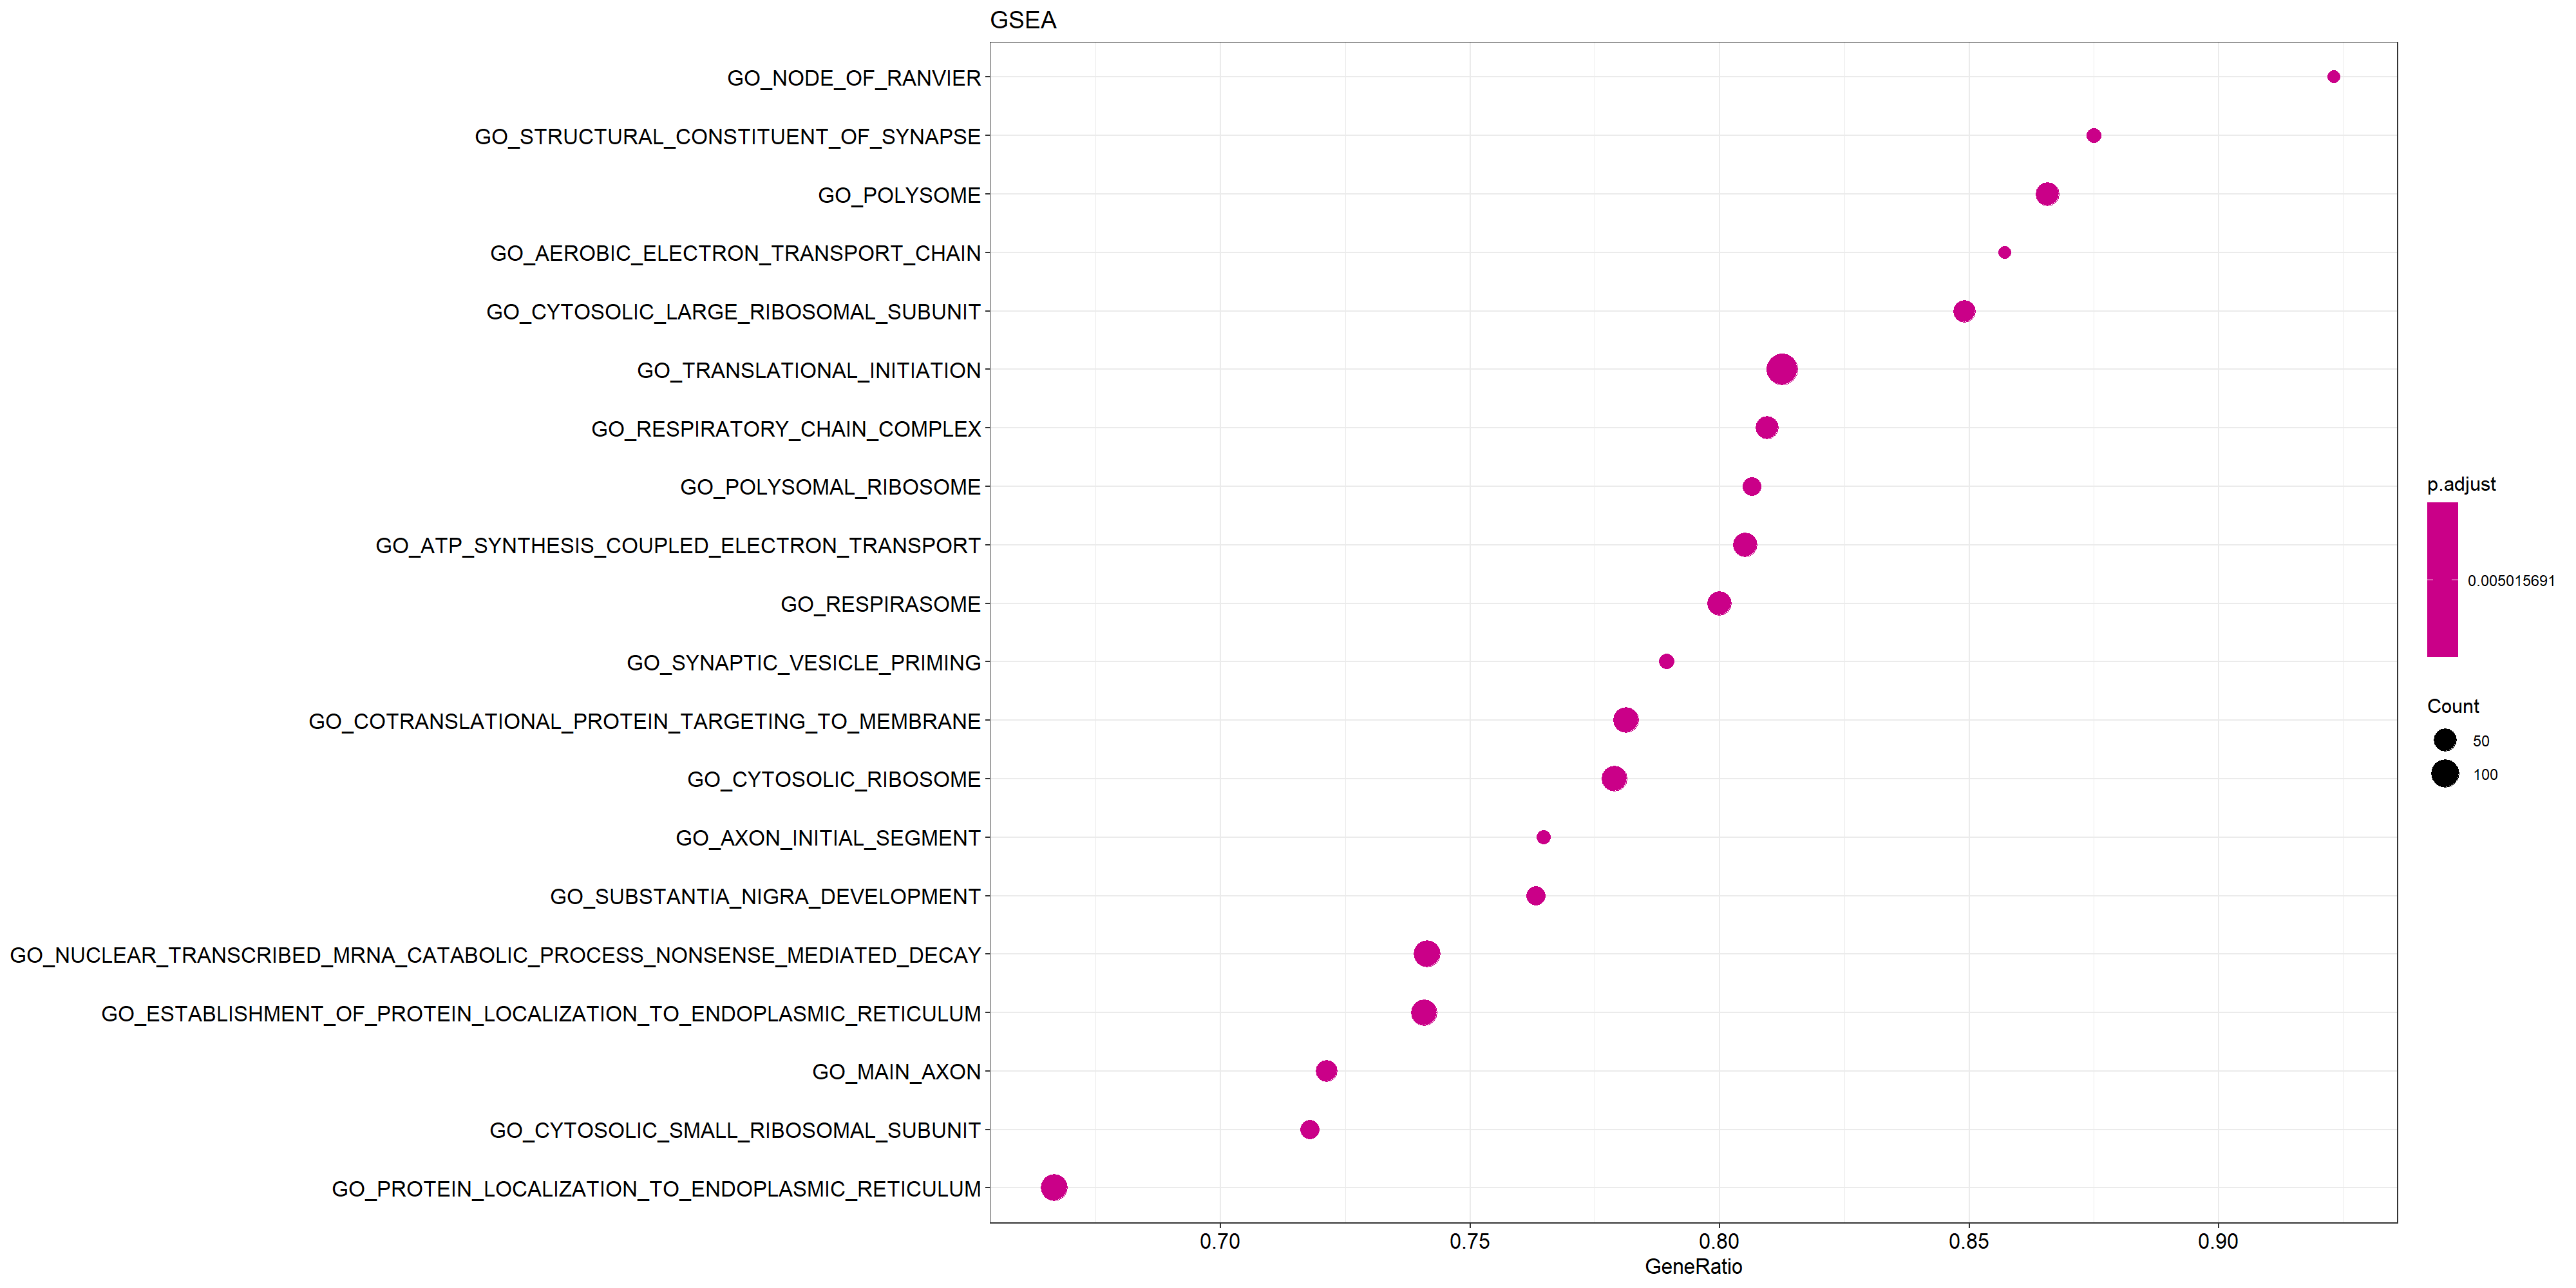
\includegraphics[width=5cm]{Figures/Path/CTLvsAD_em_dotplot-pa.png} }}%
\caption{Bar plot and dot plot visualization for over representation analysis and gene set enrichment analysis, respectively, of Pa-AD.}
\footnotesize Left for female; right for male.
\label{fig:path-pa-ad}%
\end{figure}

Using the DEGs intercepts, the pathways enriched for each sex can be obtained, refer to Appendix \ref{paths-comparison}. For the down-regulated genes, the intercepting routes are binding and junction, postsynapse and synapse, and cytoskeleton organization. The exclusive male pathways are related to abnormality of bone mineral density, abnormality of frontal sinuses, and cell junction assembly. The unique paths of the female DEGs are associated with retinal arterial tortuosity, mitochondrial respiratory chain defects, action tremor, and polyneuropathy. Furthermore, the results for the intersection of over-expressed genes are related to synapse, secretion, cell-cell signaling, and neuron projection. The female pathways are synapse, neuron projection, poor speech, abnormality in forehead and palpebral fissure, and muscle weakness. The male set just had four genes, so no ORA could be performed and each gene was researched. CRHBP is involved in presynaptic functions. PCP4 is related to neuron differentiation. MET is an oncogene which is linked to the RET pathway. Lastly, OPACIN increases myelin expression and promotes oligodendrocyte differentiation.

\textbf{Temp-AD.} In contrast to other datasets, the ORA results of both sexes are very related with brain processes. The female set is associated with semaphorin activity (axon guidance molecules), synapse, glia cell differentiation and nervous system development, and epithelial tube morphogenesis and branching. The male counterpart is linked to synapse and neurotransmitters, exocytosis by syntaxin, and neuron projection pathways. Nonetheless, the over represented routes of female and male shown in Fig. \ref{fig:path-temp-ad} only overlap in three paths. On the other hand, the GSEA pathways between the sexes are almost the same (36/40). 

\begin{figure}[!ht]%
    \centering
    \subfloat{{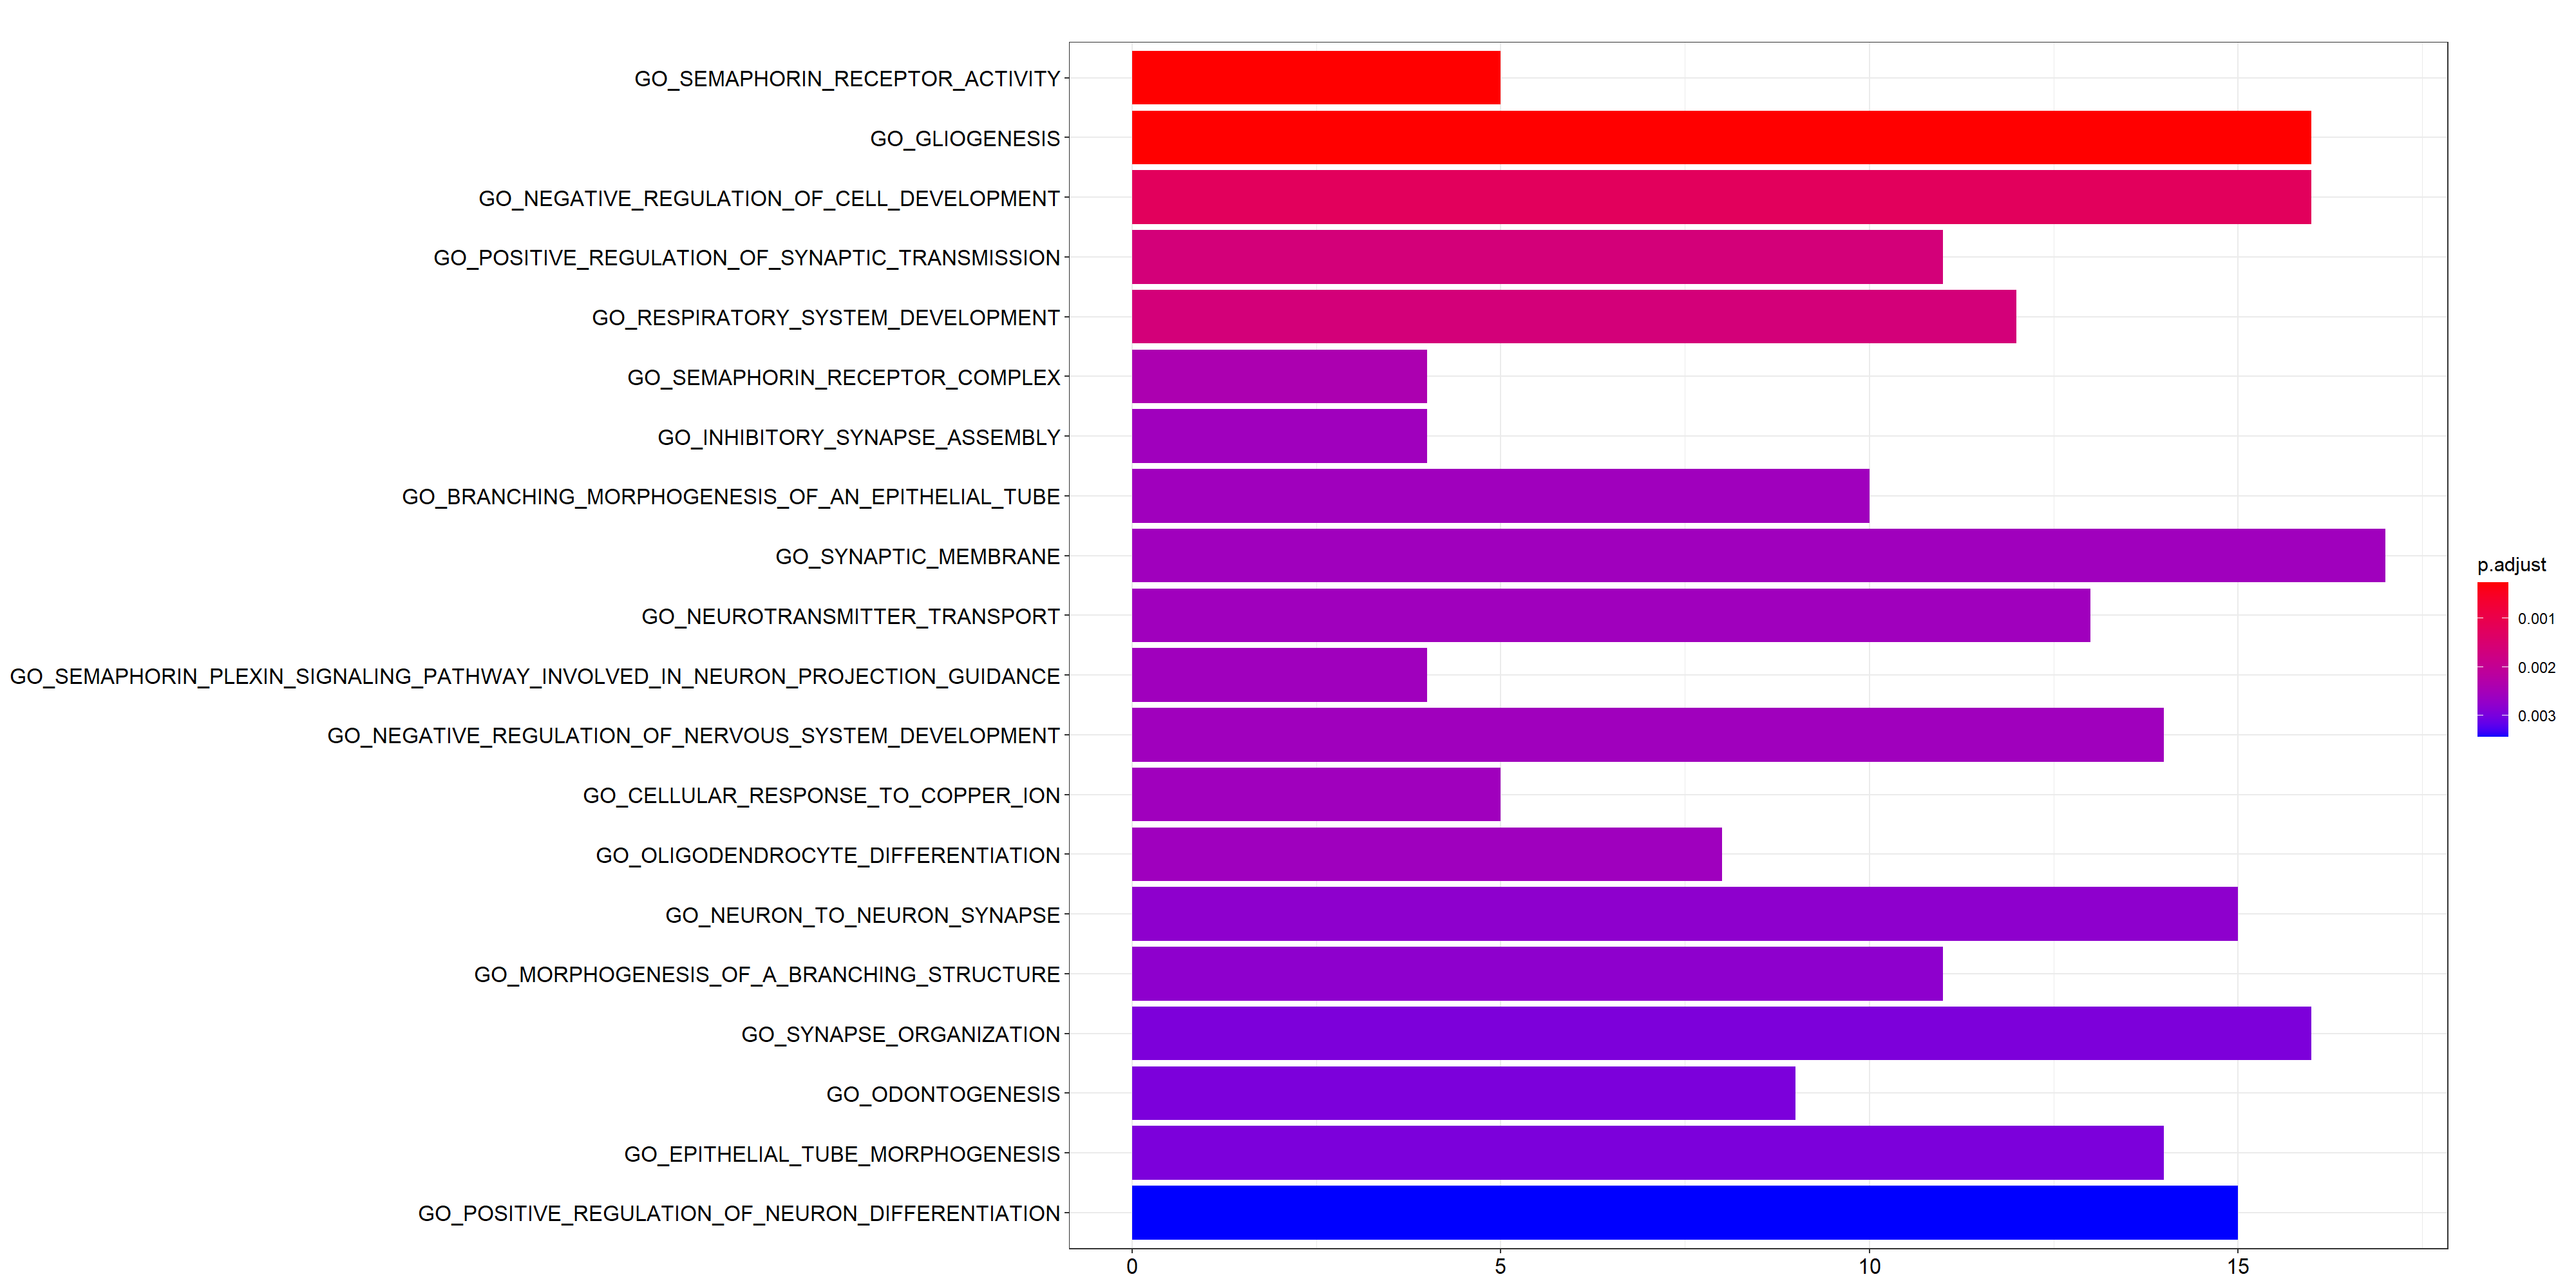
\includegraphics[width=5cm]{Figures/Path/CTLvsAD_ef_barplot.png} }}%
    \qquad
    \subfloat{{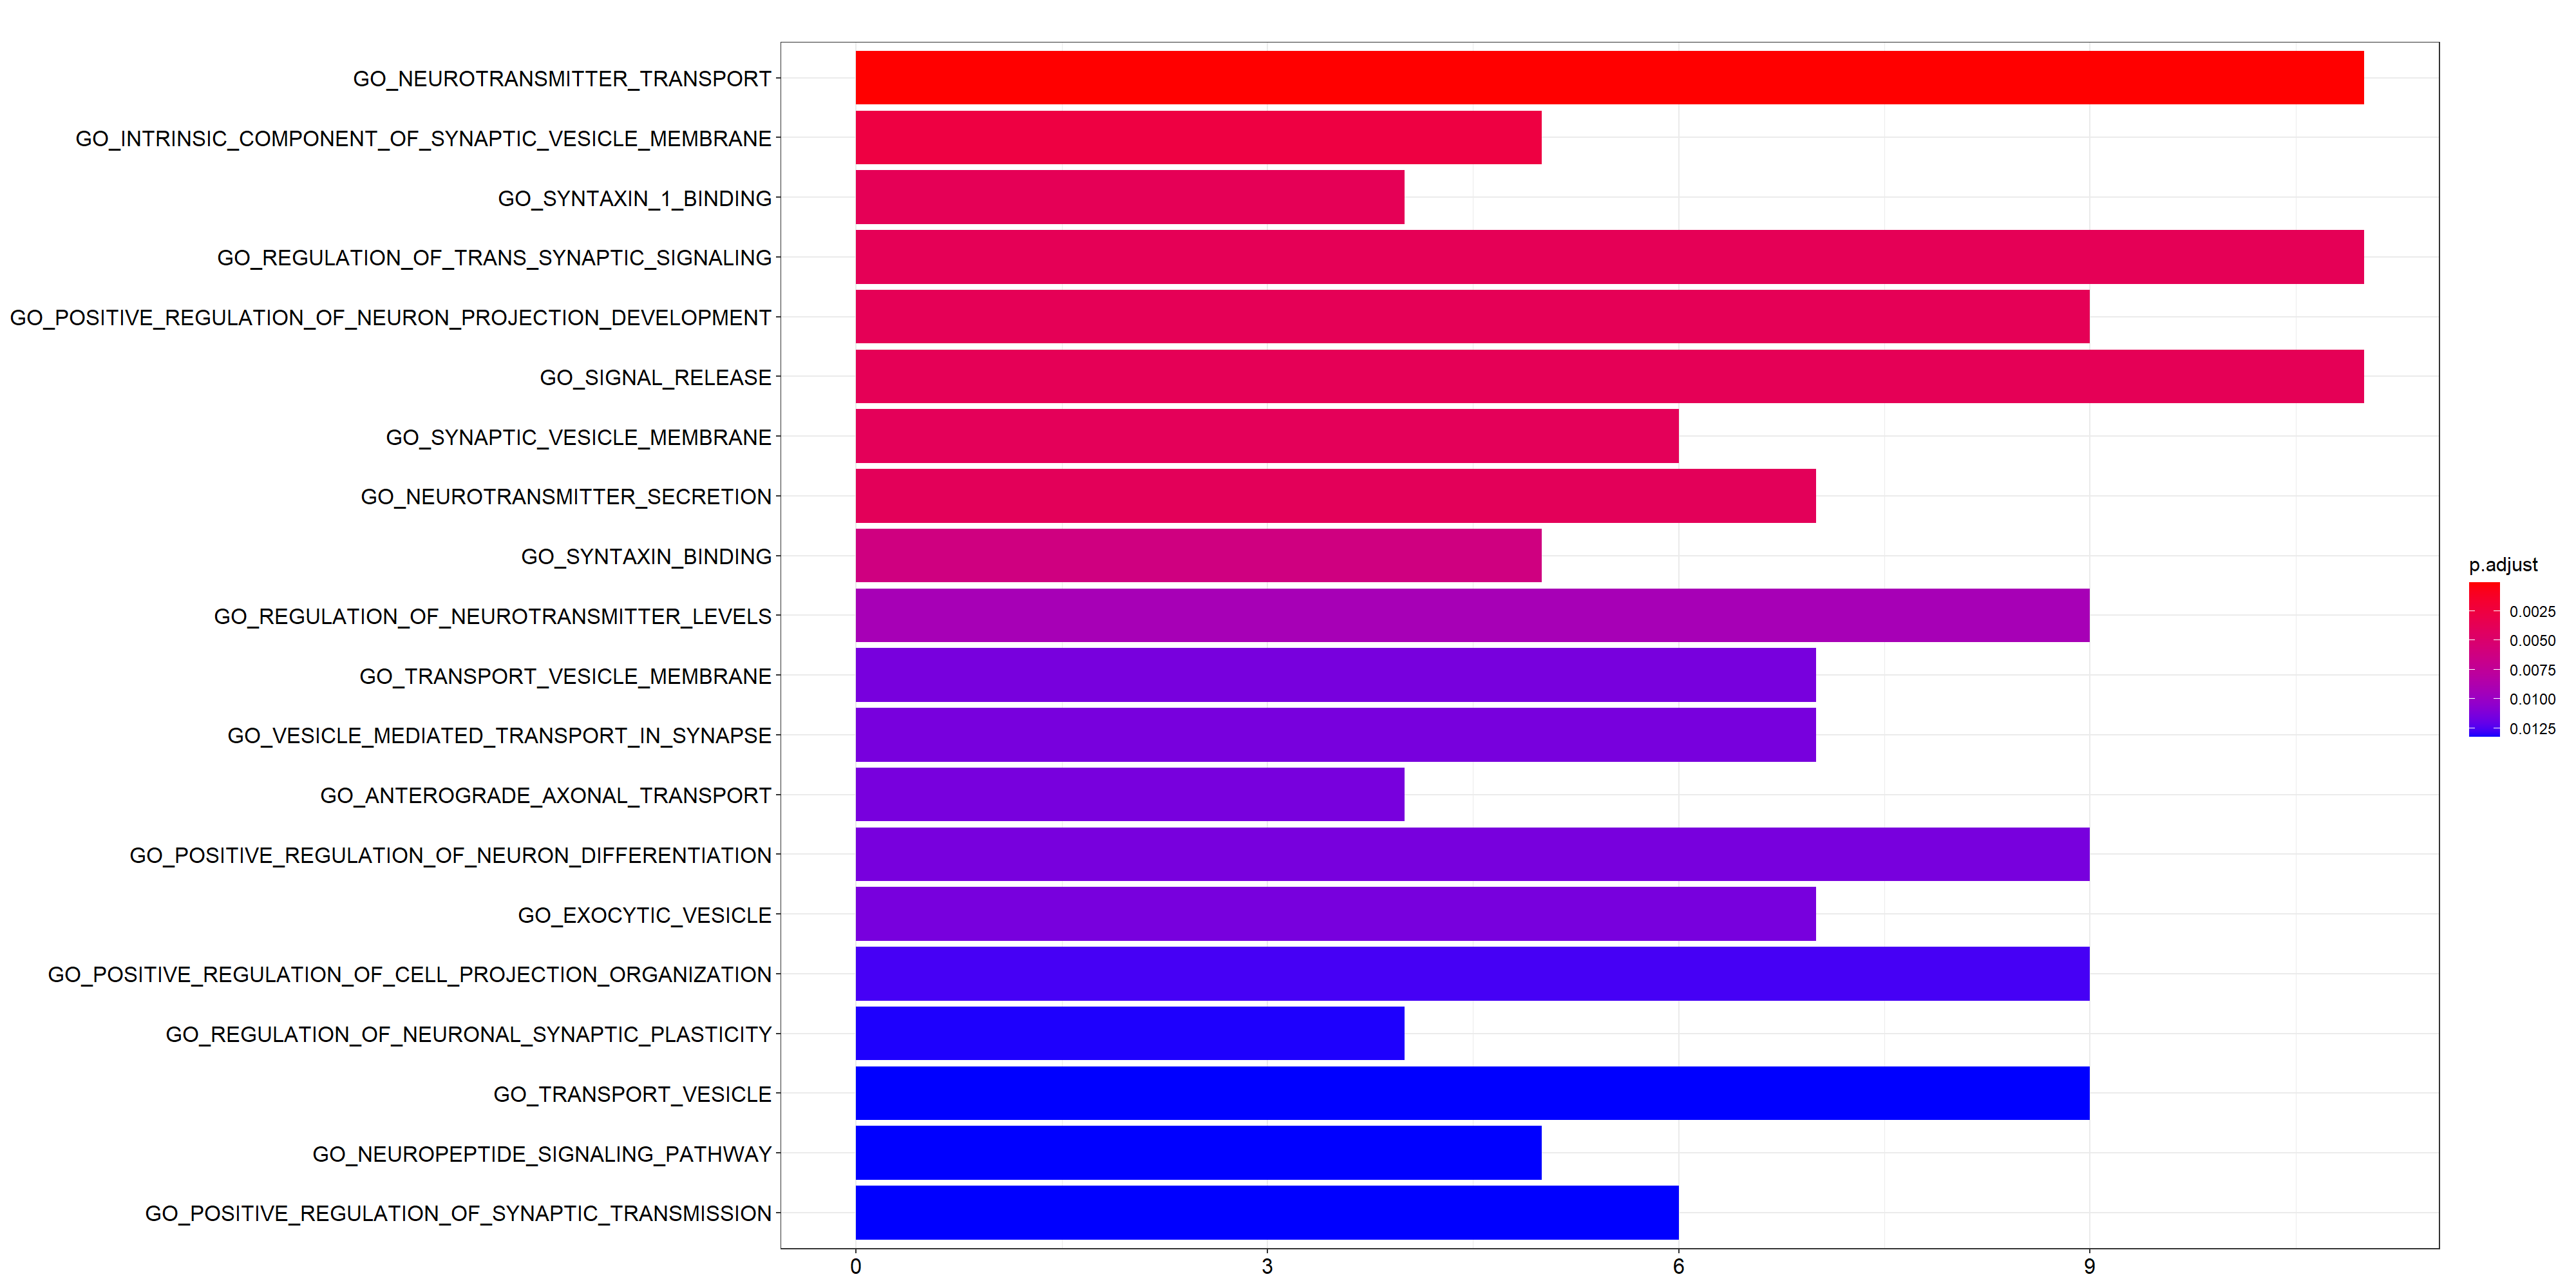
\includegraphics[width=5cm]{Figures/Path/CTLvsAD_em_barplot.png} }}%
    \\
    \subfloat{{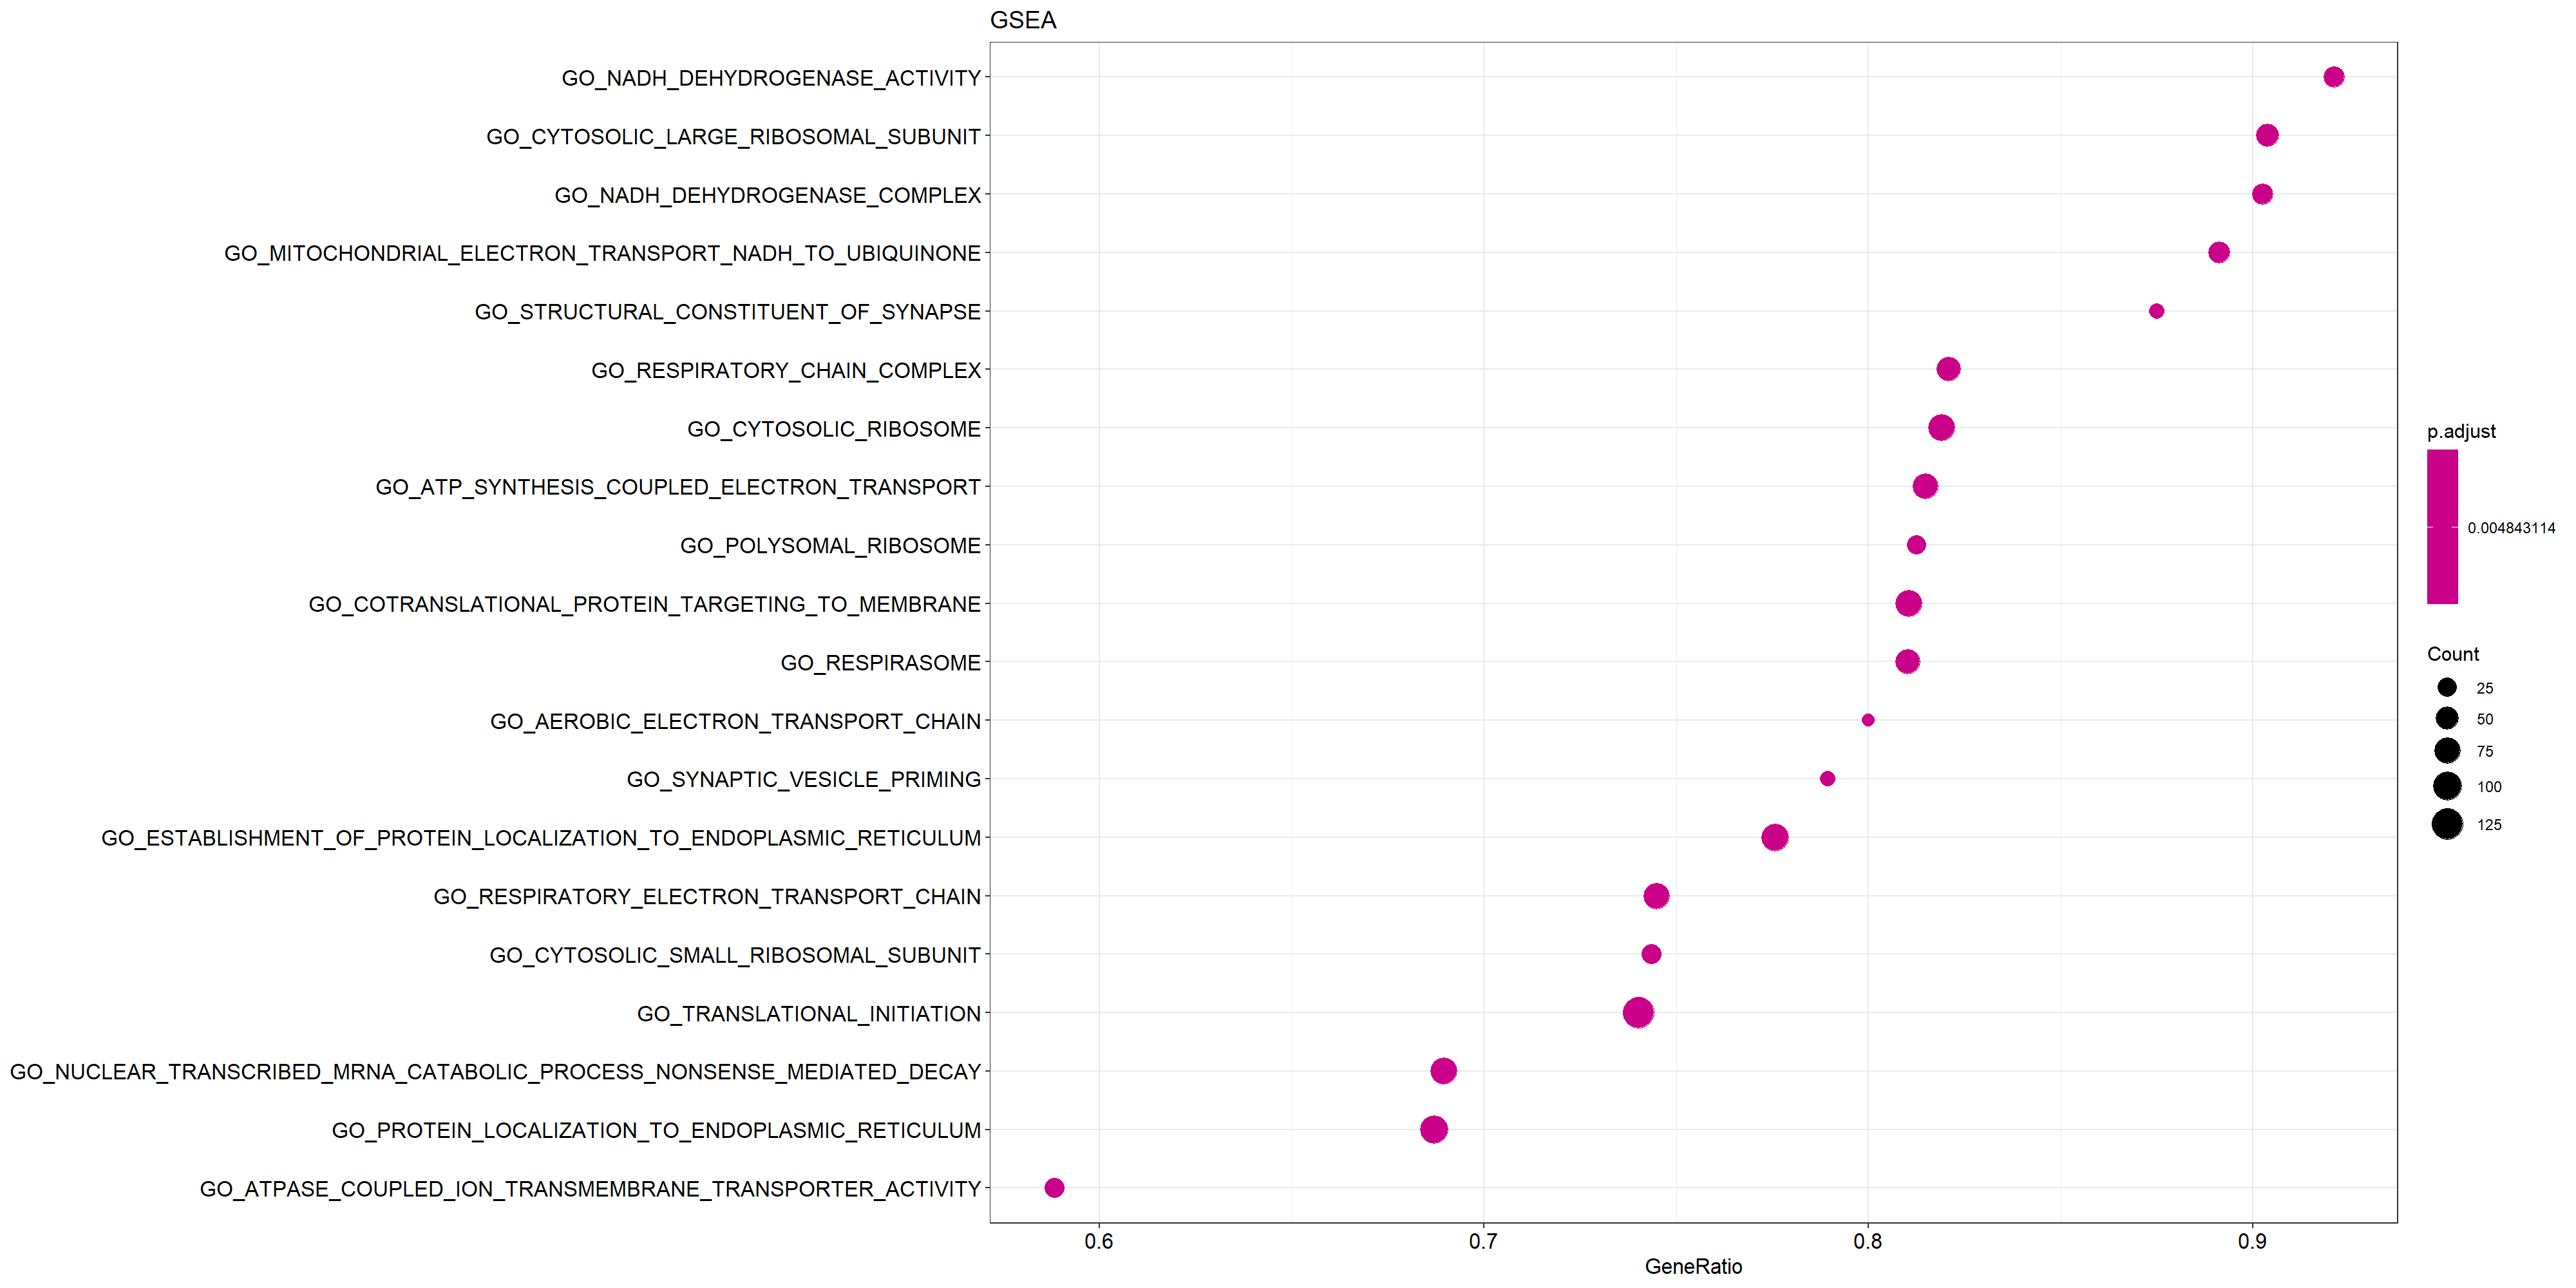
\includegraphics[width=5cm]{Figures/Path/CTLvsAD_ef_dotplot.png} }}%
    \qquad
    \subfloat{{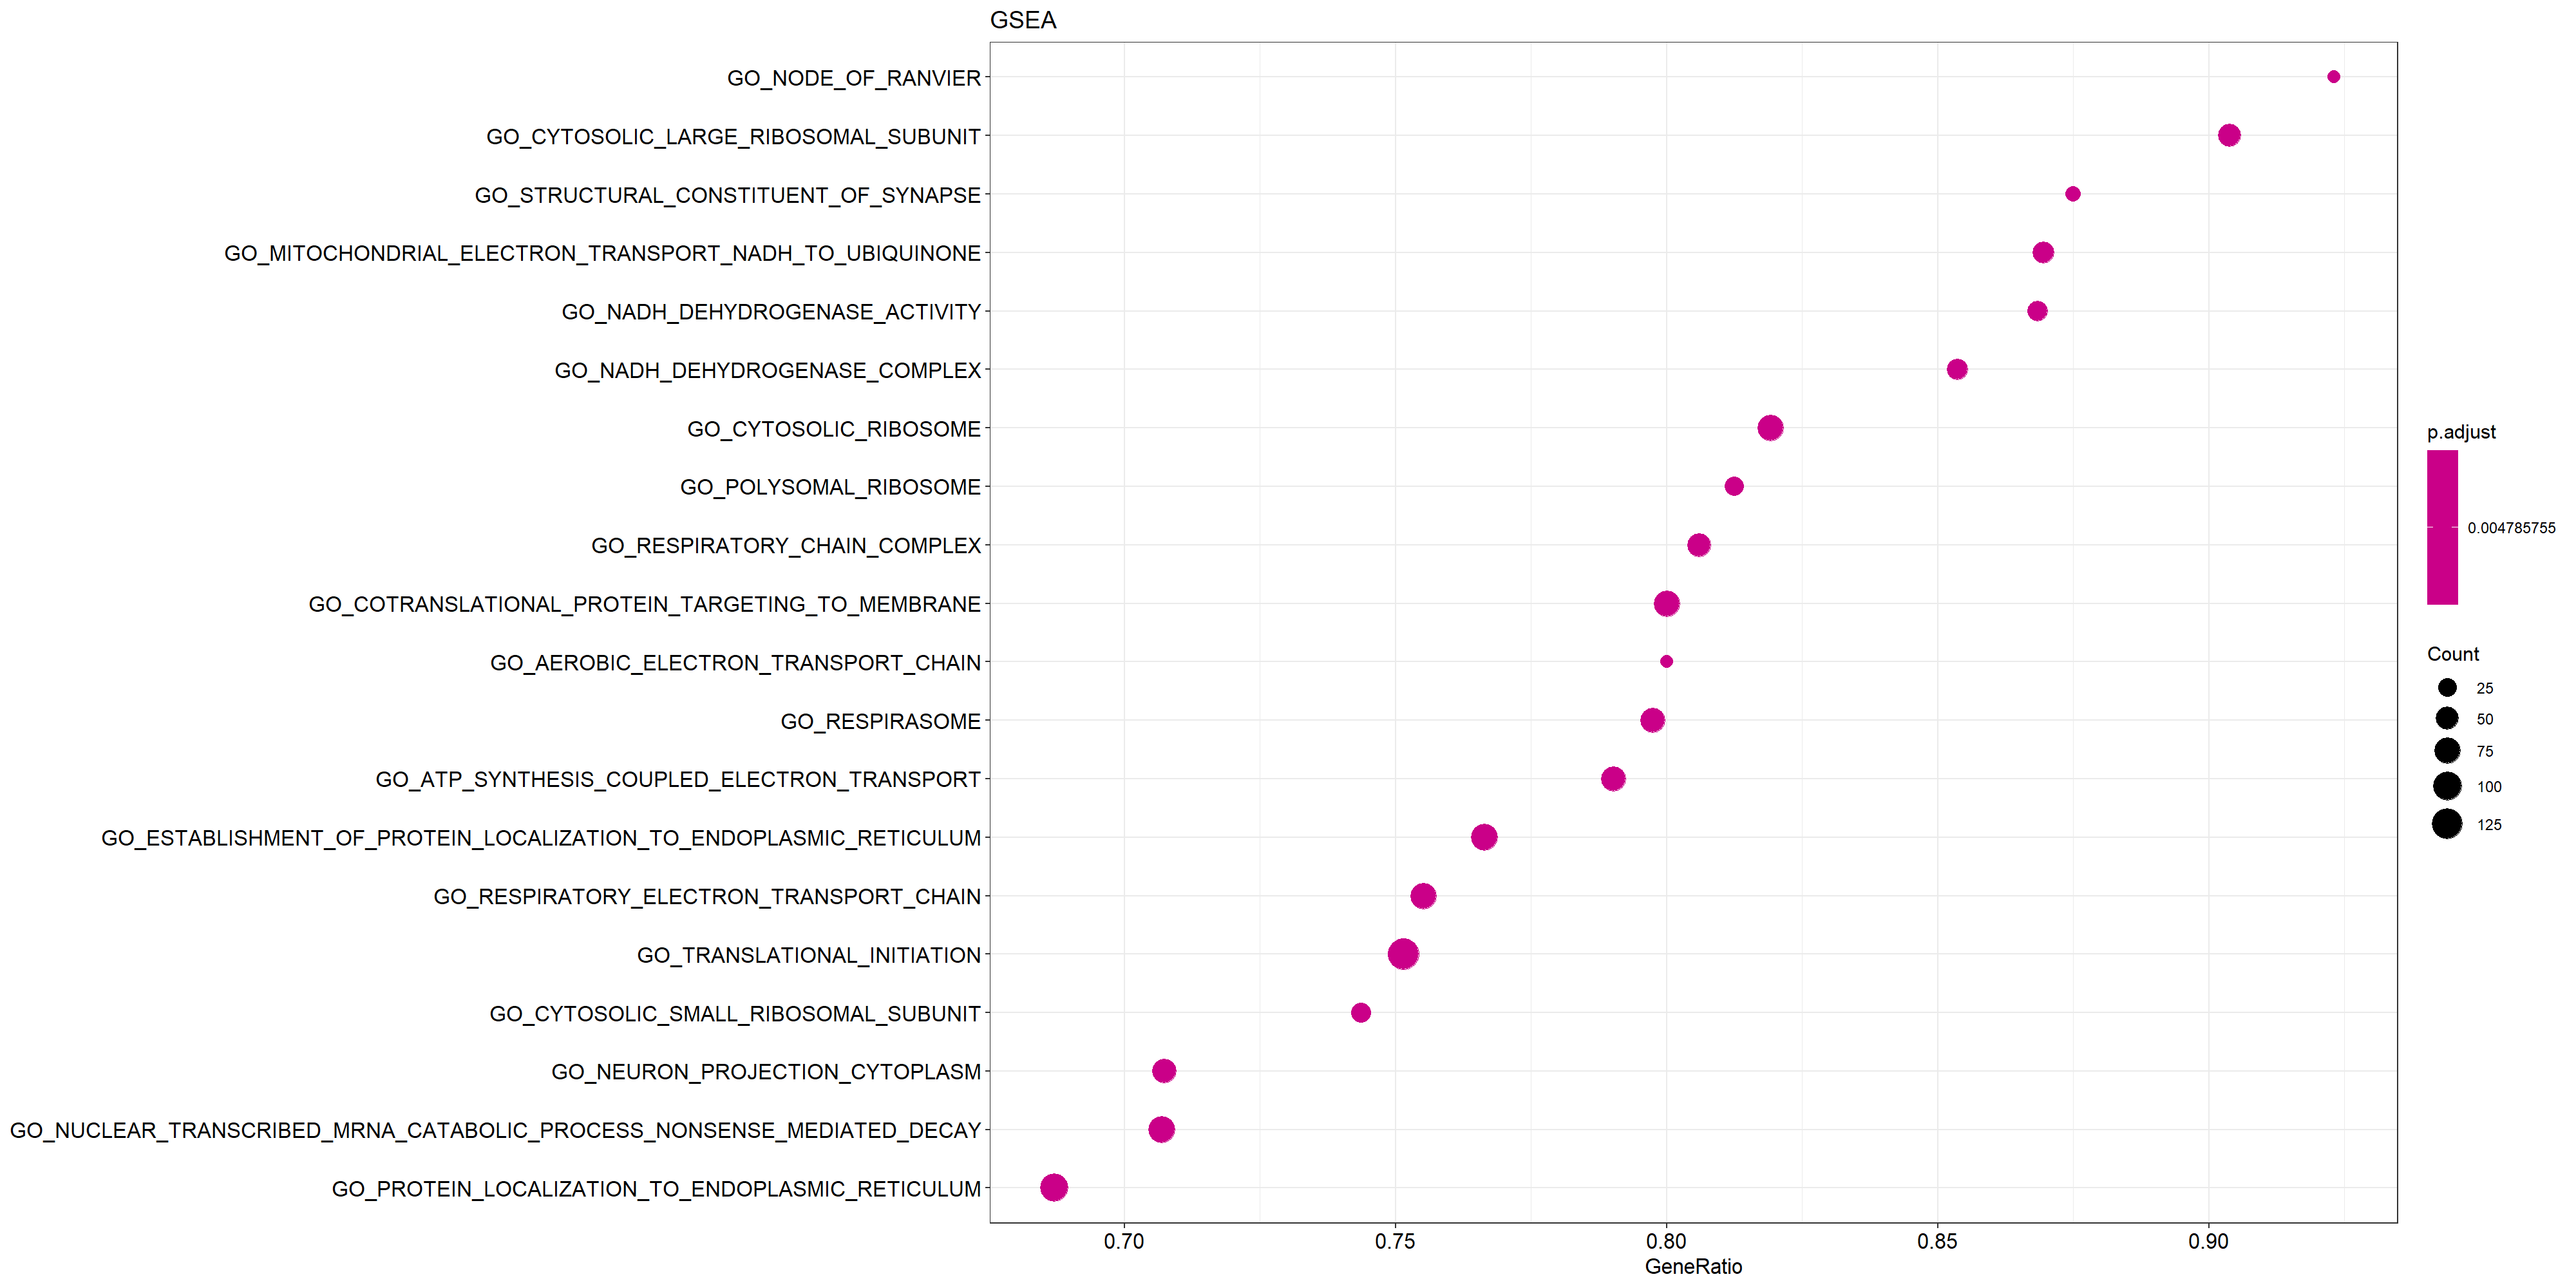
\includegraphics[width=5cm]{Figures/Path/CTLvsAD_em_dotplot.png} }}%
\caption{Bar plot and dot plot visualization for over representation analysis and gene set enrichment analysis, respectively, of Temp-AD.}
\footnotesize Left for female; right for male.
\label{fig:path-temp-ad}%
\end{figure}

Using the intercepted and unique DEGs of Section \ref{res-dgea}, the exclusively and common pathways can be consulted. For the over-expressed genes, the intercepted pathways between sexes are related to synapse, cell-cell signaling and neuropeptides, neuron projection, and behaviour. The unique female pathways are GABA receptor, synapse by histamine, and neuron projection as well. For the male set, the associated pathways were neuron differentiation and axogenesis. Additionally, for the under-expressed genes, the common pathways are cell junction and actin binding, biological adhesion, abnormal peripheral nervous system morphology, and chronic axonal neuropathy. Then again, the female pathways are gliogenesis and neurogenesis, glia and neuron differentiation, biological adhesion, central nervous system development, and head development. The glomerular epithelial cell pathway was the only unique male route. See Appendix \ref{paths-comparison}.

\textbf{Hip-AD.} As seen in the information given in Fig. \ref{fig:path-hip-ad}, the over represented pathways among the male and female sets are divergent, just four routes are in common. However, the results from GSEA contains exactly the same paths; which are related to electron transport chain and cellular respiration, cytosolic ribosome, proton localization and transport, and substantia nigra development. On the other hand, the male bar plot is summarized in exocytosis by sintaxin, synapse and neurotransmitter, inclusion body assembly, long-term memory, and memory. The female results are involved in synapse and neurotransmitter, and memory as well, clathrin coated vesicles, ion channels, and dicarboxylic acid and $\alpha$ amino acid catabolic process.

\begin{figure}[!ht]%
    \centering
    \subfloat{{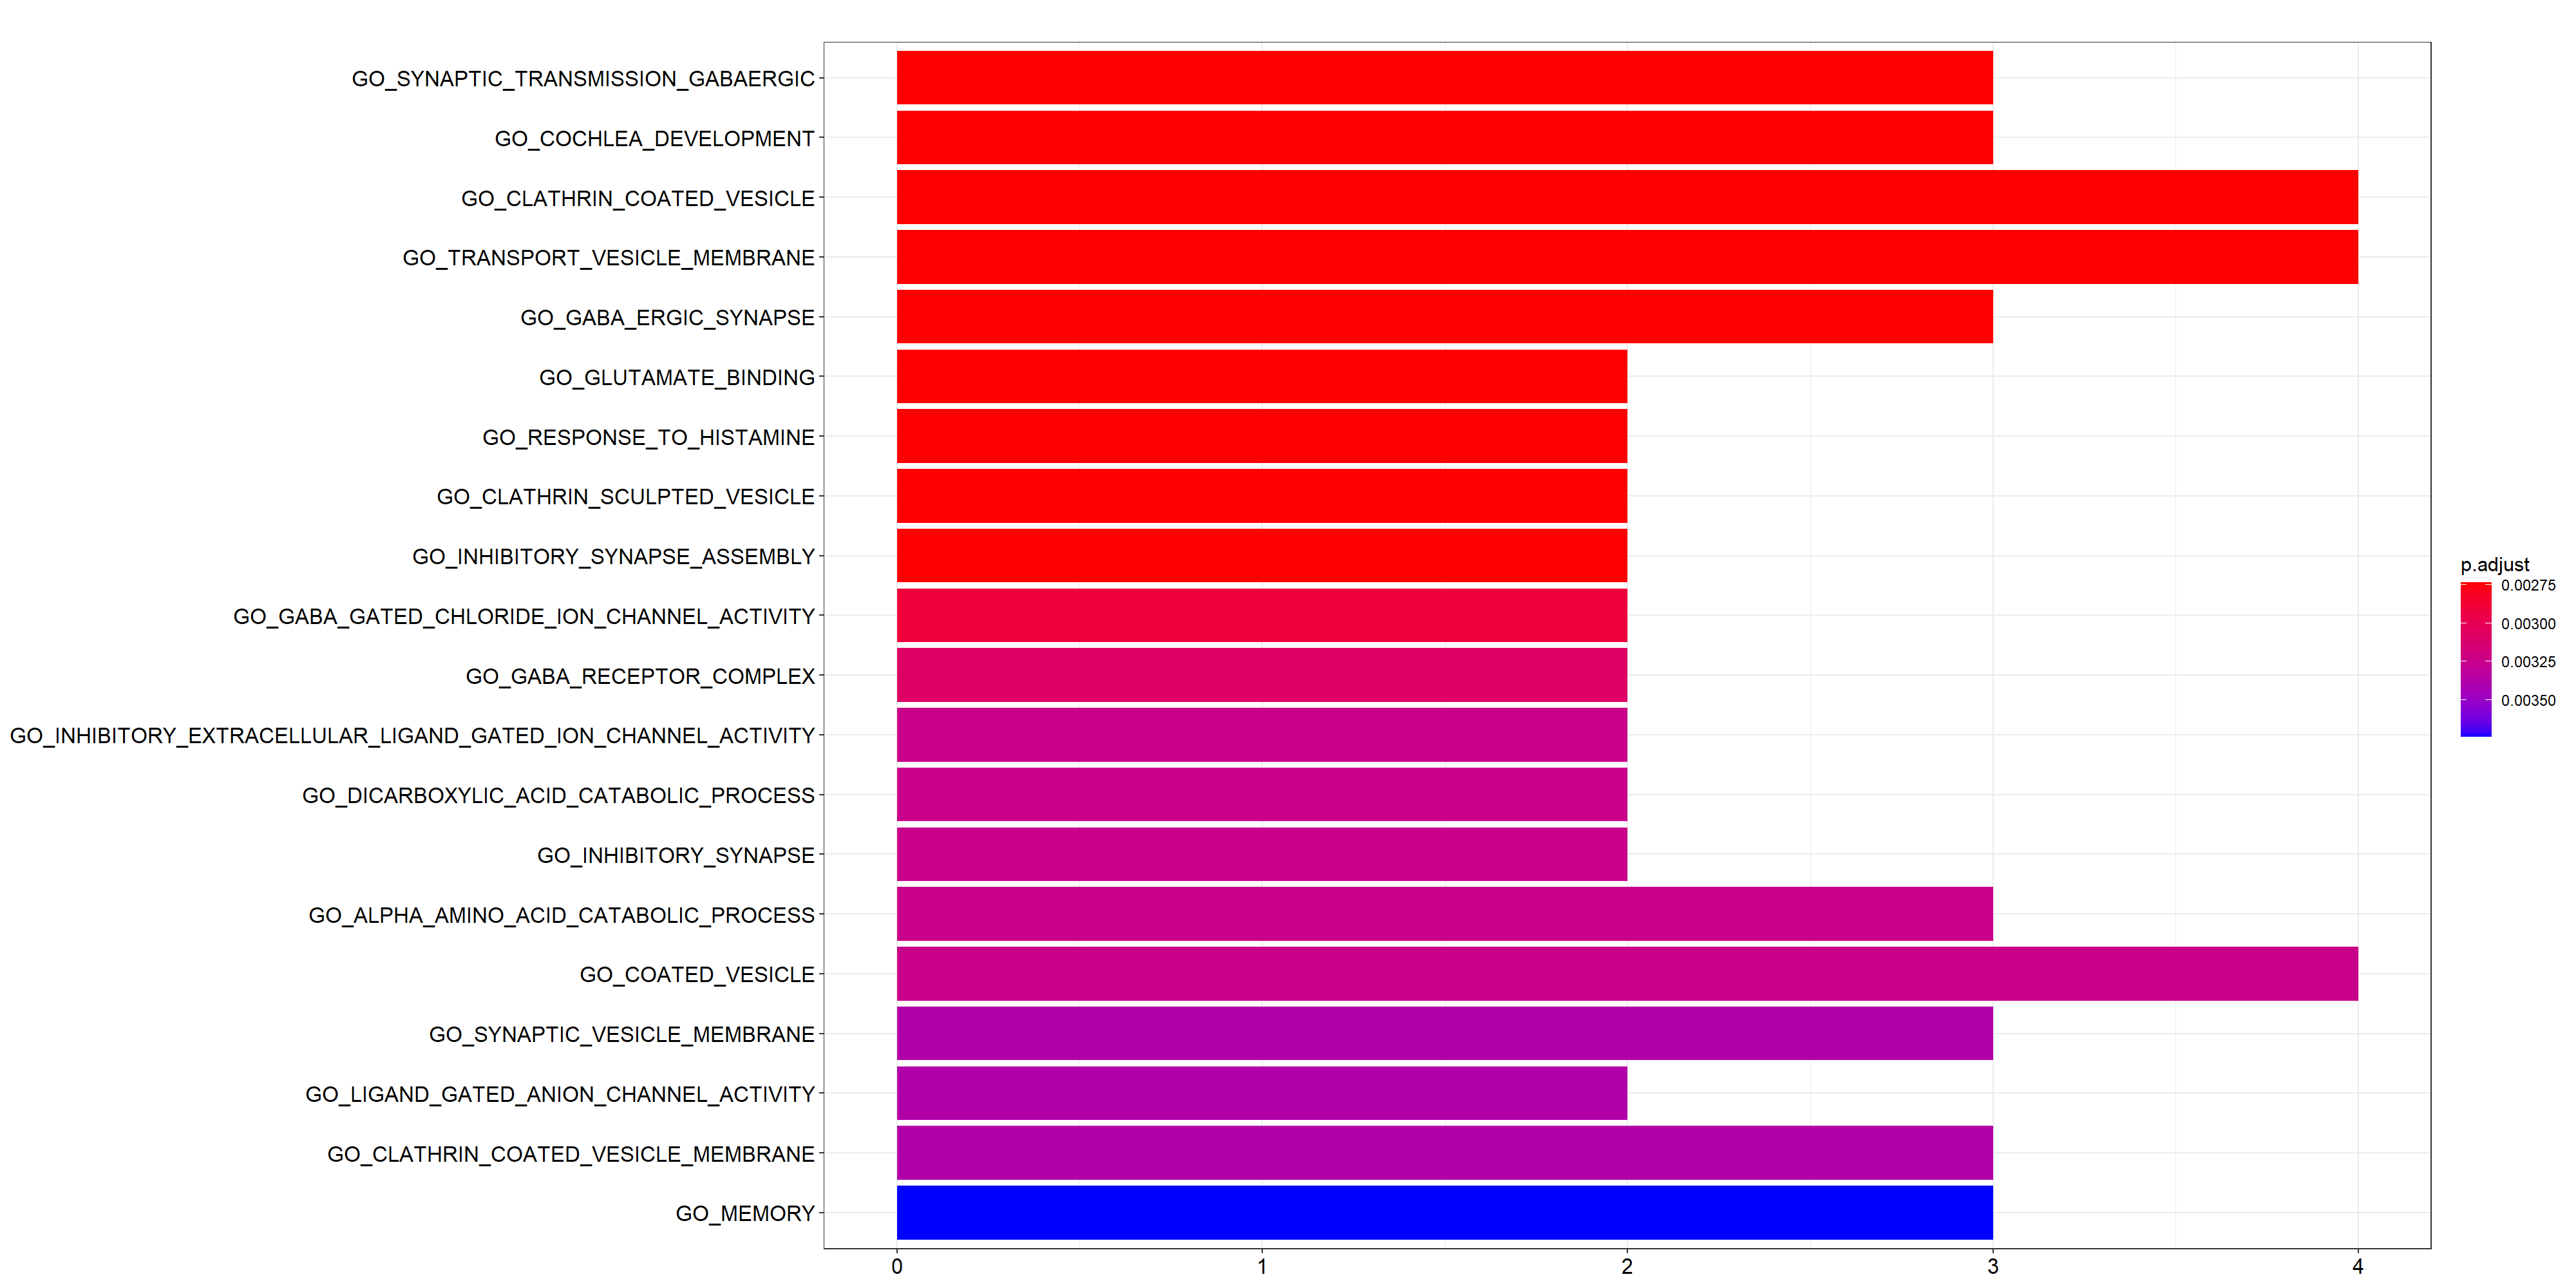
\includegraphics[width=5cm]{Figures/Path/CTLvsAD_ef_barplot-hip.png} }}%
    \qquad
    \subfloat{{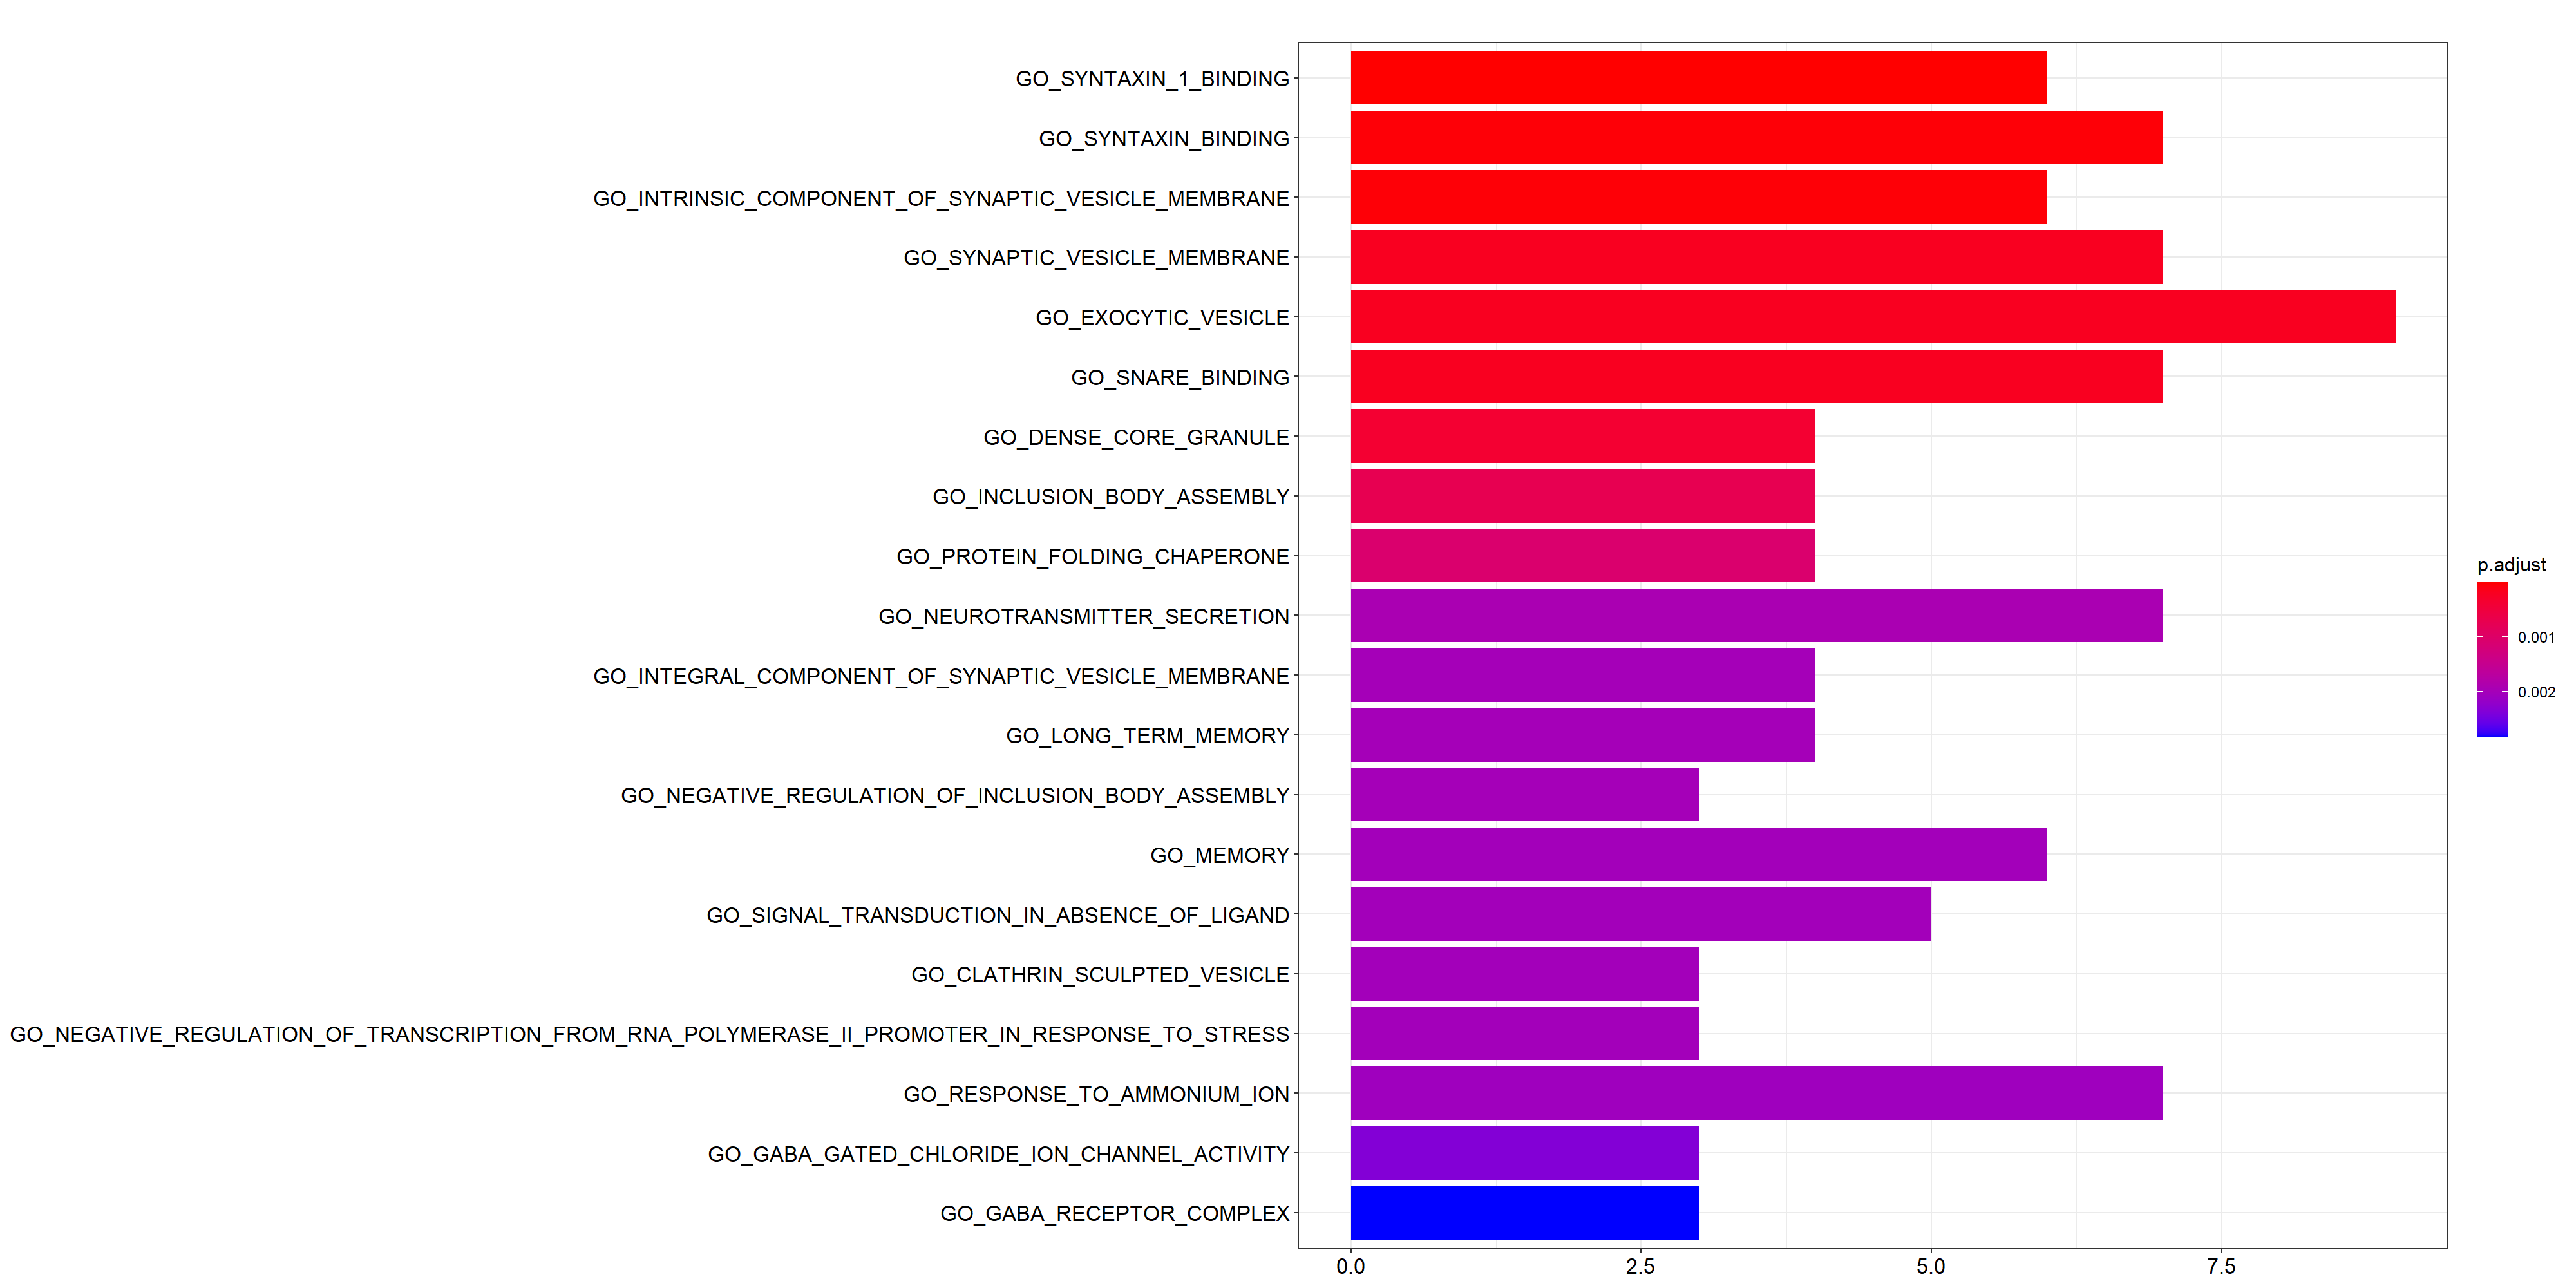
\includegraphics[width=5cm]{Figures/Path/CTLvsAD_em_barplot-hip.png} }}%
    \\
    \subfloat{{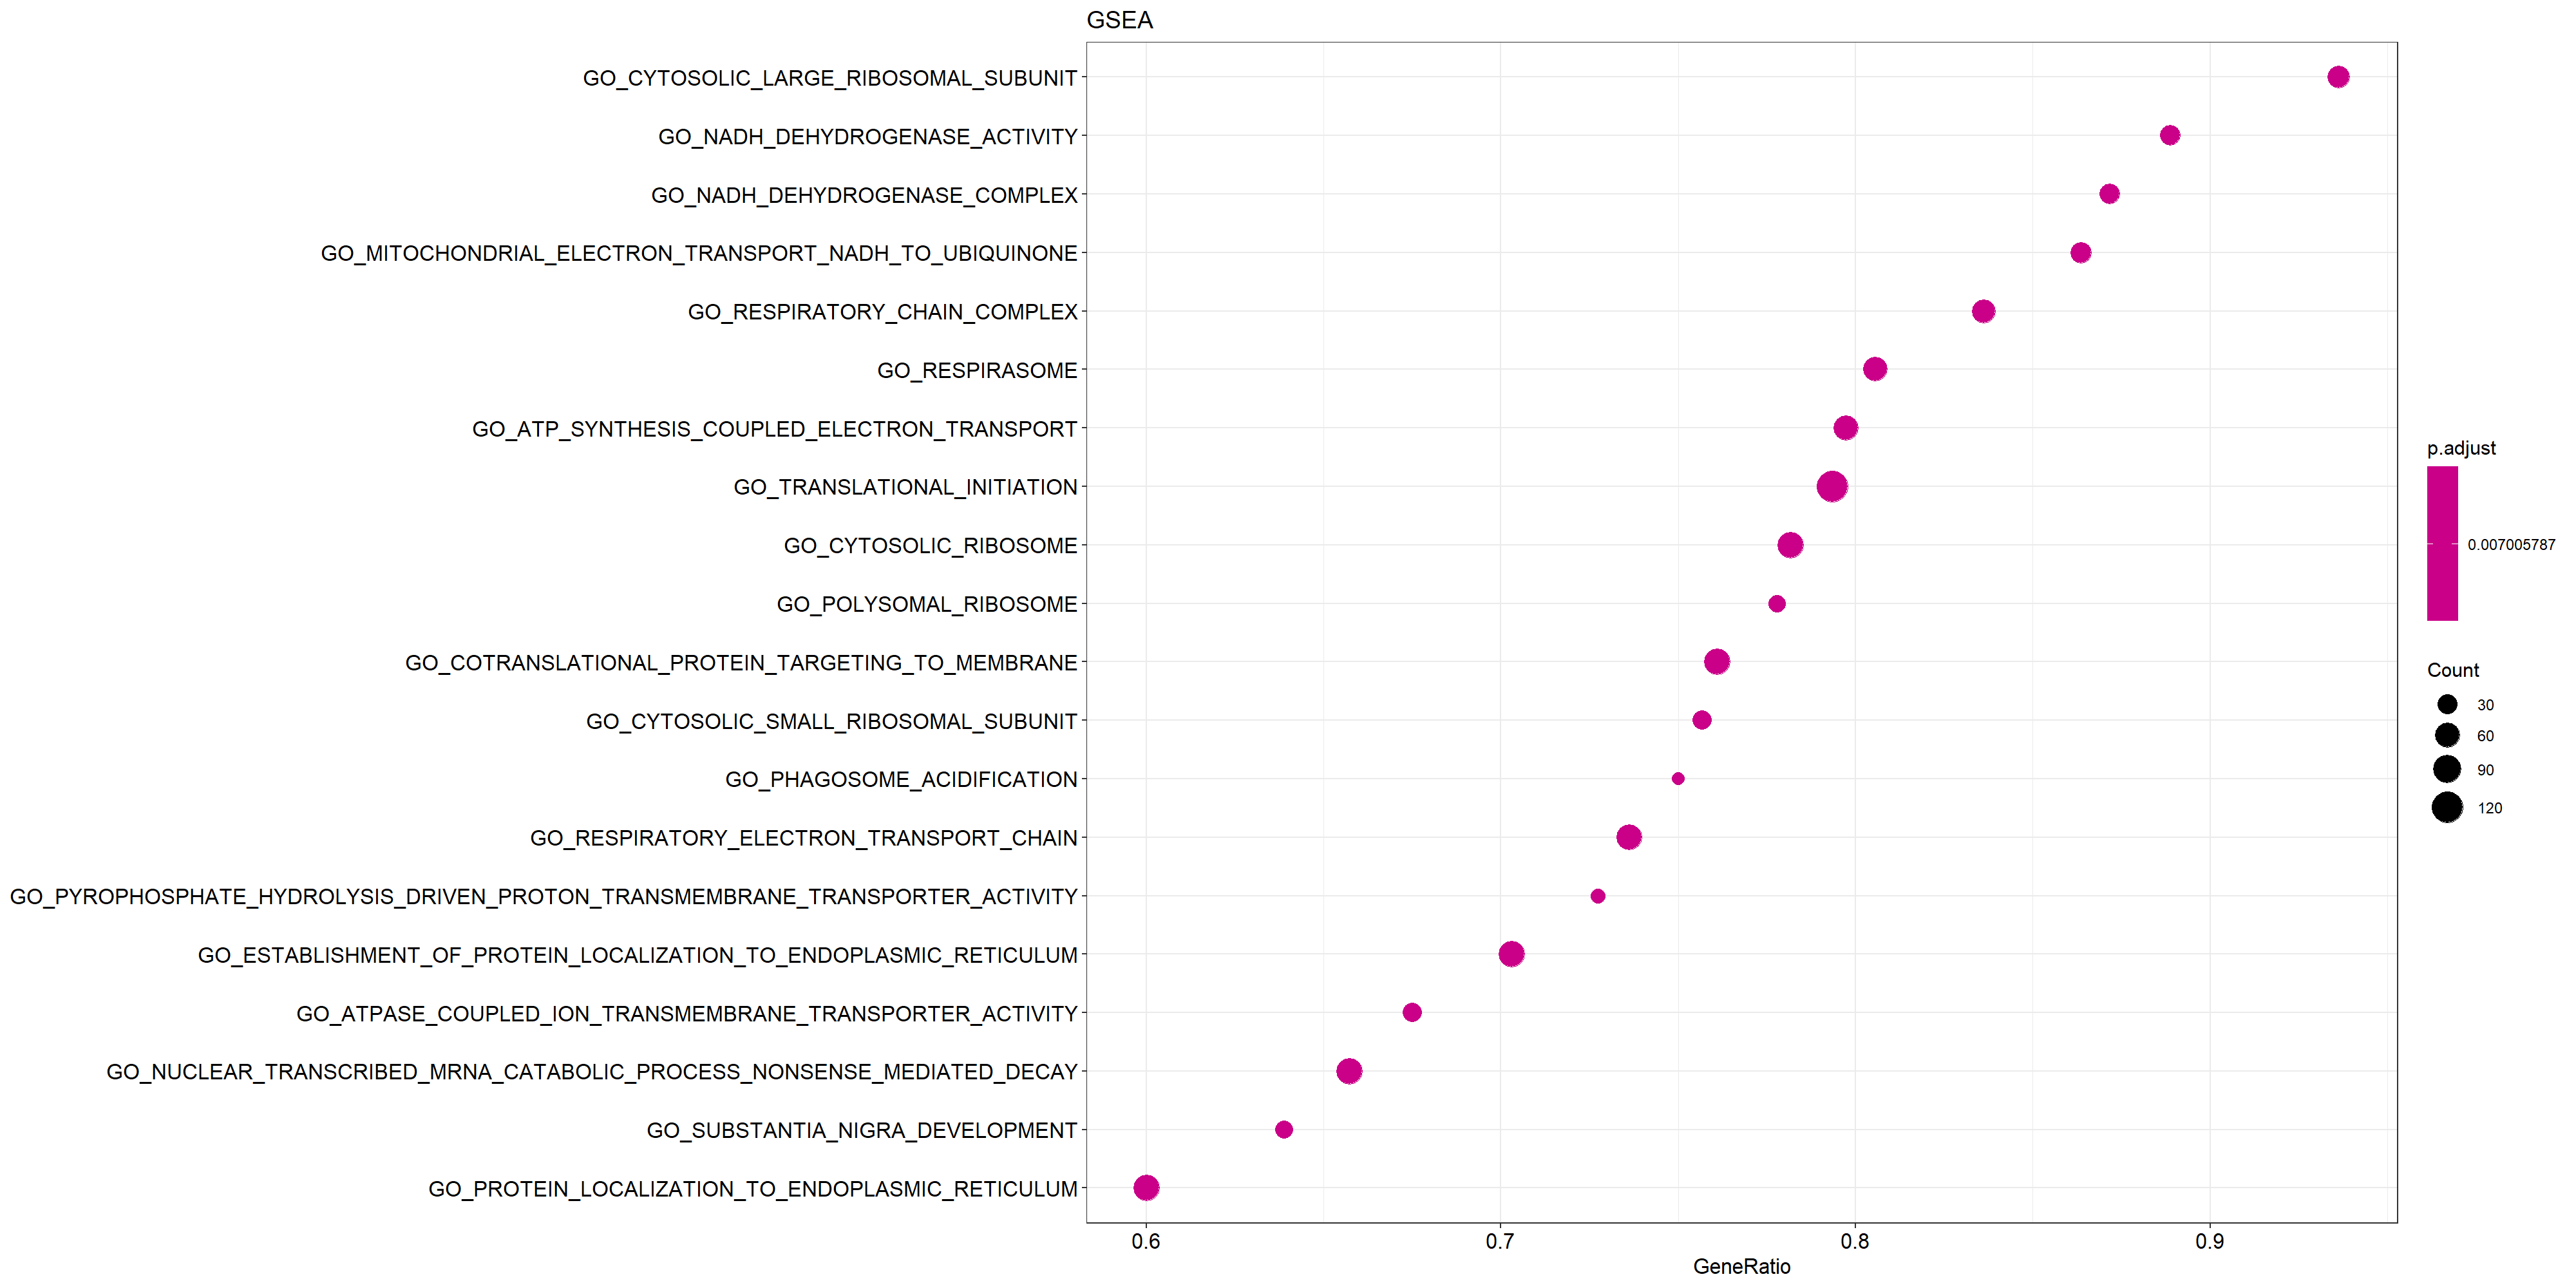
\includegraphics[width=5cm]{Figures/Path/CTLvsAD_ef_dotplot-hip.png} }}%
    \qquad
    \subfloat{{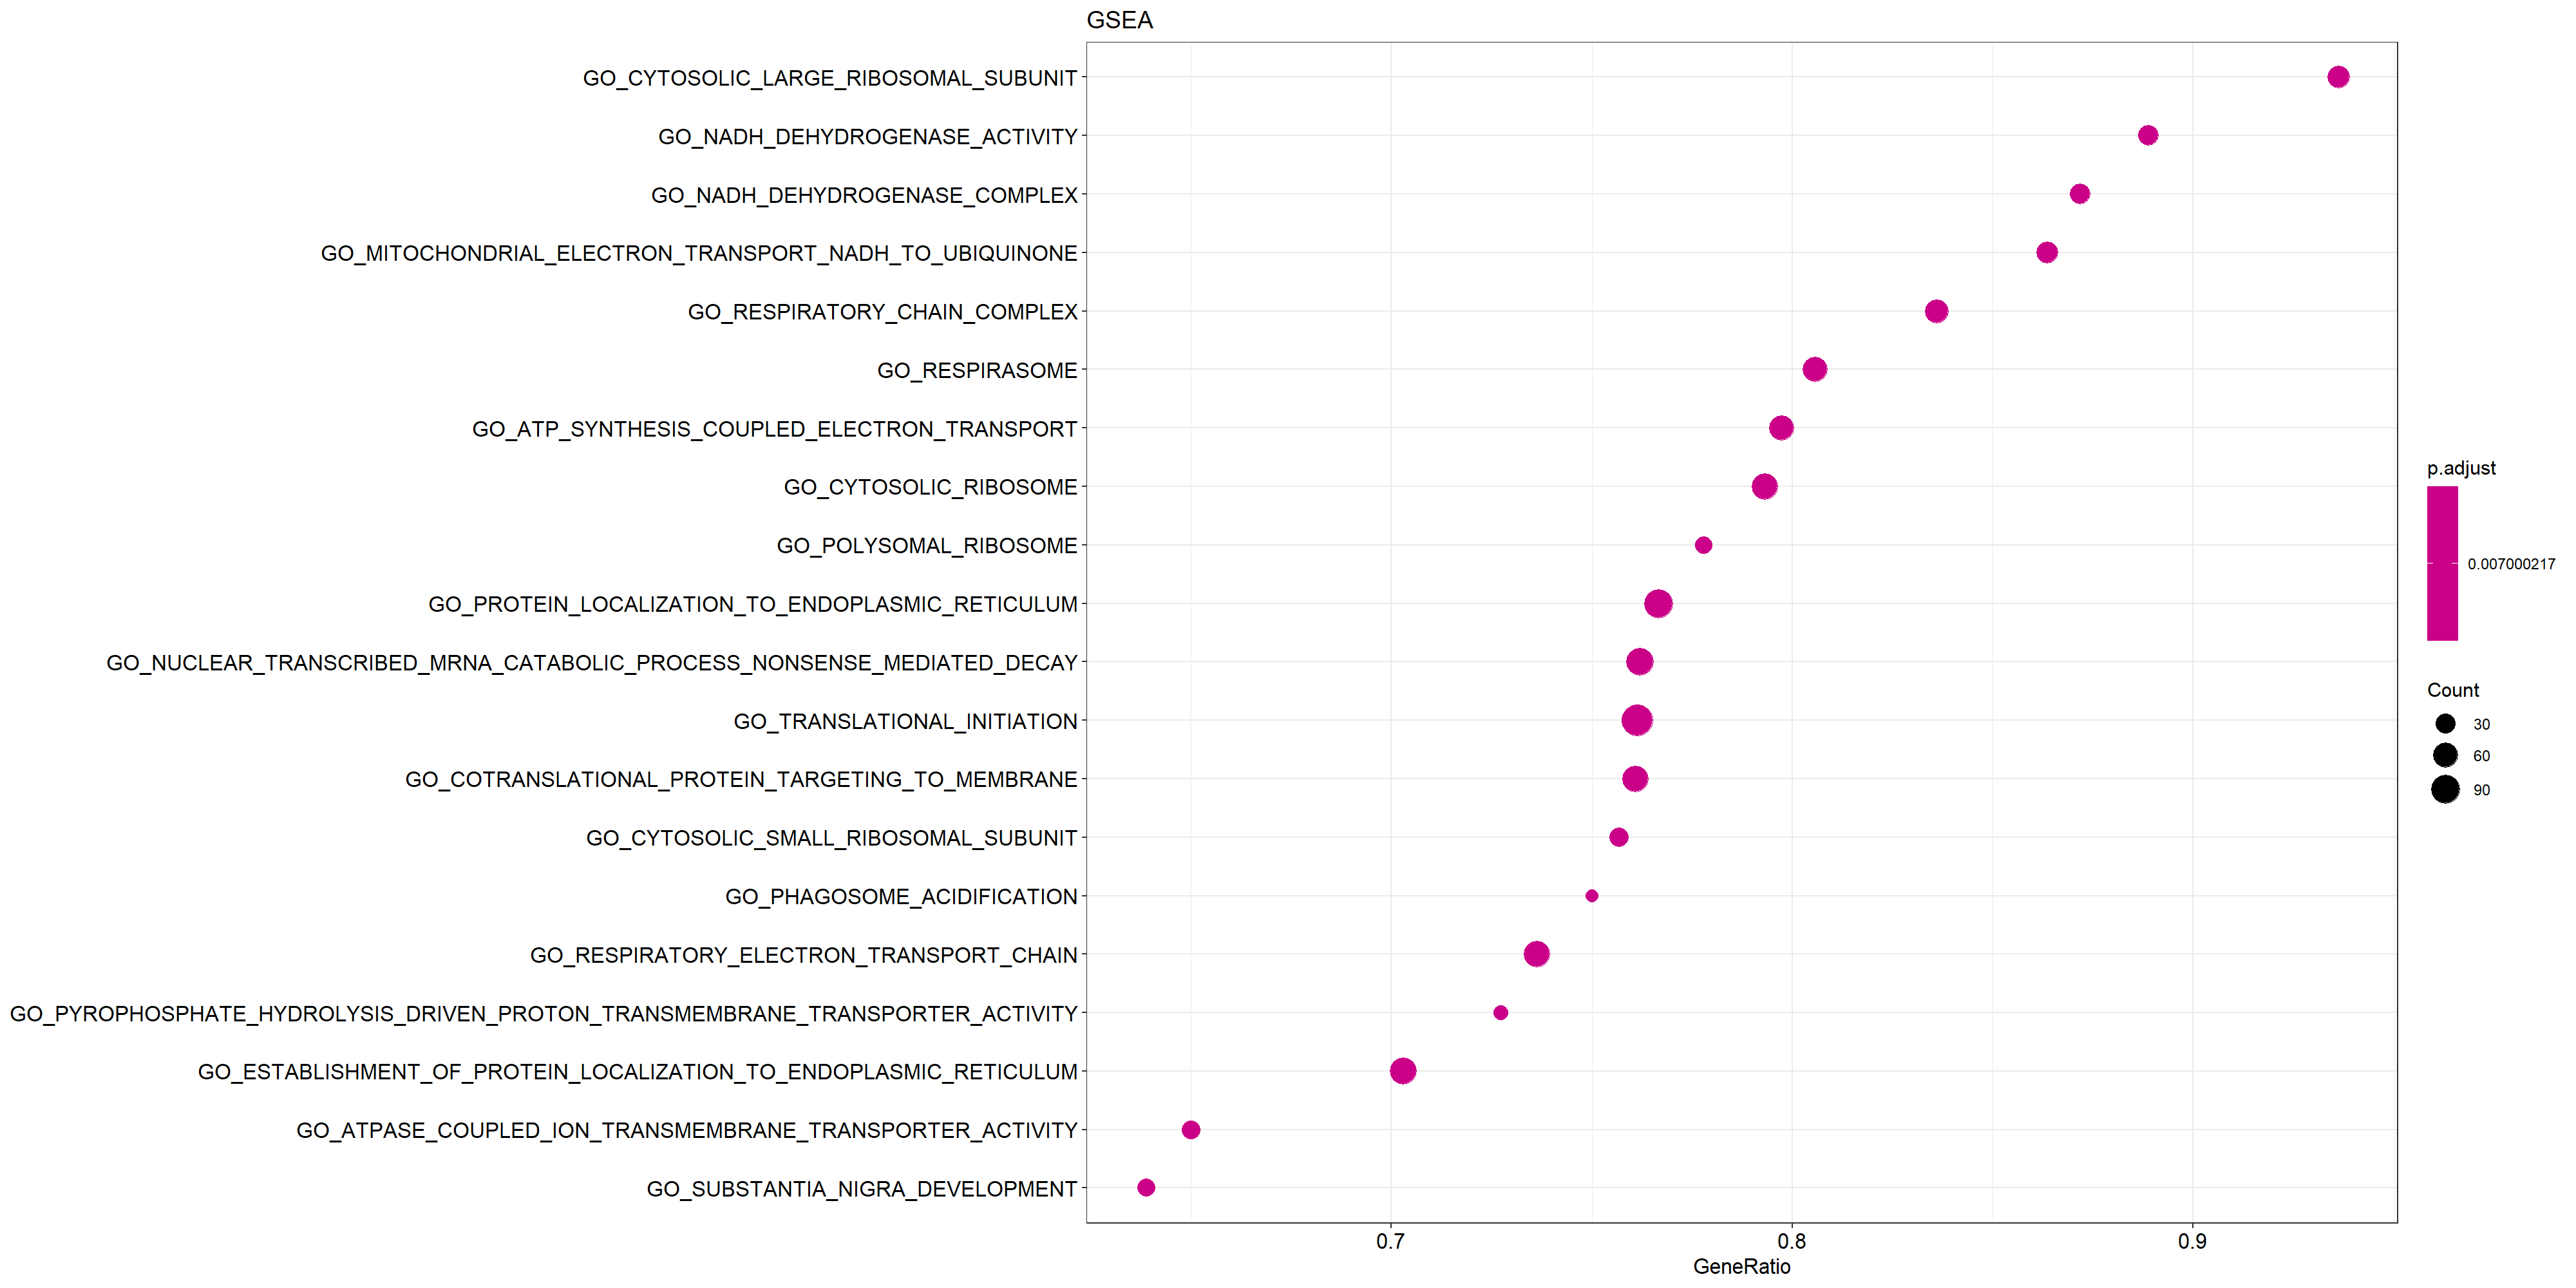
\includegraphics[width=5cm]{Figures/Path/CTLvsAD_em_dotplot-hip.png} }}%
\caption{Bar plot and dot plot visualization for over representation analysis and gene set enrichment analysis, respectively, of Hip-AD.}
\footnotesize Left for female; right for male.
\label{fig:path-hip-ad}%
\end{figure}

When the DEGs obtained from the comparison among female and male sets were introduced to ORA, the following paths were resulted (Appendix \ref{paths-comparison}). Since the unique up-regulated genes of the female set were only three, the ORA could not give any result. Hence, a brief description of the genes is given. NCALD is a neuronal calcium sensor which is related to neurotransmitter receptor binding and downstream transmission in the postsynaptic cell pathways. ROCK1P1 is a pseudogene of rho associated coiled-coil containing protein kinase 1. RNVU1, an snRNA, is involved in RNA transport and mRNA splicing major pathway. What is more, the male related pathways are synapse, sintaxin binding and secretion, and neuron projection. The common routes are synapse, neuron projection, cell-cell signaling, and nervous system processes. For the down-regulated genes, the common genes are: CDR1 (cerebellar degeneration protein 1), AEBP1 (adipocyte enhancer binding protein 1), RNU11 (RNA, U11 small nuclear), LOC284412 (lncRNA), and MTSS1L (metastasis suppressor 1-like). The exclusive male pathways are related to inclusion bodies, incorrect protein folding, and signal transduction in absence of ligand. The unique female genes are PCDHGA12 and MT1F. The former is a neural cadherin-like protein and plays a critical role in the establishment and function of specific cell-cell connections in the brain. The latter is a SLC transporter and is involved in copper homeostasis.

\textbf{Front-AD.} In this dataset, the female and male ORA results are resembling (32/40 similarities), as seen in Fig. \ref{fig:path-front-ad}. The difference is that the female set contains more paths related to postsynapse and the male comprises more routes associated to cation channels. Nevertheless, the GSEA pathways are completely different. The male part is related to protein localization, cytosolic ribosome, mRNA splicing, oxidative stress neuron death, and myelin sheath. The female section includes protein localization, synapses, axon, clathrin endocytosis, cell communication by electric coupling, and cell cortex region pathways. Moreover, when the unique DEGs are introduced to the analysis, the same routes are output among the sexes but with opposite direction, as mentioned in previous ideas; also, the intersection is empty.

\begin{figure}[!ht]%
    \centering
    \subfloat{{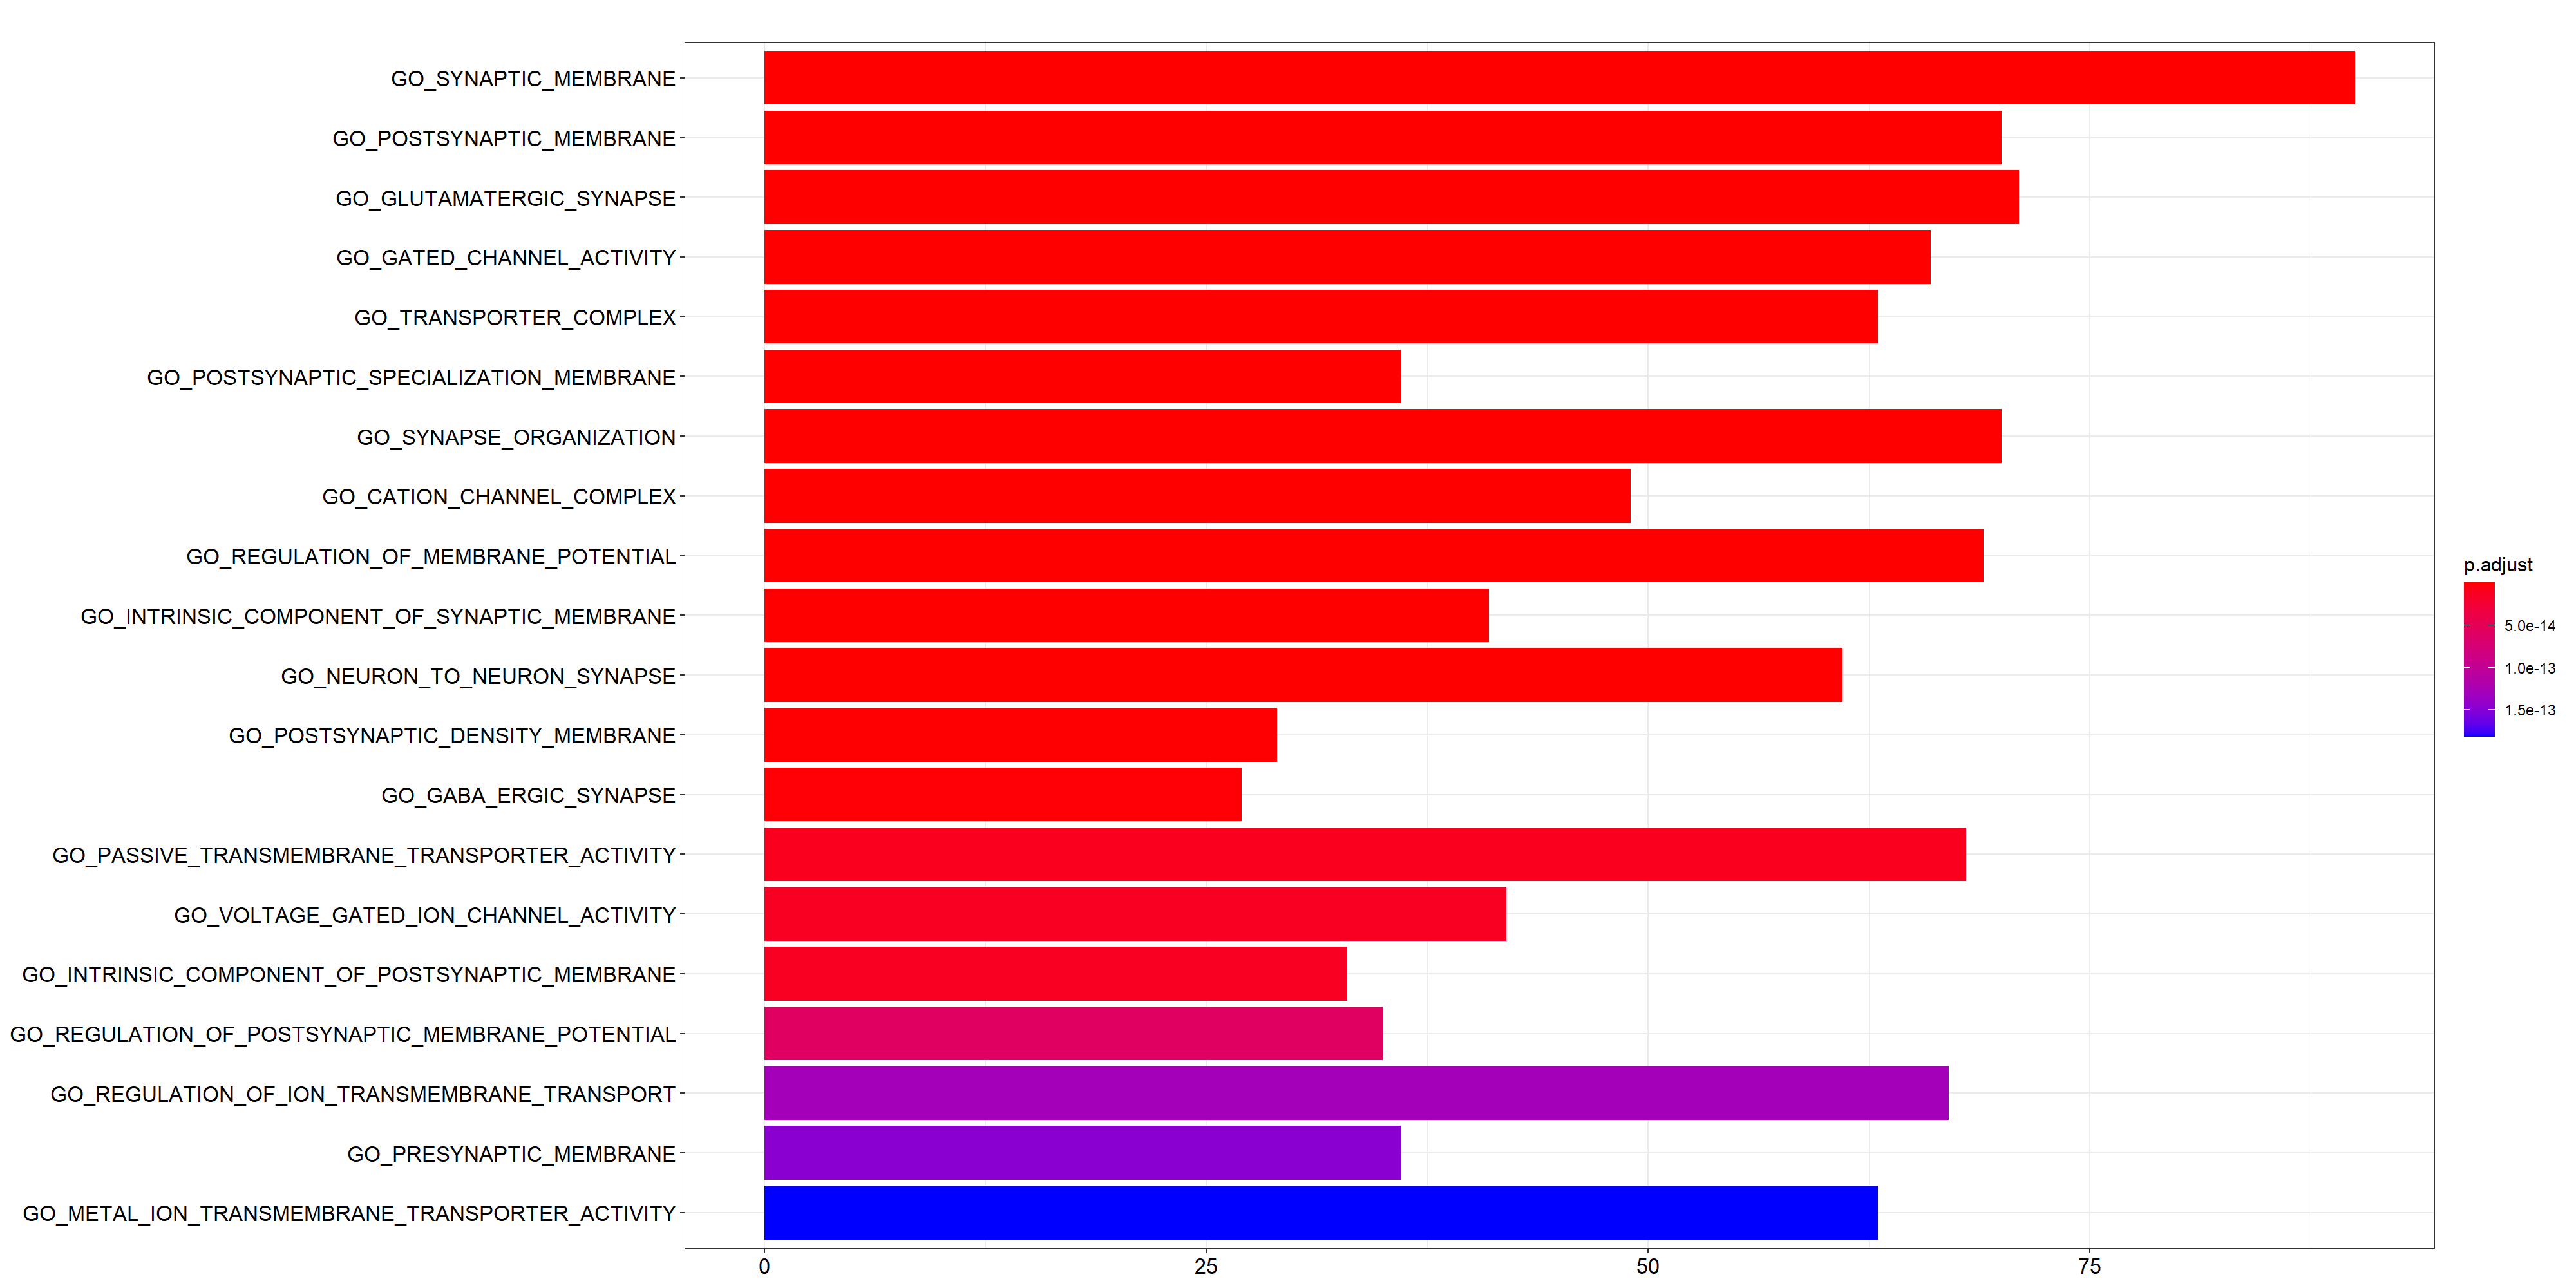
\includegraphics[width=5cm]{Figures/Path/CTLvsAD_ef_barplot-front.png} }}%
    \qquad
    \subfloat{{\includegraphics[width=5cm]{Figures/Path/CTLvsAD_em_barplot-front.png} }}%
    \\
    \subfloat{{\includegraphics[width=5cm]{Figures/Path/CTLvsAD_ef_dotplot-front.png} }}%
    \qquad
    \subfloat{{\includegraphics[width=5cm]{Figures/Path/CTLvsAD_em_dotplot-front.png} }}%
\caption{Bar plot and dot plot visualization for over representation analysis and gene set enrichment analysis, respectively, of Front-AD.}
\footnotesize Left for female; right for male.
\label{fig:path-front-ad}%
\end{figure}

\textbf{Fus-AD.} In Fig. \ref{fig:path-fus-ad}, the ORA results are presents for both sexes. The female set has been associated with synapse processes, transport of ions, and neurotransmitters processes. The male set contains synapse processes, neurotransmitter transport and secretion, and transport by channels, as well. As it can be observed, female and male results are similar in ORA as well as in GSEA. The female genes are related to respiration and synapse; interesting brain paths are tau protein binding, substantia nigra development, neural nucleus development, and main axon. For the counterpart set, it has enriched pathways linked to mainly respiration, synapse and the same interesting brain paths.

When the intercepted genes among both sexes of Section \ref{res-dgea} are fed to ORA the specific enriched pathways are obtained (Appendix \ref{paths-comparison}). For the up-regulated genes, both sexes have routes related to synapse processes, neuron projection, and cell-cell signaling. Additionally, motile cilium pathway was the only enriched exclusively for male. The female DEGs were associated with synapse processes, neuron projection, cell-cell signaling, neuron differentiation, and ion transport. For the down-regulated genes, the intersection contained biological adhesion, morphogenesis, and defense response. The male genes were linked with response to zinc and copper, and detoxification of inorganic compounds; while the female DEGs related to immune system and inflammation, and cell activation.

\begin{figure}[!ht]%
    \centering
    \subfloat{{\includegraphics[width=5cm]{Figures/Path/CTLvsAD_ef_barplot-fus.png} }}%
    \qquad
    \subfloat{{\includegraphics[width=5cm]{Figures/Path/CTLvsAD_em_barplot-fus.png} }}%
    \\
    \subfloat{{\includegraphics[width=5cm]{Figures/Path/CTLvsAD_ef_dotplot-fus.png} }}%
    \qquad
    \subfloat{{\includegraphics[width=5cm]{Figures/Path/CTLvsAD_em_dotplot-fus.png} }}%
\caption{Bar plot and dot plot visualization for over representation analysis and gene set enrichment analysis, respectively, of Fus-AD.}
\footnotesize Left for female; right for male.
\label{fig:path-fus-ad}%
\end{figure}

The molecular subtypes of Fus-AD-f obtained similar over represented pathways; the three subtypes are related to synapse processes and transportation of ions through channels. S2 is also represented by secretion, and S3 with neurotransmitter transport and secretion. Additionally, the dot plots in Fig. \ref{fig:path-fus-f-sub} show that the three subtypes are associated with immune system and inflammation, and vascular development; S3 also has pathways of extracellular matrix. For the male counterpart, the results can be appreciated in Fig. \ref{fig:path-fus-m-sub}. The ORA relates the DEGs of S1 with ion transport, and synapse processes, while S2 is associated with synapse, neuron projection, neurotransmitter transport, cognition, memory and locomotory behaviour. For GSEA, both subtypes were enriched in immune system and inflammation, and vascular development.

\begin{figure}[!ht]%
    \centering
    \subfloat[\centering ORA for S1. ]{{\includegraphics[width=5cm]{Figures/Path/CTLvs1_ef_barplot-fus.png} }}%
    \qquad
    \subfloat[\centering GSEA for S1. ]{{\includegraphics[width=5cm]{Figures/Path/CTLvs1_ef_dotplot-fus.png} }}%
    \\
    \subfloat[\centering ORA for S2. ]{{\includegraphics[width=5cm]{Figures/Path/CTLvs2_ef_barplot-fus.png} }}%
    \qquad
    \subfloat[\centering GSEA for S2. ]{{\includegraphics[width=5cm]{Figures/Path/CTLvs2_ef_dotplot-fus.png} }}%
    \\
    \subfloat[\centering ORA for S3. ]{{\includegraphics[width=5cm]{Figures/Path/CTLvs3_ef_barplot-fus.png} }}%
    \qquad
    \subfloat[\centering GSEA for S3. ]{{\includegraphics[width=5cm]{Figures/Path/CTLvs3_ef_dotplot-fus.png} }}%
\caption{Bar plot and dot plot visualization for over representation analysis and gene set enrichment analysis, respectively, of sutbype in Fus-AD-f.}
\label{fig:path-fus-f-sub}%
\end{figure}

\begin{figure}[!ht]%
    \centering
    \subfloat[\centering ORA for S1. ]{{\includegraphics[width=5cm]{Figures/Path/CTLvs1_em_barplot-fus.png} }}%
    \qquad
    \subfloat[\centering GSEA for S1. ]{{\includegraphics[width=5cm]{Figures/Path/CTLvs1_em_dotplot-fus.png} }}%
    \\
    \subfloat[\centering ORA for S2. ]{{\includegraphics[width=5cm]{Figures/Path/CTLvs2_em_barplot-fus.png} }}%
    \qquad
    \subfloat[\centering GSEA for S2. ]{{\includegraphics[width=5cm]{Figures/Path/CTLvs2_em_dotplot-fus.png} }}%
\caption{Bar plot and dot plot visualization for over representation analysis and gene set enrichment analysis, respectively, of sutbype in Fus-AD-m.}
\label{fig:path-fus-m-sub}%
\end{figure}

Finally, the distribution of the DEGs in the Venn diagrams of Section \ref{res-dgea} are used to examine the common and exclusive pathways of each tissue and/or condition; these results can be found in Appendix \ref{paths-comparison}. 

First, the blood and prefrontal cortex tissues with HD are compared. For the up-regulated genes, no intersection was found. Hence, the enriched pathways for Blood-HD-f are related to cytosolic ribosome; for Blood-HD-m are linked to abnormality of abdominal organs, cellular macromolecule localization, and chromosome organization. PCx-HD was enriched with intrinsic component of plasma membrane, synapse, neuron projection, and neurotransmitter receptor activity. For the down-regulated genes, few genes were placed in the intercept between HD-Blood-m and PCx-HD, then the description of each gene is provided. CXCL1 plays a role in inflammation and is associated with certain tumors. CPVL is related to proteolysis. IL18R1 encodes a cytokine receptor that binds to interleukin 1 family. STX11 is a syntaxin which has been implicated in fusion of intracellular transport vesicles. ANG is a potent mediator of new blood vessel formation. ESM1 is involved in lung endothelial cell-leukocyte interactions. The exclusive pathways enriched for PCx-HD are related to defense response, cell activation, and inflammatory response. Additionally, the unique pathway of Blood-HD-f is specific granule lumen; and Blood-HD-m has been related to abnormality of connective tissue, and endoplasmic reticulum. 

Second, similar tissues with different conditions are compared. The under-expressed intersection between PCx-HD and PCx-PD resulted in pathways related to immune system response and inflammation, while the common routes among Front-AD-f and PCx-HD are about epithelium development, cell differentiation, biological adhesion, and inflammatory response. Front-AD-f and PCx-PD have in common cell activation, immune system processes, and secretion pathways. The three tissues already mentioned share immune system and inflammation, and apoptotic process routes. The unique pathways of PCx-HD are related to extracellular matrix, defense response, and tube morphogenesis. PCx-PD was associated with transport, secretion and response to abiotic stimulus. The female set of the frontal tissue obtained cell motility, biological adhesion, vascular development, and immune system response. The male counterpart resulted with synapse, neuron projection, cell-cell signaling, axon, neuron development, and dendritic tree.

For the over-expressed genes, the pathways linked to PCx-HD and PCx-PD are receptor signaling, plasma membrane, synapse, and hormone mediated apoptotic signaling. Front-AD-f and PCx-HD have in common synaptic pathways, as well as Front-AD-f and PCx-PD, and the intercept of the three datasets. PCx-PD was associated with neuropeptide signaling, G protein receptor signaling, and nervous system processes pathways. In addition, Front-AD-f was linked to synapse, neuron projection, and neurogenesis, while the male counterpart was related to biological adhesion, cell activation, apoptotic process, and immune system processes.

The third comparison was made between the different tissues with AD for male. In order to be concise, the must repeated pathways among the comparisons will be expressed here. The up-regulated DEGs employed in these comparisons were predominantly associated with synapse, neuron projection, cell adhesion, axon, and transport. An interesting event is that AD-Front-m was the only enriched in apoptotic process and immune system. Moreover, all the tissues except frontal were related with behavior. Also, fusiform gyrus and hippocampus were associated with GABA receptor and channels. For the under-expressed genes, many comparisons did not obtain any overlap with gene sets or have too few DEGs to reach a result. Fus-AD-m and Hip-AD-m shared pathways related to inclusion body, unfolded protein binding, and protein folding. Temporal and parietal share synapse structural plasticity route, while parietal has as unique path cell differentiation. Fusifurm gyrus was linked to cell activation, vascular development and inflammatory response. Lastly, frontal obtained brain related pathways which were enriched by the others in the over-expressed side.

Finally, the fourth comparison was carried out with the female AD tissues. As before, the interpretation is brief for the over-expressed genes. The majority of the comparisons were related to synaptic processes, cell adhesion, nervous system processes, neuron projection, and transport. Several intersection had few DEGs to get results from the analysis, and others did not overlapped. For the under-expressed genes, varying pathways were enriched. The repeated routes were about vascular development, cell and neuron differentiation, and immune system and inflammatory response. On the other hand, frontal, temporal and parietal tissues obtained oligodendrocyte development, and astrocyte projection pathways. Pa-AD-f was associated with mitochondrial respiratory chain defects, and optic atrophy.


\section{Drug repurposing}

The penultimate assessment done with the results of DEG analysis was drug repurposing. As detailed in Section \ref{drug-method}, this examination uses the direction of each gene LFC in order to compare them with the drug perturbation signature database. In the following lines, three repurposed drugs are given alongside a brief explanation of how that specific drug could attack the condition. Moreover, the resulting drugs are presented in Table \ref{tab:drugs}.

\begin{table}[!ht]
\small
\centering
\caption{Repurposed drugs according to the disease, tissue and sex of the samples.}
\label{tab:drugs}
\begin{tabular}{l|ll}
\hline
\multicolumn{1}{c|}{\textbf{Disease}} & \multicolumn{1}{c}{\textbf{Tissue}} & \multicolumn{1}{c}{\textbf{Drug}} \\ \hline
\textbf{PD} & Prefrontal cortex & Flurbiprofen                 \\
            &                   & Simvastatin                  \\
            &                   & Mometasone furoate           \\ \hline
\textbf{HD} & Prefrontal cortex & Lovastatin                   \\
            &                   & Statin                       \\
            &                   & Amitriptyline                \\
            &                   & Pridopidine                  \\
            & Blood-f           & Sulfachlorpyridazine         \\
            &                   & Benzamil                     \\
            &                   & Flumethasone                 \\
            & Blood-m           & Remoxipride                  \\
            &                   & Zardaverine                  \\
            &                   & Ginkgolide A                 \\ \hline
\textbf{AD} & Parietal-f        & Ascorbic acid                \\
            &                   & Meptazinol                   \\
            &                   & NS-398                       \\
            & Parietal-m        & Cinnarizine                  \\
            &                   & Vinpocetine                  \\
            &                   & Bumetanide                   \\
            & Temporal-f        & Acetyl salicylsalicylic acid \\
            &                   & Lovastatin                   \\
            &                   & Astemizole                   \\
            & Temporal-m        & Molindone                    \\
            &                   & Acetyl salicylsalicylic acid \\
            &                   & Ketorolac                    \\
            & Hippocampus-f     & Cyanocobalamin               \\
            &                   & Omeprazole                   \\
            &                   & Gemfibrozil                  \\
            & Hippocampus-m     & Acetyl salicylsalicylic acid \\
            &                   & Bucladesine                  \\
            &                   & Metrizamide                  \\
            & Frontal-f         & NS-398                       \\
            &                   & Trichostatin A               \\
            &                   & Decitabine                   \\
            & Frontal-m         & Clenbuterol                  \\
            &                   & Etiocholanolone              \\
            &                   & Mephentermine                \\
            & Fusiform-f        & Astemizole                   \\
            &                   & Prestwick-1080               \\
            &                   & Acetyl salicylsalicylic acid \\
            & Fusiform-m        & Molindone                    \\
            &                   & Nystatin                     \\
            &                   & Prestwick-1080               \\ \hline
\end{tabular}
\end{table}

\textbf{PCx-PD.} Flurbiprofen is one of the most potent non-selective anti-inflammatory agents; studies in mice have shown noteworthy neuroprotective activity against motor impairment and microglia activation \cite{lepiscopo}. Simvastatin is a cholesterol-lowering drug which have proofed to have neuroprotective properties; a drug trial aimed at determining whether this drug has the potential to slow down the progression of PD \cite{carroll}. It finished on September, 2020, however, the results have not been published. Lastly, mometasone furoate has been mentioned in the context of PD accompanied by Miglustat medicine according to information in MalaCards \cite{mometasona}.

\textbf{PCx-HD.} Lovastatin has shown to protect the neural stem cells against cell death induced by oxidative stress, which has been implicated in several NDs \cite{abdanipour}. Statin was used in patients with premotor HD and was associated with delayed motor diagnosis of HD \cite{schultz}. In mice HD model, amitriptyline has demonstrated to improve motor function by enhancing neurotrophin signaling and mitochondrial functions \cite{cong}.

\textbf{Blood-HD-f.} Sulfachlorpyridazine activates the adaptive response to hypoxia, which is a novel therapeutic strategy for NDs. This medicine can penetrate into the central nervous system and may be employed to treat diseases associated with oxidative neuronal death \cite{aleyasin}. Mouse models treated with benzamil have shown a markedly reduction of the huntingtin- polyglutamine aggregation; this drug was able to ease the inhibition of the ubiquitin-proteasome activity and enhancing the degradation of these aggregations in pathological range \cite{wong}. Lastly, flumethasone has been used to increase the potential of haloperidol (to treat HD chorea) according to DrugBank database \cite{wishart}.

\textbf{Blood-HD-m.} Remoxipride, a neuroleptic agent, is a selective medicine that binds to dopaminergic receptor D2; a chronic treatment with this drug in monkeys regulated this receptor. This drug may be used in HD since this condition has hyperdopamine signs \cite{lidow}. Additionally, the results of the study \cite{hu} also contains remoxipride as a treatment for HD effects. A current description of the potential reduction of PDE4D allosteric modulators may be an approach for alleviating HD; zardaverine is a PDE4 inhibitor \cite{azevedo}. Ginkgolide A is a leaf extract with protective effects against NDs due to its antioxidant properties and anti-platelet activating factor activity; \textit{in vivo} and \textit{in vitro} studies have supported its neuroprotective effects \cite{choudhary}.

\textbf{Pa-AD-f.} Concentrations of plasma vitamin C was identified as low in patients with AD and dementia \cite{dasilva}; hence, an external dose of ascorbic acid may ameliorate the symptoms. The experiments in \cite{shi} concluded that meptazinol appears to be an effective AChE inhibitor for the treatment of AD, and it has properties for relieving symptoms and modifying the pathogenesis in mice. NS-398, a cyclooxygenase-2 inhibitor, partially prevented the suppression of long-term plasticity by the amyloid-$\beta$ protein \cite{kotilinek}.

\textbf{Pa-AD-m.} Cinnarizine is an anti-vertigo agent, but it can also be seen as a nootropic drug due to its vasorelaxating properties (increases elasticity of the cell wall) boosting oxygen to the brain \cite{deka}. Vinpocetine, a synthetic derivative of an extracted molecule of a seed, has been indicated for treatment of cerebrovascular disorders in Asia and Europe \cite{zhang2018}. Bumetanide is used to treat high blood pressure, and distinct classes of anti-hypertensive drugs has been associated with a reduction of AD risk \cite{chuang}.

\textbf{Temp-AD-f.} Acetyl salicylsalicylic acid, the common Aspirin, has demonstrated to have a beneficial effect on AD as a therapeutic agent \cite{choi}. The explanation for lovastatin was given above, refer to PCx-HD in this section. Astemizole, an allergy remedy, was tested in \cite{rojo} with anomalous AD aggregates of tau protein; it was found that the drug specifically binds to these aggregates.

\textbf{Temp-AD-m.} Molindone is a anti-psychotic agent which has been employed to control delusions, hallucinations and psychomotor agitation of AD patients with behavior or mood disorders \cite{cummings}. Acetyl salicylsalicylic acid has been described for the female dataset above. Cyclooxygenase enzyme activity is involved in AD neuroinflammation; non-steroidal anti-inflammatory agents, such as ketorolac, act as inhibitors of this enzyme as well of amyloid-$\beta$ aggregation \cite{ali}. 

\textbf{Hip-AD-f.} AD patients have been associated with low plasma levels of cyanocobalamin, also known as vitamin B12; more research is needed in order to elucidate if the neuroinflammatory effect of cobalamin is involved in AD pathophysiology \cite{politis}. Omeprazole has \textit{in vitro} evidence indicating that it might have neuroprotective and anti-inflammatory effects \cite{ortiz}. Gemfibrozil, a drug for hyperlipidemia, has demonstrated to lower the amyloid plaque abundance, reduce microgliosis and astrogliosis in AD animal models \cite{chandra}.

\textbf{Hip-AD-m.} Acetyl salicylsalicylic acid has been previously described in the description for Temp-AD-f. Bucladesine is a phosphodiesterase inhibitor which may alleviate cognitive dysfunctions related to AD by simulating the action of cAMP and incrementing its intracellular abundance \cite{aghsami}. The experiments in \cite{vargas} concluded that metrizamide, an FDA-approved drug, can potentially modulate transcription factors associated with AD according to their CMAP analysis.

\textbf{Front-AD-f.} The rationale behind NS-398 was provided above, refer to Pa-AD-f. Trichostatin A is a histone deacetylase inhibitor which is already used to treat AD and which can improve learning and memory; however, its action mechanism is still unascertained \cite{li20}. The NEP expression is considered one of the main amyloid-degrading enzyme and has been targeted as a possible approach for AD treatment; decitabine, a DNA-demethylating agent, may enhance the level of NEP expression by inhibiting DNMT, a methylating factor of NEP, and eliminating amiloyd-$\beta$ proteins \cite{zhu2015}.

\textbf{Front-AD-m.} Experiments in mice have shown that clenbuterol effectively reduced the dendritic spine density, which may induce the memory improvement \cite{chai2016}. Etiocholanolone resulted from the CMAP analysis aimed at searching for small molecule drugs for AD \cite{wang2020}. Mephentermine was identified in \cite{cohen} as a possible treatment for AD since they can modulate pathways of the disease.

\textbf{Fus-AD-f.} Astemizole was described in Temp-AD-f. According to Gene2Drug \cite{gene2drug} database, Prestwick-1080 is associated with the oxidation-reduction process GO pathway, which may be involved with reactive oxygen species. Acetyl salicylsalicylic acid has been previously described in the description for Temp-AD-f, as well.

\textbf{Fus-AD-m.} Refer to Temp-AD-m in this section to find the rationale of molindone. Nystatin, a caveolae inhibitor drug, was proposed as a tau blocker in the experiment of \cite{puangmalai} since the internalization of tau oligomers include the caveolae-mediated pathway. Finally, information related to Prestwick-1080 was given for the female set.

\section{GWAS comparison}
\sloppy
The final analysis was the comparison of GWAS with the resulted DEGs of previous test. Section \ref{gwas-method} explained the process followed in order to complete this objective. Furthermore, Table \ref{tab:gwas} presents the number of SNPs found in each stage by disease. Below, the matched DEGs and SNPs are mentioned and defined. Highlighting that the reference of the contrasts of the DEGs are the case samples. All the information gathered in this section was obtained from GeneCards \cite{genecards}.

\begin{table}[ht]
\centering
\caption{Number of variants obtained in each step of the GWAS mining process.}
\label{tab:gwas}
\begin{tabular}{lcccc}
\hline
\textbf{Condition} & \textbf{Filter by disease} & \textbf{Rare SNPs} & \textbf{Common SNPs} & \textbf{Unnanotated SNPs} \\ \hline
\textbf{AD} & 213 & 16        & 197       & 144 \\
\textbf{PD} & 133 & 14        & 119       & 313 \\
\textbf{HD} & 22  & \multicolumn{2}{c}{-} & 355 \\ \hline
\end{tabular}

\end{table}

\textbf{PCx-PD.} From unnanotated motifs, variant rs146664705 affects CEBPD gene, which was found to be under-expressed in this dataset, was matched. CEBPD (CCAAT enhancer binding protein delta) is a b21P transcription factor which can bind to DNA regulatory regions; it regulates genes involved in immune and inflammatory responses (activation and differentiation of macrophages). This gene has been associated with developmental coordination disorder and articulations disorder. From the same list of variants, SNP rs181391313 and rs530150917/ rs532416341 were matched with the down-regulated genes EGR2 (early growth response 2) and EGR4 (early growth response 4), respectively. The former gene is a zinc fingers transcription factor which plays a role in hindbrain segmentation by regulation of myelin by homeobox regulation. Also, it is related with brain development pathway and neuromuscular disease. The latter gene activates the transcription of genes whose products are required for mitogenesis and differentiation of cells. It is related with downstream signaling in naïve CD8 T cells pathway, and schizophrenia and neuropathy congenital hypomyelinating disease.

From the common variants which were mapped in the original study (annotated in GWAS Catalog), rs6532197, rs6532194 and rs4653767 were paired with down-regulated genes. The first two variants mapped to MMRN1 (multimerin 1), which is a massive protein found in platelets and endothelium of blood vessels; it may function as carrier, in the extracellular matrix, or adhesion. MMRN1 is related to vascular disease. The second variant was mapped to ITPKB (inositol-trisphosphate 3-kinase B) gene; it regulates the inositol phosphate metabolism by phosphorylation and the level of inositols, important in cellular signaling. It is related to jaw cancer.

\textbf{PCx-HD.} The DEGs obtained in this research only matched with two variants of the unnanotated motifs list which affect the same gene: rs56266102 and rs73026210. They are mapped to MSX1 (muscle segment homeobox 1) which is a transcriptional represssor during embryogenesis and acts in the cranofacial development. It is related to neuroscience, neural crest differentiation, and p53 binding pathways. Also, it is associated with PD, cleft lip and teeth problems.

\textbf{Blood-HD-m.} From the mapped variants, just one SNP was paired with under-expressed genes. The variant rs79029191 maps to PTPRM (protein tyrosine phosphate receptor type M) which is the mainly expressed in serum, plasma. The protein encoded by this gene is a signaling molecule for cell growth, differentiation, mitotic cycle and oncogenesis; it is involved in cell-cell adhesion. On the other hand, the variant rs35913891 from the unnanotated motifs list modifies the up-regulated gene NR1H2 (nuclear receptor subfamily 1 group H member 2). NR1H2 is related to DNA-binding transcription factor activity, and RNA polymerase II proximal promoter sequence-specific DNA binding. Its protein is mainly expressed in blood mononuclear cells.

\textbf{Pa-AD-f.} The SNP rs77657034 from the annotated common variants paired with the under-expressed gene MAP4K4 (mitogen-activated protein 4 kinase 4). This gene activates the JNK pathway, involved in proliferation, embryonic development, and apoptosis. Also, it mediates the TNF-$\alpha$ signaling pathway. MAP4K4 is related to oxidative stress induced senescence, and neuron projection development regulation.

\textbf{Temp-AD-f.} One variant from the common mapped variant list has paired to one under-expressed gene of DGE analysis. Variant rs77657034 was related to MAP4K4; the details about this gene was given above for Pa-AD-f.

\textbf{Temp-AD-m.} Likewise, the male set obtained one down-regulated gene matched with one SNP from the unnanotated motifs list: rs71380869. This variant has been correlated to FOXJ1 (forkhead box J1) gene. This gene encodes a transcription factor that activates the transcription of ciliary proteins in the developing brain and lungs; cerebral degeneration has been related to this gene.

\textbf{Hip-AD-m.} Then again, the variant mentioned above (rs71380869) was matched with the under-expressed FOXJ1 gene in this tissue. Moreover, the variants from the list of annotated common variants, rs10273775 and rs802571, paired with the over-expressed gene CNTNAP2 (contactin associated protein 2). This gene is a member of the neurexin family which have a function in the nervous system as cell adhesion modules and receptors. CNTNAP2 is localized at the myelinated axons, and mediates the interactions among neurons and glia during the nervous system development; it is regulated by a forkhead box protein 2. It has been associated with multiple neurodevelopmental disorders.

\textbf{Front-AD-f.} Two variants from the unannotated motifs list were paired with two down-regulated genes. SNP rs7219004 has been correlated with RREB1 (Ras responsive element binding protein 1) gene. It is a zinc fingers transcription factor of gene promoters which may play a role in Ras/ Raf cell differentiation by enhancing calcitonin. The second variant rs12943281 may affect gene SP100 (nuclear antigen 100). SP100 encodes a subnuclear organelle involved in cell growth, differentiation and apoptosis. It has been related with tumorigenesis, immunity and gene regulation, and with telomere maintenance pathway.

From the common originally mapped variants list, three SNPs were linked with three down-regulated genes. The first variant rs7274581 was matched with CASS4 (Cas scaffold protein family member 4), which may play a role in tyrosinekinase-based signaling related to adhesion and cell spreading. The second SNP rs35349669 affects INPP5D (inositol polyphosphate 5-phosphatase D) gene. This gene is only expressed in hematopoietic cells. INPP5D has a function as negative regulator of myeloid cell proliferation, and a regulator in mast cell degeneration, immune cell homeostasis, macrophage programming, phagocytosis and control of cell junctions. The third variant rs111371860 has been linked to BCAM (basal cell adhesion molecule), which encodes laminin, an immunoglobulin and receptor for extracellular matrix protein. It may modulates intracellular signaling; it has been associated with AD.

Additionally, six variants were correlated with five over-expressed genes. First, as mentioned in Hip-AD-m, the two variants, rs10273775 and rs802571, were paired with CNTNAP2 gene; for information of this gene, refer to the above description. The second SNP rs7155434 was matched with NRXN3 (neurexin 3). This gene is involved in the nervous system receptors and cell adhesion molecules, and in intracellular signaling and angiogenesis. Variant rs17366218 linked to PDE1A (phosphodiesterase 1A) gene, which plays a role in signal transduction by regulating intracellular cyclic nucleotides concentrations. Also, PDE1A controls second messengers by regulating their degradation. LINGO2 (leucine rich repeat and Ig domain containing 2) gene mapped to rs10968750. This gene has been associated with tremor, and regulation of synapse assembly in extracellular space and plasma membrane pathway. Lastly, the variant rs11722922 was associated with DIRAS2 (distinct subgroup of the Ras family 2), which is a GTPase expressed in the nervous system. It has been related to signal transduction.

Furthermore, two variants from the unannotated target gene list, obtained from ChIP-seq data, matched with REST (neural- restrictive silencer factor) gene: rs12943281 and rs117310449. REST is a zinc fingers transcription factor, a master negative regulator of neurogenesis. It is involved in maintaining the adult neural stem cells in a quiescent state, and prevents premature differentiation. Also, it plays a role in synapse by repressing GRIN2B gene (further mentioned), and in stress resistance during aging in the brain by regulating genes involved in cell death and stress response. It is associated with PD and HD pathways, and AD, HD, dementia, and other neural diseases. Lastly, the up-regulated gene, GRIN2B (glutamate ionotropic receptor NMDA subunit 2B), was linked to one common originally mapped variant rs11055612. GRIN2B mediates a component of excitatory synaptic transmission in the central nervous system; it is involved in brain development. Mutations in this gene have been associated with HD, AD and PD.

\textbf{Front-AD-m.} The results from this comparison are consistent with the aforementioned idea between the female and male sets: eight out of 14 DEGs are shared among the sexes, but with opposite direction. Two variants from the common mapped list were uniquely matched to two down-regulated genes. Variant rs2573905 paired with PCDH11X (protocadherin 11 X-linked) gene. This gene is involved in cell-cell recognition essential for the segmental development and function of the central nervous system; it has been related to dementia and AD. CACNA2D3 (calcium voltage- gated channel auxiliary subunit $\alpha2\delta3$) was matched with the variant rs7431992. CACNA2D3 mediates the influx of calcium into the cell upon membrane polarization, and it is related to ion transport pathway. Genes RREB1, SP100, INPP5D, CNTNAP2, LINGO2, DIRAS2, REST, and GRIN2B were shared with the female set, as mentioned above.

\textbf{Fus-AD.} This dataset shares many of the mentioned variants with other datasets and between sexes; first, the shared variants among sexes will be given, followed by the unique SNPs. Therefore, the variant from the unannotated motifs list was matched with the down-regulated gene, FOXJ1, which has already been described in Temp-AD-m. From the annotated common list, several SNPs were paired with under-expressed genes. Variant rs610932 mapped to MS4A6A (membrane spanning 4-domains A6A). This gene is expressed in hematopoietic cells and non-lymphoid tissue; since it interacts with APOE, it has been associated with AD. The SNP rs35349669 linked to INPP5D has been explained above in Front-AD-f. CLDN18 (claudin 18) was matched with variant rs16847609; this gene is an integral membrane protein and a component of tight junction strands. It has been related to the blood-brain barrier, and immune cell migration pathways. Three SNPs were paired with BCAM gene: rs111371860, rs78986976, and rs10426423. BCAM was defined in Front-AD-f, as well. Moreover, MAP4K4 with variant rs77657034, described in Pa-AD-f, also resulted in the comparison of this dataset.

In addition, various annotated common variants were paired with up-regulated genes in both sexes. PCDH11X linked with variant rs2573905 (explained in Front-AD-m), CNTNAP2 matched to rs10273775/ rs802571 (defined in Hip-AD-m), GRIN2B paired with rs11055612, and NRXN3 with rs7153434 (both described in Front-AD-f) were output in this dataset as well. The variant rs2718058 has been mapped to EPDR1 (ependym related 1) gene. This gene encodes a transmembrane protein similar to a cell adhesion molecule, which is involved in calcium-dependent cell adhesion. Moreover, PDE1A, LINGO2 and DIRAS2 (explained in Front-AD-f), and CACNA2D3 (defined in Front-AD-m) also resulted in the comparison of this dataset. Lastly, SNP rs9869689 paired with FBXO40 (f-box protein 40), which is characterized by the 40-amino acid F-box motif. This protein interacts with SKP1 and the ubiquitination targets through other domains. It has been associated with PD, and related to adaptive and innate immune system pathways.

Following to the unique results of the female set from the unannotated motifs list, rs35917075 was paired to the down-regulated gene, PGR (progesterone receptor). This receptor increases the mitochondrial membrane potential and cellular respiration when progesterone is bound. It is involved in reproductive events and pregnancy. From the annotated common variants list, four variants were mapped to the under-expressed gene CR1 (complement receptor type 1): rs6656401, rs6701713, rs679515 and rs3818361. CR1 encodes a membrane glycoprotein in some white cells; it plays a role in immune regulation of T cells from activated helper T cells. Its decrease in expression or mutations are associated with AD. The down-regulated gene, TREML2 (triggering receptor expressed on myeloid cells-like 2), was paired with the variant rs9381040. This gene encodes a cell surface receptor that is involved in innate and adaptive immune response, and enhances T cell activation.

Additionally, the variant rs4803748 was matched with the down-regulated gene BCL3 (B cell lymphoma 3), which is a proto-oncogene. BCL3 regulates the transcriptional activation of NF-$\kappa$-B, and inhibits the nuclear transcription of p50 subunit in the cytoplasm. It has been related to follicular dendritic cell differentiation, and NF-$\kappa$-B signaling. The down-regulated APOC4 (apolipoprotein C4) gene was paired with rs35336243. This gene is a lipid binding protein which participates in lipid metabolism, and interacts with APOE, on of the AD marker genes. Furthermore, variants rs28834970 and rs2271920 matched the up-regulated gene PTK2B (protein tyrosine kinase 2$\beta$), which is a cytoplasmic protein kinase. It is an important signaling intermediate between neuropeptide activated receptors that increment calcium flux and the downstream signals that regulate neural activity. Lastly, the over-expressed gene MY016 (Bo1A family member 2) was paired with rs912322. MY016 is involved in iron maturation, and plays a role in cytosolic iron-sulfur cluster assembly factor to insert them to cytosolic proteins; it has been related with mitochondria dysfunction syndrome.

Finally, the male set uniquely paired with the down-regulated gene TREM2 (triggering receptor expressed on myeloid cells 2). TREM2 matched with the common mapped variant rs9381040. This gene is a membrane protein receptor signaling; it is involved in immune response and chronic inflammation. Its association to AD is because this gene is a receptor of amyloid-$\beta$ and mediates its uptake and degradation by microglia. Also, it is a receptor of apolipoproteins and enhances their uptake in microglia. Additionally, it is required for microglial phagocytosis of apoptotic neurons, and regulates age-related changes in microglia abundance. In conclusion, Table \ref{tab:gwas-disease} summarizes the affected genes by condition.

\begin{table}[!ht]
\large
\centering
\caption{GWAS mapped genes found in differential expression analysis by condition.}
\label{tab:gwas-disease}
\begin{tabularx}{12.5cm}{L{2cm}L{5cm}L{5.5cm}}
\toprule
\textbf{Disease} & \textbf{Annotated gene} & \textbf{Unannotated gene}\\
  \midrule
PD & MMRN1, ITPKB &	EGR2, EGR4, CEBPD \\
HD & PTPRM & NR1H2, MSX1 \\
AD & CR1, MS4A6A, INPP5D, TREML2, CLDN18, BCAM, BCL3, APOC4, MAP4K4, PCDH11X, CNTNAP2, GRIN2B, NRXN3, EPDR1, PTK2B, PDE1A, FBXO40, CACNA2D3, LINGO2, DIRAS2, MY016, TREM2, CASS4	& PGR, FOXJ1, RREB1, SP100, REST\\
\bottomrule

\end{tabularx}
\end{table}